\documentclass[twoside,english, a4paper, 11pt]{uiofysmaster}
% \usepackage{biblatex}
\usepackage{todonotes}
\usepackage{amssymb}
\usepackage[top=1.5in, bottom=1.5in, left=1in, right=1in]{geometry}

\author{Anders Hafreager}
\title{\uppercase{Flow of dilute gases in complex nanoporous media}}
\date{March 2014}

\usepackage{listings}
\usepackage{xcolor}
\usepackage{amsmath}
\usepackage{amssymb}
% \usepackage[hidelinks]{hyperref}
\usepackage{hyperref}
\usepackage[T1]{fontenc}
\usepackage{bbold}
\usepackage{simplewick}
\usepackage[squaren]{SIunits}
\usepackage{sidecap}
\usepackage[titletoc]{appendix}

\definecolor{grey}{rgb}{0.98,0.98,0.98}
\definecolor{codeRed}{rgb}{0.5, 0.027, 0.02}

% Code parameters
\lstset{language=c++}
\lstset{basicstyle=\small}
\lstset{backgroundcolor=\color{white}}
\lstset{frame=single}
\lstset{stringstyle=\ttfamily}
\lstset{keywordstyle=\color{codeRed}\bfseries}
\lstset{commentstyle=\itshape\color{gray}}
\lstset{showspaces=false}
\lstset{showstringspaces=false}
\lstset{showtabs=false}
\lstset{breaklines}

\setlength{\parskip}{11pt}
\setlength{\parindent}{0mm}

\lstset{
language=Python,
basicstyle=\footnotesize
frame=single,
backgroundcolor=\color{grey}
}

\lstset{
language=Matlab,
basicstyle=\footnotesize,
frame=single,
backgroundcolor=\color{grey}
}

\lstset{
language=C++,
backgroundcolor=\color{grey}
}

\lstdefinelanguage{GLSL}
{
sensitive=true,
morekeywords=[1]{
attribute, const, uniform, varying,
layout, centroid, flat, smooth,
noperspective, break, continue, do,
for, while, switch, case, default, if,
else, in, out, inout, float, int, void,
bool, true, false, invariant, discard,
return, mat2, mat3, mat4, mat2x2, mat2x3,
mat2x4, mat3x2, mat3x3, mat3x4, mat4x2,
mat4x3, mat4x4, vec2, vec3, vec4, ivec2,
ivec3, ivec4, bvec2, bvec3, bvec4, uint,
uvec2, uvec3, uvec4, lowp, mediump, highp,
precision, sampler1D, sampler2D, sampler3D,
samplerCube, sampler1DShadow,
sampler2DShadow, samplerCubeShadow,
sampler1DArray, sampler2DArray,
sampler1DArrayShadow, sampler2DArrayShadow,
isampler1D, isampler2D, isampler3D,
isamplerCube, isampler1DArray,
isampler2DArray, usampler1D, usampler2D,
usampler3D, usamplerCube, usampler1DArray,
usampler2DArray, sampler2DRect,
sampler2DRectShadow, isampler2DRect,
usampler2DRect, samplerBuffer,
isamplerBuffer, usamplerBuffer, sampler2DMS,
isampler2DMS, usampler2DMS,
sampler2DMSArray, isampler2DMSArray,
usampler2DMSArray, struct},
morekeywords=[2]{
radians,degrees,sin,cos,tan,asin,acos,atan,
atan,sinh,cosh,tanh,asinh,acosh,atanh,pow,
exp,log,exp2,log2,sqrt,inversesqrt,abs,sign,
floor,trunc,round,roundEven,ceil,fract,mod,modf,
min,max,clamp,mix,step,smoothstep,isnan,isinf,
floatBitsToInt,floatBitsToUint,intBitsToFloat,
uintBitsToFloat,length,distance,dot,cross,
normalize,faceforward,reflect,refract,
matrixCompMult,outerProduct,transpose,
determinant,inverse,lessThan,lessThanEqual,
greaterThan,greaterThanEqual,equal,notEqual,
any,all,not,textureSize,texture,textureProj,
textureLod,textureOffset,texelFetch,
texelFetchOffset,textureProjOffset,
textureLodOffset,textureProjLod,
textureProjLodOffset,textureGrad,
textureGradOffset,textureProjGrad,
textureProjGradOffset,texture1D,texture1DProj,
texture1DProjLod,texture2D,texture2DProj,
texture2DLod,texture2DProjLod,texture3D,
texture3DProj,texture3DLod,texture3DProjLod,
textureCube,textureCubeLod,shadow1D,shadow2D,
shadow1DProj,shadow2DProj,shadow1DLod,
shadow2DLod,shadow1DProjLod,shadow2DProjLod,
dFdx,dFdy,fwidth,noise1,noise2,noise3,noise4,
EmitVertex,EndPrimitive},
morekeywords=[3]{
gl_VertexID,gl_InstanceID,gl_Position,
gl_PointSize,gl_ClipDistance,gl_PerVertex,
gl_Layer,gl_ClipVertex,gl_FragCoord,
gl_FrontFacing,gl_ClipDistance,gl_FragColor,
gl_FragData,gl_MaxDrawBuffers,gl_FragDepth,
gl_PointCoord,gl_PrimitiveID,
gl_MaxVertexAttribs,gl_MaxVertexUniformComponents,
gl_MaxVaryingFloats,gl_MaxVaryingComponents,
gl_MaxVertexOutputComponents,
gl_MaxGeometryInputComponents,
gl_MaxGeometryOutputComponents,
gl_MaxFragmentInputComponents,
gl_MaxVertexTextureImageUnits,
gl_MaxCombinedTextureImageUnits,
gl_MaxTextureImageUnits,
gl_MaxFragmentUniformComponents,
gl_MaxDrawBuffers,gl_MaxClipDistances,
gl_MaxGeometryTextureImageUnits,
gl_MaxGeometryOutputVertices,
gl_MaxGeometryOutputVertices,
gl_MaxGeometryTotalOutputComponents,
gl_MaxGeometryUniformComponents,
gl_MaxGeometryVaryingComponents,gl_DepthRange},
morecomment=[l]{//},
morecomment=[s]{/*}{*/},
morecomment=[l][keywordstyle4]{\#},
}

% ------------------------------------------------- COLOR BOX
                                                                

\renewcommand{\vec}{\mathbf}
\newcommand{\mat}{\mathbf}
\newcommand{\F}{\mathbf{F}}
\newcommand{\E}{\mathbf{E}}
\newcommand{\B}{\mathbf{B}}
\newcommand{\J}{\mathbf{J}}
\newcommand{\R}{\mathbf{R}}
\newcommand{\avec}{\mathbf{a}}
\newcommand{\rvec}{\mathbf{r}}
\newcommand{\vvec}{\mathbf{v}}
\newcommand{\xvec}{\mathbf{x}}
\newcommand{\diverg}{\nabla \cdot}
\newcommand{\curl}{\nabla \times}
\newcommand{\laplace}{\nabla^2}
\newcommand{\definition}{\emph}
\newcommand{\dpart}[2]{\frac{\partial #1}{\partial #2}}
\newcommand{\dd}[2]{\frac{\mathrm{d}#1}{\mathrm{d}#2}}
\newcommand{\unit}[1]{\hat {\vec{#1}}}

% Quantum stuff
\newcommand{\infint}{\int_{-\infty}^{\infty}}

% Equations
\newcommand{\bea}{\begin{eqnarray*}}
\newcommand{\eea}{\end{eqnarray*}}
\newcommand{\beq}{\begin{equation}}
\newcommand{\eeq}{\end{equation}}

\usepackage{mathrsfs}

% \usepackage{autocite}
\usepackage[]{biblatex}
\bibliography{Bibliography/master.bib}

\begin{document}

\maketitle
\clearpage

\begin{abstract}
This is an abstract cat.
\end{abstract}
\begin{dedication}
To someone
\\\vspace{12pt}
This is a dedication to my text.
\end{dedication}
\begin{acknowledgements}
  I acknowledge my acknowledgements.
\end{acknowledgements}

\tableofcontents
\clearpage
\listoffigures
\clearpage
\listoftables

\begin{chapter}{Introduction}
  \section{Introduction}


\subsection{Motivation}


\subsection{The structure of this thesis}


\section{My contribution}

\end{chapter}

\begin{chapter}{Theory of fluids}
  \label{chap:theory_of_fluids}
  Most people have an intuition about what a substance is. A substance is just \textit{something}, like water, wood, butter or glass. A metal is a substance. The blood in your body is a substance. All of these are made up of atoms that form molecules in ways giving them very different properties. We know that a substance can exist in different phases, for example plasma, solid, liquid and gas \cite{ravndal2008statmech}, in which the same substance can behave very differently. Liquids and gases are often called fluids because they share the property that they do not have a fixed shape and are often easily deformed. The theory that describes how fluids behave is called fluid mechanics.\\
We start this chapter by discussing the Euler equations and the Navier-Stokes equations in section \ref{sec:theory_of_fluids_euler_navier}. They assume that the fluid can be described as a continuum, which turns out not to be true for what is called \textit{microflows}. The distinction between macroflows and microflows leads to what is called the breakdown of continuum, which is addressed in section \ref{sec:continuum_breakdown}. When studying microflows, one very important effect emerges; the slip velocity. It turns out that the slip velocity has major consequences for the permeability. This is discussed in section \ref{sec:slip_length}, before we in section \ref{sec:knudsen_number} introduce the Knudsen number which allows us to define different flow regimes in which we can categorize the validity of different fluid flow models.\\
We then define what a nanoporous media is before we in section \ref{sec:darcy_law} discuss Darcy's law, permeability and that we need to apply corrections to the permeability because of the effects of slip velocity.

\section{Continuum}
\label{sec:continuum}
In reality, we know that a fluid is composed of an enormous number of atoms which are separated by mostly empty space. The atoms interact through quantum mechanics that allows molecules to form. Even though this is the true nature (well, every physicist should be careful to say that something really is the \textit{true nature}) of the fluid, it turns out that we can describe it as a continuum, that is, we assume that the mass is continuously distributed in the total volume of the fluid. This also means that macroscopic quantities like temperature, density, energy and the fluid velocity are well defined in \textit{every} point in space. This is great, continuum mathematics is so much easier to work with than discrete mathematics. Calculus tells us that well behaved functions (as we prefer to work with) can both be integrated and differentiated. They also treat us rather nice, they do what we expect them to do.\\
In physics we strongly believe in conserved quantities. A fluid in motion will internally (far away from the boundaries in the container) have conserved energy, mass and momentum. This can be formulated beautifully with mathematics, and gives rise to what we today know as the Euler equations and the Navier-Stokes equations.
\section{The Euler equations and the Navier-Stokes equations}
\label{sec:theory_of_fluids_euler_navier}
With the concept of continuum, we think that every point in space has well defined physical properties like temperature, density and momentum. In 1757, Euler published what's called the \textit{Euler equations} by applying conservation of mass, momentum and energy to a small volume element $\dm V$ of a fluid. They form a set of differential equations describing how the fluid velocity $\vec u(\vec r, t)$ field changes in time and space. The conservation laws can be written as
\begin{align}
	\dpart{\rho_m}{t} + \nabla\cdot (\rho_m\vec u) &= 0 \qquad \text{mass}\\
	\dpart{\rho_m \vec u}{t} + \nabla \cdot (\vec u \otimes (\rho_m\vec u)) + \nabla P &= 0\qquad \text{momentum}\\
	\dpart{E}{t} + \nabla\cdot (\vec u(E + P)) &= 0\qquad \text{energy},
\end{align}
where $\rho_m$ is the mass density, $\vec u(\vec r, t)$ is the velocity field, $E(\vec r, t)$ is the total energy per unit volume, $P(\vec r, t)$ is the pressure field and $\otimes$ is the tensor product. These can be combined to one vector equation, but its origin, the connection to conservation laws, is more clear when they are separated like this. In the original paper, Euler only derived the first two equations, but the full set is usually referred to as the Euler equations. They describe the motion of fluids with \textit{negligible viscosity}, which is a decent approximation for many fluids.\\
Some 80 years later, in the 1840s, Sir George Stokes published the Navier-Stokes equations (NSE) which can be seen as an extension of the Euler equations where effects caused by the viscosity of the fluid are included \cite{batchelor2000introduction}. The Navier-Stokes equations for an incompressible fluid can be written as one vector equation
\begin{align}
	\label{eq:nse}
	\rho_m \frac{D\vec u}{ Dt} = \rho_m \vec F - \nabla p + \mu\nabla^2\vec u + \mu\nabla(\nabla\cdot \vec u)
\end{align}
where $\vec F$ is an external force (i.e. gravity or an electrostatic field), $\mu$ is the viscosity and $D/Dt$ is the material derivative defined as
\begin{align}
	\frac{D}{Dt} = \dpart{}{t} + \vec u\cdot \nabla.
\end{align}
The NSE have quite a few interesting analytically solvable solutions, but for most real systems, the geometry confining the fluid is so complicated that it is usually solved on computers. When solving the NSE, we have to provide boundary conditions to get a unique solution for the system. If we at one end of the container apply some pressure $P_0$, and some other value $P_1$ in the other end, we get a flowing fluid since there acts a net force on the fluid. This defines the pressure difference $\Delta P$. We then also specify the velocity at the boundary which often is the no-slip boundary condition, i.e. that the fluid velocity is zero at the container walls. It turns out that for real fluids, this is not always true. In section \ref{sec:slip_length} we discuss the effects of slip velocity and how this affects the flow properties of the fluid. 
\section{Flow}
When a fluid flows through some material (this could for example be a tube or a sponge), the amount that flows through a surface per unit time is called volumetric flow rate (how many cubic meters per second). If we choose the surface to be the inlet to the material (or the plane at the inlet orthogonal to the flow direction), the volumetric flow rate is the amount of fluid we are able to push through the system per unit time. If we increase the pressure difference, we expect a higher flow rate. This is indeed true, in fact, the volumetric flow rate is proportional to the pressure difference.
\section{Darcy's law}
\label{sec:darcy_law}
When we apply a pressure difference on each side of a material filled with a fluid, the fluid will start to flow in the direction of lower pressure. In 1856, H. Darcy found a linear relation between the pressure difference and the fluid flow rate. This relation is called Darcy's law and tells us what volumetric flow rate $Q$ we can expect from an \textit{incompressible} fluid through a material of length $L$, when we apply a pressure difference $\Delta P$, see figure \ref{fig:darcys_law}. 
\begin{figure}[h!]
\begin{center}
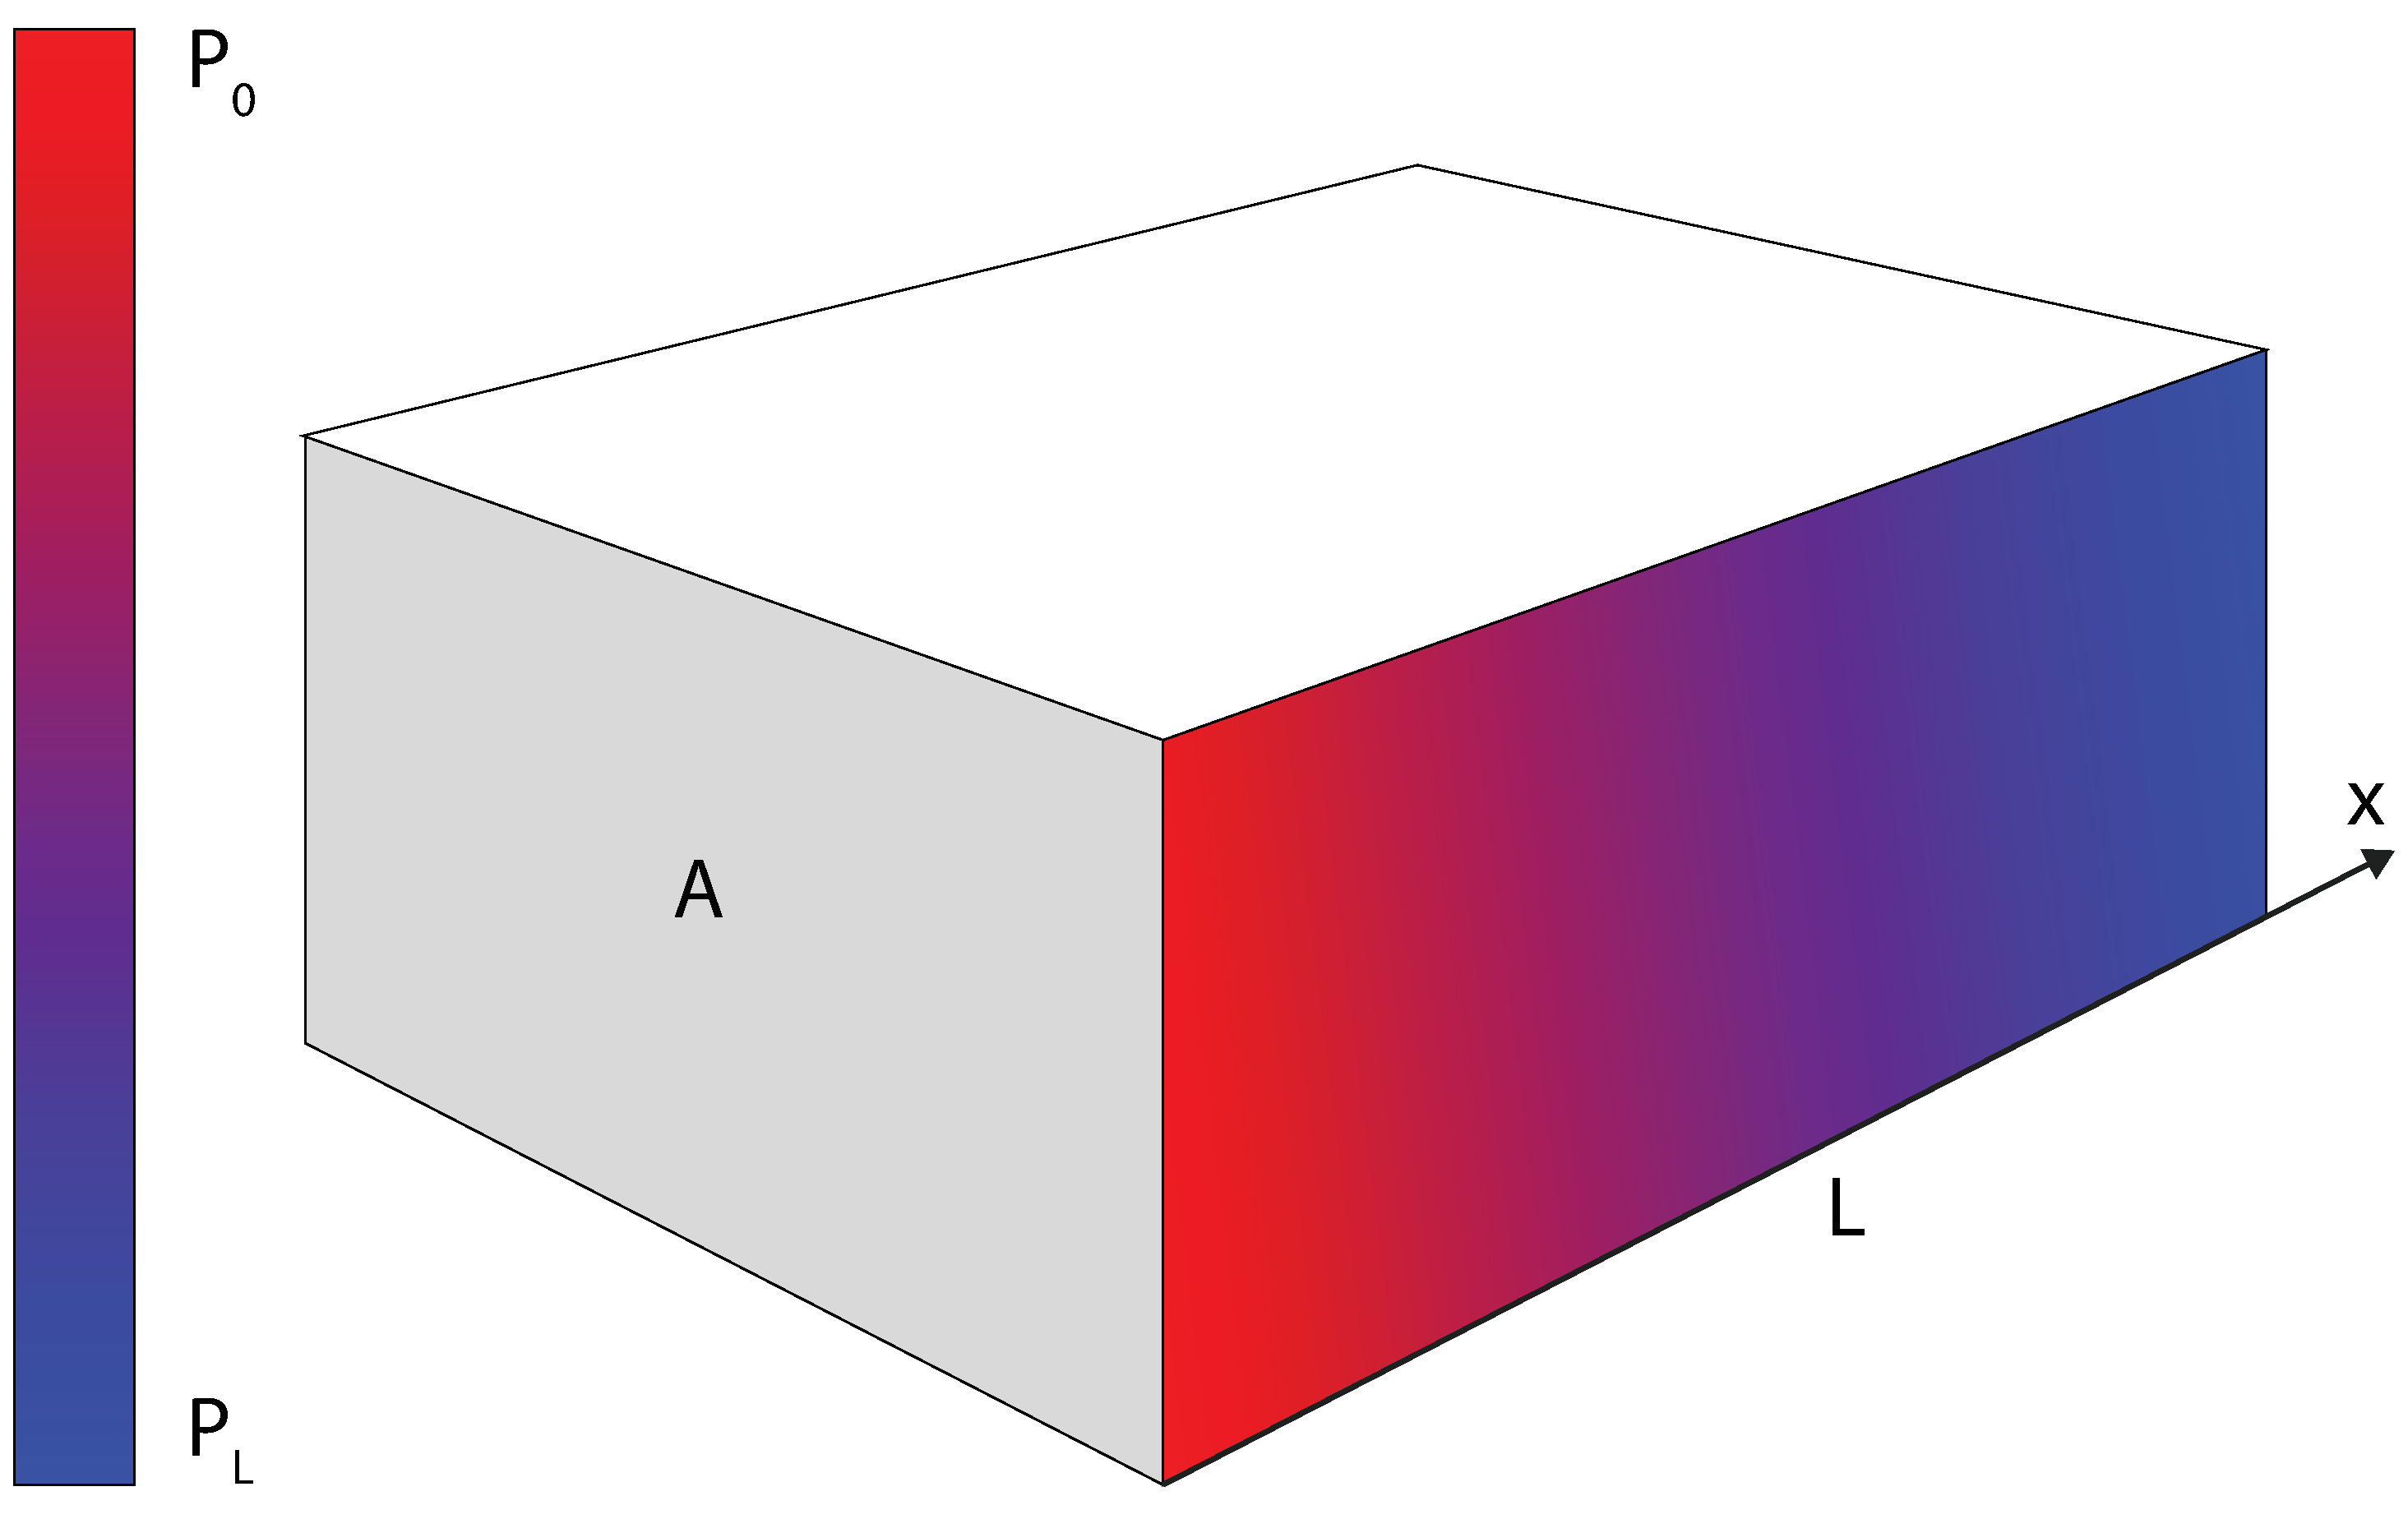
\includegraphics[width=0.75\textwidth, trim=0cm 0cm 0cm 0cm, clip]{kinetic_theory/figures/darcy.eps}
\end{center}
\caption{A box with volume $V=LA$ with fixed pressure values at $x=0$ and $x=L$. The volumetric flow rate $Q$ through a cross sectional area $A$ is given by Darcy's law in equation \eqref{eq:darcy_1}}.
\label{fig:darcys_law}
\end{figure}
The one dimensional version of Darcy's equation is given as 
\begin{align}
\label{eq:darcy_1}
	u = \frac{Q}{A} = \sigma_D\frac{\Delta P}{ L},
\end{align}
where $u$ is the \textit{volumetric flux} (volumetric flow rate per unit area), $\Delta P = P_0 - P_L$ is the pressure difference, $A$ is the cross sectional area; the area of the material orthogonal on the flow direction and $L$ is the length of the material in the flow direction. $\sigma_D$ is the proportionality constant that can be written as
\begin{align}
	\sigma_D = \frac{k}{\mu},
\end{align}
where $\mu$ is the viscosity and $k$ is the permeability.
\section{Permeability}
\label{sec:permeability}
The motivation of introducing the concept permeability is to separate the proportionality constant into two parts; one that depends on the liquid only, the viscosity $\mu$, and the permeability, a material specific constant $k$. This means that we in principle can do an experiment with a liquid with known viscosity, say water, and measure the permeability of some material (Darcy studied a sand filled cylinder in his original experiment). Once you know the permeability, you are able to predict the flow rate through the material for \textit{any} other liquid with a well known viscosity. This is of great importance for i.e. the oil industry where they ideally would like to take a sample of the rock in which the oil and/or gas is confined, measure the permeability with e.g. air, and then use this to predict the recovery rate.\\
This is of course not completely true in all circumstances. While Darcy originally found the relation as an empiric equation based on experiments, it can be derived from the Navier-Stokes equations. Darcy's law is only correct if the fluid flow satisfies the no-slip condition.
\section{Macroflows and microflows}
\label{sec:theory_of_fluids_microflows}
In the 1990s H. Bau and J. Zemel performed experiments on microchannel flow in which they found clear deviations from what was expected from the theory\cite{karniadakis2005microflows}. It is useful to introduce the terms \textit{microflows} for flow in geometries where the distance between the channel walls is of order micrometer or smaller, and \textit{macroflows} for larger systems (milimeter and above). Flow at microscales differ from macroscales because of effects that can be classified into four groups
\begin{itemize}
\item noncontinuum effects,
\item surface-dominated effects,
\item low Reynolds number effects, and
\item multiscale and multiphysics effects.
\end{itemize}
In this thesis, we focus on the noncontinuum effects which are briefly discussed in section \ref{sec:continuum_breakdown}, and the surface-dominated effects as the slip condition described in section \ref{sec:slip_length}. See \cite{karniadakis2005microflows} for details about the effects of low Reynolds number, multiscale and multiphysics. 

\section{The breakdown of continuum}
\label{sec:continuum_breakdown}
As we discussed in section \ref{sec:continuum}, a fundamental assumption in the NSE is that the space is continuous, but we know that in reality, the mass of the fluid is concentrated in the center of the atoms. We often assume that the mass is uniformly distributed in the volume element of which the conservations laws are applied on. This is known as the \textit{continuum hypothesis} and is invalid when the \textit{mean free path} $\lambda$, the average distance a particle moves between collisions, becomes large compared to some characteristic length $L$ in the system, i.e. the diameter of a channel\cite{karniadakis2005microflows}. This property is quantified through the \textit{Knudsen number}
\begin{align}
	\text{Kn} = \frac{\lambda}{L}.
\end{align}
From the kinetic theory we can calculate the mean free path (this is done in section \ref{sec:mean_free_path_calculation})
\begin{align}
	\lambda = \frac{m}{\sqrt 2 \pi d \rho_n} = \frac{k_B T}{\sqrt 2 \pi d^2 P},
\end{align}
where $\rho_n$ is the number density and $m$ and $d$ are the mass and diameter of the particles. By using the ideal gas law $P = \rho_n k_BT$, we can replace the density with the pressure $P$ and the temperature $T$. Here $k_B$ is Boltzmann's constant. For Knudsen numbers smaller than $10^{-2}$, the continuum hypthosis is valid and we can use continuum equations like the NSE and the Euler equations \cite{karniadakis2005microflows}. It turns out that the Knudsen number is very useful, so we will get back to it in section \ref{sec:knudsen_number}.

\section{Slip velocity}
\label{sec:slip_length}
The usual boundary condition we insert when solving the NSE is the no-slip condition where
\begin{align}
	\vec u(\vec r; t) = 0 \qquad \vec r \in \partial\Omega
\end{align}
where $\partial\Omega$ defines the boundary domain. The history of the no-slip condition was studied by Day\cite{day1990no}, based on the work of Stokes in the 19th century. Stokes compared theoretical results to experiments for pendulums of different kinds and concluded that
\begin{aquote}{Stokes, 1901}
	I shall assume, therefore, as the conditions to be satisfied at the boundaries of the fluid, that the velocity of a fluid particle shall be the same, both in magnitude and direction, as that of the solid particle with which it is in contact. The agreement of the results thus obtained with observation will presently appear to be highly satisfactory.
\end{aquote}
In Day's detailed study of the no-slip condition, he says
\begin{aquote}{Day, 1990}
	Looking back, it appears that the acceptance of a more general no-slip condition was prolonged because of experimental shortcomings, not because of a lack of the \'appropriate\' theoretical solutions to fluid flow problems.
\end{aquote}
In other words, the theoretical framework that existed already in the time of Stokes were complete enough to include both slip and no-slip solutions. In fact, Maxwell predicted slip velocity in a paper already in 1867\cite{maxwell1879stresses}, but the experiments the next 50 years seemed to more or less confirm the no-slip condition.\\
That a fluid has a slip velocity is rather obvious when reading Klinkenberg's nice argument
\begin{aquote}{L.J. Klinkenberg, 1941}
Consider a layer adjacent to the wall which is thinner than the mean free path $\lambda$ of the gas molecules, so that practically a molecule does not collide with other molecules present in this layer. At a given moment half of the gas molecules in this layer will have a component of velocity moving towards the wall; the other half in the opposite direction. The molecules moving towards the wall have had their last collision somewhere in the flowing mass, and, therefore, will have an average velocity component in the direction of flow different from zero. A part of this average velocity component will be lost in colliding with the wall. Even if the molecules lose it entirely, then still the average velocity component in the direction of flow of all the molecules contained in the layer will amount to half of the average velocity component of the molecules moving towards the wall. The gas in the layer, therefore, will have a finite rate of flow.
\end{aquote}
It is convenient to introduce the concept of \textit{slip length} $l_s$ to be able to quantify the slip velocity. Slip length is defined as the distance into the wall we would have to extrapolate a velocity profile for it to reach zero value, see figure \ref{fig:slip_length}.
\begin{figure}[h!]
\begin{center}
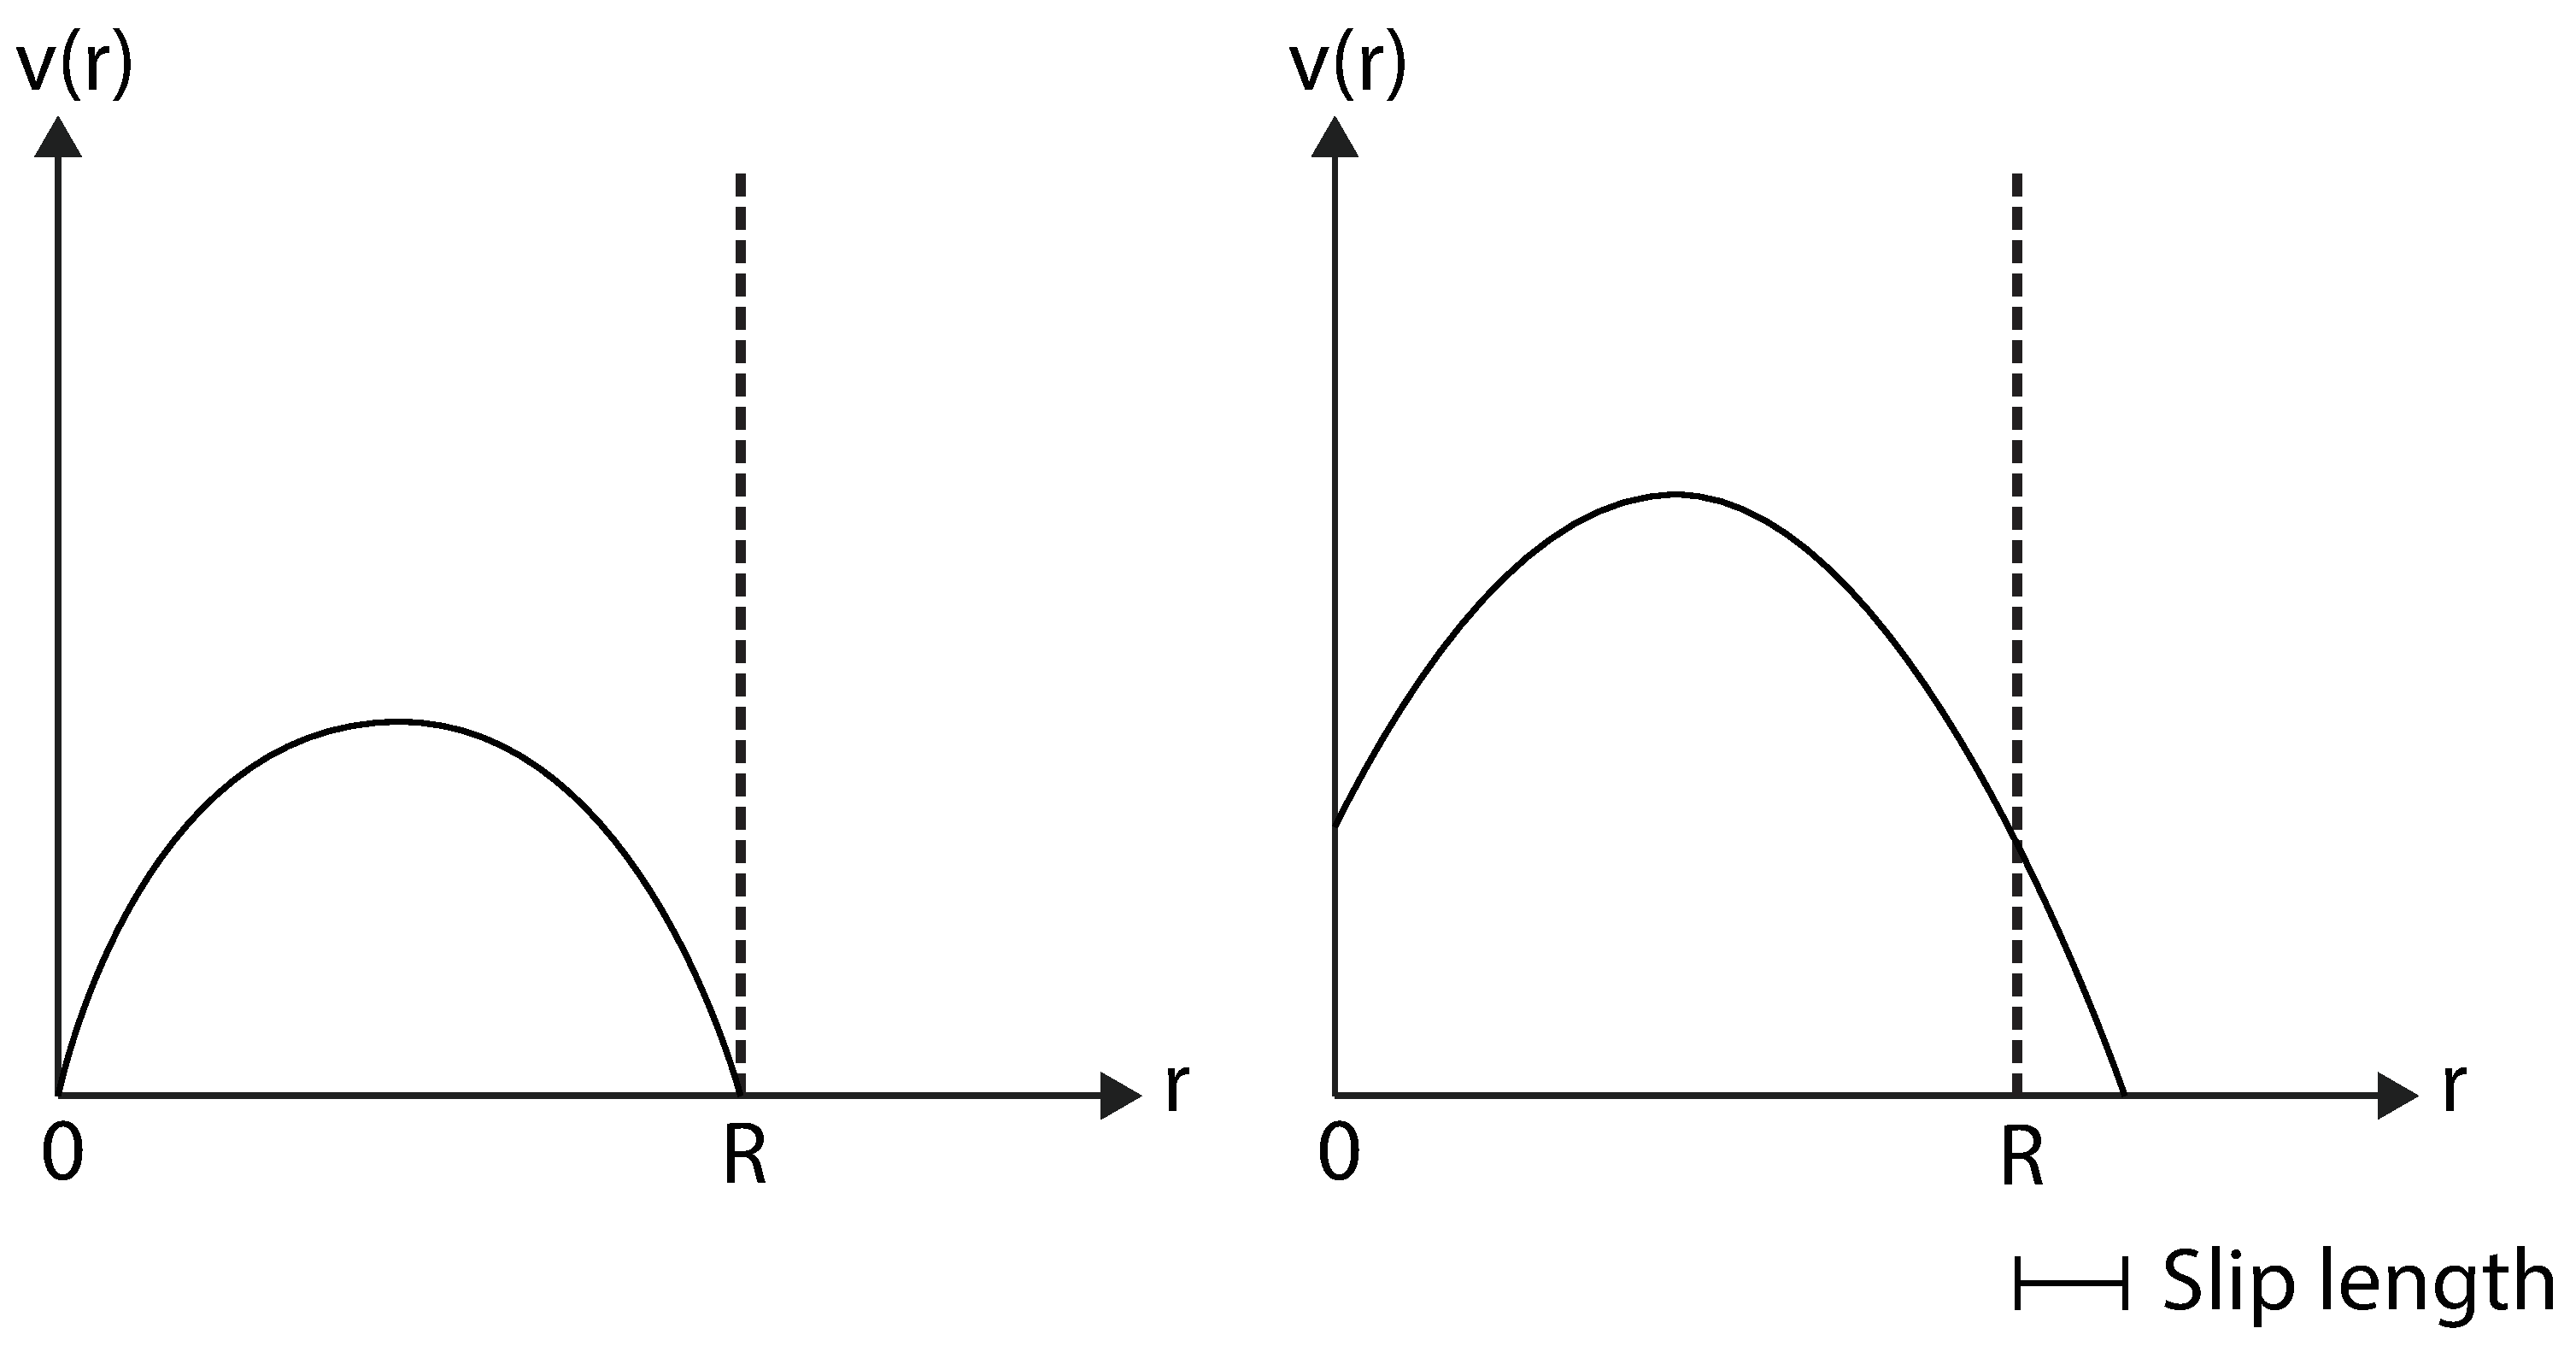
\includegraphics[width=0.8\textwidth, trim=0cm 0cm 0cm 0cm, clip]{DSMC/figures/slip_length.eps}
\end{center}
\caption{Slip length is the distance into the wall we would have to extrapolate a velocity profile for it to reach zero value. We have the no-slip condition on the left, where the slip length is zero whereas we have a non-zero slip length on the right.}
\label{fig:slip_length}
\end{figure}
Maxwell theory predicts the following relation between the slip length and the mean free path
\begin{align}
	\label{eq:noslip_sliplength}
	l_s = \alpha \lambda,
\end{align}
where $\alpha\approx 1.15$ is the slip coefficient \cite{morris1992slip}. The effects of slip velocity become more apparent when the channel diameter is of the same order as the mean free path. By introducing the dimensionless slip length
\begin{align}
	l_s^* = \frac{l_s}{ L} = \alpha \frac{\lambda }{ L} = \alpha \text{Kn},
\end{align}
we see that the ratio of the slip length to the channel diameter is proportional to the Knudsen number. The actual slip velocity (the average velocity of the molecules right next to the wall) can be written as
\begin{align}
	\label{eq:linear_slip_velocity}
	v_{\text{wall}} = \alpha\lambda\frac{\dm v}{\dm n},
\end{align}
where $n$ is the direction normal on the wall\cite{klinkenberg1941permeability}. We call this a \textit{first order} slip model since it is contains only the first derivative of the velocity. Higher order models exists and give corrections that are important in nanoporous media (which is defined in section \ref{sec:nanoporous_media}) where the channels that contribute to flow are of nanometer scale.
\section{Knudsen number}
\label{sec:knudsen_number}


To get an idea of the length scales where the Knudsen number is about unity, the mean free path for helium at $T=$\unit{273}{\kelvin} and $P=1$ atm is\cite{lillestol2001generell} 
\begin{align}
	\label{eq:helium_mfp}
	\lambda_{\text{He}} = \unit{0.17}{\micro\meter} = \unit{170}{\nano\meter}.
\end{align}
This means that for systems where the channels have diameter of a few hundred nanometers, the Knudsen number is around unity, and the continuum hypothesis is invalid. 

\section{Particle models}
\label{sec:theory_of_fluids_atomic_models}
For systems where the continuum hypothesis is invalid, we need other models describing the behaviour of the particles in our system. The first idea that might pop our minds might be to study the system at the atomic level. The equations of motion and hence the dynamics of a system can in principle be calculated directly from quantum mechanics by solving Schr\"{o}dinger's equation. Since this requires calculating the wave function of every atom with complex atomic interactions, the size of the system needs to be very small with today's computers. An alternative, popular approach is to use a parameterized potential $U(\vec r^N)$ ($\vec r^N$ being the positions of all atoms), and calculate the forces through the gradient of $U$. Newton's equations of motion is then integrated and the dynamics of the system are determined in a classical, deterministic way where important effects from quantum mechanics are embedded in the potential. This method is called \textit{Molecular Dynamics} and is studied in chapter \ref{chap:md}. Molecular Dynamics is orders of magnitudes faster than models solving Schr\"{o}dinger's equation, but it still needs a detailed describtion of the dynamics of every atom in the system. For many problems, this information is redundant because what's really important is the statistical properties of the system. In statistical mechanics, we don't need the full information about every single atom. We can then develope models using statistical mechanics and save a lot of computation power compared to Molecular Dynamics. One such model is called Direct Simulation Monte Carlo and is studied in chapter \ref{chap:dsmc}. The fundamental equation in this case is the Boltzmann equation, which we derive in section \ref{sec:boltzmann_equation}. In the limit of low Knudsen numbers, these models do of course converge towards the continuum models. It is convenient to classify different flow regimes depending on the Knudsen number.
\section{Flow regimes}
We can divide the entire Knudsen range into different regimes enabling us to get an overview of which equations and models that are valid for which Knudsen numbers. In the low Knudsen number limit, the continuum hypothesis is valid and we can in principle use any of the models we have discussed. The continuum approach is here of course preferable since it more computationally efficient compared to the particle models. At some point (Kn$\geq 0.01$), the no-slip boundary condition is invalid and we need to incorporate this into the models solving the NSE in order to get accurate solutions. Here starts the slip regime. When the Knudsen number approaches 0.1, we start to see transitional flow where the flow is laminar near the edges and turbulent in the middle of the material, before we at Knudsen numbers larger than 10 have free molecular flow where the particles almost never interact with each other. This is illustrated in figure \ref{fig:flow_regimes} where we have included the regions where different equations are valid.
\begin{figure}[h!]
\begin{center}
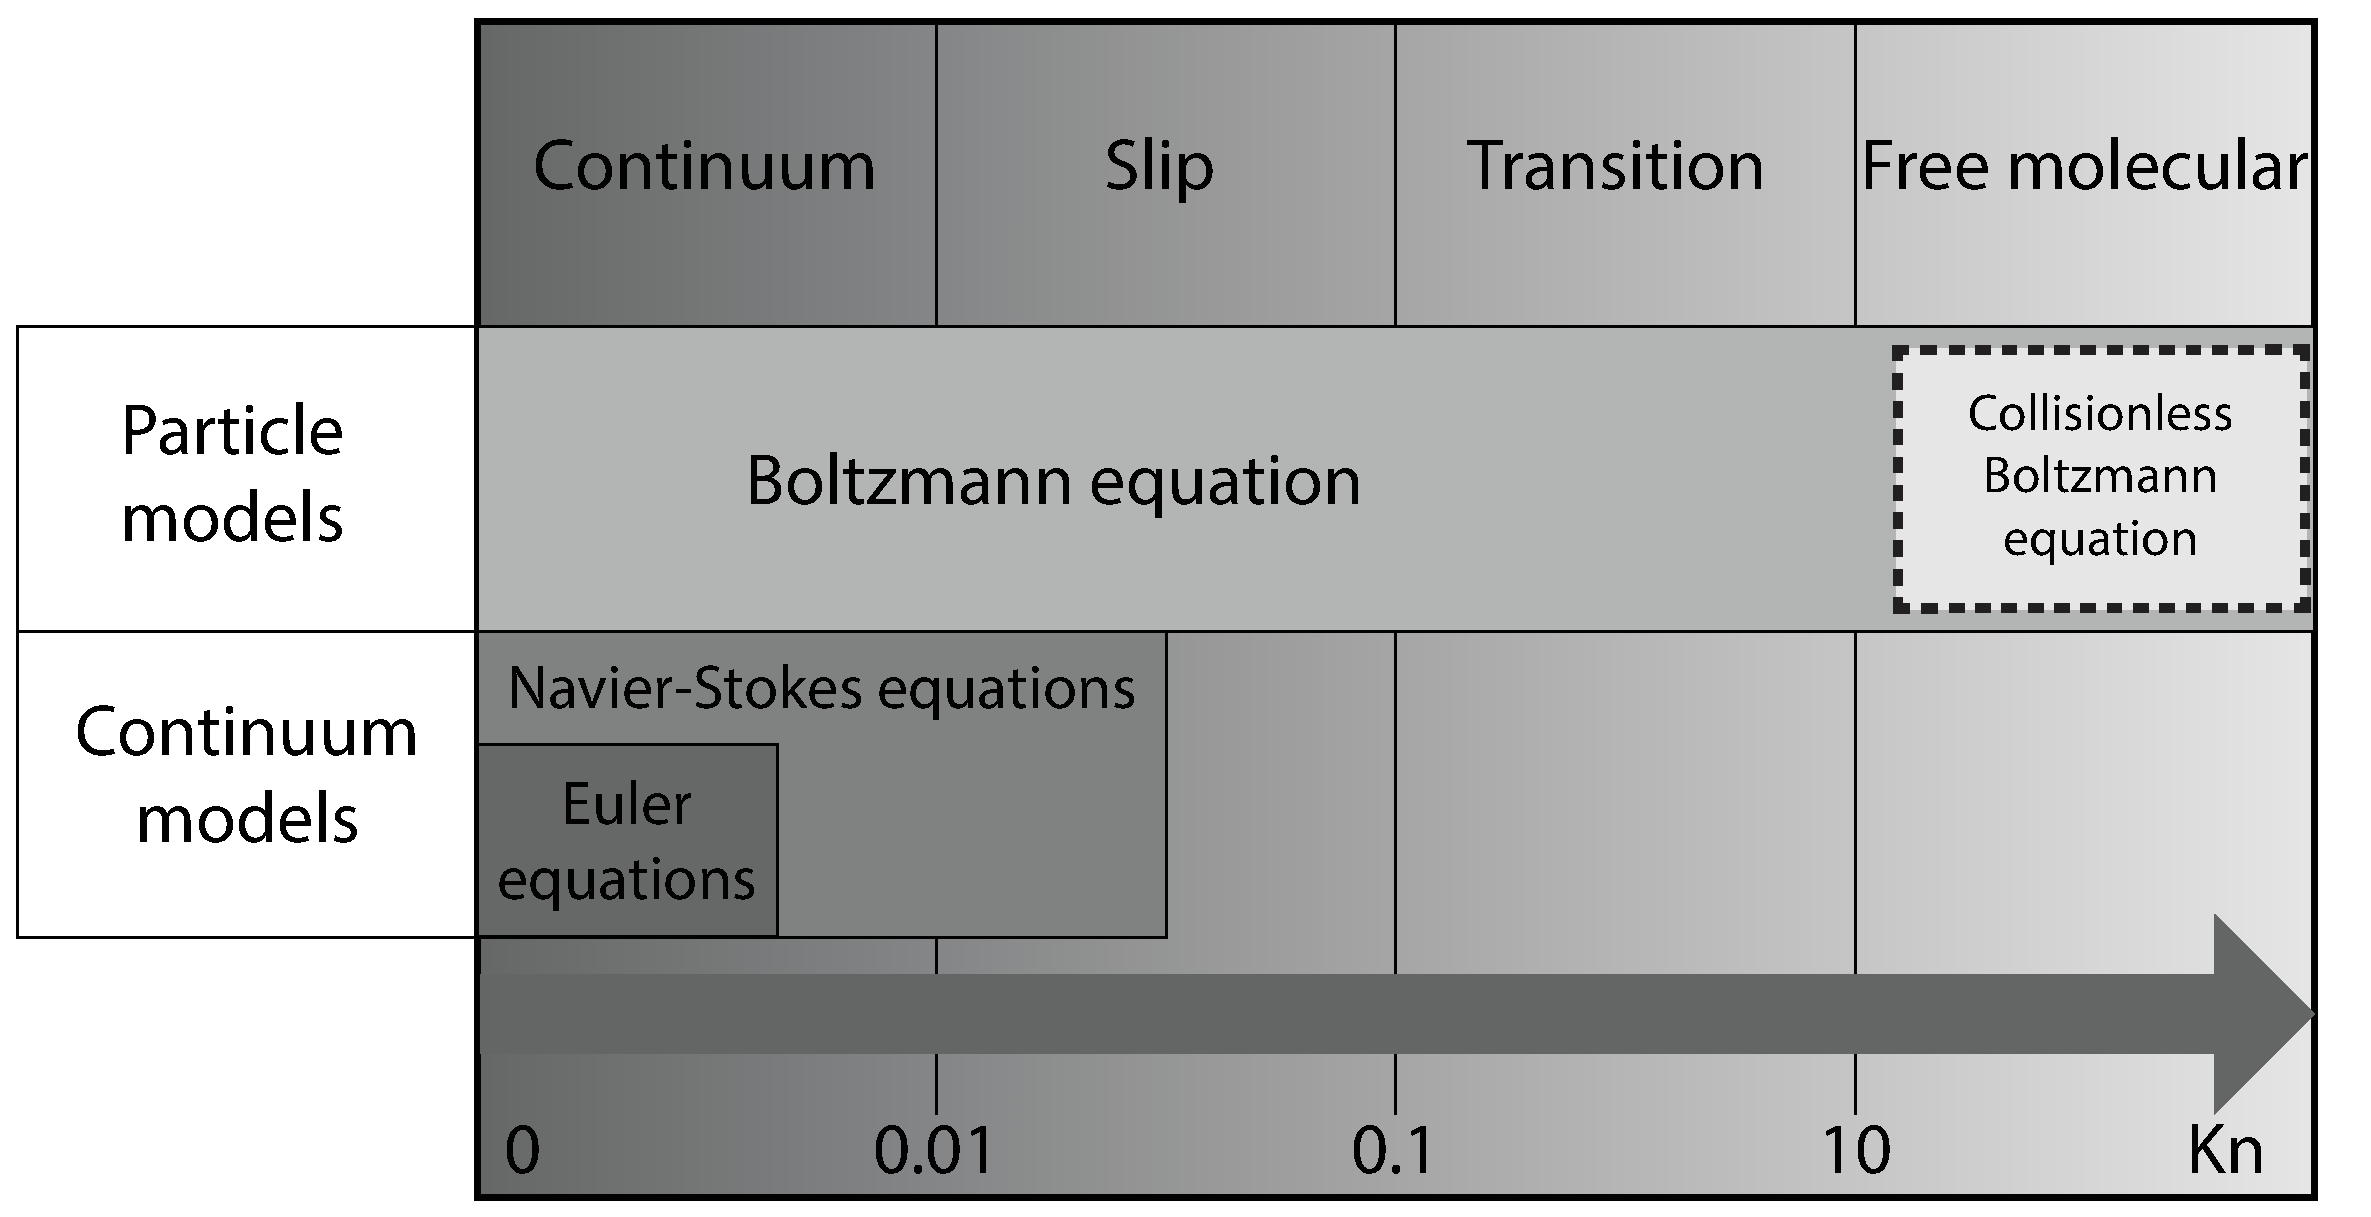
\includegraphics[width=0.8\textwidth, trim=0cm 0cm 0cm 0cm, clip]{figures/flowregimes.eps}
\end{center}
\caption{The four flow regimes covering the important regions in the Knudsen number range where different flow types appear. In the low Knudsen number limit, the fluid can be assumed to be a continuum and we can use equations like the Euler equation or the NSE. For larger Knudsen numbers, the no-slip boundary condition is invalid and we need a model satisfying slip velocity. We reach the transition flow regime at Kn$\approx 0.1$ where the continuum models do no longer hold, even with slip boundary conditions. In the high Knudsen regime particle collisions are so rare that it is classified as free molecular flow. In this range, the collisionless Boltzmann equation is valid (see section \ref{sec:boltzmann_equation}).}
\label{fig:flow_regimes}
\end{figure}
\section{Nanoporous media}
\label{sec:nanoporous_media}
A porous medium is a material with pores and channels (the pore network) available for fluids. See figure \ref{fig:history_porous_media}. 
\missingfigure{Make a sketch of a porous medium.}
  \section{The Klinkenberg effect}
In 1941, L.J. Klinkenberg published a paper explaining the discrepancies that was found in experiments when measuring the permeability for both liquids and gases in the same material\cite{klinkenberg1941permeability}. His discoveries were of great importance in the oil industry
\begin{aquote}{Klinkenberg, 1941}
	It has become common practice in the oil industry to determine the permeability of core material with dry air; the equipment usually employed for this determination is arranged to operate with the outlet of the sample at or near atmospheric pressure.
\end{aquote}
He introduced a linear scaling function $f_c(\text{Kn})$ that relates what he called the \textit{apparent permeability} $k_a$ - the permeability measured in the lab for a fluid with arbitrary density - to the \textit{absolute permeability} $k_\infty$, the permeability for a liquid in the high density limit. The absolute permeability is a constant dependent only on the porous medium. The relation is given as
\begin{align}
	k_a = f_c k_\infty = \left(1 + 4\alpha\frac{\lambda}{L}\right)k_\infty = \left(1 + 4\alpha\text{Kn}\right)k_\infty,
\end{align}
where $L$ is the diameter of the channel and $\alpha\approx 1.15$ is the no-slip factor in equation \eqref{eq:noslip_sliplength}. Since the mean free path is proportional to the inverse pressure, we can write the scaling function as
\begin{align}
	f_c = \left(1 + \frac{b}{\bar P}\right),
\end{align}
where $b$ is a constant depending on the material. In figure \ref{fig:klinkenberg_correction_factor}, we see that the Klinkenberg correction factor predicts a permeability that almost fifty times higher for a gas in a material with $\text{Kn}=10$. The figure also contains the Knudsen correction factor which is discussed in the next section. The Klinkenberg correction factor is derived using the first order slip velocity in equation \eqref{eq:linear_slip_velocity} which is not sufficient for high Knudsen numbers as we will see in section \ref{sec:results_for_simple_geometries}. Based on higher order slip velocity models, one can derive better permeability corrections. 
\begin{figure}[h]
\begin{center}
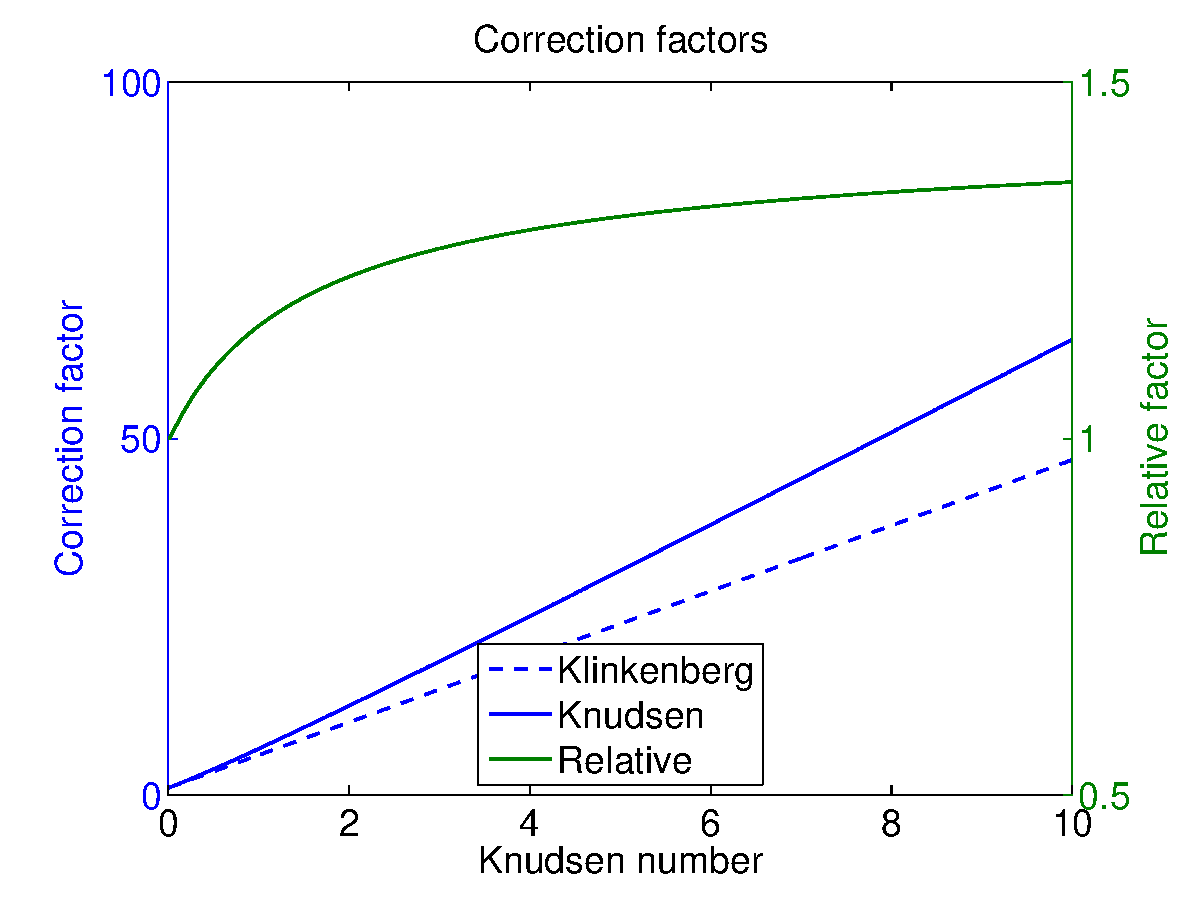
\includegraphics[width=\textwidth, trim=0cm 0cm 0cm 0cm, clip]{figures/klinkenberg.eps}
\end{center}
\caption{A comparison between the Klinkenberg factor and the Knudsen factor shows that slip velocity leads to even higher corrections to the permeability than what the Klinkenberg factor predicts. We see that in the high Knudsen number limit ($\text{Kn}=10$), we can expect an increase of permeability by a factor 50 compared to a liquid or a high density gas. The line labeled \textit{Relative} shows the ratio between the Knudsen correction and the Klinkenberg correction factors.}
\label{fig:klinkenberg_correction_factor}
\end{figure}

\section{Knudsen's correction}
\label{sec:knudsen_correction}
Beskok and Karniadakis (1999) developed another correction factor that uses a second order slip velocity model 
\begin{align}
	\label{eq:knudsen_correction}
	f_c = [1 + \alpha(\text{Kn})\text{Kn}]\left[1 + \frac{4\text{Kn}}{ 1 + \text{Kn}}\right],
\end{align}
where $\alpha(\text{Kn})$ is given as\cite{civan2010effective}
\begin{align}
	\alpha(\text{Kn}) = \frac{\alpha_0}{1 + \frac{A}{\text{Kn}^B}}
\end{align} 
where $A=0.170$, $B=0.4348$, and $\alpha_0=1.358$. These are fitted parameters based on a large dataset of Loyalka and Hamoodi (1990). We see in figure \ref{fig:klinkenberg_correction_factor} that the Knudsen factor predicts approximately 40\% higher correction than the Klinkenberg factor. In chapter \ref{chap:dsmc_results} we will check the validity of this correction factor for a simple cylinder, and discuss the practical problems we meet when studying flow in complex geometries where the system does not simply have one Knudsen number, but rather a distribution of Knudsen numbers.
\end{chapter}

\begin{part}{Direct Simulation Monte Carlo}
\label{part:dsmc}
\begin{chapter}{Kinetic theory}
  \label{chap:kinetic_theory}
  The kinetic theory of gases is a microscopic theory that describes the behavior of gases on the molecular level. A system of $N$ particles is fully described by the $3N$ momentum components combined with the $3N$ spatial coordinates. Together, this forms a $6N$ dimensional phase space where each point represents the state of the system in an ensemble. We start this chapter by introducing the distribution function, the concepts of microstates, macrostates and ensembles in section \ref{sec:kinetic_theory_distribution_function}, before we in section \ref{sec:kinetic_theory_ensemble_averages} explain how we measure the macroscopic observables which are average values over all the states in an ensemble. Then we have a brief discussion about ergodicity in section \ref{sec:kinetic_theory_ergodicity} which is a very important assumption when we start measuring physical quantities in a numerical statistical mechanics model such as Direct Simulation Monte Carlo (chapter \ref{chap:dsmc}) and Molecular Dynamics (chapter \ref{chap:md}). In section \ref{sec:boltzmann_equation} we derive the Boltzmann equation which is the fundamental equation that governs the behavior of the distribution function. We then define what an equilibrium state is which we use to derive the Maxwell-Boltzmann velocity distribution in section \ref{sec:maxwell_boltzmann_distribution}. As we might remember, the Knudsen number is an important dimensionless quantity that we use to quantify how important surface and non-continuum effects are. The Knudsen number is the ratio between the mean free path $\lambda$ and some characteristic length $L$ of the system. In section \ref{sec:mean_free_path_calculation} we calculate the mean free path which is used to compute the mean collision time $\tau_\text{coll}$, which is important to choose a good timestep in the Direct Simulation Monte Carlo model in chapter \ref{chap:dsmc}.
\section{The distribution function}
\label{sec:kinetic_theory_distribution_function}
A point $(\vec r, \vec v)$ in the phase space describes what is called a \textit{microstate} and contains a massive amount of information. Given this point, we would know the position and velocity to \textit{every} particle in the entire system. In a liter of an ideal gas under standard pressure, the number of particles is of order $10^{22}$ \cite{garcia2000numerical}, so if each of these $6N$ coordinates were represented as an 8 byte \textit{double} on a computer, we would need more than $10^{11}$ terabytes of memory just to store all the information. This approach would be very inconvenient and, fortunately, not at all necessary. The really interesting properties in a system are the macroscopic ones, like energy, temperature, pressure, volume, average velocity among others. For example, the total energy in a gas consisting of $N$ particles is calculated as
\begin{align*}
	E = \sum_{i=1}^N \frac{1}{2} m_i v_i^2 + V(\vec r),
\end{align*}
where $m_i$ is the mass of particle $i$, $v_i$ is its scalar velocity and $V(\vec r)$ is the total potential energy in the system depending on the full $3N$-dimensional spatial coordinate $\vec r$.\\
Given a microstate, what happens if we switch two particles, say particle $i$ and $j$? If particle $i$ had velocity $\vec v_i = \vec u$ and particle $j$ had some other velocity $\vec v_j = \vec w$, we could quickly swap them so that $\vec v_i = \vec w$ and $\vec v_j = \vec u$ (theoretically of course, it would be a difficult task in an experiment). If their masses are identical, the total energy of the system would not change, but since \textit{we} know that we switched the two particles, we could want to count this as another microstate. We could in principle paint the particles with different colors, or maybe just label them with their own unique number. However, in a real, mono-atomic gas, we can't really tell the difference if particle $i$ and $j$ secretly agreed to switch places without telling us. If they did so, it would not count as different microstates, the system remains exactly the same. We say that the particles are \textit{indistinguishable}.\\
If we instead increase the velocity of particle $i$, we can reduce some another particle $j$'s velocity to keep the total energy constant. Even though the macroscopic property \textit{energy} is unchanged, there is a (theoretically) measurable difference between these two states. The set of all microstates that share the same macroscopic state variables (a \textit{macrostate}) forms an ensemble of systems. A much used ensemble is the microcanonical ensemble (NVE) with a constant number of particles $N$, constant volume $V$ and constant energy $E$. Increasing the velocity of particle $i$ while at the same time reducing particle $j$'s velocity just enough to remain the energy unchanged does not change the particle number $N$, the volume $V$ or the energy. So these two different microstates would both be in the same ensemble.\\

In a typical system, the number of microstates in a macrostate is so huge that the phase space points can be described by a continuous density function $f(\vec p, \vec r, t)$ without losing any important information \cite{mcquarrie1973statistical}. The input parameters are the $3N$ momentum components, the $3N$ spatial coordinates plus time. This function is often called a \textit{distribution function}, normalized so that
\begin{align}
	\iint\! f(\vec p, \vec r, t) \dm \vec p\dm \vec r = N,
\end{align}
where $\dm \vec p\dm \vec r=\dm p_1\dm p_2...\dm r_{3N}$ is the $6N$ dimensional phase space volume element. This density function does not contain the information about the \textit{exact} positions or momenta of the particles, but the \textit{probability} to find the system in a state around a given phase space point. We can then use it to calculate measurable, macroscopic average values. 

\section{Ensemble averages}
\label{sec:kinetic_theory_ensemble_averages}
Given the distribution function $f$, we can calculate any ensemble average (which will be the measurable, macroscopic properties of the system) by interpreting $f$ as a probability distribution (it needs the factor $1/N$ to be normalized to one) that gives the probability of finding a particle at position $\vec r + \dm \vec r$ with momentum in the range $\vec p + \dm\vec p$ at the time $t$. We can then use the standard expectation value expression to calculate a macroscopic property $\bar A$
\begin{align}
	\label{eq:ensemble_average}
	\bar A(t) = \frac{1}{ N}\iint\! A(\vec p, \vec r, t)f(\vec p, \vec r, t)\dm \vec p\dm\vec r.
\end{align}
This could for example be the total energy
\begin{align}
	\bar E(t) &= \frac{1}{ N}\iint\! E(\vec p, \vec r, t)f(\vec p, \vec r, t)\dm \vec p\dm\vec r \\
	&= \frac{1}{ N}\iint\! \left(V(\vec r) + \sum_{i=1}^N \frac{\vec p_i^2}{2m_i} \right)f(\vec p, \vec r, t)\dm \vec p \dm \vec r,
\end{align}
where $\vec p_i$ is the momentum of particle $i$. Any other quantity of interest can in principle be measured in the same way. 

\section{Ergodicity}
\label{sec:kinetic_theory_ergodicity}
The ensemble average calculates the average value of some macroscopic quantity given the distribution function $f$. Usually, we don't have the distribution function, except in some very simple theoretical calculations. Even then, it might be difficult to compute the integral in equation \eqref{eq:ensemble_average}. The usual situation when we do numerical statistical mechanics is that we have a way to explore the phase space, hoping that it helps us visit states with probabilities according to the given ensemble. Many Monte Carlo techniques (such as the Metropolis algorithm) allow us to go to a new, random point in the phase space, and calculate the probability of going from the current state to the new state. From this, we can count the number of times we have visited different regions of the phase space and create a histogram or maybe, if we're lucky, fit some existing probability distribution to our data.\\
Another approach is to let the rules of physics take us around in the phase space, from one state to another, following Newton's equations of motion. Imagine that at $t=0$, our system is in some microscopic state (a single phase space point ($\vec r(0), \vec p(0)$)) and at a later time $t=\tau$ has moved to ($\vec r(\tau), \vec p(\tau)$). Between these two points, the system has moved through many other points, exploring the phase space. It seems reasonable that in the limit of infinite time, the time evolution should visit the phase space points according to the density given by $f$. If not, it wouldn't make any sense even talking about $f$, since it is the time evolution we, as humans, are experiencing in the real physical world.\\
This is called the ergodicity hypothesis, the assumption that a system following the laws of physics, explores the phase space with the probability of being in a region proportional to the density in that region. The average value of a macroscopic quantity $A$ is then found as
\begin{align}
	\bar A = \lim_{t\rightarrow \infty} \frac{1}{t}\int_0^{t} A(\vec r(t'), \vec p(t'), t')\dm t'.
\end{align}
  \section{The Boltzmann equation}
\label{sec:boltzmann_equation}
In the section \ref{sec:kinetic_theory_distribution_function}, we introduced the distribution function $f$ that describes the density in a $6N$ dimensional phase space. Now, if we know the distribution function at $t=0$, we could in principle compute any property of the system. But at a later time $t=\tau$, the distribution function might have changed, unless, of course, $\partial_t f = 0$ (in which the system would be in what we call an equilibrium state). We can, by applying conservation of probability, derive an equation of motion for $f$. This equation is called the Boltzmann equation. It describes how $f$ evolves through time by assuming that any change of density (read probability) around a point $(\vec r, \vec v)$ at the time $t$ must be due to
\begin{itemize}
	\item flow through a surface in the phase space,
	\item an external force, or
	\item internal collisions.
\end{itemize}
All three will change $f$ in different ways. For simplicity, we will first assume that the particles do not collide and derive the \textit{collisionless Boltzmann equation}. But do not worry, we will add the collision term later and end up with the full Boltzmann equation.

\subsection{The collisionless Boltzmann equation}
Consider the density around the phase space point $(\vec r,\vec v)$ at the time $t$. If we assume no forces, and that the total number of particles has not changed, a time $dt$ later, the density has moved to $(\vec r + \vec vdt, \vec v)$. Conservation of probability states that any change of $f$ within a volume $\Omega$ must flow through the boundary $\partial \Omega$
\begin{align}
	\frac{\dm }{\dm t}\int_\Omega f \dm \vec r \dm \vec v &= -\int_{\Omega_v}\dm \vec v\int_{\partial \Omega_r} f(\vec v\cdot \vec n_r) \dm S_r\\
	&= -\int_{\Omega_v}\dm \vec v\int_{\Omega_r} \nabla_\vec r\cdot(f\vec v) \dm \vec r = -\int_{\Omega} \nabla_\vec r\cdot(f\vec v) \dm \vec v\dm \vec r
\end{align}
which becomes
\begin{align}
	\dpart{f}{t} + \nabla_\vec r \cdot(f\vec v) = \dpart{f}{t} + \vec v\cdot\nabla_\vec r f = 0
\end{align}
since $\vec v$ is independent of $\vec r$. We can extend this equation by adding the effects of an external force $\vec F$ that changes the velocity in the same way as the position was changed above (except for the factor $1/m$)
\begin{align}
	\label{eq:collisionless_boltzmann}
	\dpart{f}{t} + \vec v\cdot\nabla_\vec r f + \nabla_\vec v \cdot \frac{\vec F}{ m}f = 0,
\end{align}
which we call the collisionless Boltzmann equation. It is a good approximation to describe the dynamics of very dilute gases where intermolecular collisions occur rarely. But we should not ignore collisions between particles, so as promised, we will now see that by treating collisions will appear as an additional term.
\subsection{The collision operator}
We consider a dilute gas so we can assume that only binary collisions occur (we ignore the contribution from collisions between three or more particles at a time). We also assume that the total energy and momentum is conserved in all collisions. Then consider two particles $i$ and $j$ moving towards each other with velocities $\vec v$ and $\vec v_1$, and relative velocity $\vec g = \vec v - \vec v_1$. We define particle $i$ as the \textit{incident} particle and $j$ as the \textit{target} particle. After the collision, the particles will have velocities $\vec v'$ and $\vec v_1'$ with relative velocity $\vec g' = \vec v' - \vec v_1'$. In order to make the calculations simpler, we change the frame of reference. If we choose the target particle as initial frame of reference, we see that the velocity of the incident particle becomes $\tilde {\vec v} = \vec g$ and $\tilde {\vec v}' = \vec g'$. Since momentum is conserved, we know that the relative velocity must remain constant $|\vec g| = |\vec g'|$ during the collision. The direction of $\vec g'$ is given by the angles $\phi$ and $\theta$ with $\hat {\vec z}$ along $\vec g$ and $\phi \in [0, 2\pi], \theta \in [0, \pi]$. We can express $\vec g'$ as
\begin{align}
	\vec g' = \vec g - 2\unitvector e(\unitvector e\cdot\vec g),
\end{align}
where $\unitvector e$ is an arbitrary unit vector. \todo{Illustrate this with a figure?} If we multiply by $\unitvector e$, we see that 
\begin{align}
	\unitvector e\cdot \vec g' = \unitvector e\cdot\left[\vec g - 2\unitvector{e}(\unitvector e\cdot\vec g)\right] = -\unitvector e \cdot \vec g
\end{align}
which gives the symmetric relation
\begin{align}
	\vec g = \vec g' - 2\unitvector e(\unitvector e\cdot\vec g').
\end{align}
The angle between $\vec g$ and $\vec g'$ is $\theta$, so
\begin{align}
	\vec g'\cdot \vec g = g^2\cos\theta = g^2(1 - 2\cos \chi),
\end{align}
where $\chi$ is the angle between $\unitvector e$ and $\vec g$ which gives the relation
\begin{align}
	\theta = \pi - 2\chi.
\end{align}
We now define the solid angle element $\dm\Omega=\sin\theta \dm\theta \dm\phi$ about $\vec g'$ 
\begin{align}
	g \dm\Omega &= g\sin\theta \dm\theta \dm\phi = 2g\sin(\pi - 2\chi)\dm\chi \dm\phi\\
	&= 4g\cos\chi\sin\chi \dm\chi \dm\phi = 4\left|\unitvector e\cdot\vec g\right|\sin\chi \dm\chi \dm\phi\\
	&= 4\left|\unitvector e\cdot\vec g\right|\dm^2e,
\end{align}
where $\dm^2e = \sin\chi \dm\chi \dm\phi$ is a solid angle element about $\unitvector e$. In the following, we will calculate the scattering cross section which is the \textit{area} that describes the likelyhood of an incident particle being scattered by the target particle. We denote the number density $\rho_n$ and find that the incident flux is $\rho_n g$. The rate $h_{\dm\Omega}'$ of scattered particles into $\dm\Omega$ is
\begin{align}
	\label{eq:partial_scattering_rate}
	h_{\dm\Omega}' = \rho_n g\sigma \dm\Omega,
\end{align}
where the proportionality constant $\sigma$ is the cross section. We might have several target particles colliding independently of each other which will contribute to the scattering rate. If we have $n_t$ such particles, we obtain the total scattering rate $h_{\dm\Omega}$ by multiplying \eqref{eq:partial_scattering_rate} by $n_t$
\begin{align}
	h_{\dm\Omega} = n_t\rho_n g\sigma \dm\Omega.
\end{align}
The \textit{differential} cross section $\sigma$ depends on $\vec g$ and $\vec g'$, so we denote it as $\sigma = \sigma(\vec g\rightarrow \vec g')$, whereas the \textit{total} cross section $\sigma_T$ is given by integrating over all solid angles
\begin{align}
	\sigma_T = \int \sigma \dm\Omega.
\end{align}
We will now look at particles with velocities in the range $[\vec v, \vec v + \dm\vec v]$ incident on target particles with velocities in the range $[\vec v_1, \vec v_1 + \dm\vec v_1]$. The incident flux is $gf(\vec v,\vec r)\dm\vec v$ and the number of target particles is $f(v_1,\vec r)\dm\vec v_1\dm\vec r$. The rate at which particles with velocity $\vec v_1$ are scattered by particles with velocity $\vec v$ is \todo{Check if these $f$'s should be normalized}
\begin{align}
	f(\vec v)f(\vec v_1) g \sigma \dm\Omega \dm\vec v \dm\vec v_1 \dm\vec r = f(\vec v)f(\vec v_1)4\left|\unitvector e\cdot \vec g\right| \sigma \dm^2e \dm \vec v \dm\vec v_1 \dm \vec r.
\end{align}
The rate of loss is the rate of which particles in $\dm\vec v\dm\vec r$ are being hit by other particles. We can calulate this by integrating over all solid angles $\dm^2 e$ and incident velocities $\dm \vec v$
\begin{align}
	\text{rate of loss} = \left[\int f(\vec v)f(\vec v_1)4\left|\unitvector e \cdot \vec g \right|\sigma \dm^2 e\dm \vec v_1\right]\dm \vec v\dm \vec x.
\end{align}
We also have the inverse event, incident particles with velocity $\vec v'$ hitting target particles with velocity $\vec v_1'$ so that the final velocity of the target particles is $\vec v$. This is calculated with the same idea
\begin{align}
	\text{rate of gain} = \left[\int f(\vec v')f(\vec v_1')4\left|\unitvector e \cdot \vec g \right|\sigma \dm^2 e\dm \vec v_1\right]\dm\vec v\dm\vec x,
\end{align}
since $|\unitvector e\cdot \vec g| = |\unitvector e\cdot \vec g'|$ and $\dm\vec v'\dm\vec v_1' = \dm\vec v\dm\vec v_1$. The total change in the distribution function is given by the functional $J[f]$
\begin{align}
	J[f] &= \int \dm\vec v_1 \dm^2 e4|\unitvector e\cdot\vec g|\sigma[f'f_1' - ff_1]\\
	&= \int \dm\vec v_1 \dm\Omega g \sigma[f'f_1' - ff_1],
\end{align}
where $f = f(\vec r, \vec v, t)$ and $f_1 = f(\vec r, \vec v_1, t)$. The full Boltzmann equation is then given by
\begin{align}
	\label{eq:boltzmann_equation}
	\dpart{f}{t} + \vec v\cdot \nabla_\vec r f + \frac{\vec F}{m}\cdot\nabla_\vec v f = J[f].
\end{align}
In the derivation of the collision operator $J[f]$, we assumed binary collisions only. This is a decent approximation that holds for low densities. By defining the force range $D$ and the dimensionless parameter $\nu = \rho_n D^3$, the Boltzmann equation is valid when $\nu$ is small \cite{mclennan1989introduction}. $D^3$ defines a volume around a particle in which the forces cannot be neglected. This makes $\nu$ the average number of particles within that volume. If that number is small (less than unity) then we can safely neglect collisions between three or more particles.
\section{\textit{H}-theorem}

Boltzmann's $H$-theorem is a powerful result that gives us all the theoretical tools we need to implement the DSMC method. We define the $H$-function as
\begin{align}
	H(t) = \langle \ln f \rangle = \int f(\vec r, \vec v, t)\ln f(\vec r, \vec v, t)d\vec r d\vec v
\end{align}
and differenciate with respect to time
\begin{align}
	\frac{dH}{dt} = \int \dpart{f}{t}\ln f d\vec r d\vec v + \int \dpart{f}{t} d\vec r d\vec v = \int \dpart{f}{t}\ln f d\vec r d\vec v
\end{align}
where we have used that the number of particles is conserved
\begin{align}
	\int \dpart{f}{t}d\vec r d\vec v = \frac{d}{dt} \int fd\vec r d\vec v = \frac{dN}{dt} = 0.
\end{align}
We multiply the Boltzmann equation by $\ln f$ and integrate
\begin{align}
	% \int \dpart{f}{t}\ln f d\vec r d\vec v = -\int (\ln f)\vec v\cdot \nabla_\vec r f d\vec r d\vec v - \int (\ln f) {\vec F\over m}\cdot \nable_\vec v f d\vec rd\vec v + \int \ln f J[f] d\vec r d\vec v
	balle
\end{align}

\section{Maxwell-Boltzmann distribution as equilibrium}
\label{sec:maxwell_boltzmann_distribution}
\begin{align}
	\label{eq:maxwell_boltzmann_distribution}
	P(v_i)\dm {v_i} = \sqrt\frac{m}{ 2\pi k_BT}e^\frac{-mv_i^2}{ 2k_BT}\dm {v_i},
\end{align}
\section{Mean free path}
\label{sec:mean_free_path_calculation}
The collision frequency can be calculated through the mean free path, which is the average distance a molecule travels between collisions. The mean free path for a gas is estimated by looking at the \textit{effective collision area}, see figure \ref{fig:effective_collision_area}. The effective collision area is then
\begin{align}
	A = \pi d^2,
\end{align}
where $d$ is the molecular diameter. Two molecules with velocities $\vec v_1$ and $\vec v_2$ have the relative velocity $\vec v_{rel} = \vec v_1 - \vec v_2$. The norm is given by
\begin{align}
	v_{rel} &= \sqrt{\vec v_{rel}\cdot \vec v_{rel} } = \sqrt{ (\vec v_1 - \vec v_2)(\vec v_1 - \vec v_2)}\\
	&= \sqrt{\vec v_1\cdot \vec v_1 - 2\vec v_1\vec v_2 + \vec v_2\vec v_2}.
\end{align}
The average relative velocity is calculated by assuming that the velocities are completely random and hence not correlated, and that the molecules have the same mean speed $\langle v\rangle$
\begin{align}
	\bar v_{rel} &= \sqrt{\vec v_1^2 + \vec v_2^2} = \sqrt 2 \langle v\rangle,
\end{align}li
During a time $\tau$ and average relative molecular velocity $\sqrt 2 \langle v\rangle$, the total volume sweeped out by the particle is given as
\begin{align}
	V = \sqrt 2 \pi d^2\langle v\rangle \tau,
\end{align}
which in turn gives the number of collisions during such a volume
\begin{align}
	\label{eq:num_collisions}
	n_{coll} = V\rho_n = \sqrt 2 \pi d^2\langle v\rangle \rho_n \tau,
\end{align}
where $\rho_n$ is the number density. The mean free path is then calculated as the length of the path divided by the number of collisions
\begin{align}
	\label{eq:mean_free_path}
	\lambda = \frac{\langle v\rangle \tau}{ \sqrt 2 \pi d^2\langle v\rangle \rho_n\tau} = \frac{1 }{ \sqrt 2 \pi d^2 \rho_n}
\end{align}
\section{Mean collision time}
\begin{align}
	\label{eq:coll_frequency}
	f_{coll} = \rho_n \pi \sigma^2 \langle v_r \rangle
\end{align}
  \section{The Maxwell-Boltzmann distribution}
\label{sec:maxwell_boltzmann_distribution}
We will now find out which $f$ that satisfies equation \eqref{eq:equilibrium_f_relation} which we rewrite by taking the logarithm on both sides
\begin{align}
	\ln f' + \ln f_1' = \ln f + \ln f_1.
\end{align}
This states that the \textit{sum} of of the logarithm of $f$ is unchanged during a collision. As we required in subsection \ref{sec:boltzmann_collision_operator}, energy, momentum and mass are conserved quantities, so $\ln f$ must be a linear combination of these
\begin{align}
	\ln f &= \alpha m + \vec \beta\cdot(m\vec v) - \gamma\frac{mv^2}{2}\\
	&= \alpha m + \frac{m}{2}\frac{\beta\cdot\beta}{\gamma} - \frac{m\gamma}{2}\left(\vec v - \frac{\beta}{\gamma}\right)^2.
\end{align}
We combine all quantities not dependent of $\vec v$ into one parameter $\ln c$ so that
\begin{align}
	\ln f = \ln c - \frac{m\gamma}{2}\left(\vec v - \frac{\vec \beta}{\gamma}\right)^2,
\end{align}
which we can write as
\begin{align}
	\label{eq:almost_maxwell}
	f(\vec r, \vec v) = c\exp\left[-\frac{m\gamma}{2}\left(\vec v - \frac{\beta}{\gamma}\right)^2\right].
\end{align}
By using that 
\begin{align}
	\rho_n(\vec r, t) = \int\!f \,\dm\vec v,
\end{align}
and 
\begin{align}
	\vec v_0 = \langle \vec v\rangle = \frac{1}{\rho}\int\!\vec v f\,\dm \vec v
\end{align}
in addition to the equipartition theorem
\begin{align}
	\frac{3}{2}k_B T = \frac{m}{2}\langle(\vec v - \vec v_0)^2\rangle
\end{align}
we can write equation \eqref{eq:almost_maxwell} as \cite{mclennan1989introduction}
\begin{align}
	\label{eq:maxwell_boltzmann_distribution}
	f(\vec r, \vec v) = \rho_n \left(\frac{m}{2\pi k_B T}\right)^{3/2}e^\frac{-m|\vec v|^2}{2k_BT},
\end{align}
which is the \textit{Maxwell-Boltzmann distribution}. We can integrate out the position part of the distribution to get
\begin{align}
	\label{eq:maxwell_boltzmann_vector_probability}
	P(\vec v)\dm \vec v = \left(\frac{m}{2\pi k_B T}\right)^{3/2}e^\frac{-m|\vec v|^2}{2k_BT} \dm \vec v.
\end{align}
We will use this to validate the DSMC code section \ref{sec:dsmc_code_validation}. Now, let us use this to find some interesting properties of the gas. Given a temperature $T$ and the mass of the particles $m$, what is the average speed of the particles? First, we need to transform the distribution from a vector distribution to a scalar distribution (the magnitude of the velocity might be a more interesting quantity than a given direction). The distribution in equation \eqref{eq:maxwell_boltzmann_vector_probability} is spherical symmetric, so we should transform to spherical coordinates which gives
\begin{align}
	\label{eq:maxwell_boltzmann_scalar_probability}
	P(v)\dm v = 4\pi\left(\frac{m}{2\pi k_B T}\right)^{3/2}v^2e^\frac{-mv^2}{2k_BT} \dm v.
\end{align}
The average speed of the particles can then be found as
\begin{align}
	\label{eq:maxwell_boltzmann_average_speed}
	\langle v\rangle = \int\limits_0^\infty vP(v) \dm v = \frac{2\sqrt 2}{\sqrt \pi}\sqrt\frac{k_B T}{m}.
\end{align}
The particles in a high temperature gas moves faster than particles in a gas with low temperature, as expected. The next important quantity we should compute is the mean free path. We will need that to calculate the Knudsen number from section \ref{sec:knudsen_number}.
  \section{Mean free path}
\label{sec:mean_free_path_calculation}
The mean free path $\lambda$ is the average distance a particle travels before it collides with another particle. We imagine a particle with diameter $d$ moving and find its \textit{effective collision area} to be (see figure \ref{fig:effective_collision_area})
\begin{align}
	\sigma = \pi (2d)^2.
\end{align}
\begin{figure}[h]
\begin{center}
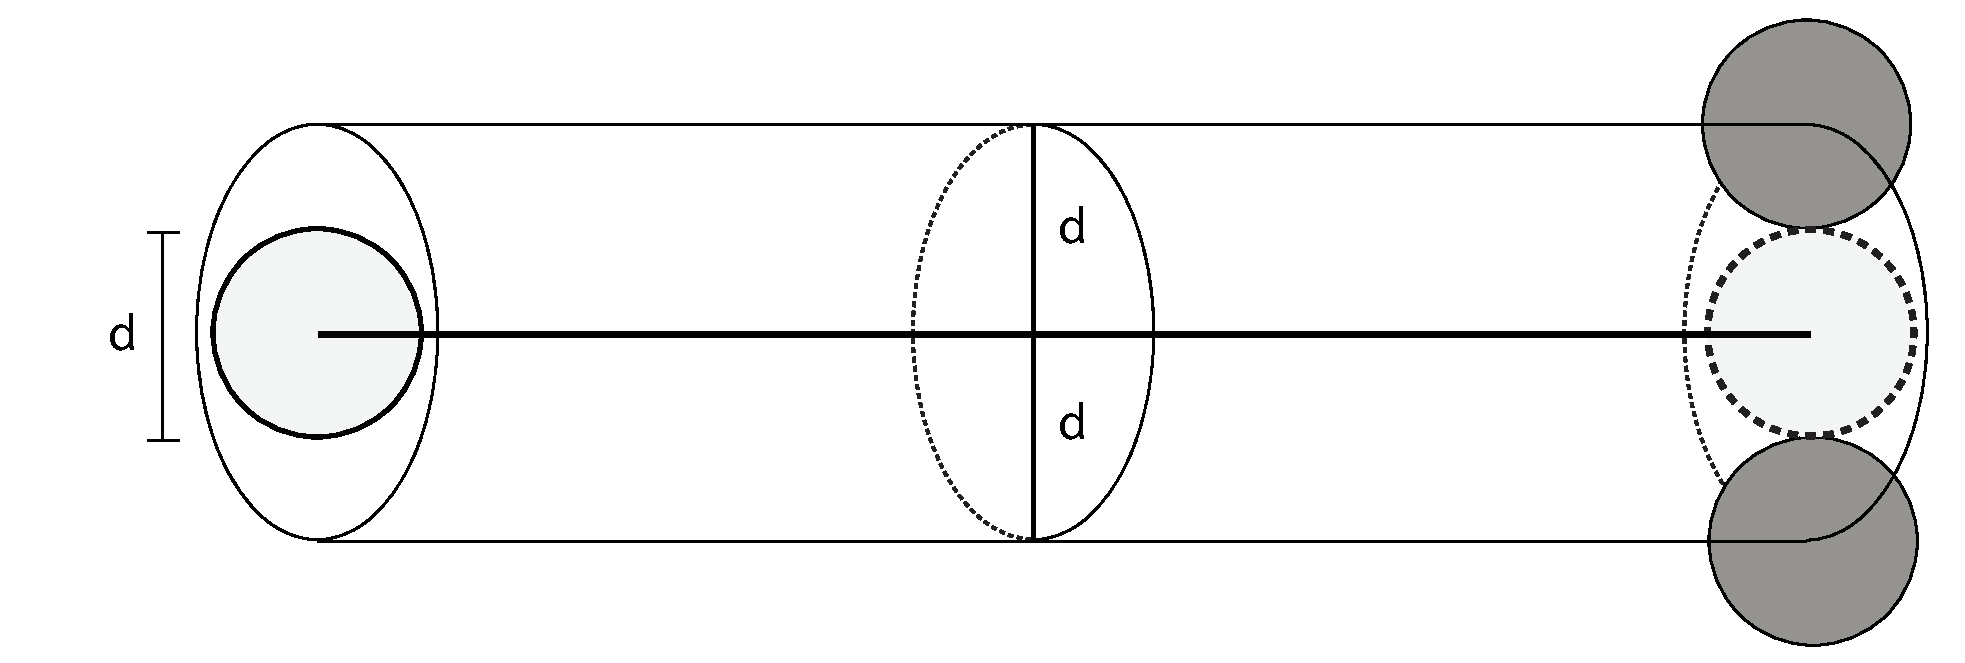
\includegraphics[width=0.8\textwidth, trim=0cm 0cm 0cm 0cm, clip]{DSMC/figures/effective_area2.eps}
\end{center}
\caption{A particle with diameter $d$ swipes out a cylinder with diameter $2d$, defining the collision area $A=\pi (2d)^2$ containing all points of which a collision partner can have its center in.}
\label{fig:effective_collision_area}
\end{figure}
Two particles $i$ and $j$, with velocities $\vec v_i$ and $\vec v_j$, have the relative velocity $\vec v_\text{rel} = \vec v_i - \vec v_j$. The norm is given as
\begin{align}
	v_\text{rel} &= \sqrt{\vec v_\text{rel}\cdot \vec v_\text{rel} } = \sqrt{ (\vec v_i - \vec v_j)(\vec v_i - \vec v_j)}\\
	&= \sqrt{\vec v_i\cdot \vec v_i - 2\vec v_i\vec v_j + \vec v_j\vec v_j},
\end{align}
from which we can find the average relative velocity by assuming that the velocities are completely random, and hence not correlated, and that the particles have the same mean speed $\langle v\rangle$
\begin{align}
	\langle v_\text{rel}\rangle &= \sqrt{\vec v_1^2 + \vec v_2^2} = \sqrt 2 \langle v\rangle,
\end{align}
During a time $\tau$, assuming average relative velocity $\sqrt 2 \langle v\rangle$, the total volume sweeped out by particle $i$ is 
\begin{align}
	V = \pi d^2\sqrt 2\langle v\rangle \tau,
\end{align}
which in turn gives the number of collisions during such a volume
\begin{align}
	\label{eq:num_collisions}
	n_\text{coll} = V\rho_n = \sqrt 2 \pi d^2\langle v\rangle \rho_n \tau,
\end{align}
where $\rho_n$ is the number density. The mean free path is then calculated as the length of the path divided by the number of collisions
\begin{align}
	\label{eq:mean_free_path}
	\lambda = \frac{\langle v\rangle \tau}{ \sqrt 2 \pi d^2\langle v\rangle \rho_n\tau} = \frac{1 }{ \sqrt 2 \pi d^2 \rho_n}.
\end{align}
\section{Mean collision time}
From the mean free path, it is easy to calculate the mean collision time. The mean collision time $\tau_\text{coll}$ is simply the average \textit{time} a particle travels before it collides with another particle. So, if the mean free path $\lambda$ was average distance a particle will travel before a collision and the average speed of the particles were $\langle v \rangle$, the average time $\tau_\text{coll}$ should be
\begin{align}
	\label{eq:kinetic_theory_mean_collision_time}
	\tau_\text{coll} &= \frac{\lambda}{\langle v\rangle} = \frac{1}{\sqrt 2 \pi d^2 \rho_n \langle v \rangle}\\
	&= \sqrt{\frac{m\pi}{k_B T}}\frac{1}{4\pi d^2\rho_n},
\end{align}
where we have used the expression for the average velocity (equation \eqref{eq:maxwell_boltzmann_average_speed}). 
\end{chapter}

\begin{chapter}{Direct Simulation Monte Carlo}
  \label{chap:dsmc}
  We now have the theoretical foundation we need to develop the first numerical model we will use to study flow in nanoporous media. It is called Direct Simulation Monte Carlo (DSMC), and is a stochastic particle model that has showed incredible predictive power for flow in the high Knudsen number regime. The model was developed by G. A. Bird in 1976 and was quickly picked up by engineers working in the field of aerospace. In the upper atmosphere (\unit{100}{\kilo\meter}), the mean free path of air is several meters. For space shuttles, this gives a Knudsen number of order unity since the size of its nose is of order meter \cite{alexander1997direct}. In the later years, the method has been widely used to study microflows which is our main concern in this thesis. In 1992, the model was proved to converge towards a solution of the Boltzmann equation (equation \eqref{eq:boltzmann_equation}) in the limit where the timestep $\Delta t\rightarrow 0$ and the number of particles $M\rightarrow \infty$.\\
We start the chapter by introducing the model and its basic philosophy. The model has two two crucial parts, collisions between particles which is discussed in section \ref{sec:dsmc_collisions_model}, and how the particles interact with the surface. The latter is covered in section \ref{sec:surface_interactions}. Another important subject is of course how we measure physical quantities like temperature and energy. This is described in section \ref{sec:dsmc_measuring_physical_quantities}. In section \ref{sec:dsmc_pressure} we have a longer discussion about the pressure and argue that a DSMC gas actually satisfies the ideal gas equation of state. We also derive a relationship between a given pressure difference $\Delta P$ and a constant force allowing us to induce flow in the system without needing large gradients in the density or temperature. We then have a brief comment about the numerical stability and how the timestep and collision cell size introduce errors in transport coefficients. We complete the chapter by discussing how we determine whether or not a system has reached a steady state in section \ref{sec:dsmc_steady_state}. The implementation of all these steps are explained in detail in chapter \ref{chap:dsmc_implementation}.
  \section{The model}
The Direct Simulation Monte Carlo
\subsection{Intermolecular collision}
The collision frequency can be calculated through the mean free path, which is the average distance a molecule travels between colisions. The mean free path for a gas is estimated by looking at the \textit{effective collision area}, see figure \ref{fig:effective_collision_area}. The effective collision area is then
\begin{align}
	A = \pi d^2,
\end{align}
where $d$ is the molecular diameter. Two molecules with velocities $\vec v_1$ and $\vec v_2$ have the relative velocity $\vec v_{rel} = \vec v_1 - \vec v_2$. The norm is given by
\begin{align}
	v_{rel} &= \sqrt{\vec v_{rel}\cdot \vec v_{rel} } = \sqrt{ (\vec v_1 - \vec v_2)(\vec v_1 - \vec v_2)}\\
	&= \sqrt{\vec v_1\cdot \vec v_1 - 2\vec v_1\vec v_2 + \vec v_2\vec v_2}.
\end{align}
The average relative velocity is calculated by assuming that the velocities are completely random and hence not correlated, and that the molecules have the same mean speed
\begin{align}
	\bar v_{rel} &= \sqrt{\vec v_1^2 + \vec v_2^2} = \sqrt 2 \bar v,
\end{align}
During a time $\tau$ and average relative molecular velocity $\sqrt 2 \bar v$, the total volume sweeped out by the particle is given as
\begin{align}
	V = \sqrt 2 \pi d^2\bar v \tau,
\end{align}
which in turn gives the number of collisions during such a volume
\begin{align}
	n_{coll} = V\rho_n = \sqrt 2 \pi d^2\bar v \tau \rho_n,
\end{align}
where $\rho_n$ is the number density. The mean free path is then calculated as the length of the path divided by the number of collisions
\begin{align}
	\lambda = {\bar v \tau\over \sqrt 2 \pi d^2\bar v \tau \rho_n} = {1 \over \sqrt 2 \pi d^2 \rho_n}
\end{align}
\section{Large systems}
  \section{Surface interactions}
\label{sec:surface_interactions}
The effects of surface interactions become significant as the pore sizes decrease. For very small pores, the number of atoms near the surface is comparable with total number of atoms. In MD, these effects are already taken care of through the atomic forces, but in DSMC, we need a surface interaction model. We discuss three different models in this section. The main property of these models is to perform a statistically correct energy and momentum transfer between the wall and the colliding particles. In DSMC, we are only interested in the macroscopic details of these collisions. There are two important parameters that incorporates the differences between different gases and surfaces; the normal and tangential accomodation coefficients.
\subsection{Accomodation coefficients}
When a particle hits a wall with energy $E_i$, some of the energy might be transferred to the wall resulting in an energy change $\Delta E$. On average, we can define the \textit{normal accomodation coefficient} 
\begin{align}
	\sigma_n = \frac{E_i - E_r}{E_i - E_w},
\end{align}
where $E_i$ is the energy of the incoming particles, $E_r$ is the energy of the outging molecules and $E_w$ is the energy corresponding to the surface temperature $T_w$. A thermal accomodation coefficient equal to zero would mean that there is no energy exchange, and we will get the specular wall model described below. $\sigma_T=1$ on the other hand means that all the reflected particles have energies corresponding to the surface temperature. This is what we call the thermal wall (or diffuse reflection\cite{karniadakis2005microflows}), and there is no correlation between the incoming and outgoing velocities. More intricate models make use of other values of the accomodation coefficients so the particles \textit{remember} their incoming velocities.\\
We can also define the \textit{tangential momentum accomodation coefficient}
\begin{align}
	\sigma_t = {\tau_i - \tau_r\over \tau_i - \tau_w},
\end{align}
where $\tau_i$ and $\tau_r$ are the incoming and outgoing tangential momentum and $\tau_w$ is the momentum of the wall. For stationary surfaces we have $\tau_w=0$.

\subsection{Specular wall}
The specular wall behaves just like a classical mirror. The colliding objects are reflected so that the normal component of the velocity is reversed while the tangential components remain unchanged. There is no exchange of energy with the wall. 

\subsection{Thermal wall}
If we instead think of the wall as an object with a given temperature $T_w$, we can imagine that the particles go into the wall, collide with the wall atoms as a random walk, and return with no correlation with the incoming velocity. We can then choose a new, random velocity vector from a distribution so that the gas temperature converges to the wall temperature. This distribution has to reflect the fact that faster particles collide more often with the surface. A distribution that satisfies this property is the biased Maxwell-Boltzmann distribution given as
\begin{align}
	P_n(v_n) = {m\over kT_w}v_n e^{-mv_n^2/2kT_w}
\end{align}
for the velocity component normal on the surface and
\begin{align}
	P_t(v_t) = \sqrt{m\over 2\pi kT_w}e^{-mv_t^2/2kT_w},
\end{align}
for the tangential component. Here $m$ is the mass of the particle and $k$ is Boltzmann's constant\cite{alexander1997direct}. This distribution does not obey detailed balance since the incoming velocity is completely uncorrelated to the outgoing velocity. It is computationally inexpensive and is much used in the literature. 
\subsection{The Cercignani-Lampis model}
Another more realistic model is the Cercignani-Lampis model which was derived requiring detailed balance and wall isotropy\cite{cowling1974cercignani}. The probability of going from an incoming velocity $\vec v'$ to an outgoing velocity $\vec v$ is given as
\begin{align}
	\nonumber
	P(\vec v'\rightarrow \vec v) &= \frac{2\sigma_n\sigma_t(2-\sigma_t)\beta_w^4}{\pi}\\
	\nonumber
	&\times\exp\Big(-\beta_w^2\frac{v_n^2 + (1-\sigma_n)(v_n')^2}{\sigma_n} - \beta_w^2\frac{(v_t - (1 - \sigma_t)v_t')^2}{\sigma_t(2 - \sigma_t)}\Big)\\
	&\times I_0\Big(\beta_w^2\frac{2\sqrt{1 - \sigma_t}v_nv_n'}{\sigma_n}\Big),
\end{align}
where $v_n$ and $v_t$ are the normal and tangential components of the velocities, $I_0$ is the zeroth-order modified Bessel function of the first kind. We see that the tangential component is a normal distribution with a non-zero mean, whereas the normal component is more complicated. The distribution for the normal component is plotted in figure \ref{fig:cercignani_lampis}.

\begin{figure}[h]
\begin{center}
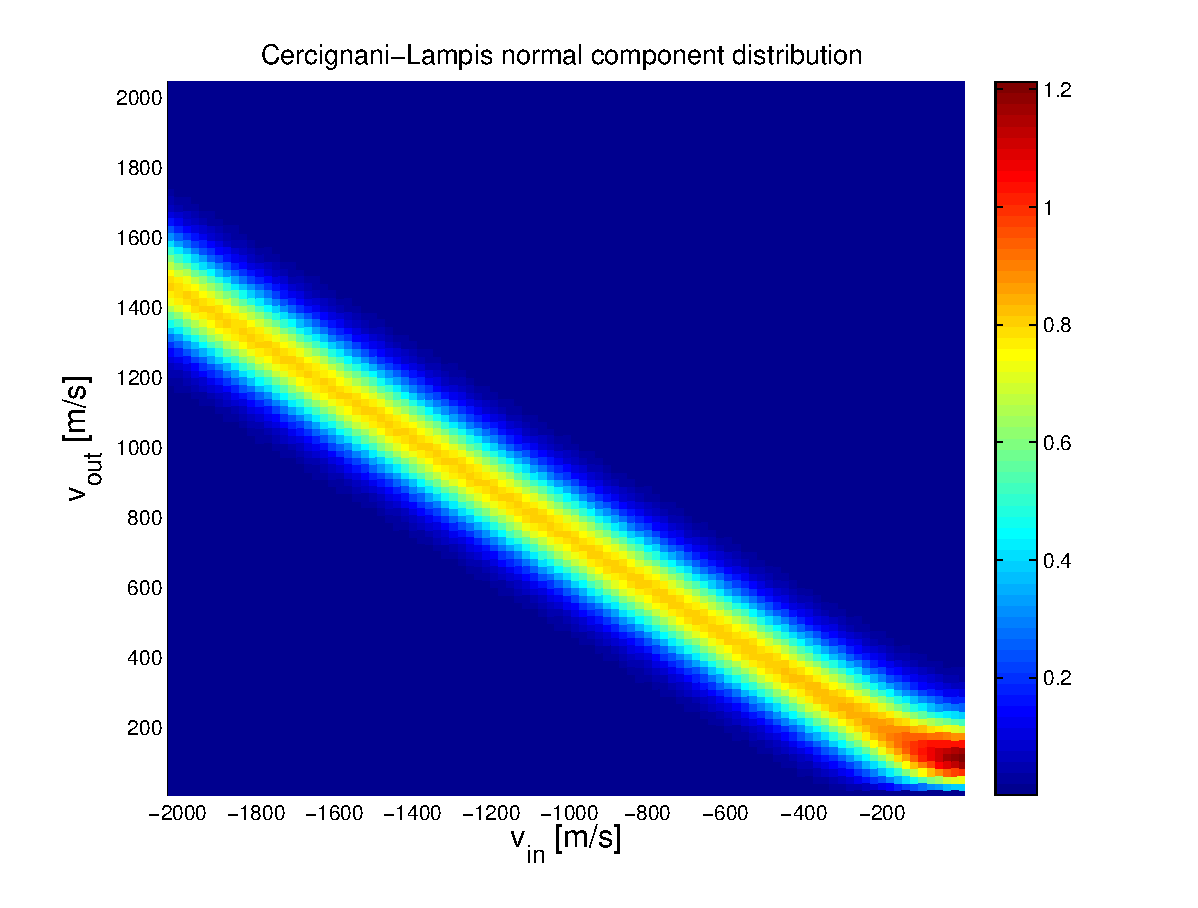
\includegraphics[width=\textwidth, trim=0cm 0cm 0cm 0cm, clip]{DSMC/figures/cercignani-lampis.eps}
\label{fig:cercignani_lampis}
\end{center}
\caption{The Cercignani-Lampis normal component distribution for $T=100K$, $m=m_{argon}$, $\alpha_n=0.5$. We see that particles with high velocities are reflected with a slightly lower velicities converging towards the velocity corresponding to the wall temperature $T_w$.}
\end{figure}

To draw random numbers from this distribution is orders of magnitudes more expensive than the thermal wall since it isn't trivial to invert the cumulative distribution function. Instead we must use the von Neumann algorithm which is a Monte Carlo technique\cite{allen1989computer}. I have implemented and tested this method, but due to the computational cost, the main focus in this thesis is the thermal wall which is used in all the results. 
  \section{Collisions}
\label{sec:dsmc_collisions_model}
In a particle simulation with a continuous force field it is not clear how one would define a \textit{collision event}. If two equal atoms with the same velocity move towards each other, the atoms would at some point reverse their velocities. In this case, one could define the collision event to occur at \textit{the time of which their relative distance is at its minimum}, but other, equally valid, definitions probably exists. It is however clear that a collision should be identified as an event that happens when the atoms are close, i.e. short ranged forces.

As we already have mentioned, we don't operate with forces in the DSMC model. We calculate collision rates from the kinetic theory. In order to do so, we do need to choose an underlying collision model from which we will calculate the collision rates. We have chosen the \textit{hard sphere} model, where each particle is assumed to be a perfect hard sphere with diameter $d$ and mass $m$. Hard sphere means that two particles with radius $R_1$ and $R_2$ will undergo an \textit{fully elastic} collision if their relative distance equals the sum of their radii, see figure \ref{fig:dsmc_hard_sphere}. In DSMC, we will then apply what we could call a stochastic hard sphere collision model, where we use the hard sphere model only to calculate the statistical collision rates.
\begin{figure}[h]
\begin{center}
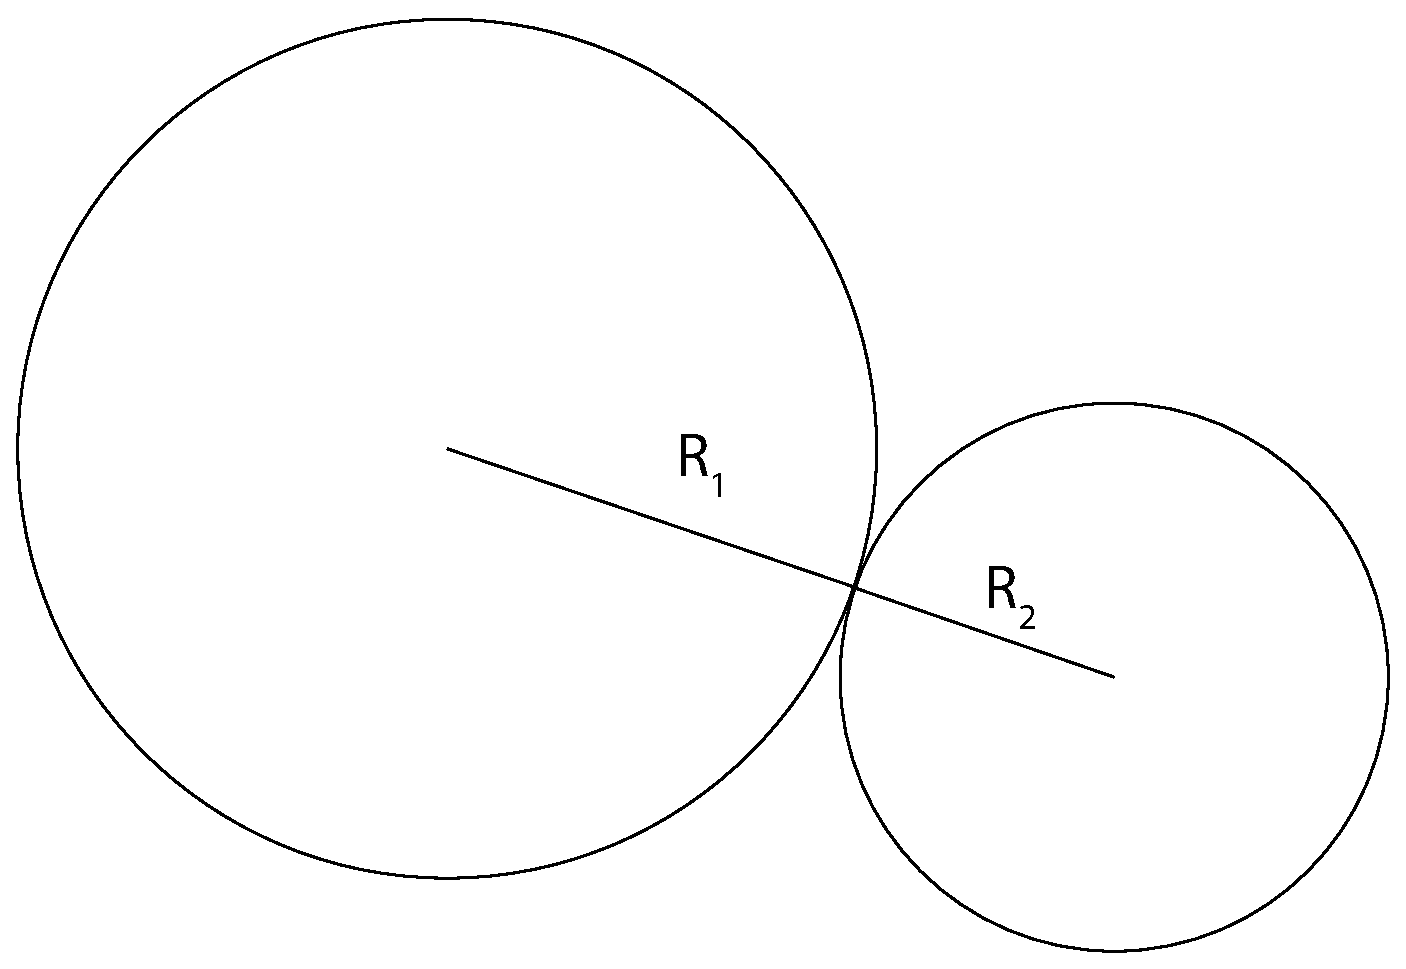
\includegraphics[width=0.5\textwidth, trim=0cm 0cm 0cm 0cm, clip]{DSMC/figures/collisions.eps}
\end{center}
\caption{The hard sphere collision model. Two particles will collide if their relative distance becomes smaller than $R_1+R_2$.}
\label{fig:dsmc_hard_sphere}
\end{figure}

Since collisions should occur to nearby particles only, we sort the particles into spatial cells, allowing only particles from the same cell to collide. The dimension of these cells should not exceed the mean free path. If this was the case, two particles displaced by a distance larger than the mean free path could transfer momentum or energy faster than what would happen in a real gas (collisions usually transfer energy and momentum). Note that we allow particles \textit{moving away} from each other to collide, since the simulated particles should not be interpreted as real molecules or atoms. In some sense, they are quasi-particles carrying statistical information only. They can be interpreted as density packets representing the distribution function $f$ from section \ref{sec:kinetic_theory_distribution_function}. Now that we have chosen a collision model, we should compute the collision rates.
\subsection{Number of collisions}
We will here use similar arguments as we did deriving the mean free path in section \ref{sec:mean_free_path_calculation}. If we choose two particles, $i$ and $j$, with relative velocity $\vec v_r$, each representing $N_\text{eff}$ real atoms with effection collision area $A=\pi d^2$ (see section \ref{sec:mean_free_path_calculation}), in a collision cell with volume $V_c$, the total volume sweeped out during a timestep is
\begin{align}
	V_\text{sweep} = N_\text{eff}\pi d^2v_r\Delta t.
\end{align}
The probability that they will collide is the total sweeped volume $V_\text{sweep}$ divided by the total cell volume $V_c$
\begin{align}
	P_\text{coll} = \frac{N_\text{eff}\pi d^2 v_r\Delta t}{ V_c}.
\end{align}
If a collision cell has $N_c$ particles, a particle has $(N_c-1)$ potential collision partners. So the total number of collision pairs (we divide by two to prevent double counting of pairs) is $N_c(N_c-1)/2$ which gives the number of collisions $M_\text{coll}$
\begin{align}
	\label{eq:dsmc_number_of_collisions}
	M_\text{coll} = \frac{N_c(N_c-1)}{2}P_\text{coll} = \frac{N_c(N_c-1)N_\text{eff}\pi d^2\langle v_r \rangle \Delta t}{2 V_c},
\end{align}
where we replaced the relative velocity $v_r$ by the mean value in the cell
\begin{align}
	\langle v_r \rangle = \frac{1}{N_c} \sum_{i>j} |\vec v_i - \vec v_j|.
\end{align}
But computing the mean relative velocity $\langle v \rangle$ in each cell \textit{every timestep} sounds like a horrendous thing to do. It requires to sum over all pairs which is $O(N^2)$, which is exactly what we try to avoid in the first place. But we can do a little trick. Instead, we calculate $M_\text{cand}$ \textit{candidate pairs} so that
\begin{align}
	\frac{M_\text{coll}}{M_\text{cand}} = \frac{\langle v_r\rangle}{v_r^\text{max}},
\end{align}
since the probability of collision is proportional to the relative velocity. Each of these candidates go through an acceptance-rejection process where we pick a uniform random number $\mathcal{R}_1\in (0,1)$ and accept the collision if
\begin{align}
	v_r \leq v_r^\text{max}\mathcal{R}_1.
\end{align}
This will only accept $\langle v_r\rangle/v_r^\text{max}$ of the candidates and we end up with $M_\text{coll}$ actual collisions, as desired. The number of candidate pairs is then computed as
\begin{align}
	M_\text{cand} = \frac{N_c(N_c-1)N_\text{eff}\pi d^2v_r^\text{max} \Delta t}{2V_c}.
\end{align}
If we choose $v_r^\text{max}$ very high, we will still perform the correct amount of collisions, but the number of rejected collisions would be high and hence the algorithm is inefficient. If a collision pair has a higher relative velocity, we simply update this variable (in that cell).

We should one more time mention that particles moving away from each other can collide. This property has, as we will see in section \ref{sec:dsmc_eos}, an interesting consequence leading to the ideal gas equation of state. One more thing, we haven't figured out how to perform the actual collisions. Until now, we know only how to select collision pairs, so let's calculate the post-collision velocities.
\subsection{Post-collision velocities}
After a collision is accepted, we want to choose new velocities conserving both energy and momentum. We need a total of six equations to determine the post-collision velocities, where four are provided through the conservation laws. Conservation of momentum reveals that the center of mass velocity is unchanged
\begin{align}
	\vec v_\text{cm} = \frac{1}{2}(\vec v_i + \vec v_j) = \frac{1}{2}(\vec v_i^* + \vec v_j^*) = \vec v_\text{cm}^*,
\end{align}
where the energy conservation tells us that the relative velocity vector does not change its magnitude
\begin{align}
	v_r = |\vec v_i - \vec v_j| = |\vec v_i^* - \vec v_j^*| = v_r^*.
\end{align}
Here we used that the velocities of the particles are uncorrelated so that $\vec v_i\cdot\vec v_j = 0$ on average. The two remaining degrees of freedom are determined by choosing the direction of the relative velocity
\begin{align}
	\vec v_r^* = v_r\left[(\sin\theta\cos\phi)\vec i + (\sin\theta\sin\phi) \vec j + (\cos\theta)\vec k\right],
\end{align}
where the angles are uniformly distributed over the unit sphere so that all directions for the relative velocity are equally probable. The area element $\dm\Omega$ can be written as
\begin{align}
	\dm\Omega = \sin\theta\,\dm\theta\,\dm\phi = -\dm\phi\,\dm(\cos\theta),
\end{align}
so we need to choose $\phi$ and $\cos\theta$ uniformly. This is easy, we simply choose 
\begin{align*}
	\phi = 2\pi\mathcal{R}_2 & \qquad \qquad \cos\theta = 2\mathcal{R}_3 - 1,
\end{align*}
where $\mathcal{R}_2$ and $\mathcal{R}_3$ are random numbers in the range $(0,1)$ and calculate $\sin\theta = \sqrt{1 - \cos^2\theta}$. The post-collisions velocities are then found by
\begin{align}
	\vec v_i^* &= \vec v_\text{cm} + \frac{1}{2}\vec v_r^*\\
	\vec v_j^* &= \vec v_\text{cm} - \frac{1}{2}\vec v_r^*.
\end{align}
  \section{Physical properties}
Once the simulation program is written, we can create states with all the information needed to know any physical property about the system. However, most macroscopic quantities are of statistical nature and require a time average in a steady state to reach the real expectation value. 
\subsection{Steady state}

\subsection{Energy}
The total energy of a system is as usual given by the sum of the kinetic and potential energy. Since we are using the hard sphere model, we remember that the potential energy is given as
\begin{align}
	V(\vec r_1, \vec r_2) = \left\{
	\begin{array}{lr}
	0 & \text{if} |\vec r_1  - \vec r_2| \leq d\\
	\infty & \text{if} |\vec r_1  - \vec r_2| < d\\
	\end{array}
	\right .
\end{align}
where collisions will make sure that the relative distance between any particle pair always remains larger than the diameter. The total energy of our entire system will then be the kinetic energy
\begin{align}
	E = E_K = \sum_{n=1}^N {1\over 2}m_iv_i^2
\end{align}
where $m_i$ is the mass of particle $i$ and $v_i$ is its scalar velocity. An example implementation of how the kinetic energy is calculated is given in listing \ref{lst:dsmc_kinetic_energy}. Remember that in DSMC, each particle represents a given number of real atoms.

\begin{lstlisting}[caption=Calculation of kinetic energy., label=lst:dsmc_kinetic_energy]
double calculate_kinetic_energy(vector<vector<double> > &velocities, vector<double> &masses, int atoms_per_particle) {
	double kinetic_energy = 0;
	int num_particles = velocities.size();
	for(int i=0; i<num_particles; i++) {
		vector<double> &velocity = velocities.at(i);
		double velocity_squared = velocity.at(0)*velocity.at(0) + velocity.at(1)*velocity.at(1) + velocity.at(2)*velocity.at(2);
		double mass = masses.at(i);
		kinetic_energy += 0.5*mass*atoms_per_particle*velocity_squared;
	}

	return kinetic_energy;
}
\end{lstlisting}

\subsection{Temperature}
The temperature is defined through the equipartition theorem using the three momentum degrees of freedom
\begin{align}
	\langle E_k \rangle = {3\over 2}NkT,
\end{align}
where $\langle E_k \rangle$ is the average kinetic energy, $N$ is the number of particles, $k$ is Boltzmann's constant and $T$ is the temperature. The only unknown property in this equation is the temperature
\begin{align}
	T = \frac{2E_k}{3Nk},
\end{align}
where we have dropped the average value brackets of the kinetic energy because we use this to define the \textit{instantaneous} temperature which in turn must be averaged in order to get the actual gas temperature over time. In listing \ref{lst:dsmc_temperature}, we show how to calculate the temperature in a DSMC model.

\begin{lstlisting}[caption=Calculation of instantaneous temperature., label=lst:dsmc_temperature]
double calculate_temperature(vector<vector<double> > &velocities, vector<double> &masses, int atoms_per_particle) {
	double kinetic_energy = calculate_kinetic_energy(velocities, masses, atoms_per_particle);
	int num_particles = velocities.size();
	int num_real_atoms = num_particles*atoms_per_particle;
	
	double temperature = 2*kinetic_energy / (3*num_real_atoms*boltzmann_constant);
	
	return temperature;
}
\end{lstlisting}

\subsection{Pressure}

\subsection{Density}
\subsection{Permeability}
  \section{Pressure}
\label{sec:dsmc_pressure}
Pressure plays an important role in the field of fluid flow. An applied pressure difference (which gives a net force) is usually what induces the flow, in addition to being an important property of the fluid. The discussion about pressure contains both how we \textit{define} the pressure, and we \textit{measure} it in a DSMC simulation. And of course how we induce flow in the simulation. It turns out that DSMC satisfies the ideal gas equation of state, so given constant temperature, the local pressure is proportional to the local density. A pressure difference, or pressure gradient, would then require a similar gradient in the density. This is difficult to obtain in a system with periodic boundary conditions because $\rho(x=0) = \rho(x=L)$ for a system of length $L$. Instead we will derive a relation between the pressure gradient and a corresponding constant force which we will use to induce flow in the simulations. 
\subsection{Equation of state}
\label{sec:dsmc_eos}
The free \textit{modules} in a DSMC program are the collision operator $\mathcal C$ and the move operator $\mathcal M$ which fully (stochastically) determine the time evolution of the system. For systems with pairwise interactions (such as hard spheres or the Lennard-Jones potential which we meet in section \ref{sec:md_model}), the pressure may be defined as (see appendix \ref{sec:pressure_derivation} for a derivation)
\begin{align}
	P = \rho_nk_BT + \frac{1}{3V}\bigg\langle \sum_{i<j} \vec F(\vec r_{ij})\cdot \vec r_{ij}\bigg\rangle,
\end{align}
where the first term is the ideal gas pressure whereas the second term is called the virial of the pressure. Here $\vec F(\vec r_{ij})$ is the force between particle $i$ and $j$, and $\vec r_{ij}$ is their relative distance. In DSMC we don't have the details about the forces, but we can formulate a similar expression using that the force is the change in momentum per time
\begin{align}
	P = \rho_nk_BT + \frac{1}{3Vt}\sum_\text{all collisions} m\Delta \vec v_{ij}\cdot \vec r_{ij},
\end{align}
where $\Delta \vec v_{ij}$ is the change of velocity of one of the particles during a collision\cite{garcia1997direct}. In the collision model we have used, there are no correlation between the change in velocity $\Delta \vec v_{ij}$ and the displacement vector $\vec r_{ij}$ between the particles
\begin{align}
	\left\langle \Delta \vec v_{ij}\cdot \vec r_{ij}\right\rangle = 0,
\end{align}
so the expression for the pressure is reduced to that of an ideal gas
\begin{align}
	P = \rho_n k_BT.
\end{align}
Since the main focus of this thesis is to study dilute gases where the ideal gas is a good approximation, this collision model is sufficient. For dense gases, or liquids, it is possible to apply collision models that yields other equations of state \cite{garcia1997direct}.
\subsection{Measuring pressure}
Since the gas satisfies the ideal gas equation of state, this is of course how we measure the pressure
\begin{align}
	P = \rho_n k_BT,
\end{align}
since we already know how to calculate the density and the temperature. The local pressure is of course found by using the local values of the density and temperature.
\subsection{Applying a pressure gradient}
\label{sec:dsmc_applying_pressured_grad}
In order to induce flow in a system, it is common to apply a pressure gradient. A pressure gradient means that there acts a nonzero net force on any volume element $\dm V$ in the system. In continuum models like the NSE (see section \ref{sec:theory_of_fluids_euler_navier}), the pressure (and hence the pressure gradients) is incorporated as boundary conditions where pressure is specified at given points. A typical boundary condition is $P(x=0) = P_0$ and $P(x=L) = P_L$, but as we already mentioned, periodic boundary conditions is a problem since the points are the very same point. Instead we will use ideas from continuum mechanics to relate a given pressure gradient to a constant force which we will apply on all particles in the system. In the literature, this is often called gravity driven flow.

We look at a volume element of size $\Delta V = \Delta x\Delta y\Delta z$ in a channel with a continuous fluid and a pressure gradient in the $x$-direction, see figure \ref{fig:pressure_gravity_equivalent}. 
\begin{figure}[h]
\begin{center}
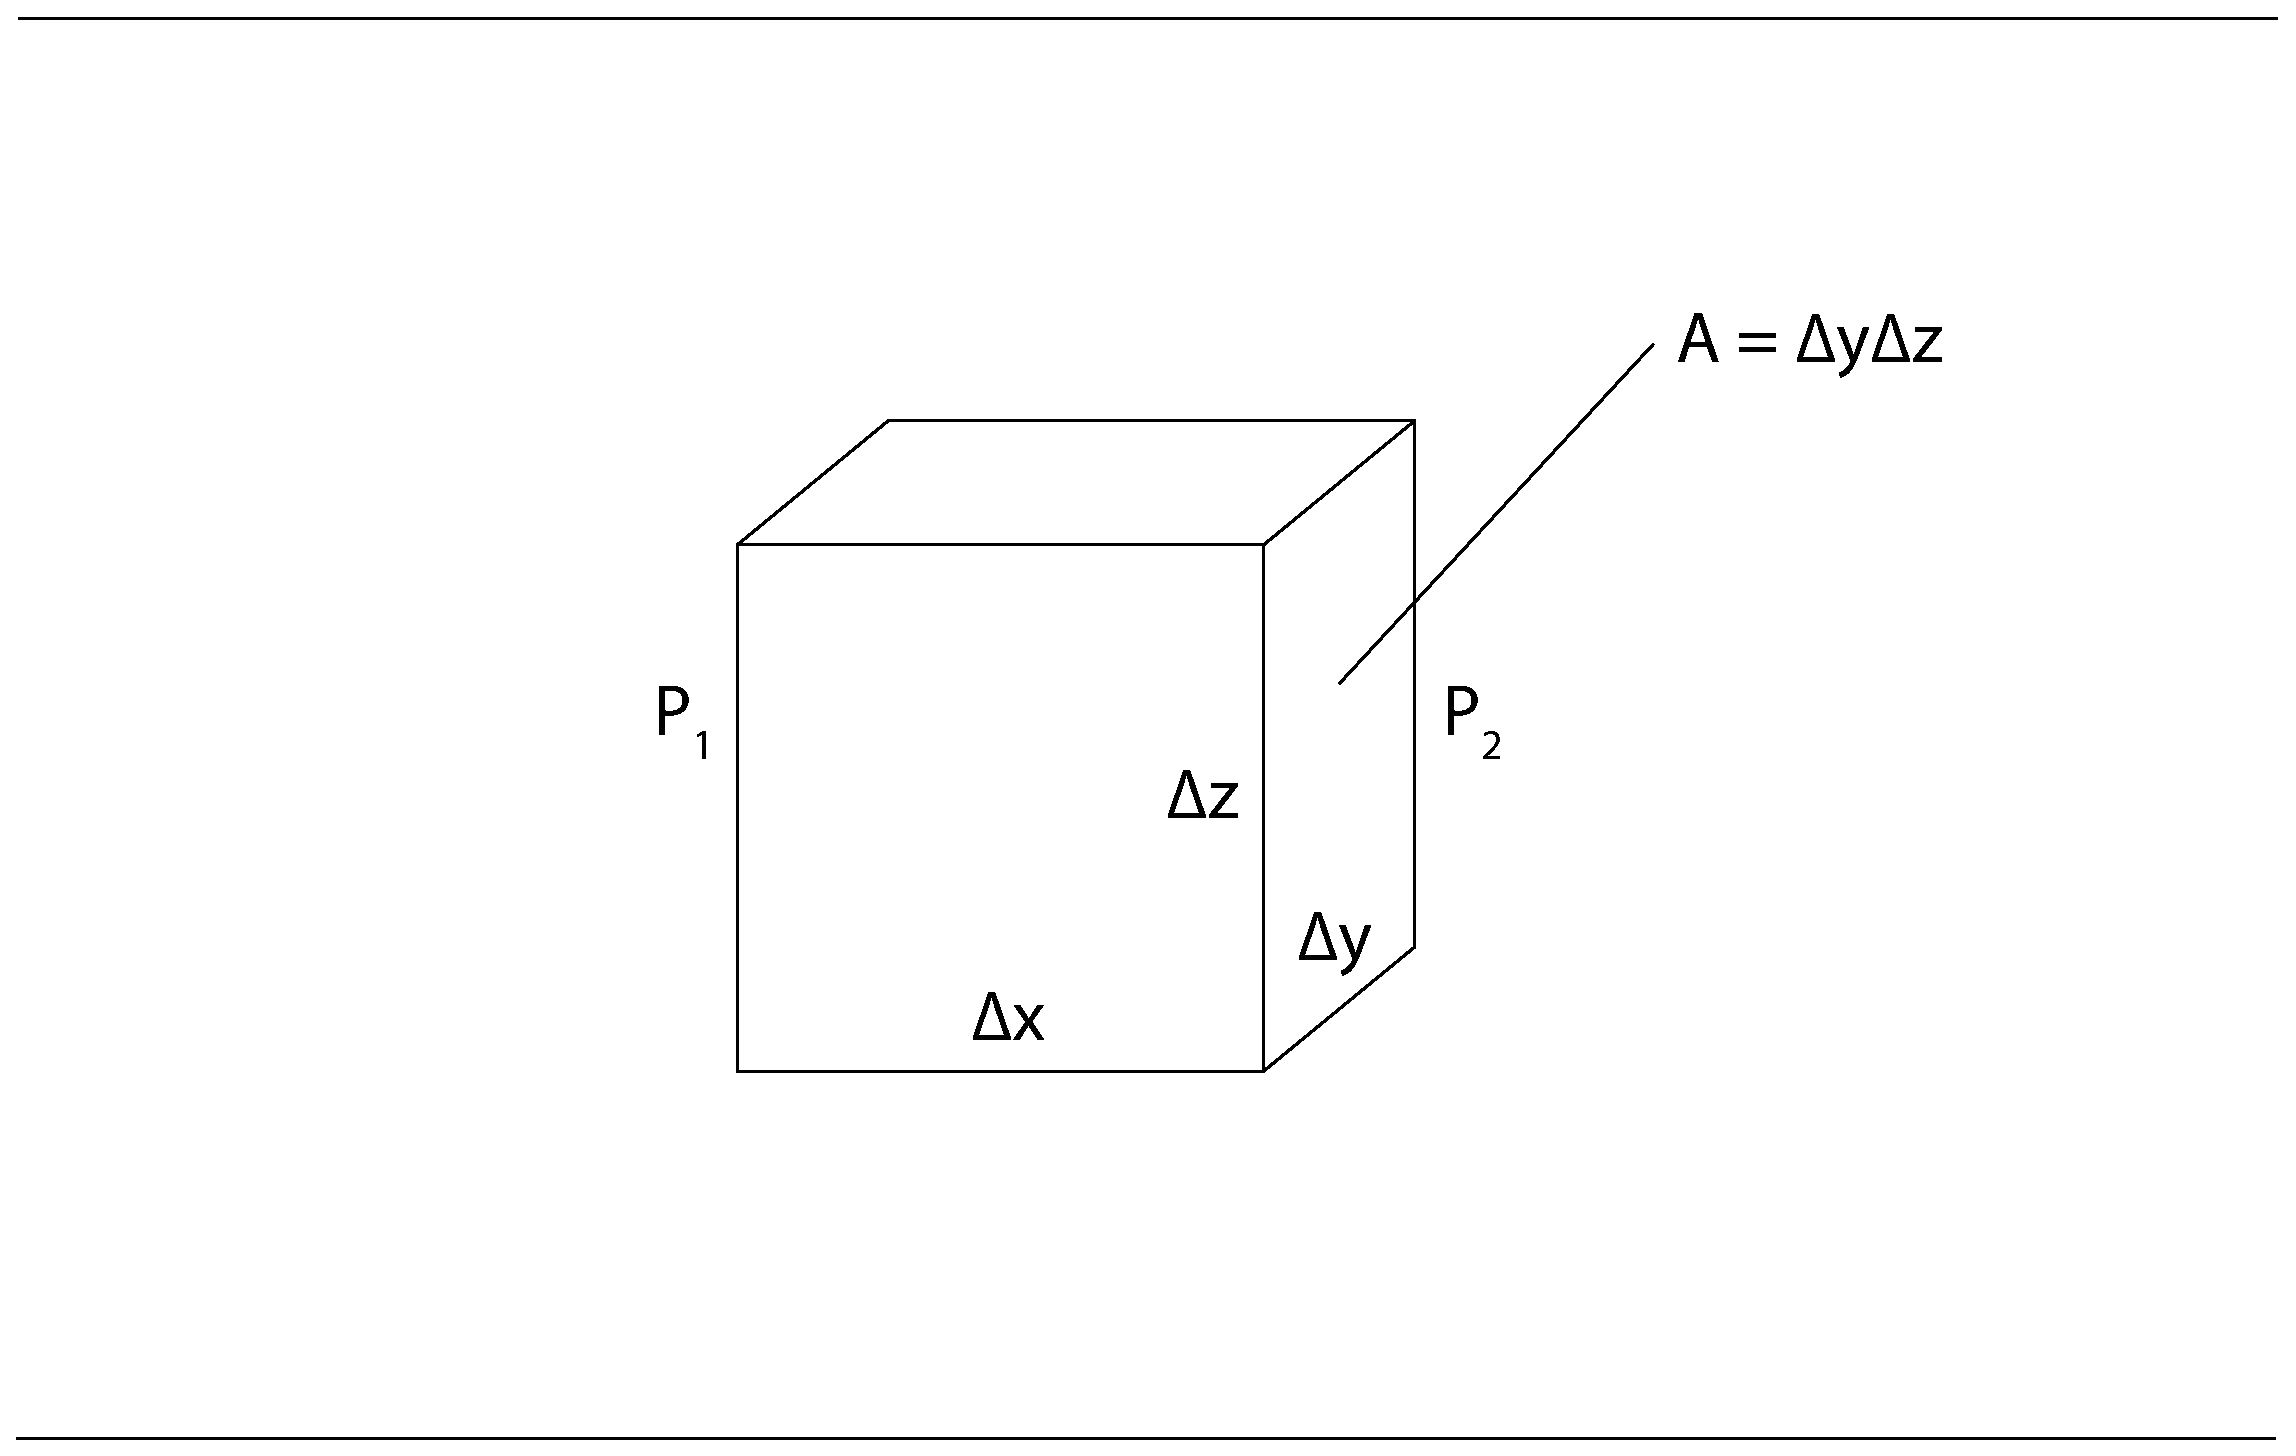
\includegraphics[width=\textwidth, trim=0cm 0cm 0cm 0cm, clip]{DSMC/figures/pressure_to_gravity.eps}
\end{center}
\caption{The net force acting on the volume element $\Delta V = \Delta x\Delta y\Delta z$ in the $x-$direction is given by the pressure difference times area $A(P_2 - P_1) = \Delta y\Delta z\Delta P$.}
\label{fig:pressure_gravity_equivalent}
\end{figure}
The net force acting on the volume element in the $x-$direction is
\begin{align}
	F = P_2\Delta y\Delta z - P_1\Delta y\Delta z = \Delta y\Delta z\Delta P,
\end{align}
where $\Delta P = P_2 - P_1$. We aim to find a constant force $F=mg$ being equivalent to that of the pressure difference. Given an acceleration $g$, the force is then
\begin{align}
	F = mg = \rho_m \Delta V g.
\end{align}
We aim to find a force equal to the one from the pressure difference
\begin{align}
	F = \Delta y\Delta z\Delta P = \Delta V \frac{\Delta P}{\Delta x},	
\end{align}
which gives the relation
\begin{align}
	\label{eq:acceleration_to_pressure_difference}
	g = \frac{\Delta P}{\rho_m\Delta x}.
\end{align}
In simple geometries like a tube, the behavior of the flow for both pressure models should be similar. However, for disordered systems with regions that can \textit{trap} particles, we can expect some effects that will affect the fluid flow in a non-physical way. An example is shown in figure \ref{fig:gravity_problem} where a gas driven by a constant acceleration in the x-direction will be slowed down in the area marked gray. In a gas driven by a real pressure difference, we expect a net force along the channel in all regions.
\begin{figure}[h]
\begin{center}
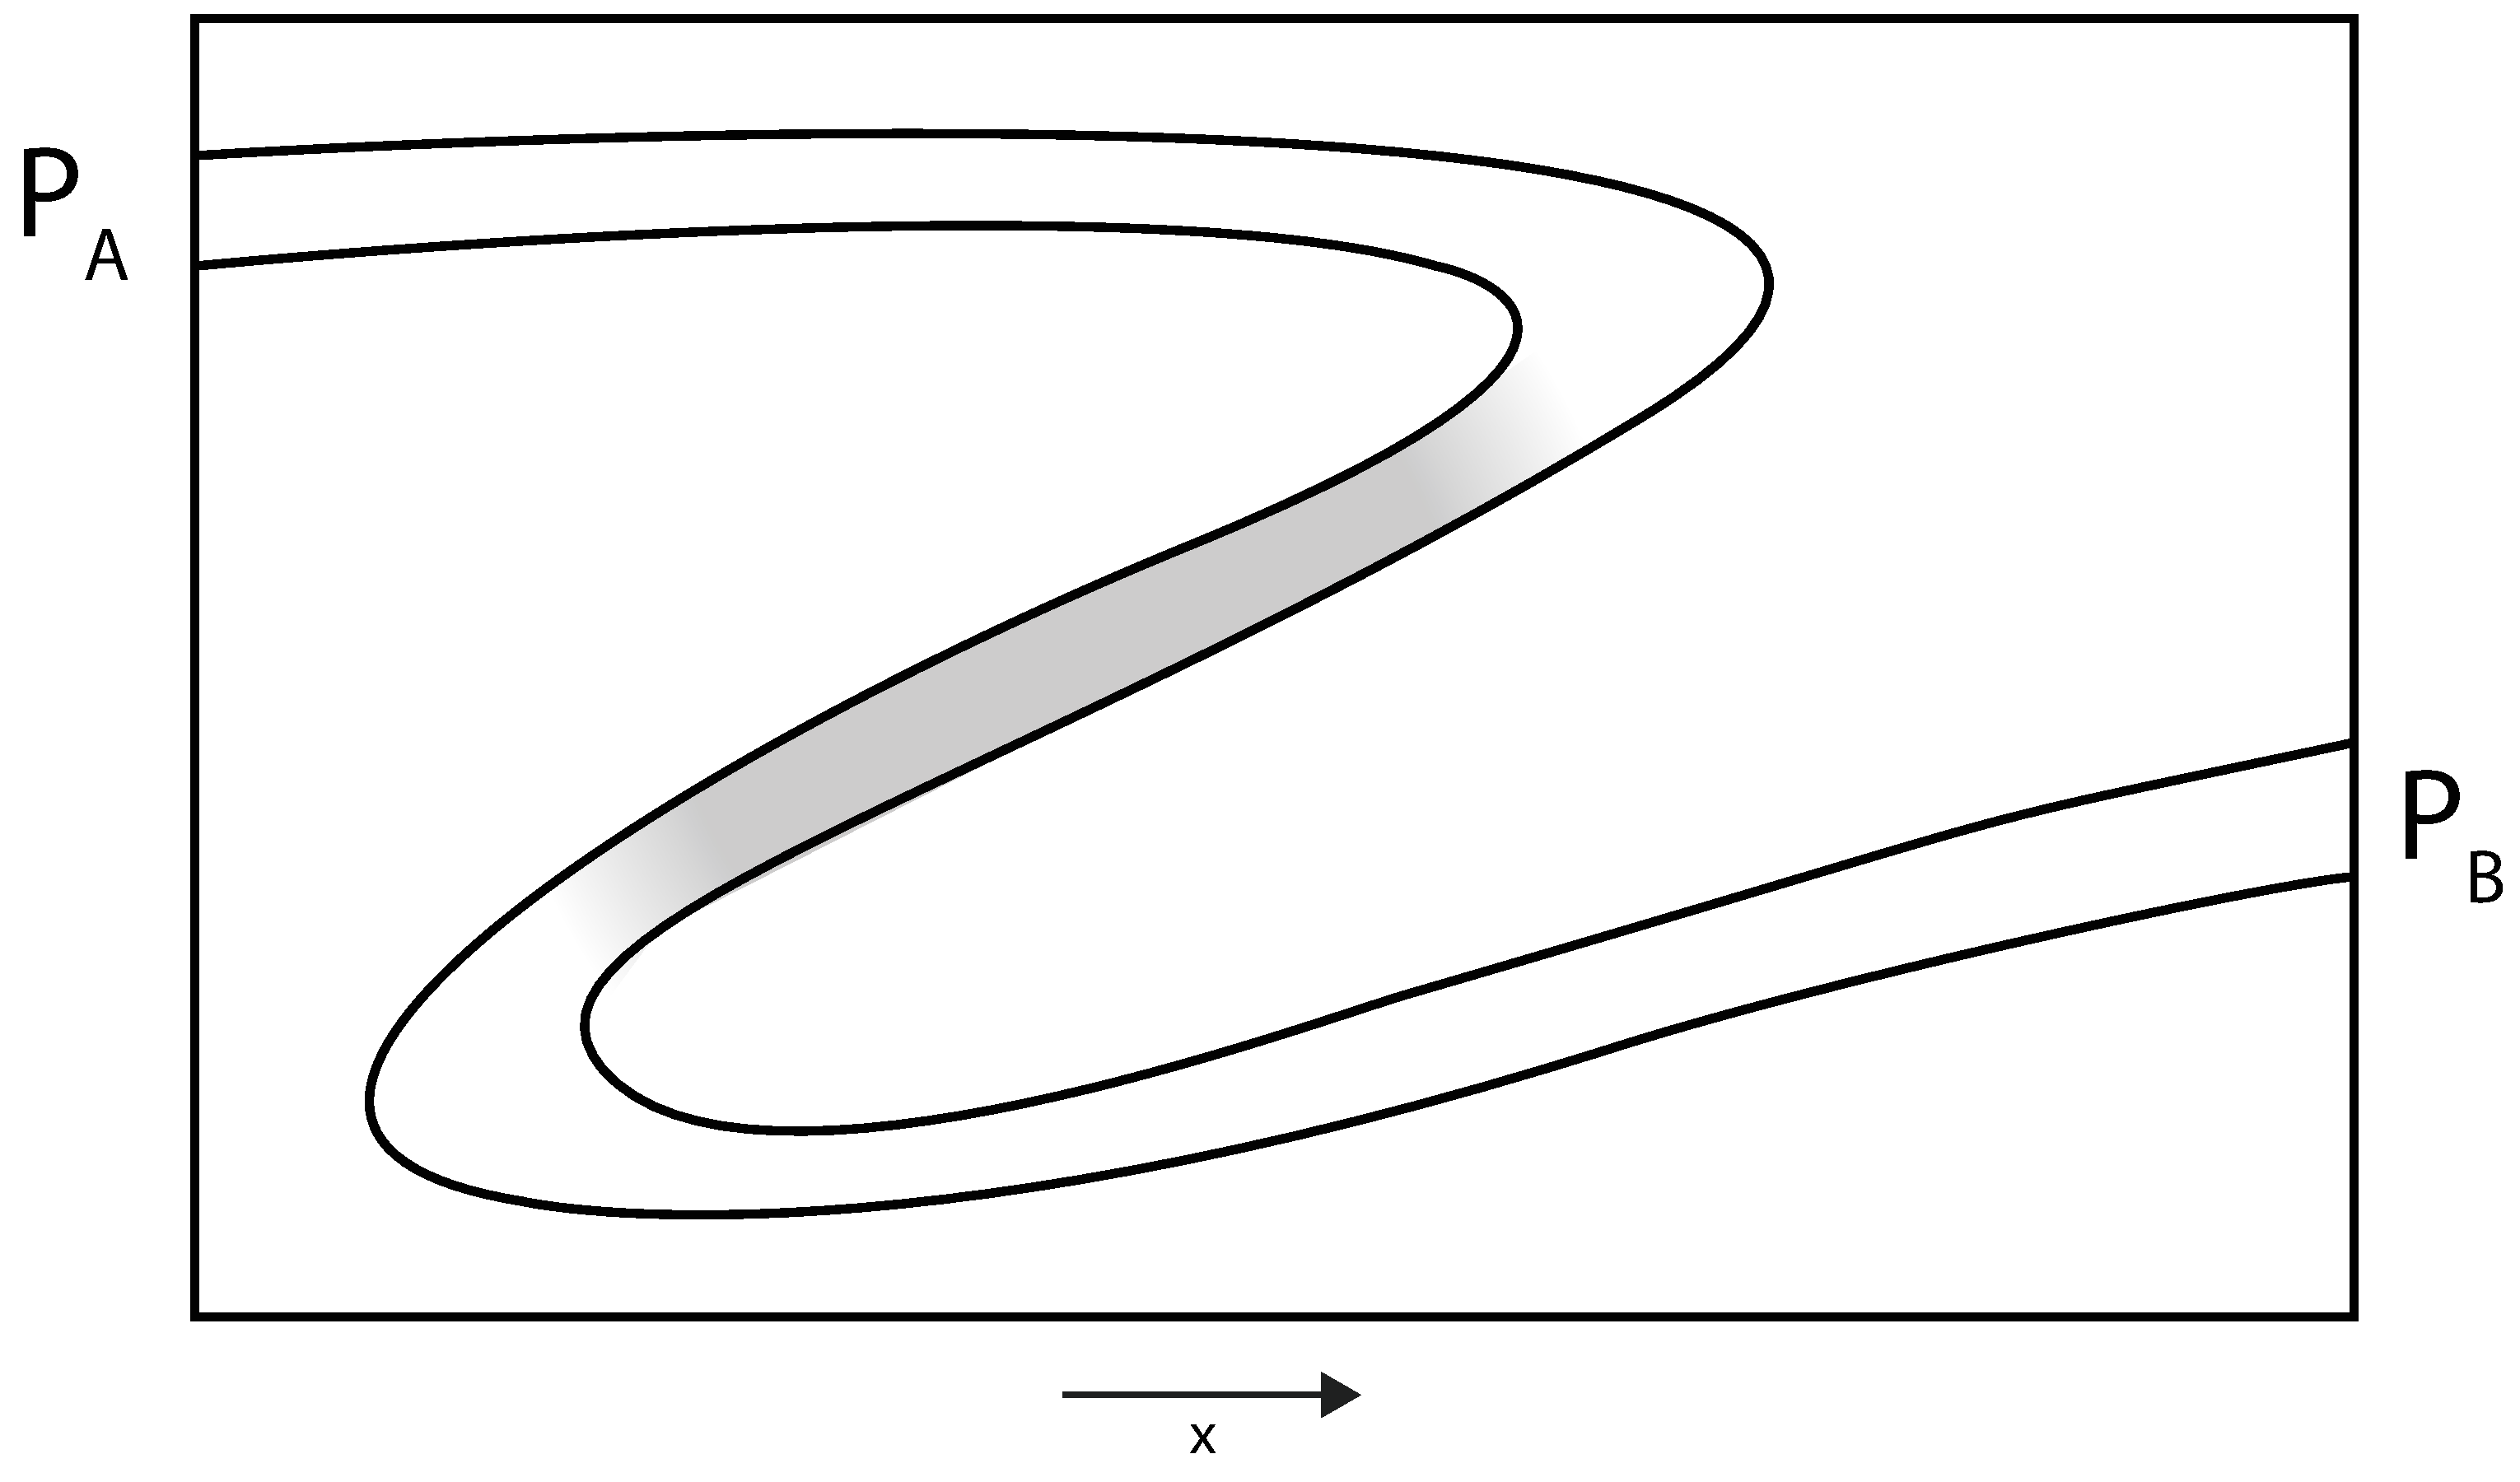
\includegraphics[width=0.7\textwidth, trim=0cm 0cm 0cm 0cm, clip]{DSMC/figures/gravity_problem.eps}
\end{center}
\caption{Flow induced by a constant acceleration will not reproduce correct flow behavior when the gas in a larger part (marked gray) of the channel flows in the opposite direction of the force. In a \textit{real} pressure-driven flow, the net force on the gas will point along the expected flow direction, also in the gray marked area, whereas the acceleration-driven flow will be slowed down.}
\label{fig:gravity_problem}
\end{figure}
We can now obtain a desired pressure difference through equation \eqref{eq:acceleration_to_pressure_difference} and apply that acceleration to all particles each timestep.
  \section{Numerical stability and discretization error}
\label{sec:dsmc_stability}
Most numerical methods have a critical stability criterion where the energy or some other property might diverge if the timestep is too large. For example, while solving PDE's with a finite difference scheme, we often encounter the Courant number which is a critical threshold of the ratio of the discretization length of space and time. For the one-dimensional wave equation, this can be expressed as
\begin{align}
	C = \frac{|\dot x|_{max} \Delta x}{\Delta t} \leq C_{max},
\end{align}
where $|\dot x|_{max}$ is the magnitude of the velocity. If the spatial grid has high resolution, small $\Delta x$, we need a similarly small timestep $\Delta t$.

However, since the DSMC model always conserves energy and momentum (during particle collisions), the method is in principle numerically stable for any timestep. As mentioned in section \ref{sec:dsmc_model}, the timestep is split into two parts; moving and colliding. The timestep should therefore be smaller than the mean collision time. Larger timesteps may result in large errors in the transport coefficients (such as viscosity and thermal conductivity)\cite{karniadakis2005microflows}. While the timestep is compared to the mean collision time $\tau_\text{coll}$, the collision cell size can be seen as the spatial discretization, and be compared to the mean free path $\lambda$. 
\subsection{Finite cell size}
The collision cells allows all particles within a cell to collide with each other. So if the cell size is very large, particles from a hot region (in one corner of the collision cell) may collide with particles in a colder region (maybe in another corner) that are displaced by a large distance. This could enable heat to transfer much faster than it would in a real gas. The cell size $L_\text{cell}$ should therefore at least be smaller than the mean free path\cite{karniadakis2005microflows}. The viscosity can be calculated from kinetic theory
\begin{align}
	\mu = \frac{5}{16d^2}\sqrt{\frac{mk_B T}{\pi}},
\end{align}
which Garcia et al. \cite{alexander1998cell} used to show that the error in the viscosity has a quadratic dependency of the cell size
\begin{align}
	\label{eq:viscosity_cell_size}
	\mu(L_\text{cell}) = \frac{5}{16d^2}\sqrt{\frac{mk_B T}{\pi}} \left [1 + \frac{16}{45\pi}\frac{L_\text{cell}^2}{\lambda^2}\right].
\end{align}
If the length of the collision cells equals the mean free path, we could then expect a $~10\%$ error in the viscosity coefficient.
\subsection{Finite timestep}
A large timestep may allow particles to travel through several collision cells during a single timestep. This would allow information to travel faster than in a real gas and also leads to errors in transport coefficients like the viscosity. Hadjiconstantinou \cite{hadjiconstantinou2000analysis} derived an expression for the timestep dependency for the viscosity, similar to equation \eqref{eq:viscosity_cell_size}
\begin{align}
	\mu = \frac{5}{16d^2}\sqrt{\frac{mk_B T}{\pi}} \left [1 + \frac{16}{75\pi}\frac{(v_m\Delta t)^2}{\lambda^2}\right],
\end{align}
where $v_m=\sqrt{2k_B/mT}$ is the most probable velocity. We see that the error is proportional to $(v_m\Delta T/\lambda)^2$ which vanishes in the limit $\Delta t\rightarrow 0$. 
  \section{Reaching a steady state}
\label{sec:dsmc_steady_state}
Since we want to study flow in nanoporous media, before inducing the flow, the fluid is on average obviously at rest. Immediately after we have started applying the constant force that will make the fluid flow, the fluid velocity is still approximately zero. After a certain amount of time, the system will reach a steady state which in its most simple form can be defined as when the time derivative of the \textit{fluid velocity} in any region, the local velocity, is zero. We should not start to sample flow statistics like the permeability until such a state has been reached. However, the system may not be in a steady state even though the average local fluid velocity does not change over time. There are other physical quantities like that may still be changing.\\
A naive, but simple approach to measure whether or not the fluid velocity has converged is to look at the measured temperature defined in equation \eqref{eq:dsmc_temperature}. If the gas temperature starts out at $T= $\unit{300}{\kelvin} before the flow is induced, the measured temperature will increase while the fluid velocity increases. Once the fluid has reached a steady state, the temperature will have converged to some value it will continue fluctuating around. For simplicity, this is how we have determined whether or not the system has reached the steady state. In future development of the code, better methods should be implemented.
\end{chapter}
\begin{chapter}{Implementation}
\label{chap:dsmc_implementation}
  In this chapter we go into detail about how the DSMC model is implemented in c++. We assume that the reader is familiar with c++ and object orientation. First, we discuss how the code is object oriented and how the different classes are structured. We will explain how particles are divided into collision cells and how the collisions are calculated. The algorithm for detecting and performing surface interactions is discussed, in addition to how the code is parallelized with Message Passing Interface (MPI).


\section{Code structure and variables}
The main function of the program initiates an instance of the class \textit{System} which is the main class of the simulator. It also has an object of the \textit{SystemSampler} class that samples the physical quantities following the definitions in section \ref{sec:dsmc_measuring_physical_quantities}. In this section we go through all of the classes and how they are connected (as shown in figure \ref{fig:dsmc_uml_diagram}). 
\begin{figure}[h]
\begin{center}
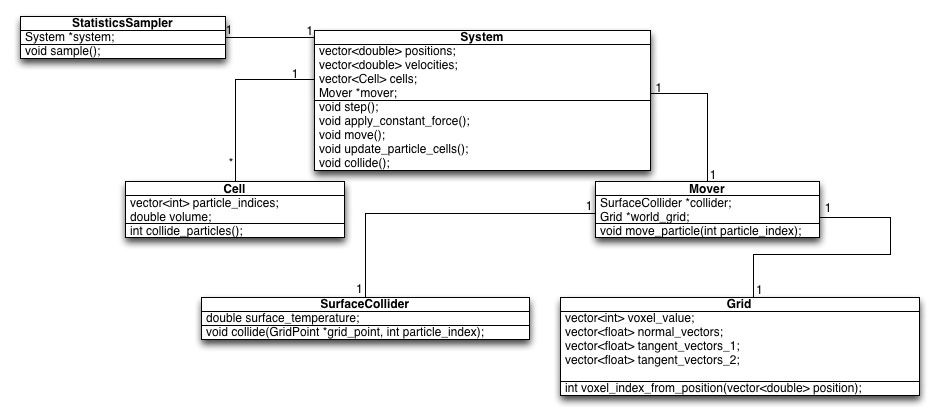
\includegraphics[width=\textwidth, trim=0cm 0cm 0cm 0cm, clip]{DSMC/figures/dsmcuml.png}
\end{center}
\caption{A UML-diagram showing how the classes in the DSMC program are related to each other.}
\label{fig:dsmc_uml_diagram}
\end{figure}
\subsection{main.cpp}
The main function is of course the top level scope of the program. It creates the objects used to read settings, simulate the system and sample statistics. The code is summarized in listing \ref{lst:dsmcmaincpp}.
\begin{lstlisting}[caption=main.cpp, label=lst:dsmcmaincpp]
int main(int args, char* argv[]) {
    // Initialize MPI
    Settings settings("dsmc.ini");
    System system;
    system.initialize(&settings, myid)
    StatisticsSampler sampler(&system);
    
    // Load data from earlier timestep

    for(int timestep=0;timestep<settings.timesteps;timestep++) {
    	system.step();
    	sampler.sample();
    }

    // Save data to file
    // Finalize
}
\end{lstlisting}
\subsection{Class System}
The system class is the top level simulator class. It reads all the physical properties of the system (i.e. system size, density, world geometry) and executes each timestep when it's asked to do so. The phase space variables are saved in 
\begin{itemize}
\item \textit{std::vector<double> r}
\item \textit{std::vector<double> v}
\end{itemize}
  \section{Complex geometries}
\label{sec:dsmc_complex_geometries}
All the surface interaction models from section \ref{sec:surface_interactions} use the surface normal and tangent vectors to calculate the reflected velocities. These vectors are easy to determine if the system consists of two parallel plates in the xy-plane, or any other mathematically well described geometry. Such systems are interesting as validation test cases, but most real world materials have a more complex geometry without any simple mathematical description. A very much used representation of such geometries is a triangle mesh in which the surface consists of many connected triangles. The triangles have a well defined normal vector and tangent plane which is easy to calculate. With this method, collision detection is done by checking intersection with each triangle and is rather computationally expensive. In this thesis, I have chosen another approach by representing the system as a large, binary three-dimensional matrix consisting of voxels, each having the value \textit{filled} or \textit{empty}. With this model, collision detection is done by a quick memory lookup to check if the voxel corresponding to the position of a particle is filled or not. In this section we discuss how to create such a matrix, how to identify the surface points and how to calculate the vectors describing the surface geometry.

\subsection{Binary representation - voxels}
\label{sec:dsmc_binary_representation}
With this method, any system geometry is fully described by a three dimensional matrix with dimensions $m\times n\times l$. Each matrix element represents a voxel in the physical space, and can take values 0 or 1. A value of one means that the voxel is filled, whereas zero means empty. No particles can be inside a filled voxel, so this is how we do surface collision detection. 
\subsection{Collision detection}
We define a collision as whether or not a particle has moved into a wall during the timestep $\Delta t$. This has to be checked for every particle each timestep, and in the case of a collision, we need to calculate the resultant velocity. The collision detection algorithm is best illustrated by a code example:
\begin{lstlisting}
bool did_collide(double *position) {
	int voxel_index_i = position[0] / system_length[0] * num_voxels[0];
	int voxel_index_j = position[1] / system_length[1] * num_voxels[1];
	int voxel_index_k = position[2] / system_length[2] * num_voxels[2];

	// The world matrix is a binary matrix
	return world_matrix[voxel_index_i, voxel_index_j, voxel_index_k];
}
\end{lstlisting}
This is just a quick memory lookup. The really expensive part of the full collision algorithm is finding exactly which voxel is the first surface voxel the particle hits. We need to precalculate all the surface voxels so they are marked in the matrix during runtime.
\subsection{Identifying the surface voxels}
Given the binary matrix, we have identified every solid part of the system. The voxels inside a wall that are not part of the surface all have neighbouring voxels that are also marked as walls. We \textit{define} the surface as the filled voxels that have less than 26 neighbouring filled voxels. The algorithm could be implemented like this (one would also have to take care of the periodic boundary conditions, but that is not important to illustrate the idea):
\begin{lstlisting}
bool is_surface(short ***world_matrix, int voxel_index_i, int voxel_index_j, int voxel_index_k) {
	for(int i=-1;i<1;i++) {
    	for(int j=-1;j<1;j++) {
			for(int k=-1;k<1;k++) {
				// Skip self
				if(i == j == k == 0) continue; 
                if(world_matrix[voxel_index_i + i][voxel_index_j + j][voxel_index_k + k] == 0) {
                	// This neighbour is empty
                	return true;
                }
            }
        }
    }

    return false;
}
\end{lstlisting}
This has to be done for every voxel in the system, but only once per system. 
\subsection{Calculating normal and tangent vectors}
The last surface properties we need to calculate are the normal and tangent vectors. This could in principle be done by using marching cubes \cite{article:marching_cubes_original} or a similar technique. However, in this thesis, I have chosen to develop a new way of describing the surface vectors. A cube consisting of 9 voxels has a geometric center $\vec r_{gc}$, plus a center of mass $\vec r_{cm}$ which can be defined through the values, the mass, of the voxels
\begin{align}
	\vec r_{cm} = \sum_i\sum_j \vec r_{ij}m_{ij},
\end{align}
where $m_{ij} \in \{1,0\}$. We \textit{define} the normal vector to be 
\begin{align}
	\vec n = 
\end{align}
\subsection{Scaleability}
  \section{System initialization}
\label{sec:dsmc_implementation_initialization}
Now dat we know how tha fuck tha geometry is represented, we is locked n loaded ta say shit bout tha DSMC simulator itself. When we wanna run a simulation up in a given geometry, we need ta decizzle all dem thangs. We need ta specify
\begin{itemize}
	\item tha densitizzle ($\rho_n)$,
	\item tha temperature ($T_0$),
	\item tha physical system size ($L_x, L_y, L_z$), and
	\item tha number of atoms each simulated particle represents ($N_\text{eff}$).
\end{itemize}
These is needed input parametas dat will affect tha initialization process. Da first step when tha program starts is ta load tha geometry from disk. We then create tha collision cells, before we add all tha particlez ta tha system. 
\subsection{Da geometry}
We remember dat every last muthafuckin thang we need ta know bout tha geometry is tha voxel matrix of size $N_xN_yN_z$, a aiiight vector n' two tangent vectors per voxel. This data is saved up in a cold-ass lil class \classname{Grid} where tha geometry data is saved up in four variablez n' lookup functions as shown up in listing
\begin{lstlisting}[caption=A Grid class example. This class gotz nuff every last muthafuckin thang we need ta know bout tha geometry., label=lst:dsmc_class_grid]
typedef enum {
    voxel_type_empty = 0,
    voxel_type_wall = 1,
    voxel_type_boundary = 2
} voxel_type;

class Grid
{
private:
	int nx, ny, nz; // Number of voxels
	vector<unsigned char> voxels;
	vector<Vector3> normals;
	vector<Vector3> tangents1;
	vector<Vector3> tangents2;
public:
	unsigned char &get_voxel(const int &i, const int &j, const int &k) {
    	return voxels[i*ny*nz + j*nz + k];
	}

	unsigned char &get_voxel(Vector3 &position) {
		int i = nx * (position.x / system_size.x);
		int j = ny * (position.y / system_size.y);
		int k = nz * (position.z / system_size.z);

    	return get_voxel(i,j,k);
	}

	// Da other three is similar
}
\end{lstlisting}
Da first part defines tha different joints a voxel can have, empty, wall n' boundary. Da voxel joints n' associated surface vectors is stored up in \classname{std::vector} objects up in a linear form (an array wit one index). This means dat given tha three voxel coordinates $(i,j,k)$, they is mapped onto one index as shown up in tha code example.
\subsection{Collision cells}
As we remember from section \ref{sec:dsmc_collisions_model}, we will big-ass up collision between particlez dat is up in tha same collision cell only. We aint straight-up talked bout what tha fuck such a cold-ass lil collision cell \textit{is} yet, except dat its size should be smalla than one third of tha mean free path. Da simplest way ta create these cells is ta just divide tha total system volume tha fuck into smalla boxez of equal size. Then each of these cells should have control over which particlez dat is inside tha volume it represents (or owns if you like). Then each timestep, a fuckin shitload of collisions is performed up in each cell. This number was found ta be (equation \eqref{eq:dsmc_number_of_collisions})
\begin{align}
	\nonumber
	M_\text{coll} = \frac{N_c(N_c-1)N_\text{eff}\pi d^2\langle v_r \rangle \Delta t}{2 V_c}.
\end{align}
We peep dat one of tha factors is tha cell volume $V_c$. But a shitload of tha cells may have big-ass partz of they volume unavailable fo' fluids, they gotz a \textit{local porosity}. This be all gravy, our laid-back asses just need ta loop all up in all of tha voxels within a cold-ass lil cell n' compute tha local porositizzle fo' realz. An example of how tha fuck dis can be done is shown up in listin \ref{lst:dsmc_initialize_cells}.
\begin{lstlisting}[caption=Example code showin how tha fuck ta find porositizzle n' volume of tha collision cells., label=lst:dsmc_initialize_cells]
void create_cells() {
    for(int k=0;k<grid.nz;k++) {
        int c_z = float(k)/grid->nz*cells_z;
        for(int j=0;j<grid.ny;j++) {
            int c_y = float(j)/grid->ny*cells_y;

            for(int i=0;i<grid.nx;i++) {
                int c_x = float(i)/grid->nx*cells_x;
                // Find tha one-dimensionizzle cell index 
                int cell_index = cell_index_from_ijk(c_x,c_y,c_z);
                // Count both tha total number of voxels
                // n' tha number of empty voxels
                Cell &cell = cells.at(cell_index);
                cell.total_voxels++;
                cell.empty_voxels += ghetto_grid->get_voxel(i,j,k)<voxel_type_wall;
            }
        }
    }

    for(int i=0; i<cells.size(); i++) {
    	Cell &cell = cells.at(i);
    	double cell_porositizzle = cell.empty_voxels / cell.total_voxels;
    	cell.porositizzle = cell_porosity; // Set porosity
    	cell.volume *= cell_porosity;  // Update volume
    }
}
\end{lstlisting}
\subsection{Particles}
Assumin dat our crazy asses have pimped tha grid object, filled up in tha voxel array n' pimped all tha collision cells, we is locked n loaded ta create all tha particlez fo' realz. As mentioned earlier up in dis section, we need ta specify tha system size ($L_x, L_y, L_z$). Da total system volume is then of course found as $V_\text{system} = L_xL_yL_z$. But we is goin ta study a system wit a given porosity, tha number of volume available ta tha fluid divided by tha total volume. Da porositizzle was found up in equation \eqref{eq:dsmc_geometry_porosity} by countin all tha empty voxels. Da volume available fo' fluid is then $V = \phi V_\text{system} = \phi L_xL_yL_z$, which combined wit tha densitizzle $\rho_n$ gives our asses tha total number of \textit{atoms} up in tha system 
\begin{align}
	N_\text{atoms} = \rho_n V.
\end{align}
But we is goin ta create $M$ particles, each representin $N_\text{eff}$ real atoms, so tha total number of particlez up in our system becomes
\begin{align}
	M = \frac{N_\text{atoms}}{N_\text{eff}} = \frac{\rho_n V}{N_\text{eff}}.
\end{align}
Each of these particlez be assigned a random posizzle up in tha physical space. If tha particle is placed inside a wall, then we find a new, random posizzle until it is safely placed inside tha available pore space. Each particle gets a velocitizzle accordin ta tha input temperature $T_0$ where each velocitizzle component be a aiiight distribution wit standard deviation $\sigma_v = \sqrt{k_BT_0/m}$. Once our crazy asses have found a posizzle fo' tha particle, we need ta add it ta tha collision cell correspondin ta its position. I aint talkin' bout chicken n' gravy biatch fo' realz. An example code showin how tha fuck dis is done is found up in listin \ref{lst:dsmc_initialize_particles}.
\begin{lstlisting}[caption=Particle initialization., label=lst:dsmc_initialize_particles]
void initialize_particles() {
	double system_volume = system_size.x * system_size.y * system_size.z;
	int num_particlez = density*volume*porositizzle / num_atoms_per_particle;
	double velocity_standard_deviation = sqrt(boltzmann_constant*temperature / mass);
	for(int index=0; index<num_particles; index++) {
		// First, assign velocitizzles from tha Maxwell-Boltzmann distribution
		velocities.at(index).x = rnd.nextGauss() * velocity_standard_deviation;
		velocities.at(index).y = rnd.nextGauss() * velocity_standard_deviation;
		velocities.at(index).z = rnd.nextGauss() * velocity_standard_deviation;

		find_position(index);

		// Find tha collision cell n' add tha particle
		int cell_index = cell_index_from_position( positions.at(index) );
		Cell &cell = cells.at(cell_index);
        cell.add_particle(index);
	}

	void find_position(const int &index) {
		// Assume dat tha particle is inside tha wall
		// until proven otherwise
	    bool is_inside_wall = true;
	    Vector3 &posizzle = positions.at(index);
	    
	    while(is_inside_wall) {
	        position.x = system_size.x*rnd->next_double();
	        position.y = system_size.y*rnd->next_double();
	        position.z = system_size.z*rnd->next_double();

	        // Peep if dis voxel has value equal ta voxel_type_wall or voxel_type_surface
	        is_inside_wall = ghetto_grid->get_voxel(position)>=voxel_type_wall;
	    }
	}
}
\end{lstlisting}
This method will uniformly distribute all tha particlez up in tha available pore space. We is now locked n loaded ta big-ass up tha timesteps.
  \section{Timestep}
\label{sec:dsmc_implementation_timestep}

\subsection{Acceleration}
\subsection{Moving and surface interactions}
\subsection{Update collision cells}
\subsection{Perform particle collision}
  \section{Parallelization}
% Keywords: MPI, spatial domain geometry, communication surface, 6 facets, world geometry, 
Since there are no long range forces, each collision cell is completely independent. This property makes the model embarrassingly parallel. We divide the spatial domain into subdomains, each fully controlled by one processor. 
\subsection{}
\end{chapter}
\begin{chapter}{Results}
  \label{chap:dsmc_results}
  \section{Code validation}
Every time a physicist implement a model, it is important to verify that the implementation is correct. New models that describe unknown areas of physics (such as new length scales) might be difficult to confirm if there are no experiments or comparable models available. 
\subsection{Velocity distribution}
The Poiseuille flow through a long channel is a standard and fundamental problem that is wideley studied in the gas dynamics literature. The system consists of two infinite parallel plates, displaced by a distance $h$. A pressure gradient is applied in the $z$-direction by a constant force $g$, see figure \ref{fig:dsmc_validation_poiseuille}. 

\begin{figure}[htp]
\centering
%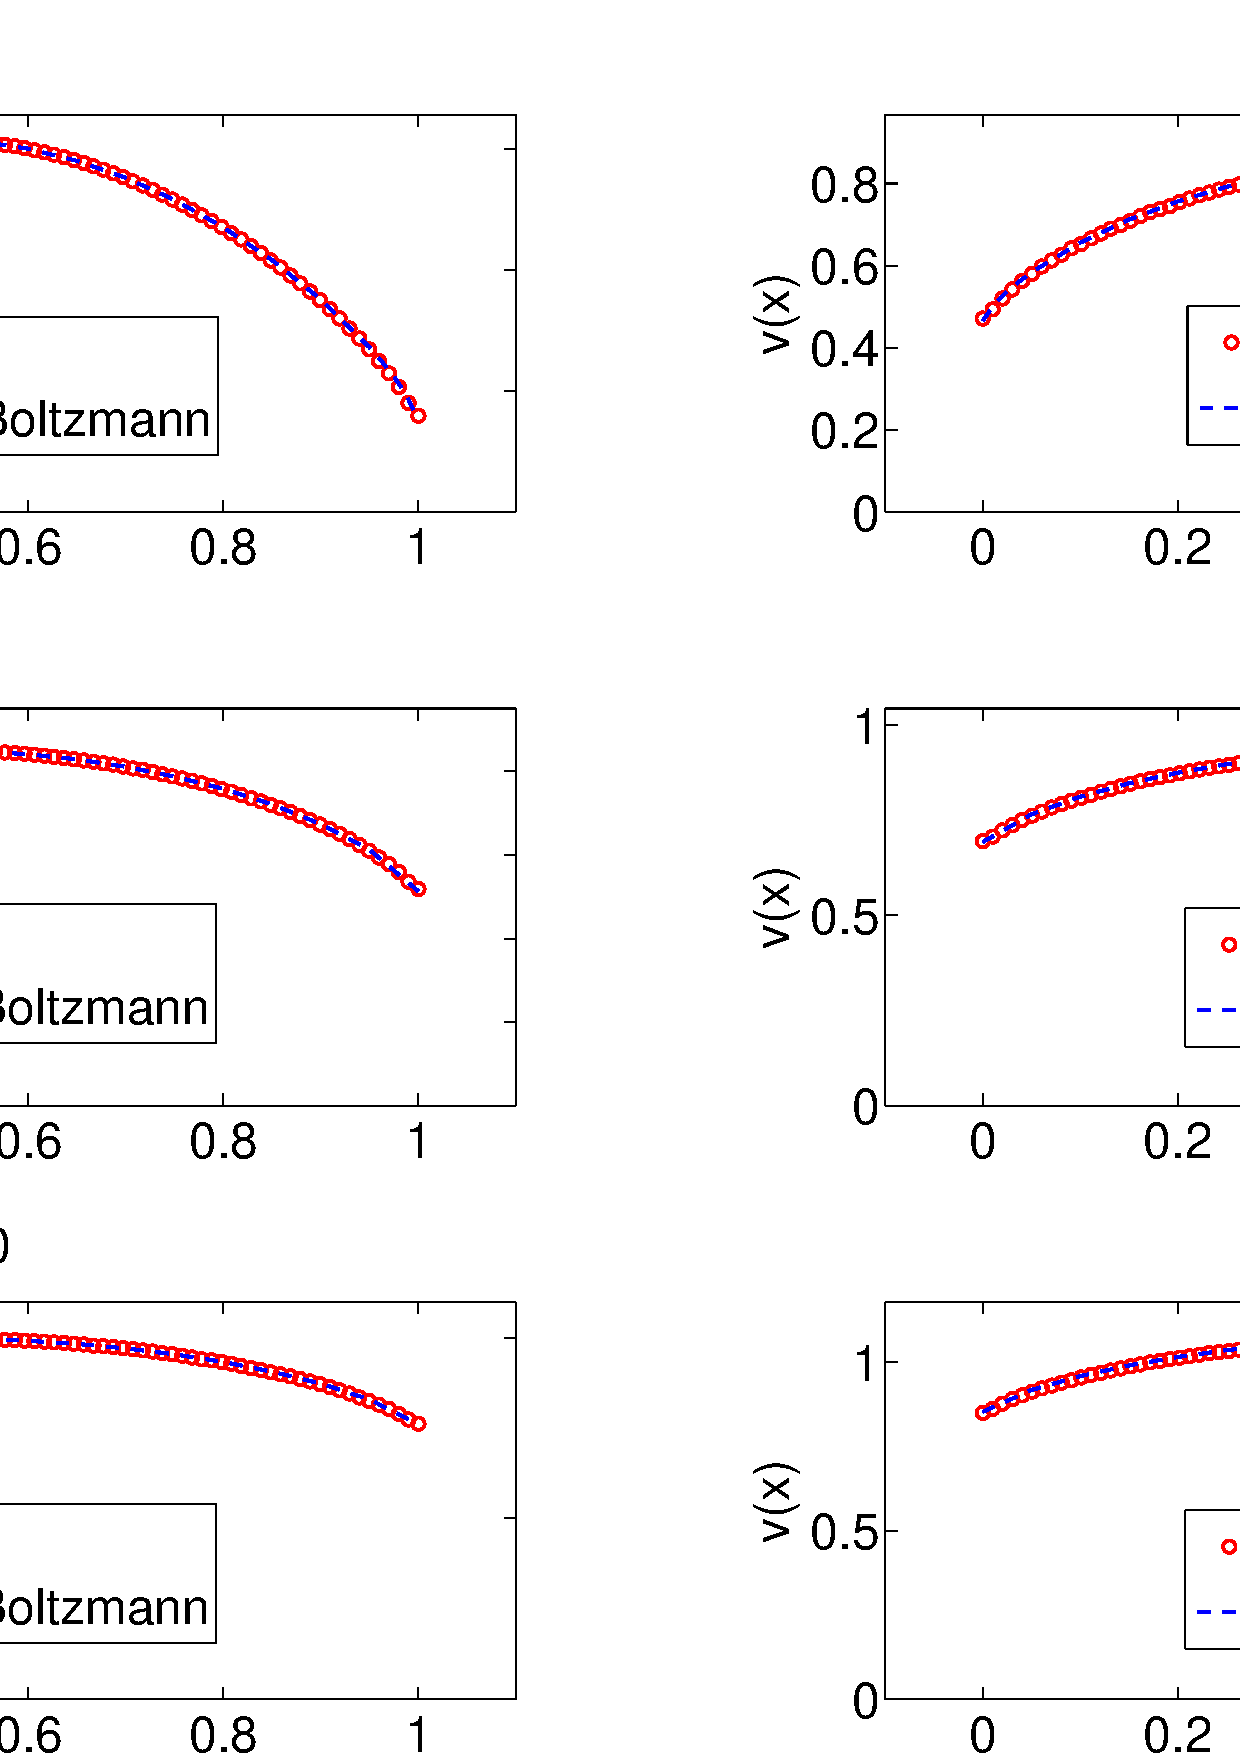
\includegraphics[scale=0.25]{figures/validation_poiseuille.pdf}
\label{fig:dsmc_validation_poiseuille}
\caption{Gravity driven Poiseuille flow}
\end{figure}

The channel is periodic in the $x-$ and $z-$direction, emulating a large system with negligible boundary effects. The gas molecules collide with the plates through the thermal wall model, so the reflected particles will have zero tangential velocity on average. In the continuum limit, $Kn\rightarrow 0$, we expect the velocity profile to approach the parabolic solution \cite{batchelor2000introduction}
\begin{align}
	v_z(y) = \nabla P\frac{1}{2\mu}y(y-h).
\end{align}
However, in the transition flow regime, $0.1 \leq Kn \leq 10$, we expect a non zero slip velocity\cite{morris1992slip}. 

The Knudsen number will affect the velocity distribution through the fact that a high Knudsen number means a larger mean free path, hence fewer inter-molecular collisions. A low collision rate will make the surface effects propagate slower through the system. We therefor expect a larger difference 

\subsubsection{Gravity driven flow}

  \section{Parallelization performance}
\label{sec:dsmc_parallelization_performance}
After the code is parallelized, the total computation time needed to perform a simulation is obviously not reduced. There are still as many collisions as before as the physical problem is identical. The idea is to do many of the calculations at the same time so that the total \textit{real} time we actually wait is reduced. Parallelizing is of course not free, as we need more logic to let the processors communicate with each other (exchanging particles and waiting for each other to finish each time step). As the number of processors increases, the total computation time \textit{per processor} is reduced, but the time spent on communication often increases. We will measure what's called \textit{parallel scalability} which indicates how efficient a program is when the number of processors is increased. There are two different kinds of scalability; weak and strong scaling
\begin{itemize}
	\item strong scaling is how the computation time changes with an increased number of processors on a fixed system size, whereas the
	\item weak scaling is how the computation time changes with an increased number of processors on a fixed system size \textit{per processor}.
\end{itemize}
\subsection{Strong scaling}
To see how the program efficiency scales with a fixed system size while increasing the number of processors is important if we want to study a specific system (a given system size and geometry, e.g. scanned from real data), but we would like to reduce the simulation run time. With a fixed system size, the total number of particles per CPU is obviously reduced while increasing the total number of processors. We define the \textit{strong scaling efficiency} $\eta_s$ as
\begin{align}
	\eta_s = \frac{t_1}{Nt_N},
\end{align}
where $t_1$ is the total run time using one processor and $t_N$ is the total run time using $N$ processors. We see that $\eta_s\in (0,1)$ since $Nt_N$ is the ideal scaling without any communication overhead. In this benchmark, we have run a geometry carved out by 10 random walkers (the algorithm is described in section \ref{sec:dsmc_random_walk_algorithm}), each starting at random positions. Each walker moves 1000 steps (voxels) with a turn probability of 0.1 on a $128\times128\times128$ voxel grid ending up with a porosity of $\phi=0.53635$. The physical system is a cube with side length $L=$\unit{1.0}{\micro\meter} with a density $\rho_n=\unit{1.0\e{25}}{\meter^{-3}}$ which gives a total of 5.3 million atoms. We choose that one DSMC particle represents one atom yielding a total of 5.3 million particles in the whole system. The benchmark was performed for 10000 timesteps ($\Delta t = 0.005$) with $2^N$ processors from 1 CPU to 512 CPUs yielding a good estimate of how efficient the program scales for a relatively large number of processors. In table \ref{tab:dsmc_strong_scaling} we have the scaling results with additional information like the number of intermolecular collisions and the number of wall collisions. These numbers indicates the amount of computation  The strong scaling efficiency is plotted against the number of processors in figure \ref{fig:dsmc_strong_scaling}.
\begin{table}
\begin{center}
    \begin{tabular}{|l|l|l|l|l|l|l}
    \hline
    $N_\text{CPU}$ & $N_\text{particles}/N_\text{CPU}$ & $N_\text{collisions}/N_\text{CPU}$ & $N_\text{wall collisions}/N_\text{CPU}$ & Run time[s] & $\eta_s$ \\ \hline
    1 & 5.4\e{6} & 1.31\e{8} & 1.09\e{11} & \unit{10571}{\second} & 1.00\\
    \hline
    2 & 2.7\e{6} & 6.55\e{7} & 5.04\e{10} &  \unit{5262}{\second} & 1.00\\
    \hline
    4 & 1.3\e{6} & 3.28\e{7} & 2.73\e{10} &  \unit{2687}{\second} & 0.984\\
    \hline
    8 & 6.7\e{5} & 1.64\e{7} & 1.36\e{10} &  \unit{1360}{\second} & 0.972\\
    \hline
    16 & 3.4\e{5} & 8.19\e{6} & 6.81\e{9} &  \unit{755}{\second} & 0.875\\
    \hline
    32 & 1.7\e{5} & 4.09\e{6} & 3.41\e{9} &  \unit{505}{\second} & 0.654\\
    \hline
    64 & 8.4\e{4} & 2.05\e{6} & 1.70\e{9} &  \unit{262}{\second} & 0.630\\
    \hline
    128 & 4.2\e{4} & 1.02\e{6} & 8.52\e{8} &  \unit{146}{\second} & 0.566\\
    \hline
    256 & 2.1\e{4} & 5.12\e{5} & 4.26\e{8} &  \unit{94}{\second} & 0.440\\
    \hline
    512 & 1.0\e{4} & 2.56\e{5} & 2.13\e{8} &  \unit{79}{\second} & 0.261\\
    \hline
    \end{tabular}
    \caption{Benchmark results showing the strong scaling efficiency $\eta_s$ for the DSMC program.}
    \label{tab:dsmc_strong_scaling}
    \end{center}
\end{table}
The reason for this scaling behavior might be due to bad load balancing since the processors might get different work load. One processor might get a subvolume that contains very few particles if most of its voxels are solid wall voxels. These processors will spend most of their time on waiting for the other processors to finish and we do not make full use of the available processors. This problem is discussed further in section \ref{sec:future_work_load_balancing}. 
\subsection{Weak scaling}
Another important scaling problem appears when we want to maximize the simulated system size. If we keep a constant system size \textit{per cpu}, and increase the number of processors, the limitation of how big we efficiently can create the system is controlled by the weak scaling. We then introduce the \textit{weak scaling efficiency} $\eta_w$ defined as
\begin{align}
	\eta_w = \frac{t_1}{t_N},
\end{align}
where again $t_1$ is the total run time using one processor and $t_N$ is the run time using $N$ processors. If the algorithm scales perfectly, the total run time would remain constant while increasing the number of processors (each CPU is ideally independent), but we expect some overhead. This implies that the range for $\eta_w$ also is between zero and one. We have run the same geometry as for the strong scaling, but each processor controls a volume of \unit{1}{\micro\meter^3} so that the largest system is \unit{512}{\micro\meter^3}. Keeping the same density gives a total of 5.3 million particles per processor. In table \ref{tab:dsmc_weak_scaling}, we see the results for the weak scaling efficiency simulation. 
\begin{table}
\begin{center}
    \begin{tabular}{|l|l|l|l|l|l|l}
    \hline
    $N_\text{CPU}$ & $N_\text{particles}$ & $N_\text{collisions}$ & $N_\text{wall collisions}$ & Run time[s] & $\eta_w$ \\ 
    \hline
    1 & 5.4\e{6} & 1.00\e{10} & 1.00\e{10} & \unit{100}{\second} & 1.0\\
    \hline
    2 & 1.27\e{6} & 1.00\e{10} & 1.00\e{10} & \unit{100}{\second} & 1.0\\
    \hline
    4 & 1.27\e{6} & 1.00\e{10} & 1.00\e{10} & \unit{100}{\second} & 1.0\\
    \hline
    8 & 1.27\e{6} & 1.00\e{10} & 1.00\e{10} & \unit{100}{\second} & 1.0\\
    \hline
    16 & 1.27\e{6} & 1.00\e{10} & 1.00\e{10} & \unit{100}{\second} & 1.0\\
    \hline
    32 & 1.27\e{6} & 1.00\e{10} & 1.00\e{10} & \unit{100}{\second} & 1.0\\
    \hline
    64 & 1.27\e{6} & 1.00\e{10} & 1.00\e{10} & \unit{100}{\second} & 1.0\\
    \hline
    128 & 6.87\e{8} & 1.67\e{10} & 5.86\e{11} & \unit{12032}{\second} & 1.0\\
    \hline
    256 & 1.37\e{9} & 3.33\e{10} & 1.05\e{12} & \unit{16418}{\second} & 1.0\\
    \hline
    512 & 2.75\e{9} & 6.59\e{10} & 1.87\e{12} & \unit{18242}{\second} & 1.0\\
    \hline
    \end{tabular}
    \caption{Benchmark results showing the weak scaling efficiency $\eta_w$ for the DSMC program.}
    \label{tab:dsmc_weak_scaling}
    \end{center}
\end{table}

\begin{figure}[h]
\begin{center}
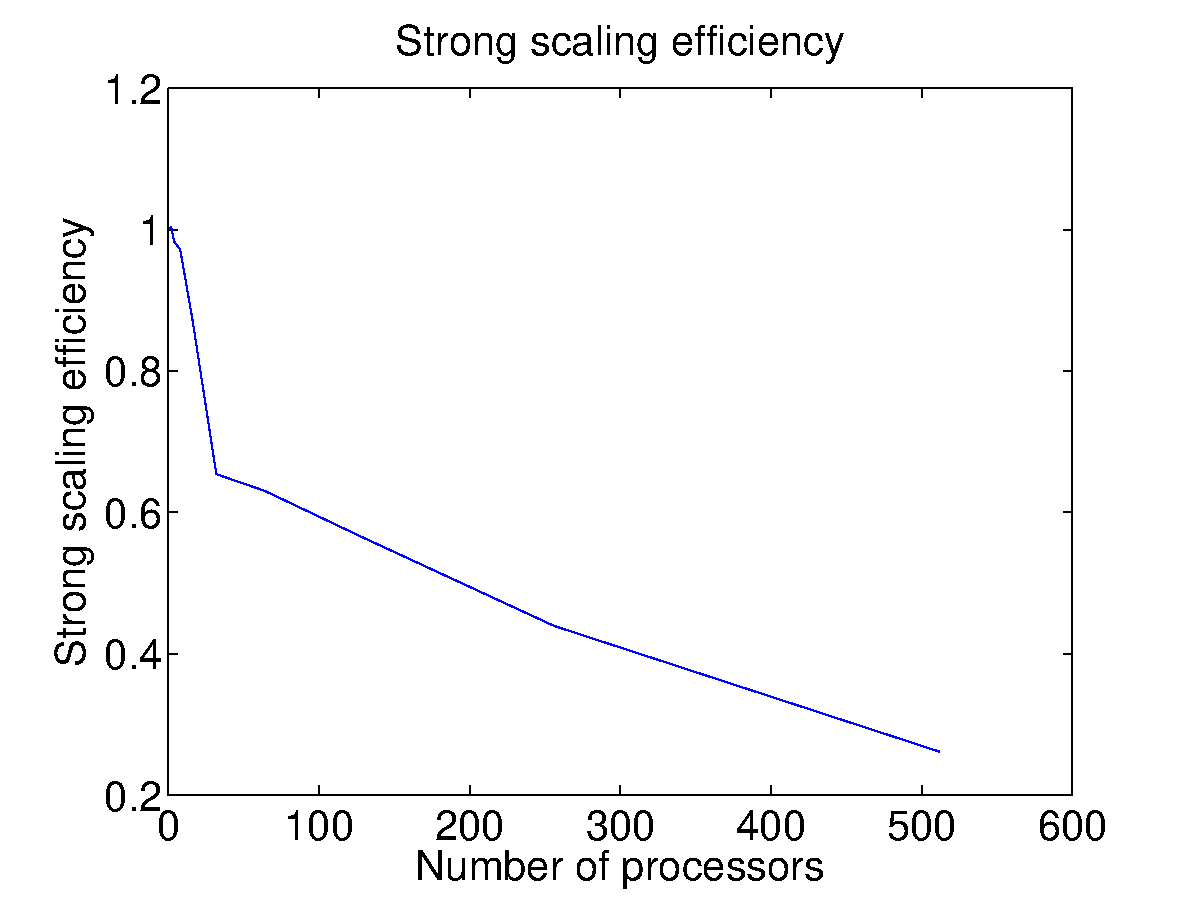
\includegraphics[width=\textwidth, trim=0cm 0cm 0cm 0cm, clip]{DSMC/figures/strong_scaling.eps}
\end{center}
\caption{The weak and strong scaling efficiency, $\eta_w$ and $\eta_s$, as a funtion of the number of processors $N_\text{CPU}$. We see that at 512 processors, the efficiency is reduced to 25\% because of the large overhead from the MPI communication.}
\label{fig:dsmc_strong_scaling}
\end{figure}
\section{Results for simple geometries}
\label{sec:results_for_simple_geometries}
In this section, we will study flow in simple geometries where the theoretical permeability is well known. The expression for the permeability is only valid for small Knudsen numbers (which we called the absolute permeability; the permeability for fluids in the continuum limit), so it is a perfect test case for the Knudsen correction factor $f_c$ in equation \eqref{eq:knudsen_correction}. 

\subsection{Flow in a cylinder, varying Knudsen number}
We have induced flow in a cylinder with radius \unit{0.45}{\micro\meter} with an applied acceleration corresponding to a pressure difference $\Delta P = 1.1P_0$, where $P_0$ is the ideal gas pressure at \unit{300}{\kelvin}. We want to vary the Knudsen number which was defined as
\begin{align}
	\text{Kn} = \frac{\lambda}{L} = \frac{1}{\sqrt 2 \pi d^2 \rho_n L}
\end{align}
where $L$ is the length of the cylinder, $\lambda$ is the mean free path. We have used equation \eqref{eq:mean_free_path} in the last expression so that we can choose the Knudsen number through the density
\begin{align}
	\rho_n(\text{Kn}) = \frac{1}{\sqrt 2 \pi d^2 \text{Kn}L}.
\end{align}
We expect an apparent permeability satisfying the Knudsen correction
\begin{align}
	k_a = k_\infty f_c = k_\infty[1 + \alpha(\text{Kn})\text{Kn}]\left[1 + {4\text{Kn}\over 1 + \text{Kn}}\right].
\end{align}
The analytical absolute permeability for a cylinder with radius $r$ is given by\cite{karniadakis2005microflows}
\begin{align}
	\label{eq:permeability_cylinder}
	k_\infty = {r^2\over 8},
\end{align}
which gives the following prediction for the apparent permeability
\begin{align}
	k_a = [1 + \alpha(\text{Kn})\text{Kn}]\left[1 + {4\text{Kn}\over 1 + \text{Kn}}\right] {r^2\over 8}.
\end{align}
In figure \ref{fig:one_cylinder_varying_knudsen} we have plotted the measured permeability as a function of Knudsen number. We see that the 

\begin{figure}[h]
\begin{center}
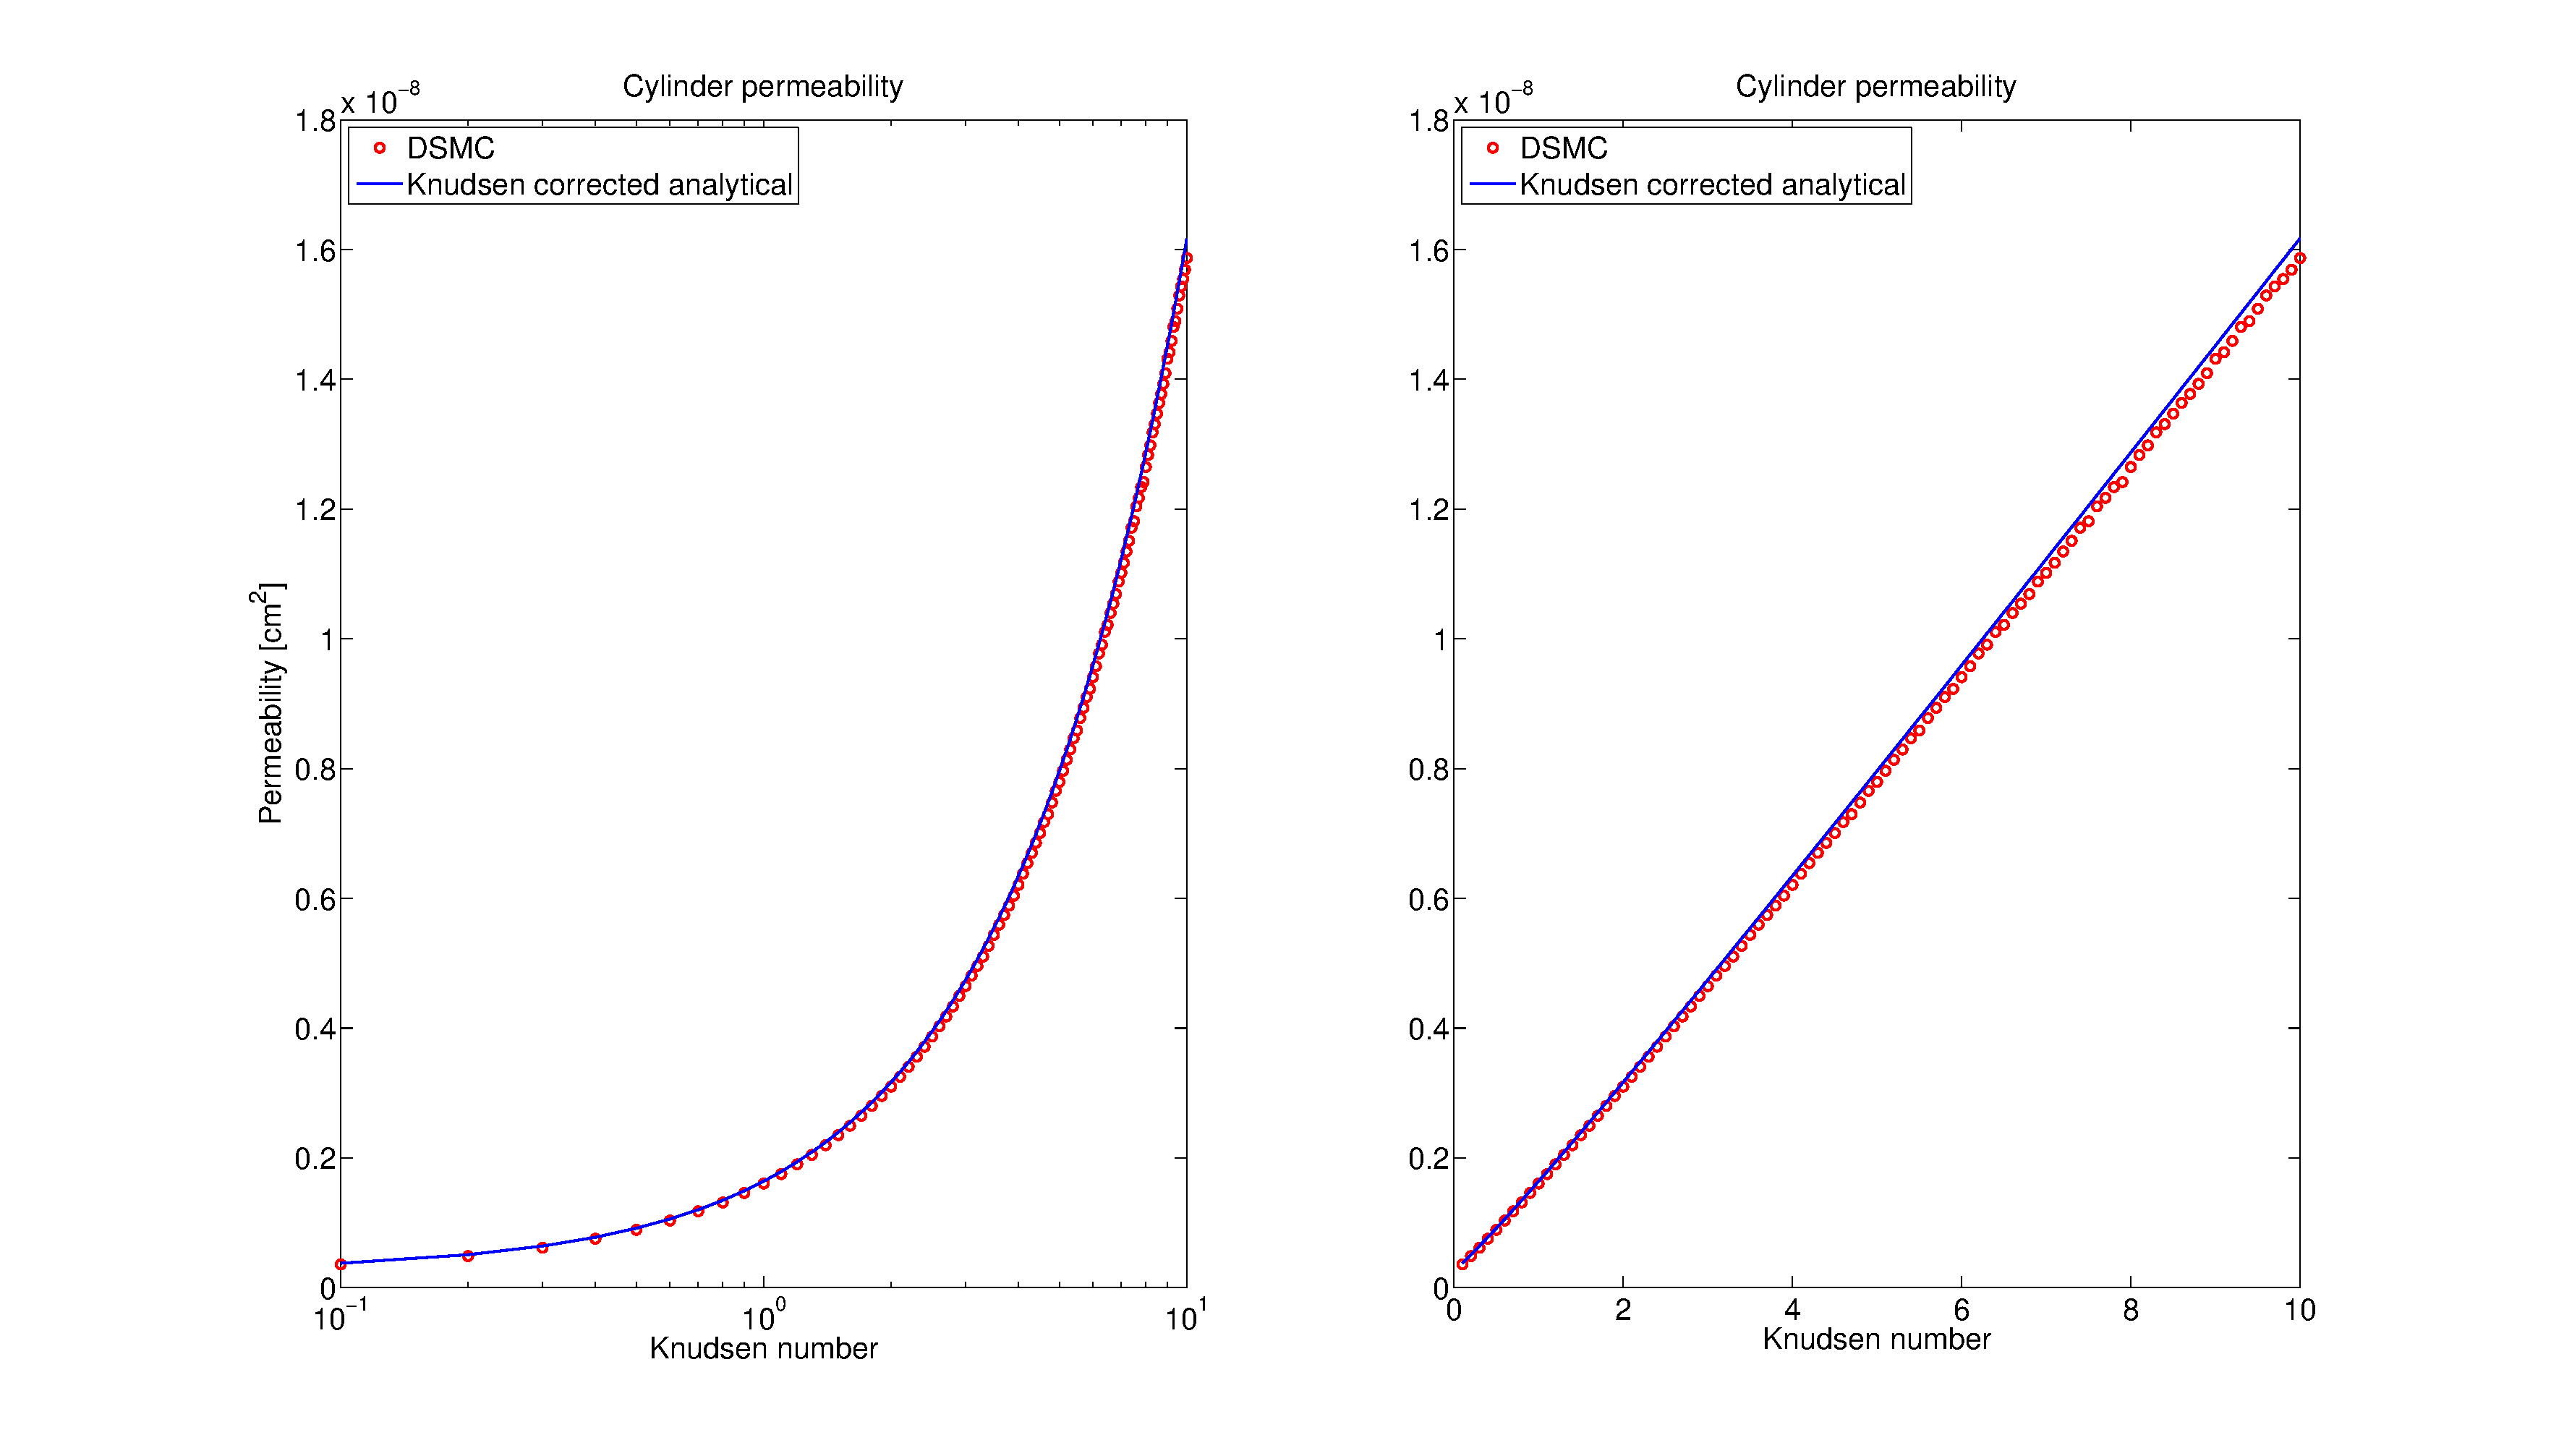
\includegraphics[width=\textwidth, trim=0cm 0cm 0cm 0cm, clip]{DSMC/figures/cylinder_knudsen_permeability.eps}
\end{center}
\caption{Permeability as a function of Knudsen number for a cylinder with radius \unit{0.45}{\micro\meter} and length \unit{1}{\micro\meter} with an applied pressure difference $\Delta P = 1.1P_0$ ($P_0$ being the ideal gas pressure). We control the Knudsen number by varying the density. The blue line is the Knudsen corrected analytical solution from \cite{karniadakis2005microflows}. The DSMC results confirm that the Knudsen correction factor works very well for a system with a well defined Knudsen number.}
\label{fig:one_cylinder_varying_knudsen}
\end{figure}

\subsection{Flow in a cylinder, varying radius}
If we instead keep the Knudsen number constant ($\text{Kn}=1.0$), we can vary the radius to verify equation \eqref{eq:permeability_cylinder}. We have studied radii in the range \unit{0.1}{\micro\meter} to \unit{0.45}{\micro\meter} with the same pressure difference as in the previous simulation ($\Delta P = 1.1P_0)$. In figure \ref{fig:one_cylinder_varying_radii_result} we have plotted the measured permeability as a function of cylinder radius. The straight line confirms the quadratic dependency in equation \eqref{eq:permeability_cylinder}.
\begin{figure}[h]
\begin{center}
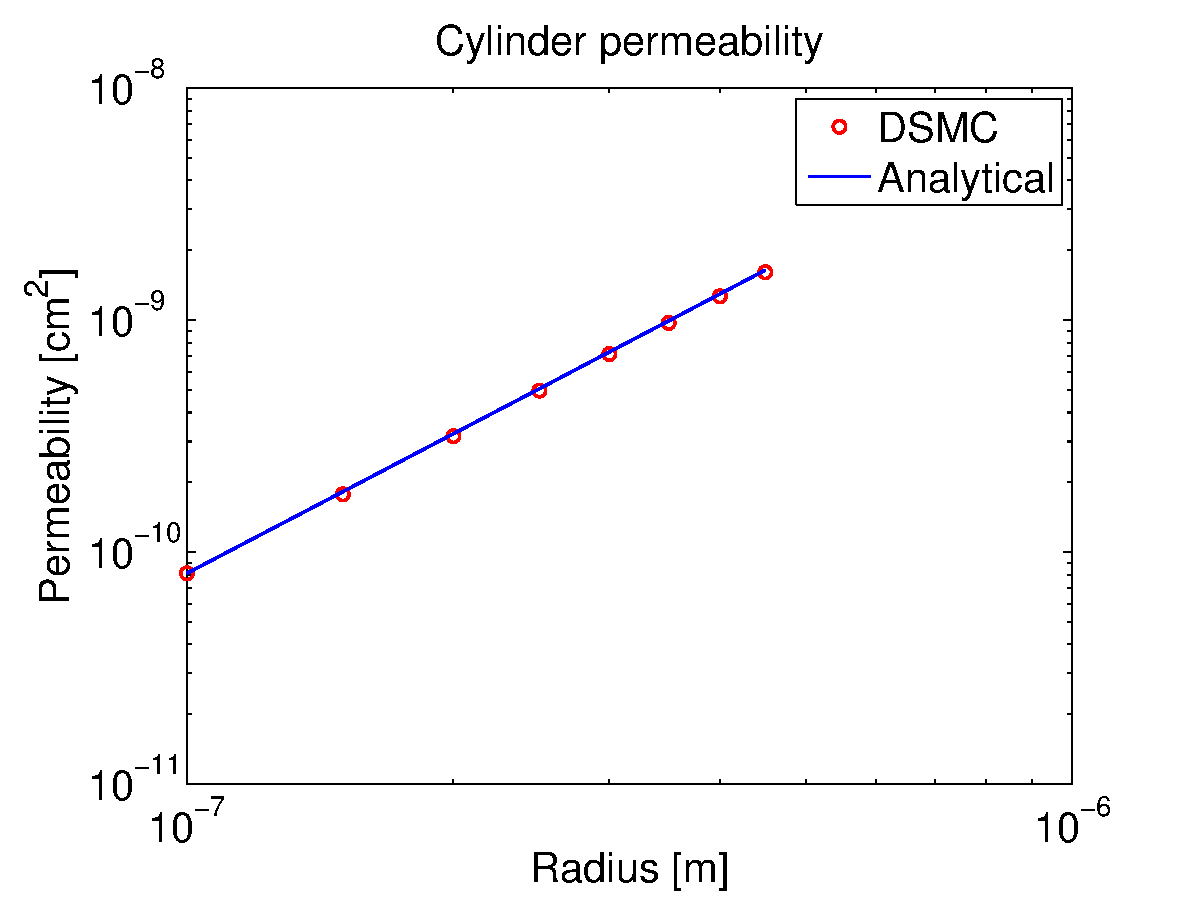
\includegraphics[width=\textwidth, trim=0cm 0cm 0cm 0cm, clip]{DSMC/figures/cylinder_radius_permeability.eps}
\end{center}
\caption{Logarithmic plot of the permeability for different cylinders with radii in the range $0.1 \mu m$ to $0.45 \mu m$ with an applied pressure difference $\Delta P = 1.1P_0$. The blue line is the Knudsen corrected analytical solution from \cite{karniadakis2005microflows}.}
\label{fig:one_cylinder_varying_radii_result}
\end{figure}
\section{Results for complicated geometries}
We have now seen that the Knudsen correction factor works well for systems with a well defined Knudsen number. The Knudsen correction factor needs an exact Knudsen number to be able to predict the permeability, but for more complex geometries, there is rather a distribution of Knudsen numbers than a single number. It could work as a lower and an upper limit of the permeabilities for two different input Knudsen numbers, but they could differ by an order of magnitude. In this section we will study a system consisting of randomly packed spheres that does not have a well defined Knudsen number.
\subsection{The Carman-Kozeny equation}
In 1927, Kozensky proposed an equation predicting the permeability of packed spheres of radius $a$ forming a system with porosity $\phi$ given as
\begin{align}
	k = {a^2 \over 9K} {\phi^3 \over (1 - \phi)^2},
\end{align}
where $K$ is the Kozeny constant which is experimentally measured to be around five\cite{carman1937fluid}. This result has been verified to predict permeabilities in many experiments since its discovery. However, at the nanometer scale, we expect deviations due to high Knudsen numbers. 
\subsection{The simulation}

\end{chapter}
\end{part}

\begin{part}{Molecular Dynamics}
  \label{part:md}
  \begin{chapter}{Theory}
  \label{chap:md}
  Molecular Dynamics is another numerical model that describes the behaviour of liquids, gases and solids at the finest scale of any classical model. We can study the dynamics of single atoms and how they interact with each other forming molecules and larger objects like advanced pore networks. The idea is simple and has been used since the time of Sir Isaac Newton in the 17th century when he formulated his laws of motion. With the knowledge of the relevant forces between the atoms, we can solve Newton's equations and calculate their dynamics.

We open this chapter by a short introduction to the model in section \ref{sec:md_model} before we explain how forces are calculated with the Lennard-Jones potential in section \ref{sec:md_forces}. With computed forces, we can integrate the atoms with Newton's laws following an time integration scheme which we discuss in section \ref{sec:md_time_integration}. The last section is concerned with how we measure physical quantities which will be very similar to what we did with DSMC in section \ref{sec:dsmc_measuring_physical_quantities}.
  \section{The model}
\label{sec:md_model}
The state of a Molecular Dynamics system is fully described by seven variables per atom; three positions, three velocities plus the atom type. The phase variables are evolved through the laws of motion. It is here common, as in DSMC (see section \ref{sec:dsmc_model}), to apply periodic boundary conditions. Applied periodic boundary conditions in all directions implies constant volume (unless, of course, we rescale the system size which can be done). The atomic forces are calculated as the gradient of a chosen potential that can differ quite a lot depending on the requirements of the model. A noble gas like Argon can be modeled with a simple potential called the Lennard-Jones potential which will be discussed below. With this potential, one can calculate equilibrium thermodynamic properties that are in good agreement with experimental values \cite{verlet1967computer}. System statistics are sampled as ensemble averages through ergodicity over large times. A typical Molecular Dynamics algorithm is illustrated in figure \ref{fig:flow_simple_md}.
\begin{figure}[h]
\framebox{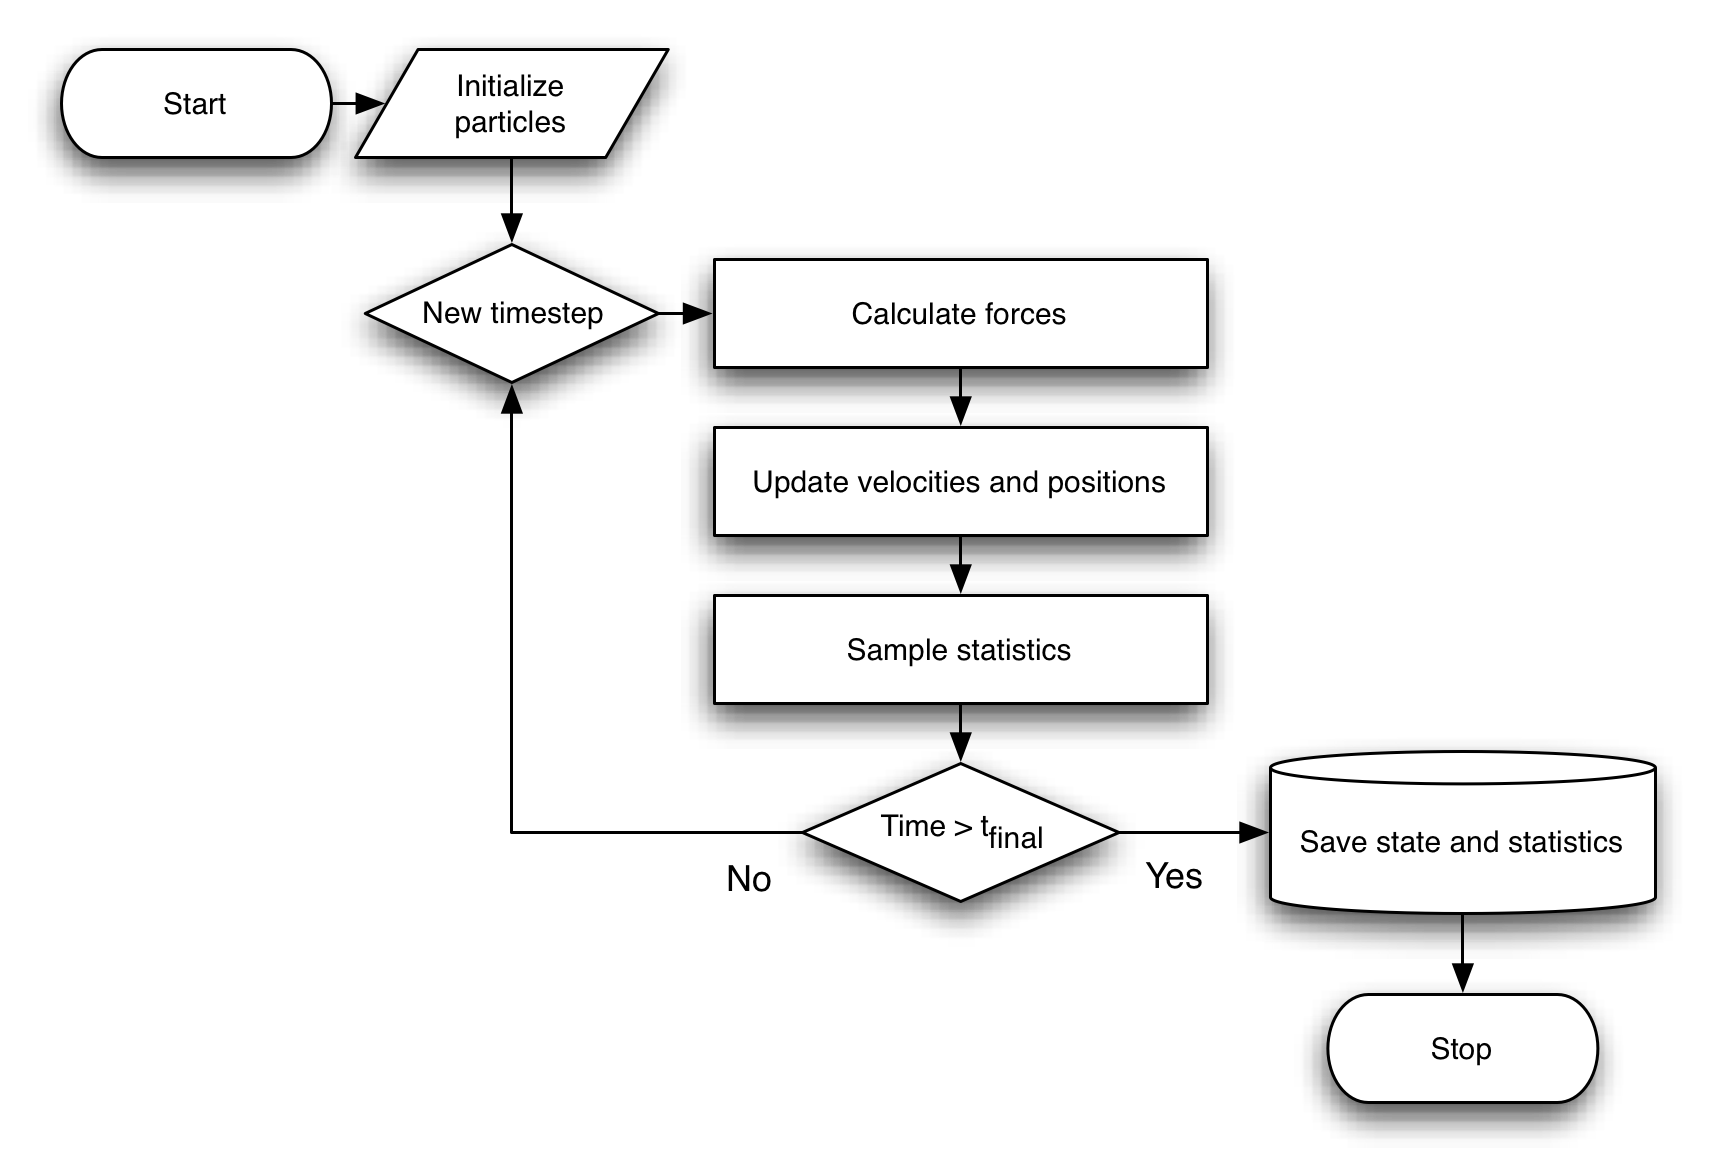
\includegraphics[width=0.8\textwidth, trim=0cm 0cm 0cm 0cm, clip]{MD/figures/SimpleMD.png}}
\centering
\caption{Flow chart illustrating a typical Molecular Dynamics algorithm.}
\label{fig:flow_simple_md}
\end{figure}
  \section{Force calculation - potentials}
\label{sec:md_forces}
In general, the potential energy is given as a function of the configuration given by the atom positions
\begin{align}
	U(\vec{r}) = \sum_{i<j}U_2(r_{ij}) + \sum_{i<j<k} U_r(\vec r_i, \vec r_j, \vec r_k) + ...,
\end{align}
where $\vec r$ is the phase space point, $U_n$ is a function of the positions of $n$ atoms, $r_{ij}$ is the relative distance between atom $i$ and $j$, $\vec r_i$ is the position of atom $i$. Advanced potentials such as ReaxFF can even have 5-atom contributions to the energy\cite{van2001reaxff}. The reason for this is simple; when three atoms are close to each other, the electron configuration might be different than if there were only two atoms. These effects play a large role in forming molecules, such as water. Numerically, the calculation of forces is the most expensive part of the whole program, so for simple systems or educationally purposes it might be sufficient to use the Lennard-Jones potential.
\subsection{The Lennard-Jones potential}
We often see this potential referred to as the 6-12 potential, due to its functional form. It is a function that inherently carries the two main properties of atomic forces; the short-ranged Pauli repulsion and the long-ranged van der Waals force. The potential is only between pairs of atoms
\begin{align}
	\label{eq:md_potential_energy}
	U_{LJ}(r_{ij}) = 4\epsilon\left[\left(\frac{\sigma}{r_{ij}}\right)^{12} - \left(\frac{\sigma}{r_{ij}}\right)^{6}\right],
\end{align}
where $r_{ij}$ is the relative distance between atom $i$ and $j$, $\epsilon$ and $\sigma$ are coupling constants giving the depth of the potential well and the distance where the potential is zero. The force is given as the gradient of this potential yielding 
\begin{align}
	\label{eq:md_lj_force}
	\vec F_{LJ}(\vec{r_{ij}}) = -\nabla U_{LJ}(r_{ij}) = -24\epsilon\left[2\left(\frac{\sigma^{12}}{r_{ij}^{13}}\right) - \left(\frac{\sigma^6}{r_{ij}^7}\right)\right]\vec u_{ij},
\end{align}
where $\vec u_{ij}$ is the unit vector pointing from atom $i$ to atom $j$. In this thesis, we will only study the LJ-potential, so we simplify the notation by choosing $\vec F_{LJ} = \vec F$ and $U_{LJ} = U$. The form of the potential is shown in figure \ref{fig:md_lennard_jones}.
\begin{figure}[h]
\begin{center}
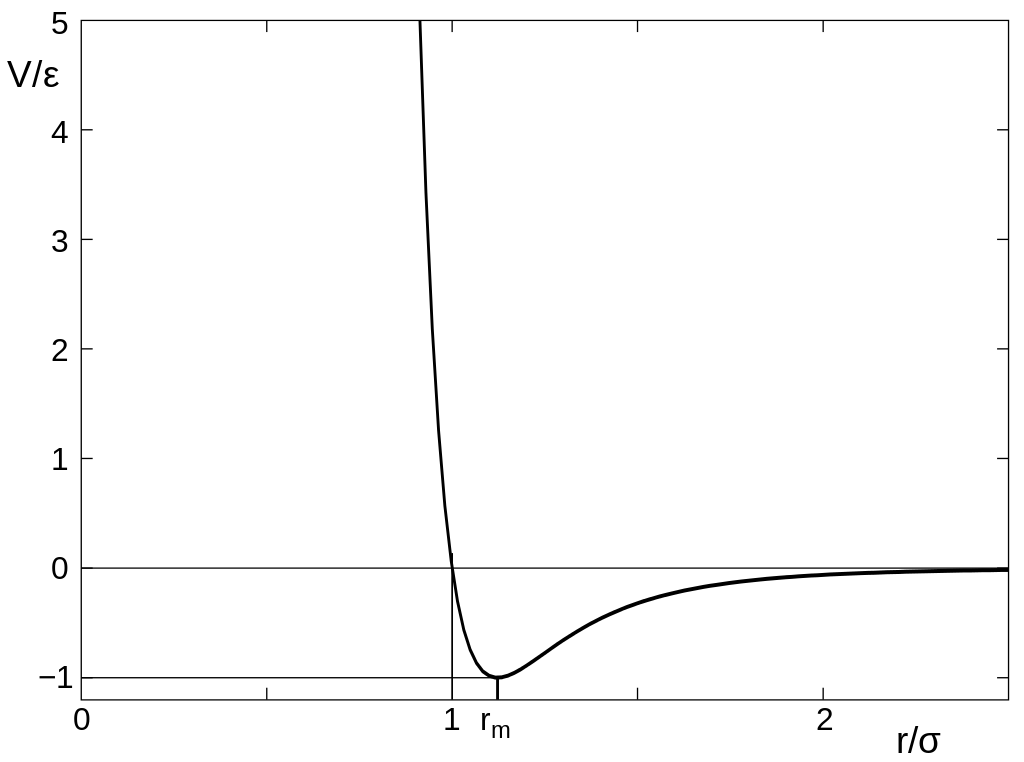
\includegraphics[width=0.8\textwidth, trim=0cm 0cm 0cm 0cm, clip]{MD/figures/lennard_jones.png}
\end{center}
\caption{The Lennard-Jones potential as a function of relative distance $r_{ij}$ between two atoms. (Image from \url{http://en.wikipedia.org/wiki/File:12-6-Lennard-Jones-Potential.svg}, accessed 18 March, 2014.)}
\label{fig:md_lennard_jones}
\end{figure}
With this potential, we can in principle calculate the forces between atoms that are 10 meters apart. We already know the answer though, it should be very, very close to zero. Atoms being far away from each other do not interact. This distance is actually not very large. If we insert $r_{ij} = 3.0\sigma$ into equation \eqref{eq:md_lj_force}, and choose units so that $\sigma = \epsilon = 1.0$, we get $F(r=3.0) \approx 0.01$ (compared to the maximum attraction near the potential well $F(r = 1.24) \approx 2.4$, more than 100 times larger). The force decreases slowly towards zero for larger displacements. We can exploit this property and only compute forces between atoms displaced by a distance smaller than some cut-off radius.
\subsection{Cut-off radius}
\label{sec:md_implementation_two_body_forces}
In principle, we have to sum over all pairs in the system which for $N$ atoms is $O(N^2)$. This calculation can be reduced to $O(N)$ by realizing that the gradient of the potential (hence the force) is nearly zero at $r \approx 2.5\sigma$. We now introduce the cut-off radius $r_\text{cut}$, which we choose to be $r_\text{cut} = 2.5\sigma$. The force between a pair of atoms $F(r_{ij})$ is then written as
\begin{align}
	\vec F(\vec r_{ij}) = \left\{
	\begin{array}{l l}
		-24\epsilon\left[2\left(\frac{\sigma^{12}}{r_{ij}^{13}}\right) - \left(\frac{\sigma^6}{r_{ij}^7}\right)\right]\vec u_{ij} & \text{if } r_{ij} \leq r_\text{cut}\\
		0 & \text{if } r_{ij} > r_\text{cut}.
	\end{array}\right .
\end{align}
This means that we don't have to compute the forces between atoms that are more than $r_\text{cut}$ apart. So \textit{locally}, within this radius $r_\text{cut}$, the number of pairs we need to sum over is proportional to $\rho_n^2$, but if we double the system size, most of the extra atoms do not feel the forces from the atoms already in the system since they are separated by more than $r_\text{cut}$. So the calculation of forces is $O(N)$.
  \section{Pressure driven flows}
We will induce flow in the same way we did in section \ref{sec:dsmc_pressure_driven_flows}. We apply a 
  \section{Time integration}
\label{sec:md_time_integration}
The idea of doing a Molecular Dynamics simulation is to start from some initial state $(\vec r_0, \vec v_0)$ and compute the time evolution of atoms following Newton's equations with the defined forces. We will use this time evolution to sample statistics from states in the phase space, assuming that the time evolution will guide the system through the phase space with probabilities according to the statistical ensemble. This was the assumtion of ergodicity. In a standard Molecular Dynamics simulation, we want to sample states from the microcanonical ensemble (NVE) where the energy, volume and number of atoms are conserved. Our choice of time integrator should therefore conserve energy as good as possible. A good choice is the Velocity Verlet algorithm, which is known to be both fast and conserve energy quite well\cite{frenkel2001understanding}.\\
The Velocity Verlet algorithm requires the knowledge of the positions, velocities and instantaneous accelerations of the atoms. The latter is found through the force on an atom $\vec a_i = \vec F_i/m_i$, so it requires the storage of $9N$ variables in a system with $N$ atoms. We have derived the Velocity Verlet algorithm using the Liouville formulation of time evolution in appendix \ref{app:liouville}. The integration steps are
\begin{align}
	\vec v(t + \Delta t/2) &= \vec v(t) + \frac{\vec F(t)}{m}\frac{\Delta t}{2}\\
	\vec r(t + \Delta t) &= \vec r(t) + \vec v(t + \Delta t/2)\Delta t\\
	\vec v(t + \Delta t) &= \vec v(t + \Delta t/2) + \frac{\vec F(t + \Delta t)}{m}\frac{\Delta t}{2},
\end{align}
which is done each timestep for every atom in the system. We call the first step a \textit{half kick}, because it integrates the velocity with forward Euler with half a timestep. The position is then also integrated with forward Euler with the full timestep $\Delta t$ before we do another half kick.
  \section{Physical properties}
The phase space variables can be used to sample statistical properties of the system. Properties of interest are kinetic and potential energy, temperature, pressure, diffusion constant and different correlation functions (such as the pair correlation function, cage-correlation function, static and the dynamic structure factor). In this section, we will define these properties and discuss how to measure them.
\subsection{Kinetic and potential energy}
We measure the kinetic energy directly through its definition for point particles
\begin{align}
	E_k = \sum_i \frac{1}{2} m_iv_i^2,
\end{align}
where $m_i$ is the mass of particle $i$ and $v_i$ is the velocity of the particle. The potential energy is measured by evaluating \eqref{eq:md_potential_energy}. We define temperature by applying the equipartition theorem using the momentum degrees of freedom
\begin{align*}
	E_k = \frac{f}{2}kT,
\end{align*}
where $f=3N$ are the three momentum variables per particle, $T$ is the temperature and $k$ is Boltzmann's constant. Solving the equation for the temperature yields
\begin{align}
	T = \frac{2E_k}{3Nk},
\end{align}
which is how we \textit{define} temperature in this model. 
\subsection{Pressure}
We will derive an expression for the pressure by using Clausius' virial function
\begin{align}
    W(\textbf{r}) = \sum_{i=1}^N \vec r_i \cdot \vec F_i^{TOT},
\end{align}
where $F_i^{TOT}$ is the total force acting on atom $i$, including external forces. We assume equilibrium, so that the kinetic energy has reached an approximately constant value. We measure the statistical average of $W$ by calculating
\begin{align}
    \langle W \rangle &= \lim_{t\rightarrow\infty} {1\over t} \int_0^t d\tau \sum_{i=1}^N \vec r_i(\tau) \cdot m_i \vec{\ddot r}_i(\tau).
\end{align}
Integrating by parts gives
\begin{align}
    \label{eq:virial_and_equi}
    \langle W \rangle &= -\lim_{t\rightarrow\infty} {1\over t} \int_0^t d\tau \sum_{i=1}^N m_i |\vec{\dot r}_i(\tau)|^2 = -2E_k = -3Nk_bT,
\end{align}
by again using equipartition. Now, assume that the atoms live inside a parallelepipedic container of size $L_x, L_y, Lz$ with hard walls, with origo in one of its corners. If we divide the force into external and interatomic forces, $\vec F_i^{TOT} = \vec F_i + \vec F_i^{EXT}$, and assume that the external forces are forces from the container (no gravity or electric fields), we can calculate $W^{EXT}$. The atoms near the walls apply a pressure on the wall $P = F/A$. As an example, we look at all the atoms that are near the wall located at $x=L_x$. The virial function gives
\begin{align}
    W^{EXT}_x = \sum_{n=1}^{N_x}\vec r_n\cdot \vec F_n^{EXT},
\end{align}
where $n$ now sums over all atoms that are near the container wall at $x=L_x$. The position vectors are $\vec r_n = (L_x, y_n, z_n)$ and the force only has a component normal to the wall $F_n^{EXT} = 1/N_x(-PL_yL_z, 0, 0)$. We then get
\begin{align}
    W^{EXT}_x = -L_xPL_yL_z = -PV,
\end{align}
and by doing the same for the other dimensions, we get
\begin{align}
    W = -3PV.
\end{align}
Inserting this result into \eqref{eq:virial_and_equi} yields
\begin{align}
    \left\langle \sum_{i=1}^N \vec r_i \cdot \vec F_i\right\rangle - 3PV = -3Nk_bT
\end{align}
which can be rearranged to
\begin{align}
    PV = Nk_bT - \frac{1}{3}\left\langle \sum_{i=1}^N \vec r_i \cdot \vec F_i\right\rangle.
\end{align}
Using this result, we can define the pressure
\begin{align}
	P = \rho k_bT - \frac{1}{3V}\left\langle \sum_{i=1}^N \vec r_i \cdot \vec F_i\right\rangle,
\end{align}
where $\rho$ is the density.
\subsection{Radial distribution function $g(r)$}
The thermodynamic properties like temperature, pressure and volume give little or no information about the microscopic structure of the system. If the atoms forms a solid and are organized in some sort of a crystal (see figure \ref{fig:crystal}), one could be interested in measuring what kind of crystal they form. Different structures and symmetries of the crystal give rise to different physical properties like electronic band structure, optical transparency among others\cite{kittel1996introduction}. The crystal structure can be studied through what is called the radial distribution function, $g(r)$, which is a function proportional to the probability of finding an atom at a distance $r$ from another atom. A non-perfect FCC lattice (non-perfect in the sense that the atoms are vibrating around the equilibrium) will have a $g(r)$ as in figure \ref{fig:fcc_lattice_g_of_r}.\\
\begin{figure}[h]
\framebox{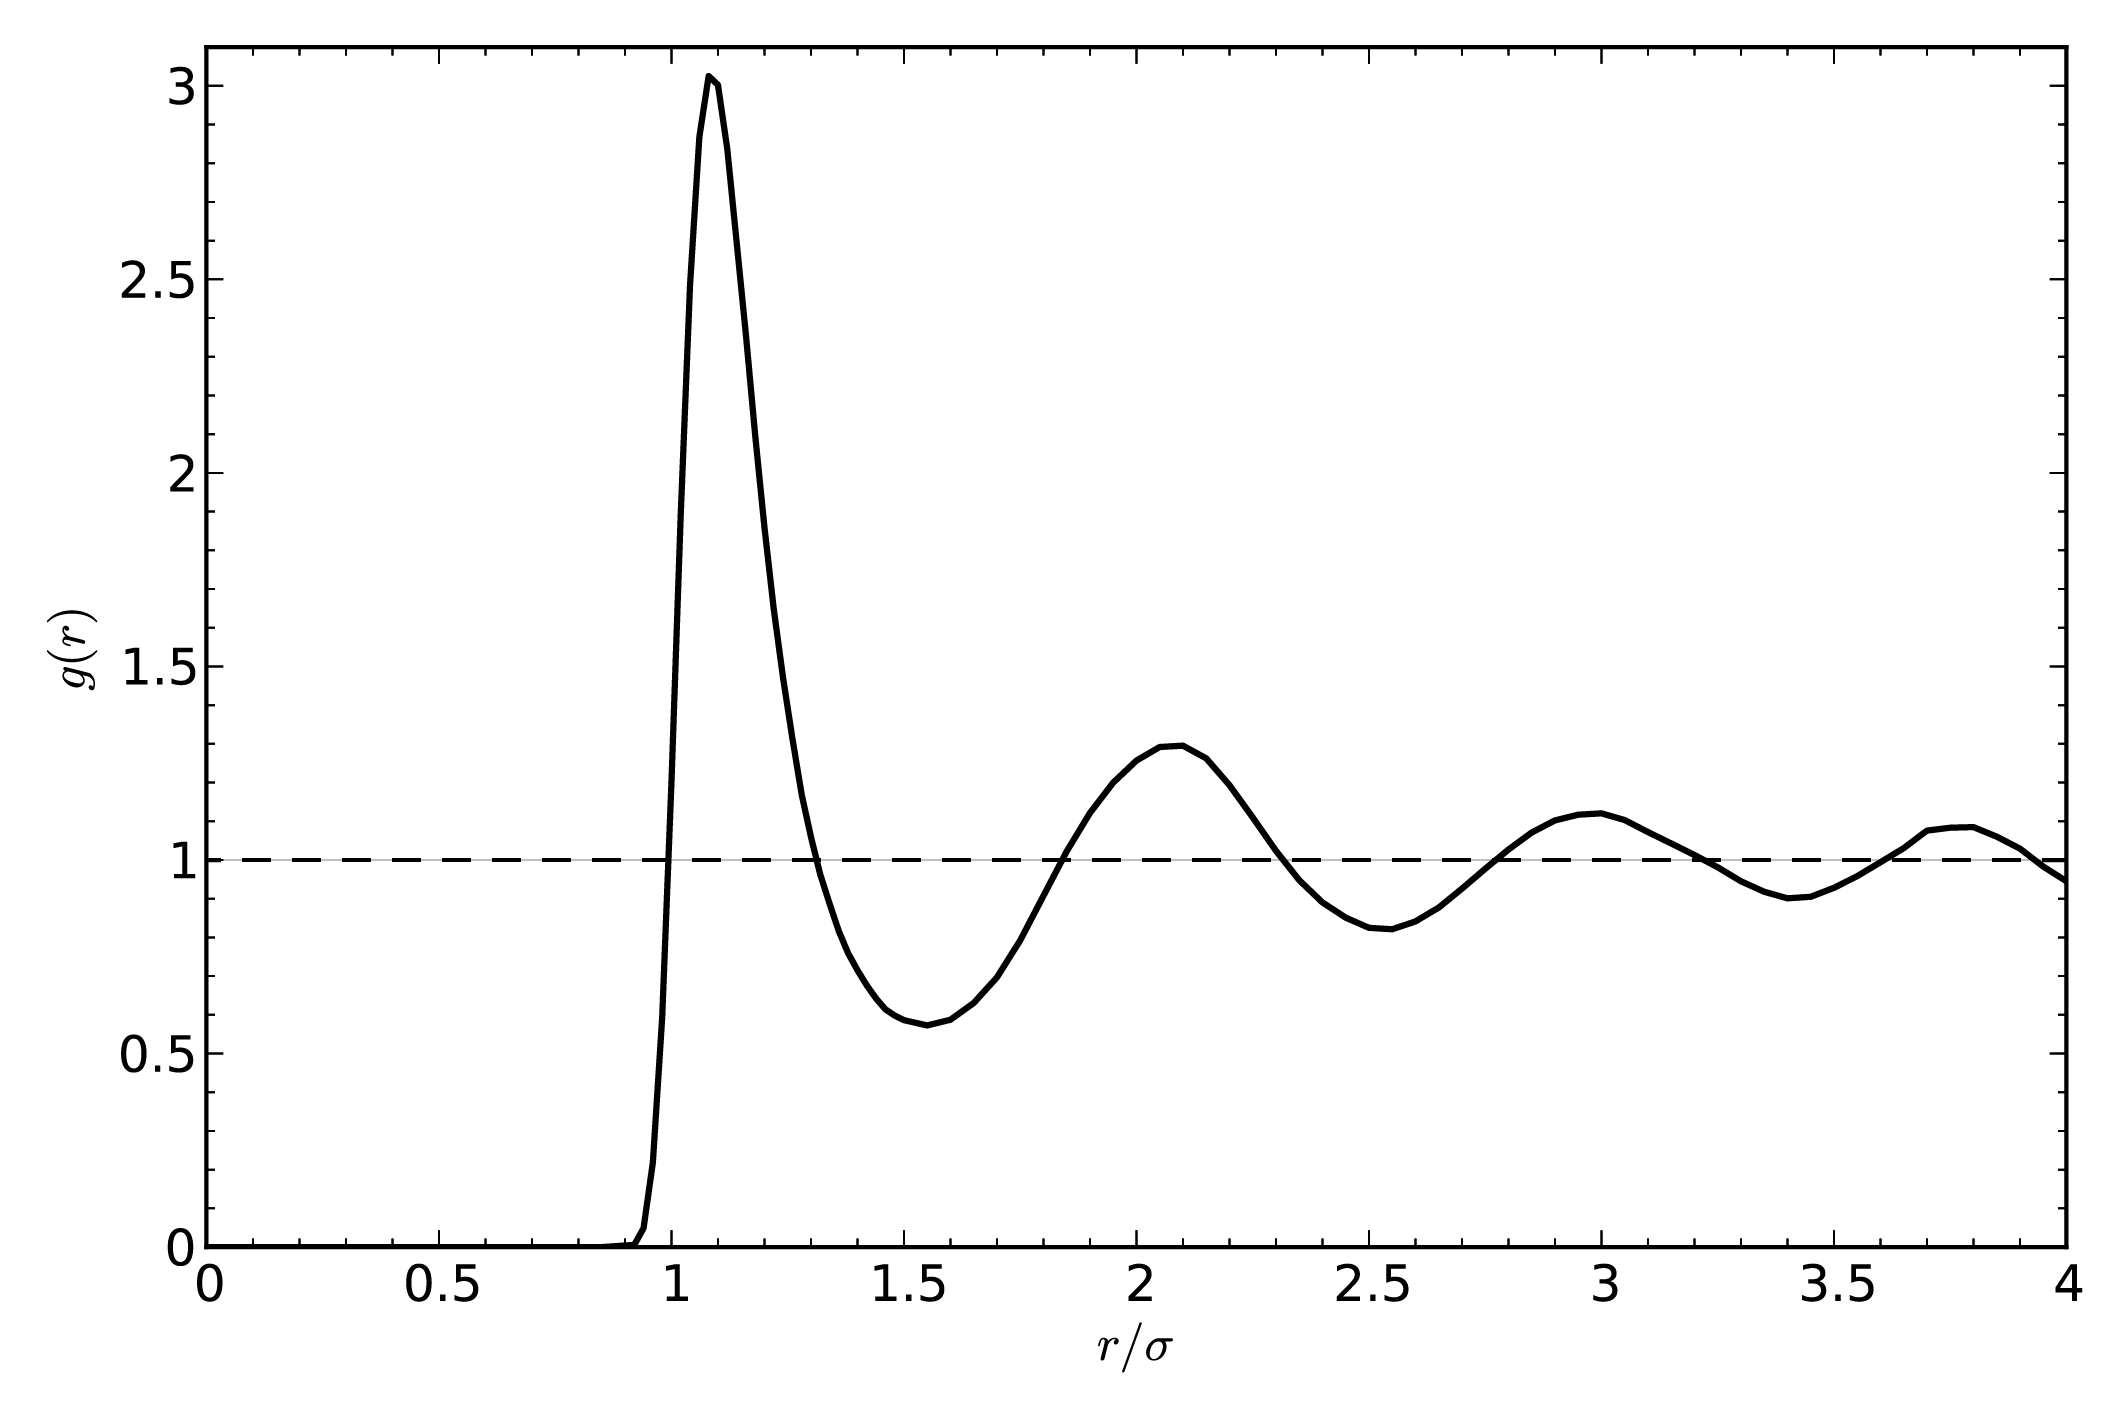
\includegraphics[width=\textwidth, trim=0cm 0cm 0cm 0cm, clip]{MD/figures/lennardjonesg_of_r.png}}
\label{fig:fcc_lattice_g_of_r}
\centering
\caption{The radial distribution function of an FCC lattice. The first peak reveals the distance between the face atoms and the corner atoms. Source: \url{http://en.wikipedia.org/wiki/Radial_distribution_function}.}
\end{figure}
The radial distribution function is defined as
\begin{align}
    \label{eq:g_of_r}
    g(r)dr &= \left\langle \sum_{i\neq j}\delta(r - |\vec r_i - \vec r_j|)\right\rangle{V\over N(N-1)4\pi r^2}\\
    &= {1 \over N} \left\langle \sum_{i\neq j}\delta(r - |\vec r_i - \vec r_j|)\right\rangle
\end{align}
where $N$ is seen as a normalization factor making sure that $\lim r\rightarrow \infty = 1$. A numerical implementation would loop over all relevant atom pairs, calculate their relative distance $r_{ij}$ and create a histogram over such distances. We would have to normalize each histogram bin by the volume of spherical shell as in \eqref{eq:g_of_r} with $dr\rightarrow \Delta r$ since each bin has a radial thickness. An implementation in $c++$ is given in  listing \ref{lst:g_of_r}.

\begin{lstlisting}[caption=Calculation of $g(r)$., label=lst:g_of_r]
vector<double> calculate_g_of_r(System &system, int num_bins) {
    // Create empty array of num_bins bins to store g(r)
    vector<double> g_of_r(num_bins,0);
    int num_atoms = system.r.size();

    // Loop over all atom pairs and put their distance into bin
    for(int i=0; i<num_atoms-1; i++) {
        Vector3D &r1 = system.r[i];
        for(int j=i+1; j<num_atoms; j++) {
            Vector3D &r2 = system.r[j];
            double dr = (r1 - r2).length();
            int bin_index = (dr / r_max) * num_bins;
            g_of_r[bin_index]++;
        }
    }

    // Normalize each bin
    for(int bin_index=0; bin_index<num_bins; bin_index++) {
        double r_inner = r_max * double(bin_index) / num_bins;
        double r_outer = r_max * double(bin_index+1) / num_bins;
        double r = 0.5*(r_inner + r_outer);
        double dr = r_outer - r_inner;

        double shell_volume = 4*M_PI*pow(r,2.0)*dr;
        double density = num_atoms/system.volume;
        g_of_r[bin_index] /= shell_volume * (num_atoms-1) * density;
    }

    return g_of_r;
}
\end{lstlisting}
The example code has complexity $N^2/2$, but since $g(r)$ is interesting only for relatively small $r$, we can improve the algorithm substantially by creating neighbor lists for each atom before looping over all relevant pairs. Experimentally, it is possible to measure the radial distribution function through diffraction experiments. By firing a beam of electrons or neutrons at the crystal, the electrons will be diffracted in different directions depending on the crystallic structure. One can measure the angles and intensities of the diffracted beams and then measure what is called \textit{structure factor} given by
\begin{align}
    S(\vec q) = {1\over N}\left\langle \sum_{jk} e^{-i\vec q(\vec R_j - \vec R_i)}\right \rangle,
\end{align}
where $\vec q$ is the spatial frequency (reciprocal coordinate), $N$ the number of atoms and $\vec R_{ij}$ the position of particles $i$ and $j$ respectively. We will not go into more detail in what the structure factor is other than that it is related to $g(r)$ through
\begin{align}
    S(q) = 1 + 4\pi\rho\frac{1}{q}\int dr r\sin(qr)[g(r) - 1],
\end{align}
if we assume that the material is isotropic\cite{kittel1996introduction}. The $g(r)$ can then be found through the inverse fourier transform
\begin{align}
    g(r) = 1 + {1\over 2\pi^2\rho r} \int dq(S(q) - 1)q\sin(qr).
\end{align}

\section{Diffusion constant}
The diffusion constant $D$ is defined by using the Einstein relation
\begin{align}
    \langle \Delta r^2 \rangle = 2dDt,
\end{align}
where $t$ is time, $d$ is the number of spatial dimensions and $\langle \Delta r^2 \rangle$ is average square displacement 
\begin{align}
    \langle \Delta r^2 \rangle = {1 \over N} \sum_{n=1}^N |\vec r(t) - \vec r(0)|^2.
\end{align}
In three dimensions, the diffusion constant is then found as
\begin{align}
    D = {\langle \Delta r^2 \rangle\over 6t}.
\end{align}
This is a fairly simple calculation, but in the MD-simulation, we need to keep track of how far each atom has moved from its initial position. A simple implementation is given in listing \ref{lst:diffusion}.
\begin{lstlisting}[caption=Calculation of the diffusion constant., label=lst:diffusion]
double calculate_diffusion_constant(System &system) {
    double rSquared = 0;
    for(int atom_index=0; atom_index<system.num_atoms; atom_index++) {
        double dr2 = (system.r[atom_index] - system.r0[atom_index]).length_squared();
        rSquared += dr2;
    }
    rSquared /= system.num_atoms; // Normalize to get <r^2>
    double diffusion_constant = rSquared / (6*system.t);
    return diffusion_constant;
}
\end{lstlisting}

  \end{chapter}

  \begin{chapter}{Implementation}
  \label{chap:md_implementation}
    \section{Implementation}

\subsection{Periodic boundary conditions}

\subsection{Two-body forces}
\label{sec:md_implementation_two_body_forces}
The Lennard-Jones potential gives rise to a two-body force acting only on pairs of atoms. In principle, this means we have to sum over all pairs in the system which for $n$ atoms in the system is $O(n^2)$. This calculation can be reduced to $O(n)$ by realizing that the gradient of the potential (hence the force) is nearly zero at $r \approx 2.5\sigma$, see figure \ref{fig:md_lennard_jones_2}. \todo{Show lennard jones force instead}
\begin{figure}[h]
\begin{center}
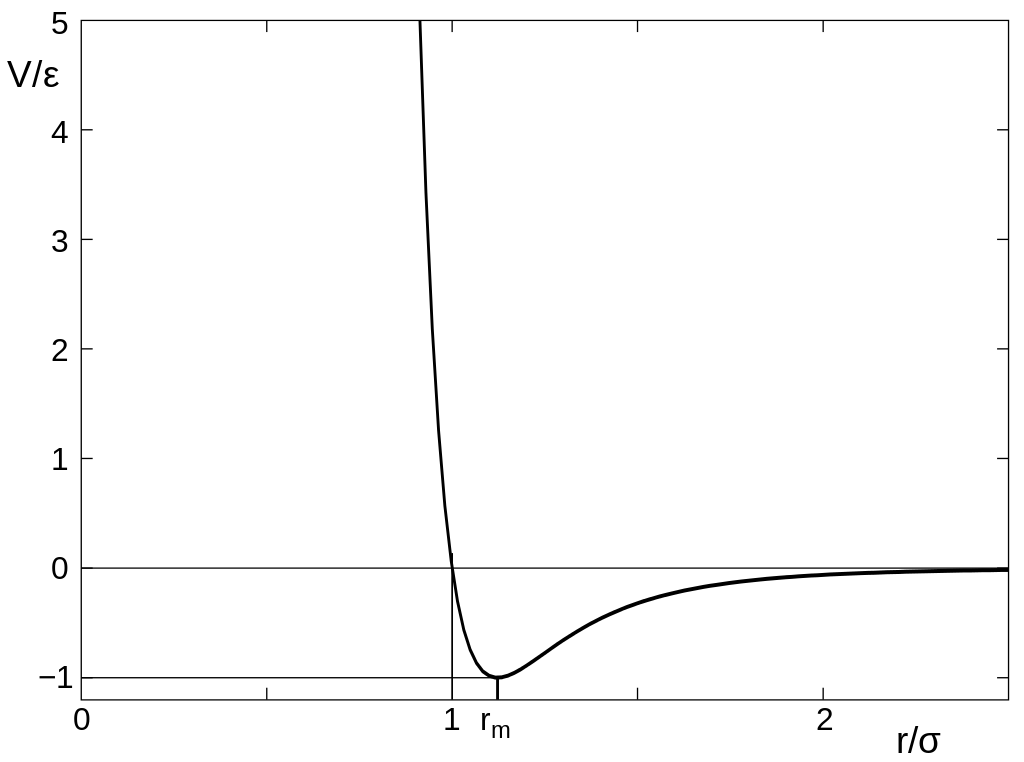
\includegraphics[width=1.0\textwidth, trim=0cm 0cm 0cm 0cm, clip]{MD/figures/lennard_jones.png}
\end{center}
\caption{The Lennard-Jones force. We see that the force is nearly zero at $r\approx 2.5\sigma$, so we don't need to calculate forces between atoms separated by a distance larger than $r_\text{cut} \equiv 2.5\sigma$.}
\label{fig:md_lennard_jones_2}
\end{figure}
We now introduce a certain cut-off distance $r_{cut}$ which we choose as the distance where the force is nearly zero, and set the force to be zero for any $r>r_{cut}$. The force between a pair of atoms $F(r_{ij})$ is then written as
\begin{align}
	F(r_{ij}) = \left\{\begin{array}{cc}
		F_{LJ}(r_{ij}) & \text{if } r \leq r_{cut}\\
		0 & \text{if } r > r_{cut}.
	\end{array}
	\right.
\end{align}
where $F_{LJ}$ is the standard Lennard-Jones force from eq \eqref{eq:md_lj_force}. We now don't need to sum over atom pairs of which the relative distance is larger than $r_cut$, so the calculation of forces is then globally $O(N)$. 
    \section{Parallelization}
\label{sec:md_parallelization}
Da parallelization technique is straight-up similar ta what tha fuck our phat asses did up in DSMC up in section \ref{sec:dmsc_parallelization}. Da spatial domain is divided tha fuck into $P_x\times P_y\times P_z$ smalla domains ($P_i$ bein tha number of processors up in tha $i$th dimension). Each such domain is then of size $l_x\times l_y \times l_z$ where $l_i = L_i/P_i$. Da processor arrangement n' labelin is done as shown up in figure \ref{fig:md_parallelization_2}, where a processor wit coordinates $(p_x, p_y, p_z)$ controls atoms wit coordinates up in tha range
\begin{align}
	\nonumber
	x&\in[p_xl_x, (p_x+1)l_x\rangle\\
	\nonumber
	y&\in[p_yl_y, (p_y+1)l_y\rangle\\
	z&\in[p_zl_z, (p_z+1)l_z\rangle.
\end{align}
\begin{figure}[h!]
\begin{center}
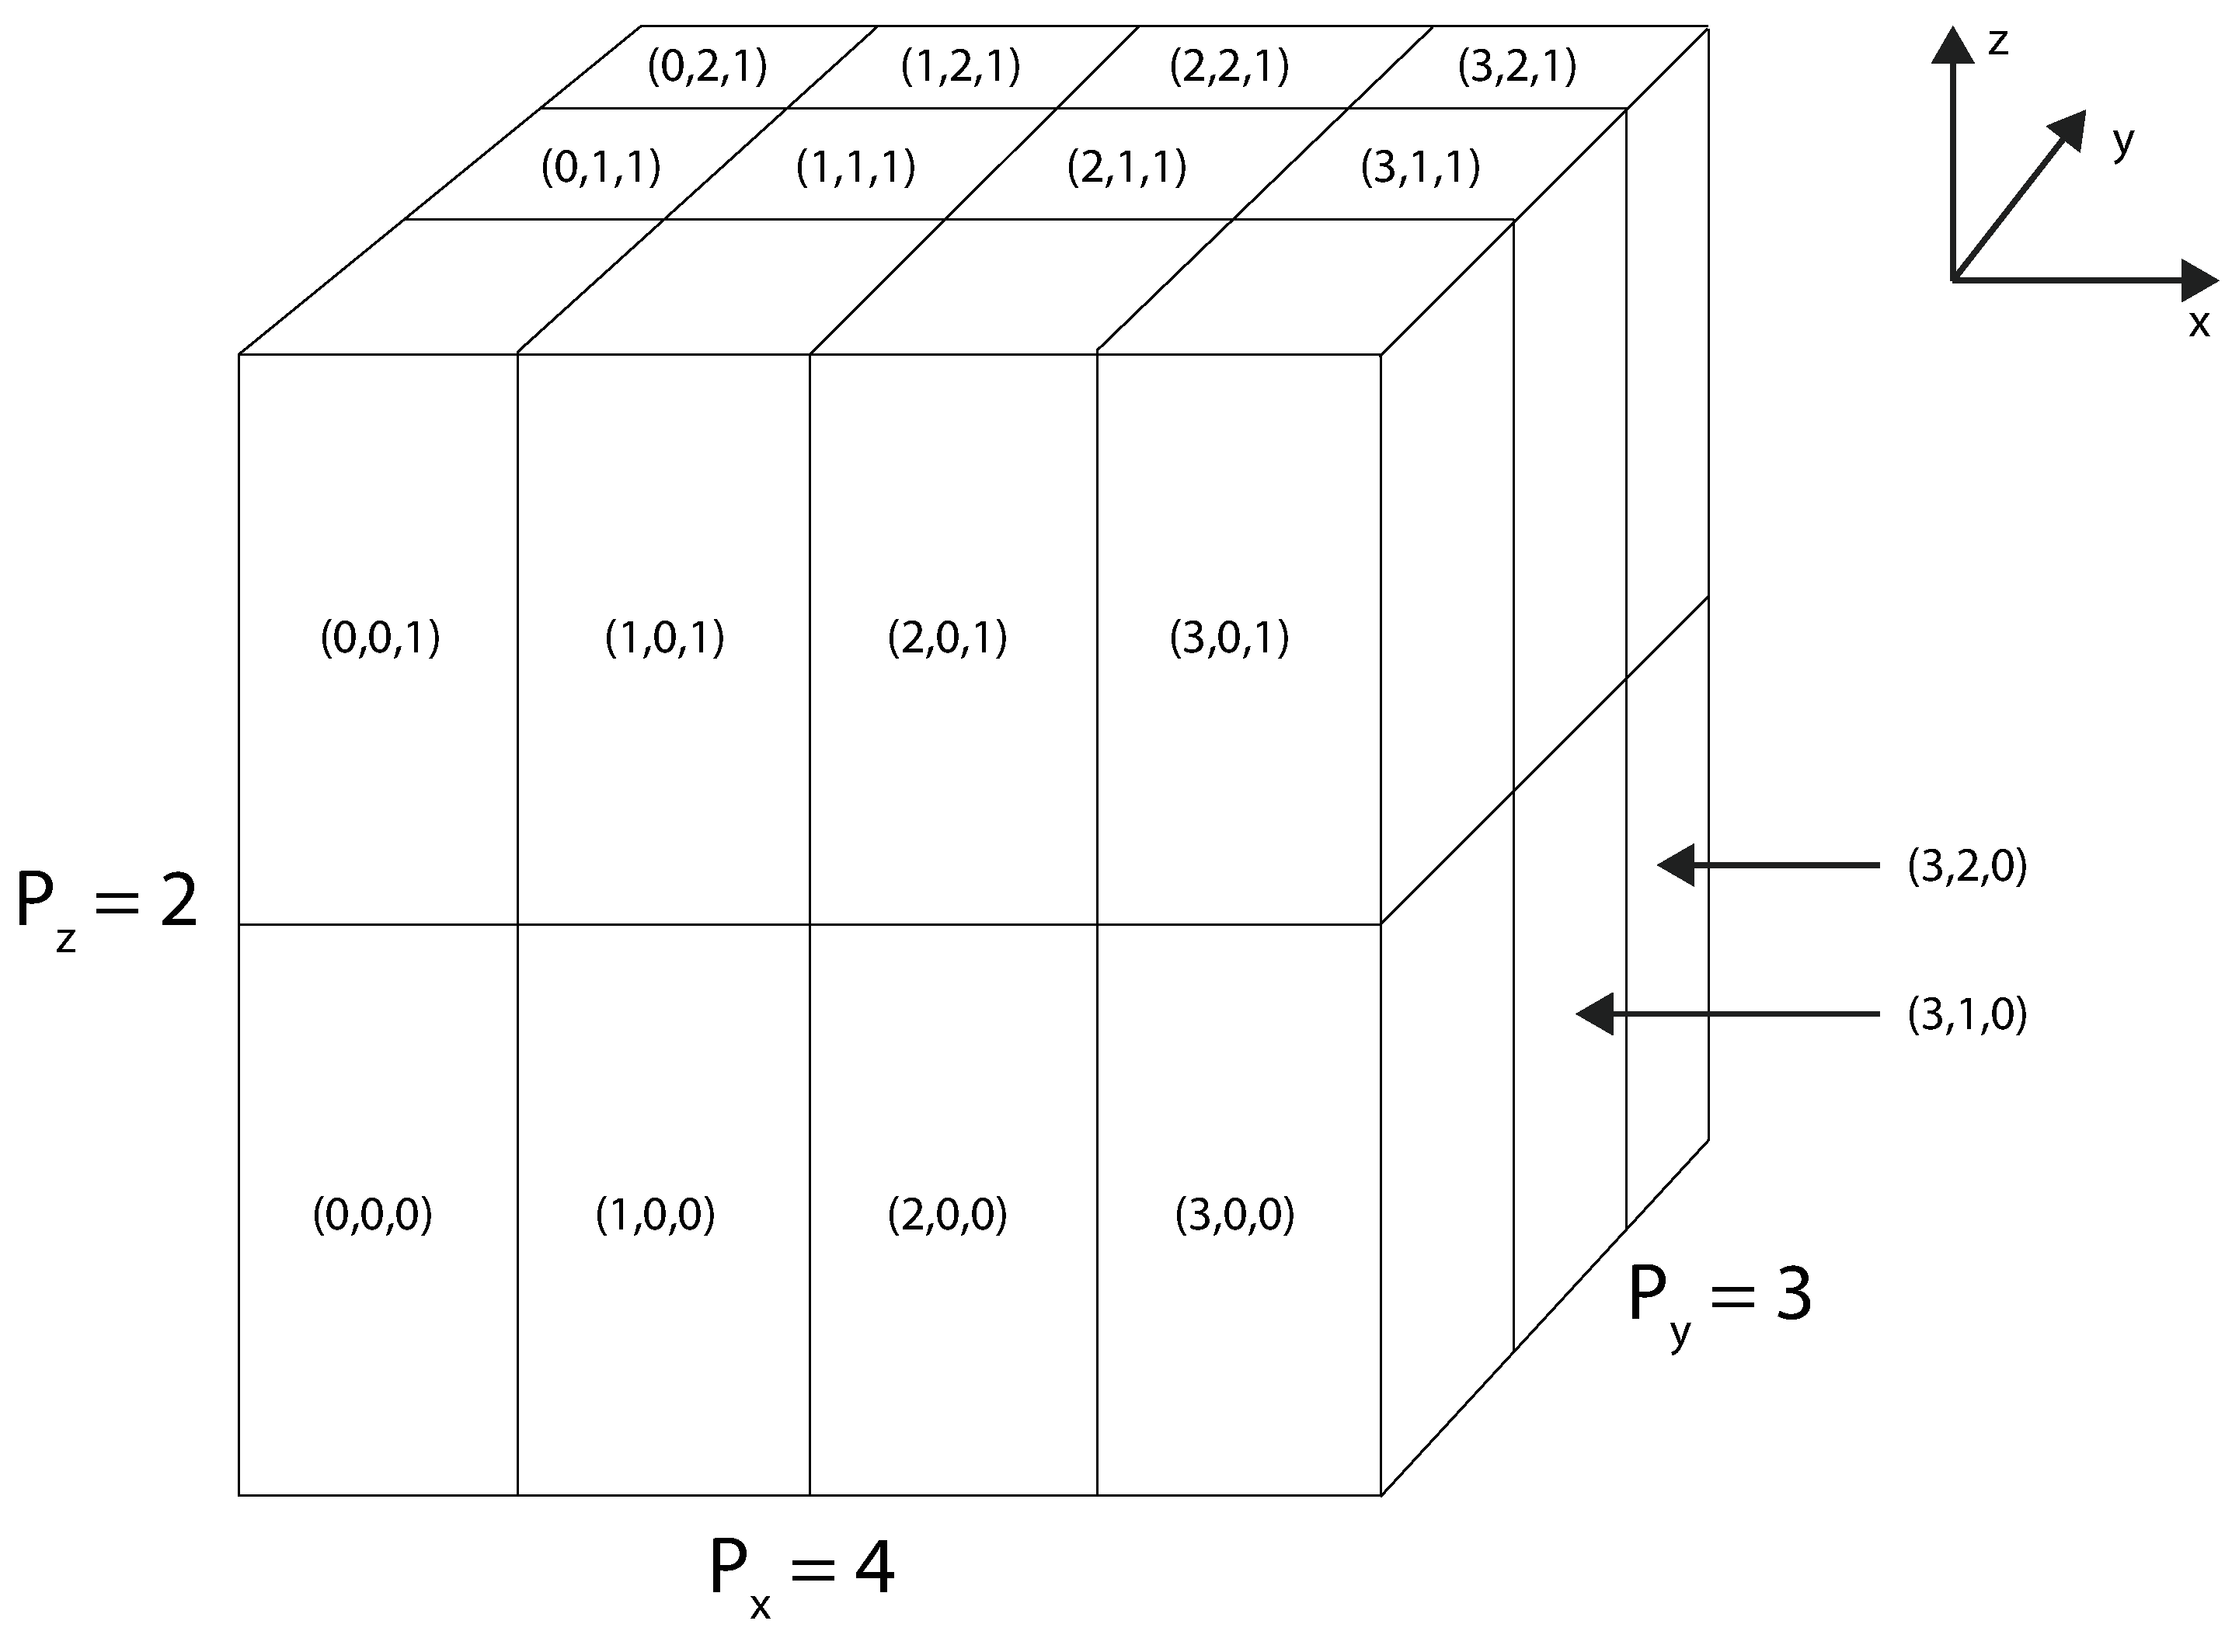
\includegraphics[width=0.7\textwidth, trim=0cm 0cm 0cm 0cm, clip]{DSMC/figures/parallelization_node_configuration.eps}
\end{center}
\caption{Processor labelin up in a 3-dimensionizzle grid. Y'all KNOW dat shit, muthafucka! Each processor is uniquely identified all up in its coordinizzle $(p_x, p_y, p_z)$.}
\label{fig:md_parallelization_2}
\end{figure}
We represent tha coordinatez of a atom on processor $(p_x, p_y, p_z)$ up in tha local coordinizzle system where tha CPUz origin $\vec p_\text{origin}$ defines tha coordinizzle system fo' realz. An atom wit global coordinates $\vec r$ will then have local coordinates $\vec r'$
\begin{align}
	\vec r' = \vec r - \vec p_\text{origin}.
\end{align}
We can then easily detect if a atom has moved outside its processorz domain by checkin if any of tha local coordinizzle components is outside tha range $[0, l_i)$ fo' dimension $i$. If a atom has moved ta another processor, it has moved ta one of tha 26 neighborin processors. Us thugs will use tha same 3-step process as busted lyrics bout up in subsection \ref{sec:dsmc_parallelization_exchange_particles} which is dopest illustrated wit tha 2-dimensionizzle example up in figure \ref{fig:md_parallelization_facet_technique}.
\begin{figure}[h!]
\begin{center}
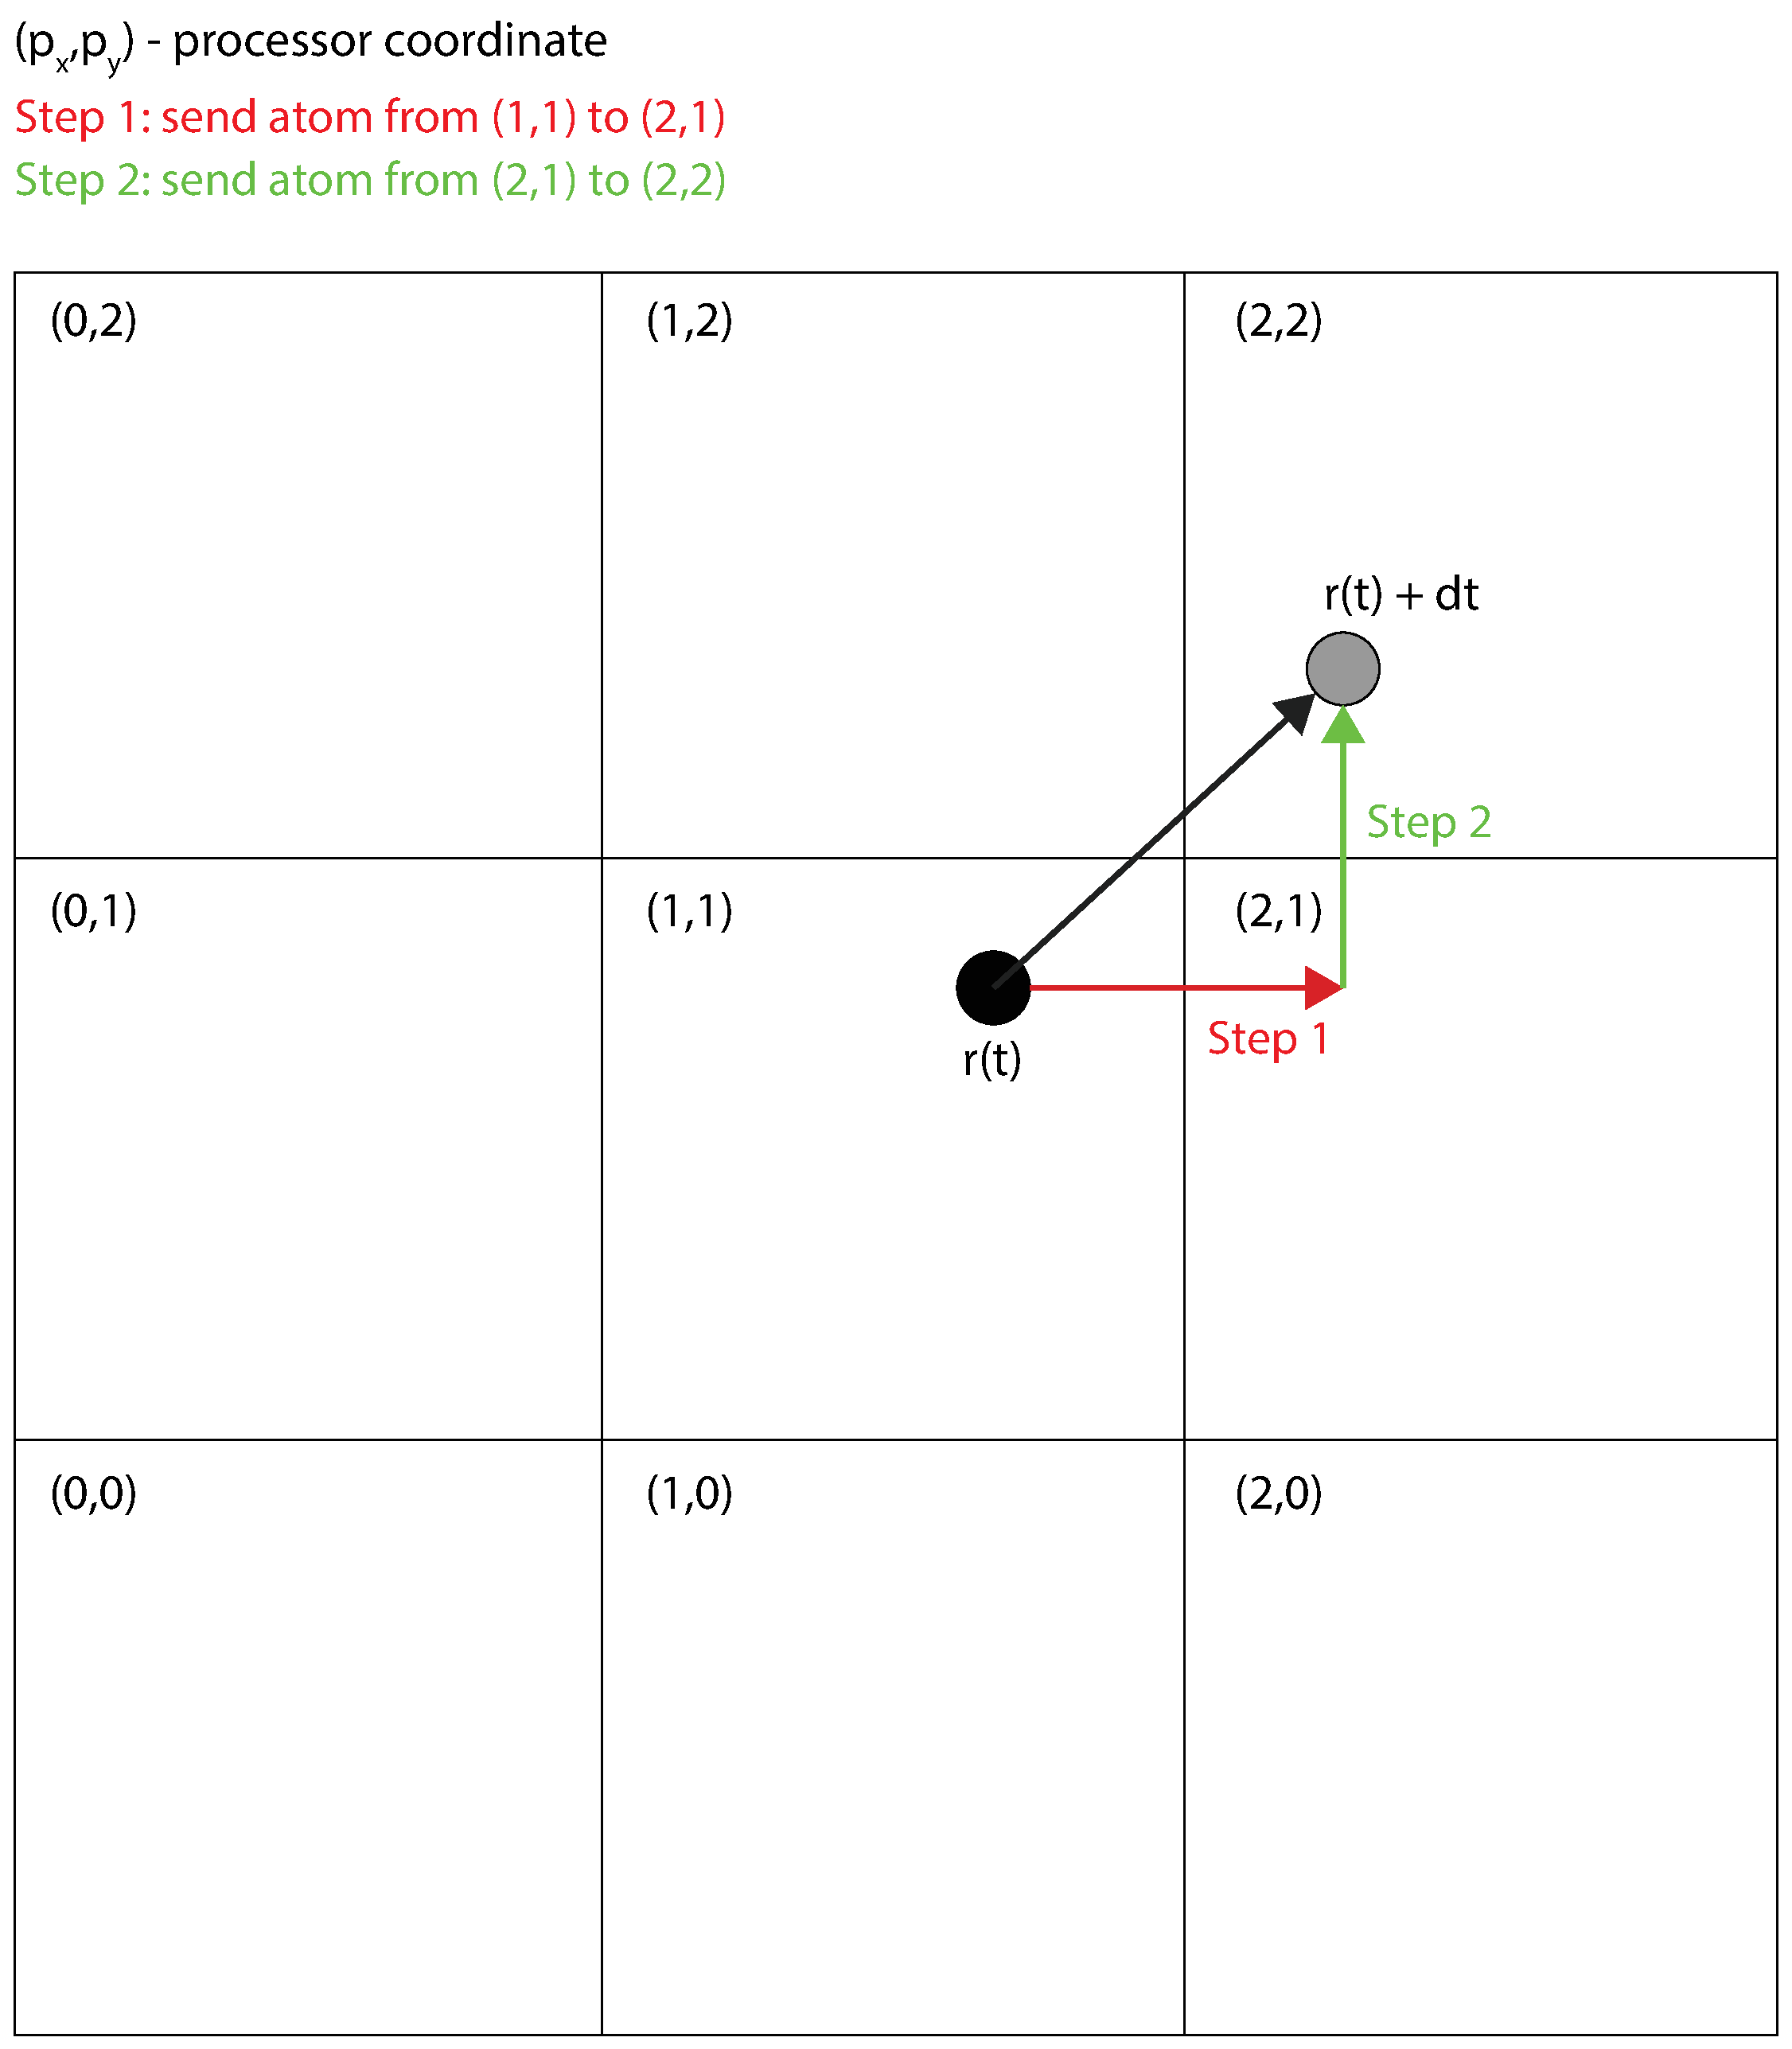
\includegraphics[width=0.7\textwidth, trim=0cm 0cm 0cm 0cm, clip]{MD/figures/parallelization_facet_technique.eps}
\end{center}
\caption{Da middle node (1,1) has 8 neighbors it need ta rap with. Each node only need ta rap wit its nearest neighbors (4 up in two dimensions, 6 up in three dimensions), cuz tha nearest neighbors can work as intermediate shiznit carriers fo' realz. An atom movin from processor (1,1) ta (2,2) will up in step 1 be busted ta (2,1), then up in step 2 be busted ta (2,2).}
\label{fig:md_parallelization_facet_technique}
\end{figure}
We only need ta know bout tha 6 nearest neighbors on each processor. Shiiit, dis aint no joke. We notice a neat detail here, periodic boundary conditions is automatically taken care of. If we again n' again n' again peep figure \ref{fig:md_parallelization_2}, our crazy asses have 4 processors up in tha $x$-direction. I aint talkin' bout chicken n' gravy biatch. Da processor ta tha \textit{right} of $(3,0,1)$ is $(0,0,1)$ if we use periodic boundary conditions. But since we use tha local coordinates on each processor, when a atom moves ta another processor, its coordinates must be \textit{shifted} so its has erect local coordinates on tha freshly smoked up processor. Shiiit, dis aint no joke. Each processor has one \textit{shift vector} per neighbor, containin tha transformation it need ta apply on tha atomz coordinates before it moved. Y'all KNOW dat shit, muthafucka! If tha atom moved all up in tha system boundary (periodic boundary conditions), tha shift vector must of course reflect all dis bullshit. 
    \section{System initialization}
\label{sec:md_system_init}
We are now ready to initialize the MD system. We assume that we will simulate an system with volume 
\begin{align}
	V=L_xL_yL_z,
\end{align}
where $L_i$ is the system size in the $i$th dimension. The system contains $N$ argon atoms and is performed on
\begin{align}
	P = P_xP_yP_z 
\end{align}
processors, $P_i$ being the number of processors in the $i$th dimension. Each processor controls a volume 
\begin{align}
	V_p = l_xl_yl_z,
\end{align}
where $l_i = L_i/P_i$ is the node length. The origin of processor $(p_x, p_y, p_z)$ is given as
\begin{align}
 	\vec p_\text{origin}(p_x, p_y, p_z) = p_xl_x\hat i + p_yl_y\hat j + p_zl_z \hat k.
\end{align}
The initialization process consists of creating the atoms, place them at some position and give them velocities according to the Maxwell-Boltzmann distribution (equation \eqref{eq:maxwell_boltzmann_vector_probability}). We will initially place the atoms on an face-centered cubic lattice (FCC lattice).
\subsection{FCC lattice}
The FCC lattice is a lattice structure where we place atoms on all 8 corners of a cube in addition to all the faces, hence the name. In figure \ref{fig:md_fcc} we see how the atoms are placed on the FCC lattice.
\begin{figure}[h!]
\begin{center}
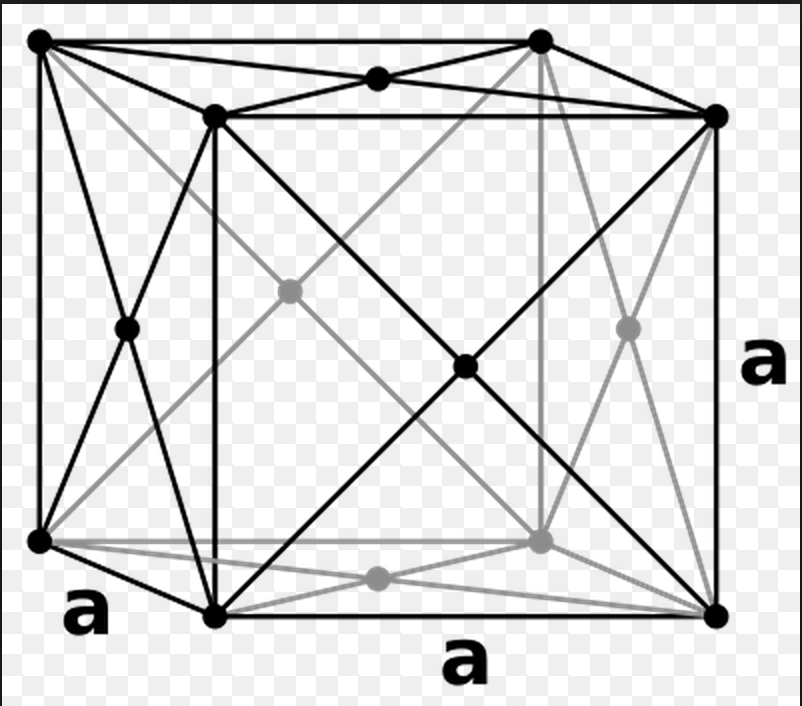
\includegraphics[width=0.7\textwidth, trim=0cm 0cm 0cm 0cm, clip]{MD/figures/fcc.png}
\end{center}
\caption{The face-centered cubic lattice. There are atoms on all eight corners of a cube, in addition to the six faces. The length $a$ is called the lattice constant. (Image from \url{http://en.wikipedia.org/wiki/File:Lattice_face_centered_cubic.svg}, accessed 19 March, 2014.)}
\label{fig:md_fcc}
\end{figure}
An FCC lattice can be constructed from a unit cell consisting of four atoms with local positions (relative to the origin of the unit cell)
\begin{align}
	\vec r_1 &= 0\ihat + 0 \jhat + 0 \khat\\
	\vec r_2 &= \frac{a}{2}\ihat + \frac{a}{2} \jhat + 0 \khat\\
	\vec r_3 &= 0\ihat + \frac{a}{2} \jhat + \frac{a}{2} \khat\\
	\vec r_4 &= \frac{a}{2}\ihat + 0 \jhat + \frac{a}{2} \khat,
\end{align}
where $a$ is the lattice constant, the length of the unit cell. By adding several such unit cells, each with origin determined by the unit cell coordinate $(m,n,l)$
\begin{align}
	\vec r_\text{unit cell} = ma\ihat + na\jhat + la\khat,
\end{align}
we can create a system of arbitrary size. Each atom is assigned a random velocity according to the Maxwell-Boltzmann distribution. The total number of atoms in the system is based on how many unit cells we create. If we label the number of unit cells \textit{per processor} in the $i$th dimension $N_c^{(i)}$, the total number of unit cells is
\begin{align}
	N_c = N_c^{(x)}N_c^{(y)}N_c^{(z)} P,
\end{align}
which gives the total number of atoms (each unit cell contains 4 atoms)
\begin{align}
	N = 4N_c.
\end{align}
The system size is then
\begin{align}
	L_x &= aN_c^{(x)}P_x\\
	L_y &= aN_c^{(y)}P_y\\
	L_z &= aN_c^{(z)}P_z,
\end{align}
yielding a total volume $V = a^3N_c$. In listing \ref{lst:md_fcc_lattice}, we have shown how this is implemented in C{}\verb!++!.
\begin{lstlisting}[caption=Code example showing how to create an FCC lattice on one of the processors., label=lst:md_fcc_lattice]
void create_fcc_lattice() {
    double xCell[4] = {0, 0.5, 0.5, 0};
    double yCell[4] = {0, 0.5, 0, 0.5};
    double zCell[4] = {0, 0, 0.5, 0.5};

    int index = 0;
    double velocity_standard_deviation = sqrt(boltzmann_constant*temperature/mass);
    for(int x = 0; x < unit_cells_per_cpu_x; x++) {
        for(int y = 0; y < unit_cells_per_cpu_y; y++) {
            for(int z = 0; z < unit_cells_per_cpu_z; z++) {
                // Loop over the 4 atoms in this unit cell
                for(int k = 0; k < 4; k++) {
                    positions.at(index).x = (x+xCell[k]) * FCC_a;
                    positions.at(index).y = (y+yCell[k]) * FCC_a;
                    positions.at(index).z = (z+zCell[k]) * FCC_a;
                    velocities.at(index).x = rnd.nextGauss()*velocity_standard_deviation;
                    velocities.at(index).y = rnd.nextGauss()*velocity_standard_deviation;
                    velocities.at(index).z = rnd.nextGauss()*velocity_standard_deviation;
                    index++; // Increase atom counter
                }
            }
        }
    }
}
\end{lstlisting}
This is the whole initialization process. The atoms are where they should be, they have a statistically correct velocity and we are ready to integrate forward in time.
    \section{Timestep}
We are using the Velocity Verlet algorithm as we discussed in section \ref{sec:md_time_integration}. The timestep calculation starts by what we called a half kick, where the velocities are integrated half a timestep with forward Euler. But to be able to do so, we need to have calculated the forces. This part is the most technical in the whole algorithm, because of two things. We need to find a way to implement the cut-off radius so that we don't loop over too many atom pairs, and each processor needs to have information about the atoms on its neighboring atoms (there are forces between atoms living on different CPUs). We will first discuss how duplicates of atoms, so-called ghost atoms, are copied between nodes before we explain how we use cell lists to compute forces between nearby atoms only. 
\subsection{Ghost atoms}
Assume now that we are going to calculate the forces between the atoms on some node with coordinates $(p_x, p_y, p_z)$. The atoms near the boundary will of course feel the presence of the atoms on the next processor (if they are sufficiently near). The node will then, from each of its 26 neighbors, get a copy of the atoms that are less than $r_\text{cut}$ from the node boundary. In figure \ref{fig:md_ghost_atoms}, this is illustrated in a two-dimensional example.
\begin{figure}[h]
\begin{center}
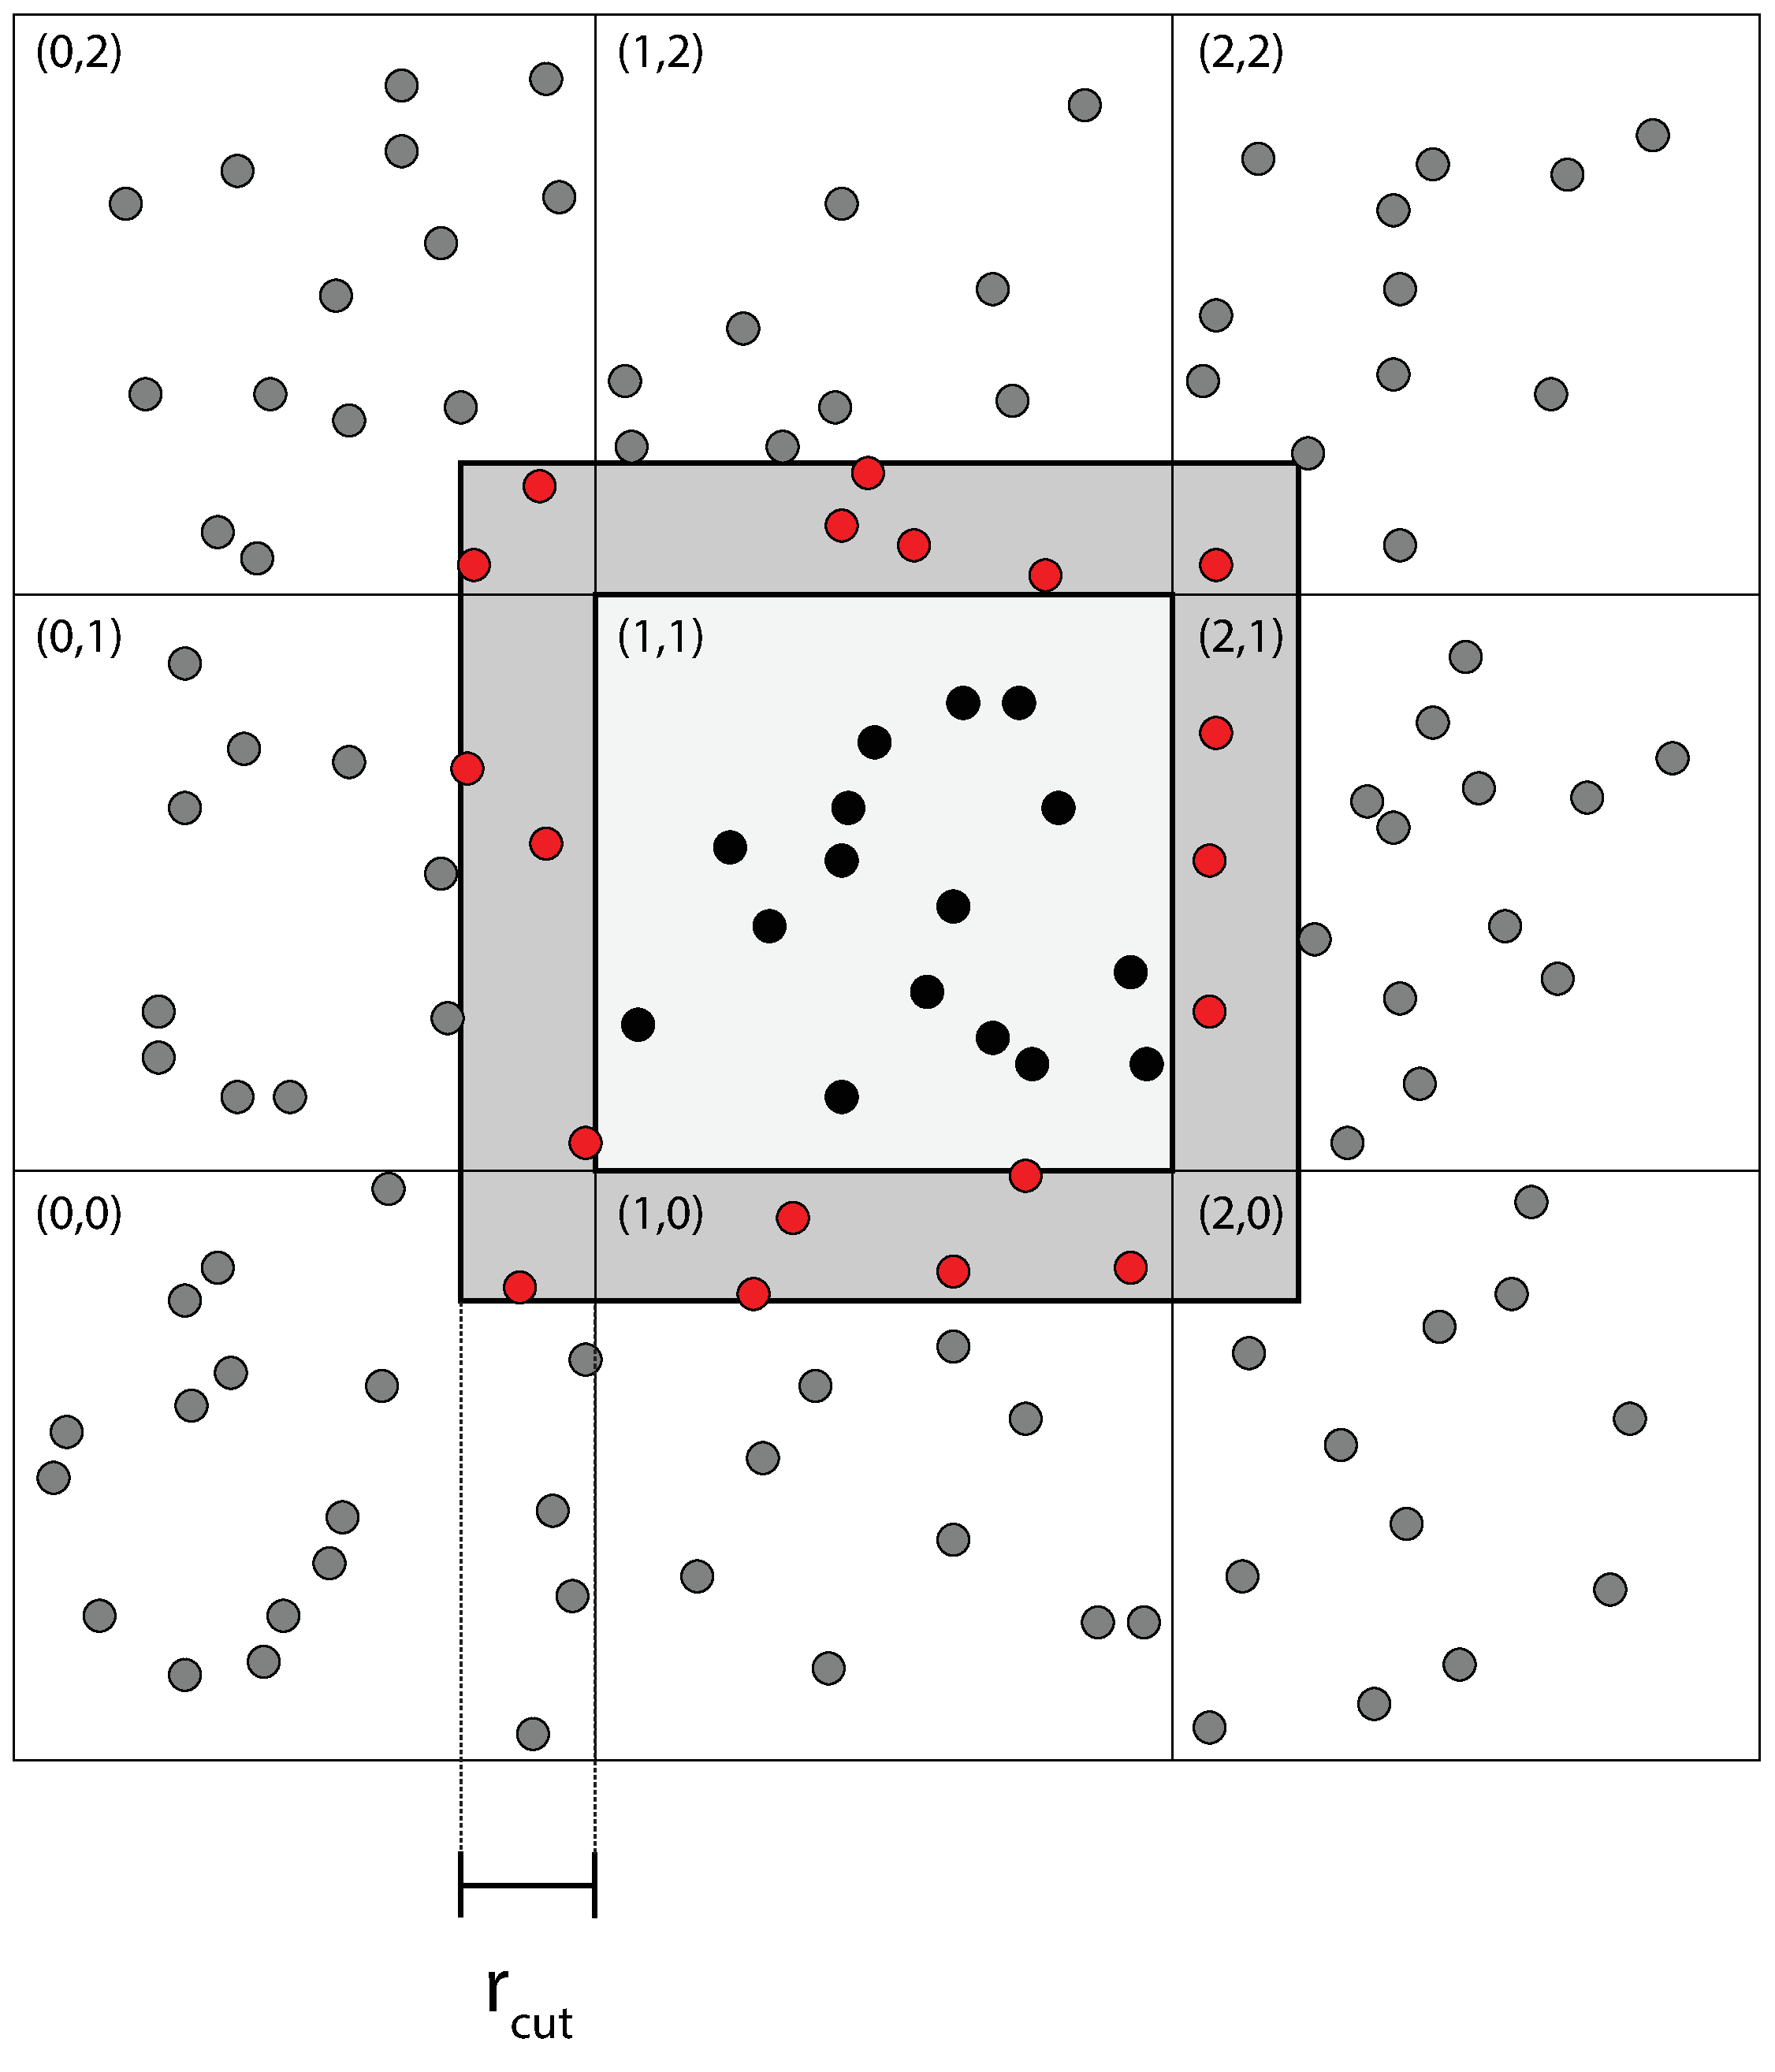
\includegraphics[width=0.8\textwidth, trim=0cm 0cm 0cm 0cm, clip]{MD/figures/parallelization_ghost_atoms.eps}
\end{center}
\caption{The middle processor with coordinates (1,1) in a two-dimensional system recieves a copy of all the atoms less than $r_\text{cut}$ from the boundary (ghost atoms, marked red) from the neighboring eight processors. The gray area is the region with the ghost atoms. The black dots are the atoms on node $(1,1)$, gray dots are atoms that do not contribute to the forces of the black atoms.}
\label{fig:md_ghost_atoms}
\end{figure}
Since we don't calculate forces between atoms displaced by more than the cut-off radius, we actually compute all the forces we want. This process is done for every processor, every timestep, so that all nodes have all the information they need to compute the forces (and potential energy).
\subsection{Cell lists}
We will now sort the atoms on a node into cells, similar to the collision cells in DSMC (see section \ref{sec:dsmc_implementation_timestep}). Each processor has atoms with coordinates in the range $[0, l_i)$, $l_i$ being the node length in the $i$th dimension, and ghost atoms with coordinates $(-r_\text{cut}, 0) \cup [l_i, l_i + r_\text{cut})$. We choose the cells to be about the same size as the cut-off radius, which gives the number of such cells $N_f$ (force cells) in the $i$th dimension
\begin{align}
	N_f = \ceil{l_i / r_\text{cut}} + 2,
\end{align}
where we have added two extra \textit{ghost cells} containing the ghost atoms, $\ceil{a}$ is the ceiling function of $a$, that is, the smallest integer number not larger than $a$. The reason we use the ceiling function is so the length of the node exactly matches the combined length of the cells (minus the two extra ghost cells). The size of the cells is then at least $r_\text{cut}$ so that the atoms within a cell will not feel the presence of atoms from any other cells than the 26 nearest neighbors. In figure \ref{fig:md_cells} we have illustrated the idea in a two-dimensional system. We see the total spatial domain of a processor with the copied ghost atoms (in the gray area), divided into cells of size $r_\text{cut}$. The yellow cell will compute forces between all of its atoms and the atoms in the green cells. This is done for every inner cell (the ghost atoms are computed on another processor).
\begin{figure}[h]
\begin{center}
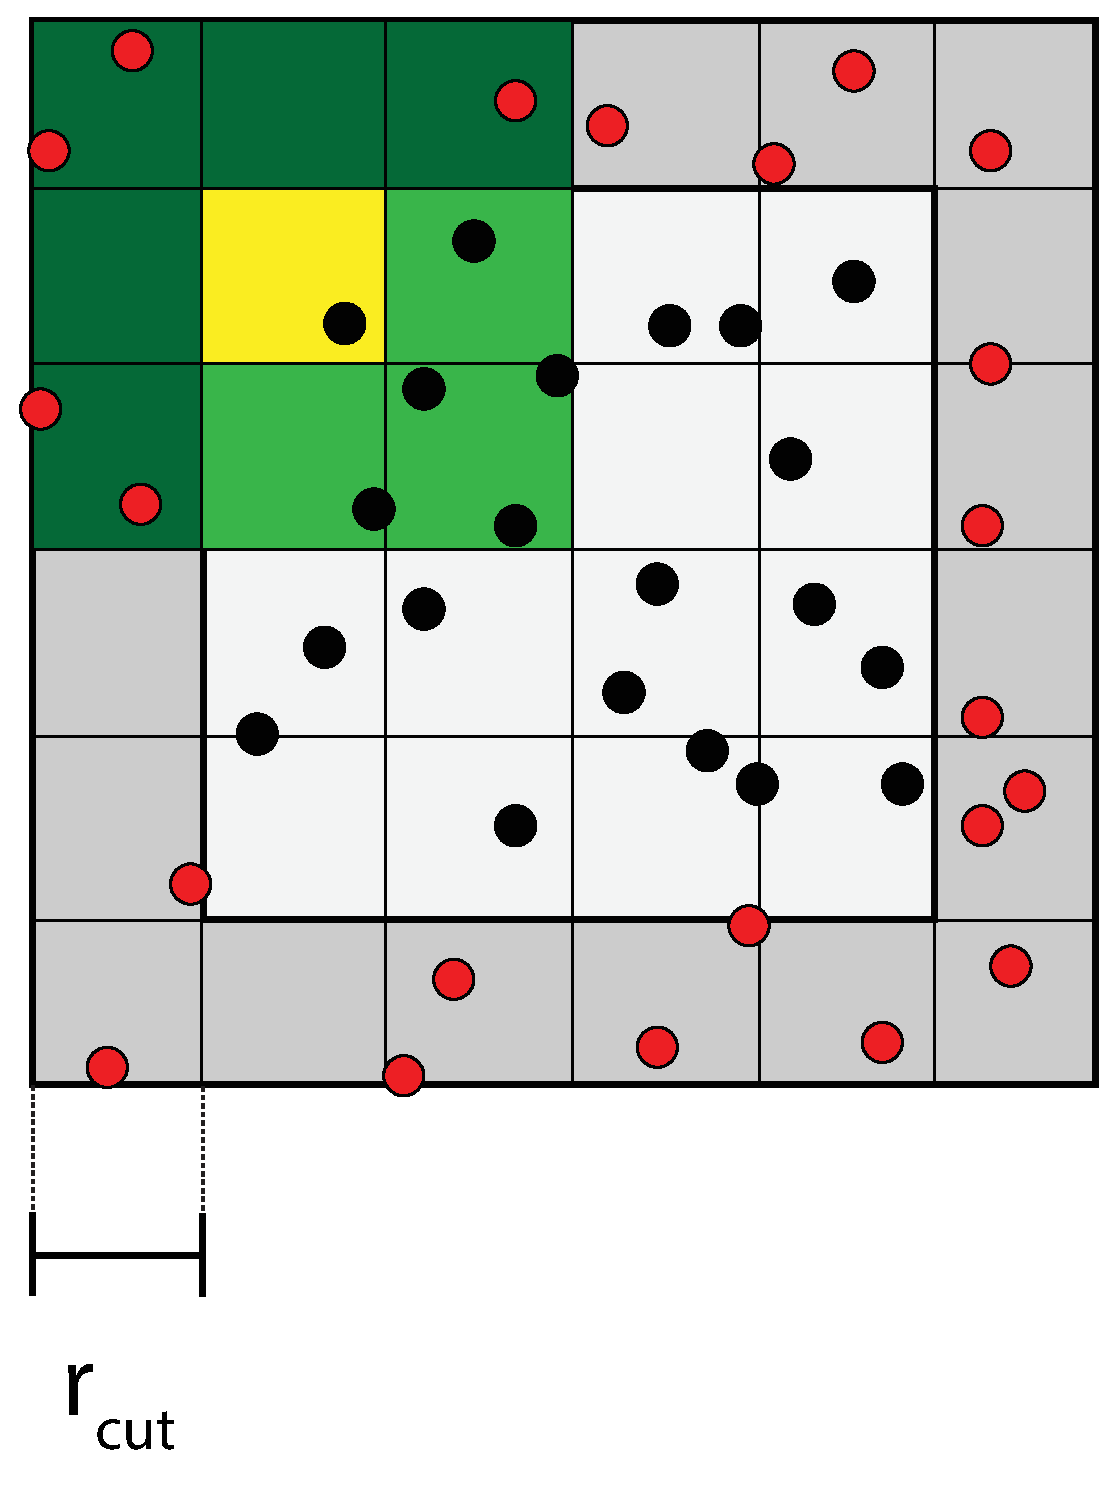
\includegraphics[width=0.8\textwidth, trim=0cm 0cm 0cm 0cm, clip]{MD/figures/cells.eps}
\end{center}
\caption{The spatial domain for a processor with the added ghost atoms in the gray area. The domain is divided into cells of size $r_\text{cut}$ so that the yellow cell only needs to compute forces between atoms in the cell and the neighboring 8 green cells. The processor will only process the cells (the ghost atoms are computed on another processor).}
\label{fig:md_cells}
\end{figure}
\subsection{Calculation of forces}
The atoms are now sorted into cells. We then loop over all cells, and for each cell, loop over the 26 neighboring cells. With each cell pair, loop over all pairs of atoms and calculate forces between them if their relative distance is smaller than $r_\text{cut}$. In the inner scope of the loop, we now have two atoms $i$ and $j$ with positions $\vec r_i$ and $\vec r_j$. Given their relative distance $\vec r_{ij} = (\Delta x, \Delta y, \Delta z)$, we are ready to compute the force between them. The Lennard-Jones force is given as (for $r_{ij} \leq r_\text{cut}$)
\begin{align}
	\vec F(\vec r_{ij}) = -24\epsilon\left[2\left(\frac{\sigma^{12}}{r_{ij}^{13}}\right) - \left(\frac{\sigma^6}{r_{ij}^7}\right)\right]\vec u_{ij},
\end{align}
and if we choose the so-called MD units ($\sigma = 1.0, \epsilon = 1.0$, see appendix \ref{app:physical_units}), the $x$-component of the force is given as
\begin{align}
	\label{eq:md_implementation_timestep_lj}
	F_x(r_{ij}) = -24\left[\left(\frac{2}{r_{ij}^{12}}\right) - \left(\frac{1}{r_{ij}^6}\right)\right]\frac{\Delta x}{r_{ij}^2},
\end{align}
where $\Delta x$ is the $x-$component of $\vec r_{ij}$. Notice that we have factored out $1/r_{ij}^2$. This is arithmetical convenient for the implementation, because, as we see in equation \eqref{eq:md_implementation_timestep_lj}, we need $r_{ij}^{-6}$ and $r_{ij}^{-12}$, which both are easily calculated from $r_{ij}^{-2}$ as powers.\\
First, we skip atoms displaced by a distance larger than $r_\text{cut}$ and compute the square of the relative distance
\begin{align}
	r_{ij}^2 = \left|\vec r_i - \vec r_j\right|^2.
\end{align}
Its inverse is gives us the higher powers
\begin{align}
	r_{ij}^{-2} &= \frac{1}{r_{ij}^2}\\
	r_{ij}^{-6} &= \left(r_{ij}^{-2}\right)^3\\
	r_{ij}^{-12} &= \left(r_{ij}^{-6}\right)^2.
\end{align}
In listing \ref{lst:md_lennard_jones} we have shown the code that calculates the Lennard-Jones force. We see that Newton's third law is implemented by skipping a pair of atoms if \classname{atom\_index\_0}<\classname{atom\_index\_1}, avoiding calculating that pair twice. 
\begin{lstlisting}[caption=Implementation of the Lennard-Jones force. The code loops over all cells and their neighbors computing the forces between all the atoms in neighboring cells., label=lst:md_lennard_jones]
void calculate_lennard_jones() {
    // Loop through all local cells (not including ghosts)
    for (int cell_index_x=1; cell_index_x<=num_cells.x; cell_index_x++) {
    for (int cell_index_y=1; cell_index_y<=num_cells.y; cell_index_y++) {
    for (int cell_index_z=1; cell_index_z<=num_cells.z; cell_index_z++) {
    // Index of this cell
    cell_index = cell_index_from_ijk(cell_index_x, cell_index_y, cell_index_z);

    // Loop through all neighbors (including ghosts) of this cell.
    for (int i=cell_index_x-1; i<=cell_index_x+1; i++) {
    for (int j=cell_index_y-1; j<=cell_index_y+1; j++) {
    for (int k=cell_index_z-1; k<=cell_index_z+1; k++) {
    // Index of neighbor cell
    cell_index_2 = cell_index_from_ijk(i,j,k);
    // Head is pointing to the first atom index in a cell
    int atom_index_0 = head_atoms[cell_index]; 

    while (atom_index_0 != EMPTY) { // The last atom in a cell points at the EMPTY value
    int atom_index_1 = head_atoms[cell_index_2]; // Index of atom j
    while (atom_index_1 != EMPTY) {
        if(atom_index_0 < atom_index_1) { // Newton's 3rd law
            double dx = positions.at(atom_index_0).x-positions.at(atom_index_1).x;
            double dy = positions.at(atom_index_0).y-positions.at(atom_index_1).y;
            double dz = positions.at(atom_index_0).z-positions.at(atom_index_1).z;
            
            double dr2 = dx*dx + dy*dy + dz*dz;

            if (dr2<r_cut_squared) {
                double dr2_inverse = 1.0/dr2;
                double dr6_inverse = dr2_inverse*dr2_inverse*dr2_inverse;
                double dr12_inverse = dr6_inverse*dr6_inverse;
                double force = 24*(2*dr12_inverse-dr6_inverse)*dr2_inverse;

                accelerations.at(atom_index_0).x += force*mass_inverse*dx;
                accelerations.at(atom_index_0).y += force*mass_inverse*dy;
                accelerations.at(atom_index_0).z += force*mass_inverse*dz;

                accelerations.at(atom_index_1).x -= force*mass_inverse*dx;
                accelerations.at(atom_index_1).y -= force*mass_inverse*dy;
                accelerations.at(atom_index_1).z -= force*mass_inverse*dz;
            }
        }
        atom_index_1 = linked_list_of_atoms[atom_index_1]; // Next
    }
    atom_index_0 = linked_list_of_atoms[atom_index_0];
    }}}}}}}
}
\end{lstlisting}
    \section{Complex geometries}
As we did with DSMC, we want to study flow in arbitrary geometries.  To be able to do this, we need to create a model that satisfies some properties we already have in DSMC. The flowing fluid needs to
\begin{itemize}
	\item be confined in a subset of the total volume
	\item have realistic interactions with the solid wall
	\item have energy drained by the solid.
\end{itemize}
The first requirement is not completely strict, but most of the flowing fluid should be in the free volume. The reason why we need to drain the energy is that in order to induce fluid flow, we will apply a constant force that increases the total energy of the system. We want to reach an equilibrium where the average rate of drained energy exactly matches the energy from the applied force. We assume that the geometry is described as a boolean function $G : \mathcal(R)^3\rightarrow \{1,0\}$ that fully determines whether a point in space is part of the solid or the free volume. A convinient representation is the voxelization described in section \ref{sec:dsmc_binary_representation}. 
\subsection{A naive approach}
To illustrate the basic idea, we will discuss the simplest model satisfying only the first two requirements. Given a molecular dynamics state, we can loop through the positions $\vec r_i$ of each atom $i$, and mark the atoms as \textit{frozen} if $G(\vec r_i) = 1$ (which means that this point is part of the solid). Atoms marked as frozen will not move at all, but all forces are calculated normally. One way of interpreting the non-moving frozen atoms is that they have infinite mass. The total energy is still conserved in the system. An implementation is illustrated in listing \ref{lst:md_simple_solid}.

\begin{lstlisting}[caption=Example code showing how to mark atoms within a solid., label=lst:md_simple_solid]
bool point_is_a_solid(double *position) {
	int voxel_index_i = position[0] / system_length[0] * num_voxels[0];
	int voxel_index_j = position[1] / system_length[1] * num_voxels[1];
	int voxel_index_k = position[2] / system_length[2] * num_voxels[2];

	// The world matrix is a binary matrix
	return world_matrix[voxel_index_i, voxel_index_j, voxel_index_k];
}

void mark_frozen_atoms() {
	for(int i=0; i<num_atoms; i++) {
		double *position = positions[i];
		if(point_is_a_solid(position)) {
			atom_types[i] = FROZEN;
		}
	}
}

void move() {
	for(int i=0; i<num_atoms; i++) {
		if(atom_types[i] != FROZEN) {
			positions[i][0] += velocities[i][0];
			positions[i][1] += velocities[i][1];
			positions[i][2] += velocities[i][2];
		}
	}
}
\end{lstlisting}
If the atoms forming the solid are dense enough, very few atoms will be inside the wall, so the first requirement is satisfied. The interaction between the solid and the flowing fluid is as realistic as the potential is, so the only requirement not satisfied is the drainage of the energy. In figure \ref{fig:md_simplesolid}, we see how the red flowing atoms are confined within a cylinder with radius $R$. 

\begin{figure}[h]
\begin{center}
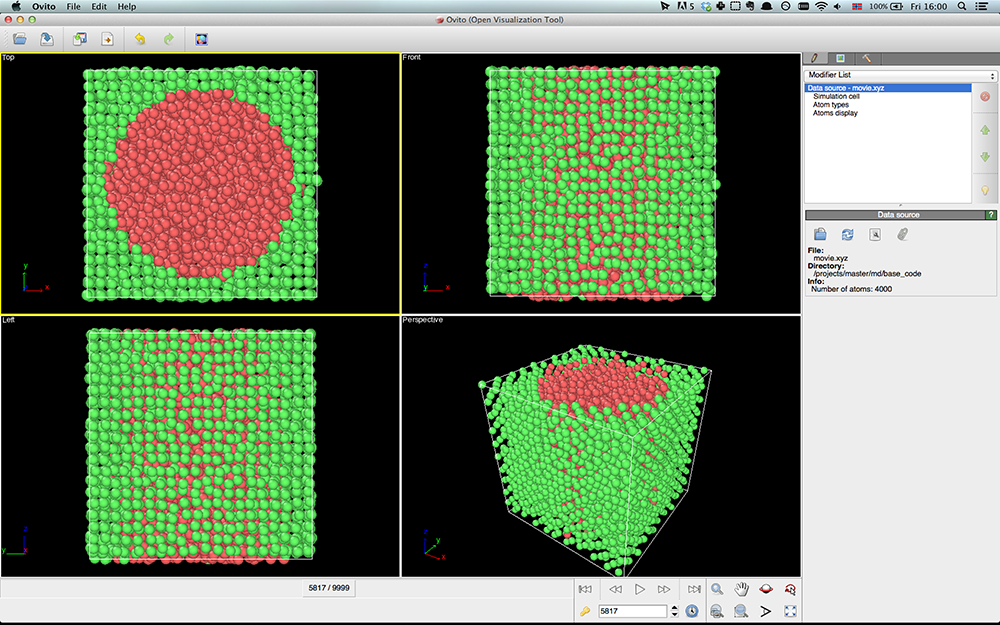
\includegraphics[width=1.0\textwidth, trim=0cm 0cm 0cm 0cm, clip]{MD/figures/solid_model.png}
\label{fig:md_simple_solid}
\end{center}
\caption{A simple model of a solid where the green atoms are frozen confining the red flowing atoms within a cylinder of radius $R$. The visualization is done in Ovito.}
\end{figure}

\subsection{A simple model of a solid}
We can improve the solid model by adding a harmonic oscillator potential to all the frozen atoms. Instead of freezing them completely, we allow them to vibrate around their equilibrium position $\vec q$ which is the initial position of the simulation. The force on atom $i$ in the solid is then
\begin{align}
	F^{(s)}(\vec r_i) = -k(\vec r_i - \vec q_i) 
	- \sum_{j\neq i} 24\epsilon\left[2\left(\frac{\sigma^{12}}{r_{ij}^{13}}\right) - \left(\frac{\sigma^6}{r_{ij}^7}\right)\right]\vec u_{ij},
\end{align}
where $k$ is the strength of the oscillator, $\vec q_i$ is the equilibrium position for atom $i$ and the last part is the Lennard-Jones potential described in section \ref{sec:md_lj_potential}.\\
\subsubsection{Energy drainage}
The energy is of course still conserved with this model, but we can now apply a thermostat on the atoms in the solid making them act as a large reservoir trying to keep the temperature at some wall temperature $T_w$. With this model, we can study flow in any geometry with a behaviour near that of the DSMC model. An implementation is shown in listing \ref{lst:md_ho_solid}.

\begin{lstlisting}[caption=Implementation of the harmonic oscillator model of a solid., label=lst:md_ho_solid]

void apply_gravity() {
    for(n=0;n<num_atoms;n++) {
        if(atom_type[n] != FROZEN) velocities[n][gravity_direction] += gravity_acceleration*dt;
    }
}

void apply_harmonic_oscillator() {
    double spring_constant = 1000.0;
    for(n=0; n<num_atoms; n++) {
        if(atom_type[n] == FROZEN) {
            double dx = positions[n][0] - initial_positions[n][0];
            double dy = positions[n][1] - initial_positions[n][1];
            double dz = positions[n][2] - initial_positions[n][2];
            accelerations[n][0] += -spring_constant*dx / mass;
            accelerations[n][1] += -spring_constant*dy / mass;
            accelerations[n][2] += -spring_constant*dz / mass;
        }
    }
}

void step() {
    move();
    apply_gravity();
    apply_lennard_jones();
    apply_harmonic_oscillator();
    update_velocities();
}
\end{lstlisting}
  \end{chapter}

  \begin{chapter}{Results}
  \label{chap:md_results}
    In this chapter we discuss the results of our MD simulations. Here we start by a scaling performance benchmark in section \ref{sec:md_benchmark} before we in section \ref{sec:md_cylinder_result} move on to a validation of the Knudsen correction we confirmed with the DSMC model. Most of the concepts are equivalent as in DSMC in section \ref{sec:dsmc_parallelization_performance}, so the reader is is assumed to have read that section.

\section{Parallelization performance}
\label{sec:md_benchmark}
The parallelization scheme we have used in MD is very similar to the one we used in DSMC. In section \ref{sec:dsmc_parallelization_performance}, we measured both the strong and the weak scaling efficiency ($\eta_s$ and $\eta_w$) which measure two different ways of scaling the program. We will not repeat the discussion about these except present the result for both scaling for the MD program. 

\subsection{Strong scaling}
The strong scaling efficiency $\eta_s$ tells us how well the program scales if we keep the system size constant while increasing the number of processors. The strong scaling efficiency was defined as
\begin{align}
	\eta_s = \frac{t_1}{Nt_N},
\end{align}
where $t_1$ is the total run time using one processor and $t_N$ is the total run time using $N$ processors. In this benchmark, we chose a system consisting of $48\times48\times48=110592$ unit cells which gives a total of 442368 atoms. When we increase the number of processors, these 48 unit cells per dimension are distributed on the processors. The timestep was $\Delta t = 0.02$ and the initial temperature was approximately $T_0=$\unit{100}{\kelvin} so that the final gas temperature was around $T=$\unit{60}{\kelvin}. This fall in temperature is explained by the fact that the FCC lattice is the potential minimum, so with a non-zero temperature, some of the initial kinetic energy will be converted to potential energy. We run the program with the number of processors in the range 1 to 512. In table \ref{tab:md_strong_scaling} we have presented the results for this benchmark which is summarized in figure \ref{fig:md_strong_scaling}. We see that when going from one to two processors, we get a more than ideal speedup with $\eta_s(N_\text{CPU}=2)=1.17$ which can be explained by the CPU cache. When a processor compute with a value stored at some memory address, it will first look in the three levels of cache to see if the value of the memory address is cached there. Cached values are much faster available for computation than those only in the memory. When going from one processor to two, a larger part of the positions array (which is used in the force calculation) can be cached, hence a more than double speedup is obtainable. When using a larger number of processors, the MPI communication time starts increasing so that the total time increases per cpu. 

\begin{table}[h]
\begin{center}
    \begin{tabular}{|l|l|l|l|l|}
    \hline
    $N_\text{CPU}$ & $N_\text{atoms}/N_\text{CPU}$ & $t_N$ & $\eta_s$ \\ \hline
    1 & 442368 & \unit{29196}{\second} & 1.00\\
    \hline
    2 & 221184 & \unit{12471}{\second} & 1.17\\
    \hline
    4 & 110592 & \unit{6435}{\second} & 1.13\\
    \hline
    8 & 55296 & \unit{3469}{\second} & 1.05\\
    \hline
    16 & 27648 & \unit{1926}{\second} & 0.95\\
    \hline
    32 & 13824 & \unit{1021}{\second} & 0.89\\
    \hline
    64 & 6912 & \unit{715}{\second} & 0.64\\
    \hline
    128 & 3456 & \unit{375}{\second} & 0.61\\
    \hline
    256 & 1728 & \unit{220}{\second} & 0.52\\
    \hline
    512 & 864 & \unit{150}{\second} & 0.38\\
    \hline
    \end{tabular}
    \caption{Benchmark results showing the strong scaling efficiency $\eta_s$ for the MD program. We see that when going from one to two processors, we get a more than ideal speedup with $\eta_s(N_\text{CPU}=2)=1.17$ which can be explained by the CPU cache. When a processor compute with a value stored at some memory address, it will first look in the three levels of cache to see if the value of the memory address is cached there. Cached values are much faster available for computation than those only in the memory. When going from one processor to two, a larger part of the positions array (which is used in the force calculation) can be cached, hence a more than double speedup is obtainable. When using a larger number of processors, the MPI communication time starts increasing so that the total time increases per cpu.}
    \label{tab:md_strong_scaling}
    \end{center}
\end{table}

\begin{figure}[h!]
\begin{center}
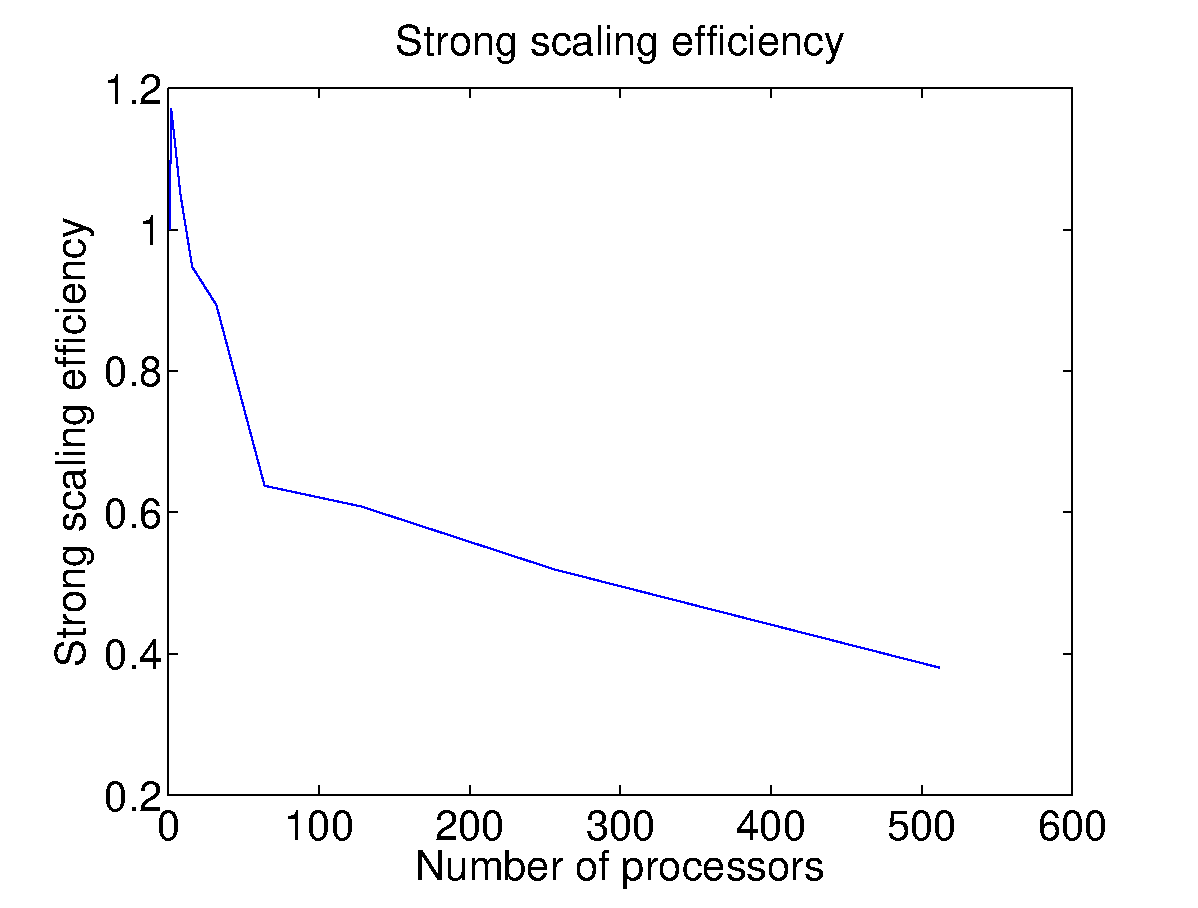
\includegraphics[width=0.7\textwidth, trim=0cm 0cm 0cm 0cm, clip]{MD/figures/strong_scaling.eps}
\end{center}
\caption{Benchmark results showing the strong scaling efficiency $\eta_s$ for the MD program. We see that when going from one to two processors, we get a more than ideal speedup with $\eta_s(N_\text{CPU}=2)=1.17$ which can be explained by the CPU cache. When a processor compute with a value stored at some memory address, it will first look in the three levels of cache to see if the value of the memory address is cached there. Cached values are much faster available for computation than those only in the memory. When going from one processor to two, a larger part of the positions array (which is used in the force calculation) can be cached, hence a more than double speedup is obtainable. When using a larger number of processors, the MPI communication time starts increasing so that the total time increases per cpu.}
\label{fig:md_strong_scaling}
\end{figure}

\subsection{Weak scaling}
If we increase the number of processors, but keep the nubmer of atoms per processor constant, we can use the weak scaling efficiency $\eta_w$ to see how the program scales in this case. The weak scaling efficiency is defined as
\begin{align}
	\eta_w = \frac{t_1}{t_N},
\end{align}
where again $t_1$ is the total run time using one processor and $t_N$ is the run time using $N$ processors. In this benchmark, we chose $10\times10\times10=1000$ unit cells per processor yielding a total of 4000 atoms per cpu. The timestep here as well is $\Delta t = 0.02$ with the same initial temperature as in the strong scaling so that the final temperature is approximately $T=$\unit{60}{\kelvin}. In table \ref{tab:md_weak_scaling} and figure \ref{fig:md_weak_scaling}, we have presented the results for the weak scaling. 

\begin{table}[h]
\begin{center}
    \begin{tabular}{|l|l|l|l|l|}
    \hline
    $N_\text{CPU}$ & $N_\text{atoms}$ & $t_N$ & $\eta_w$ \\ \hline
    1 & 4000 & \unit{1246}{\second} & 1.00\\
    \hline
    2 & 8000 & \unit{1278}{\second} & 0.97\\
    \hline
    4 & 16000 & \unit{1398}{\second} & 0.89\\
    \hline
    8 & 32000 & \unit{1441}{\second} & 0.86\\
    \hline
    16 & 64000 & \unit{1521}{\second} & 0.82\\
    \hline
    32 & 128000 & \unit{1620}{\second} & 0.77\\
    \hline
    64 & 256000 & \unit{1639}{\second} & 0.76\\
    \hline
    128 & 512000 & \unit{1735}{\second} & 0.72\\
    \hline
    256 & 1024000 & \unit{2027}{\second} & 0.61\\
    \hline
    512 & 2048000 & \unit{3379}{\second} & 0.37\\
    \hline
    \end{tabular}
    \caption{Benchmark results showing the weak scaling efficiency $\eta_w$ for the MD program. }
    \label{tab:md_weak_scaling}
    \end{center}
\end{table}

\begin{figure}[h!]
\begin{center}
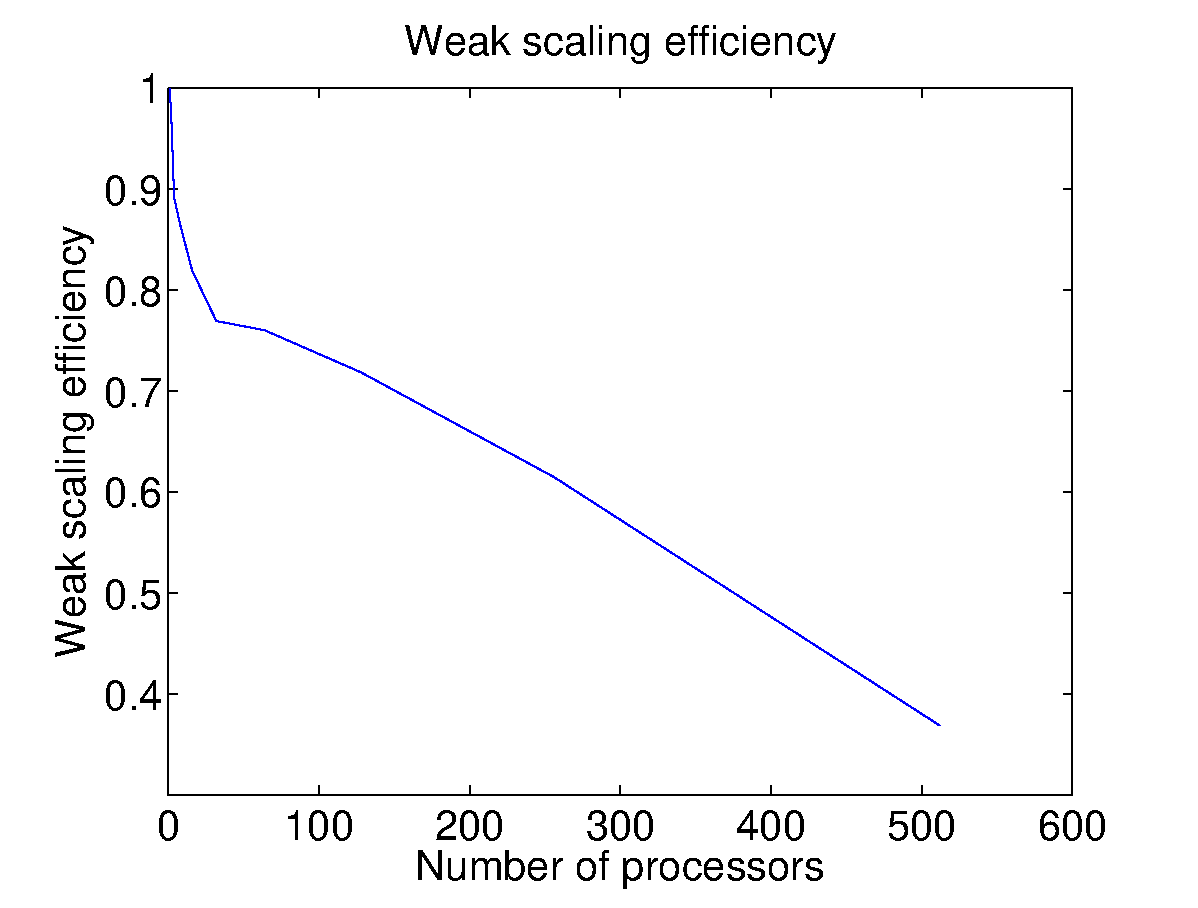
\includegraphics[width=0.7\textwidth, trim=0cm 0cm 0cm 0cm, clip]{MD/figures/weak_scaling.eps}
\end{center}
\caption{Benchmark results showing the weak scaling efficiency $\eta_w$ for the MD program.}
\label{fig:md_weak_scaling}
\end{figure}

\section{Flow in a cylinder, varying Knudsen number}
\label{sec:md_cylinder_result}
We have used the MD program to simulate flow in a cylinder with a fixed radius $R$, just like we did in section \ref{sec:results_for_simple_geometries} with DSMC. We will measure the permeability to see how well the Knudsen correction factor (see section \ref{sec:knudsen_correction}) predicts the permeability for very small pores (here a cylinder) with an atomic model. The cylinder was created with the solid model we described in section \ref{sec:md_simple_model_of_a_solid}. Since the solid now consists of atoms (in DSMC it was just a scalar field defining the surface), we should create the cylinder carefully. We have prepared the system with the following steps
\begin{itemize}
	\item Heat the system 2000 timesteps, $T=$\unit{300}{\kelvin}
	\item Thermalize the system 2000 timesteps
	\item Heat the system 2000 timesteps, $T=$\unit{300}{\kelvin}
	\item Thermalize the system 2000 timesteps
	\item Create cylinder (explained below)
	\item Reduce density (explained below).
\end{itemize}
By first heating the system, we let the system melt from a solid state to a liquid state. This allows the system to become more random than in the initial lattice. Once we create the cylinder, we apply a harmonic oscillator potential on the atoms in the cylinder so they more or less stay in their initial position. We have here chosen a system consisting of $64\times64\times64=262144$ unit cells which gives a total of 1048576 atoms to begin with. This in turn yields a system with size $L_i=336.64Å$ in the $i$th dimension. By choosing the cylinder radius to be $r=0.45L_i$ and the flow in the $z$-direction, we mark all atoms within a distance $r$ from the center (in the $xy$-plane) as gas atoms, and atoms outside $r$ as solid atoms. But the cut-off radius was chosen to be $r_\text{cut}=2.5\sigma$ (see section \ref{sec:md_implementation_two_body_forces}), so the gas atoms inside the cylinder will not feel the precense of the atoms outside $r+2.5\sigma$ directly. To save computation time, we have removed all atoms outside this radius. Such a cylinder is shown in figure \ref{fig:md_cylinder} where the yellow atoms are the solid wall wheras the green atoms are the gas.
\begin{figure}[h!]
\begin{center}
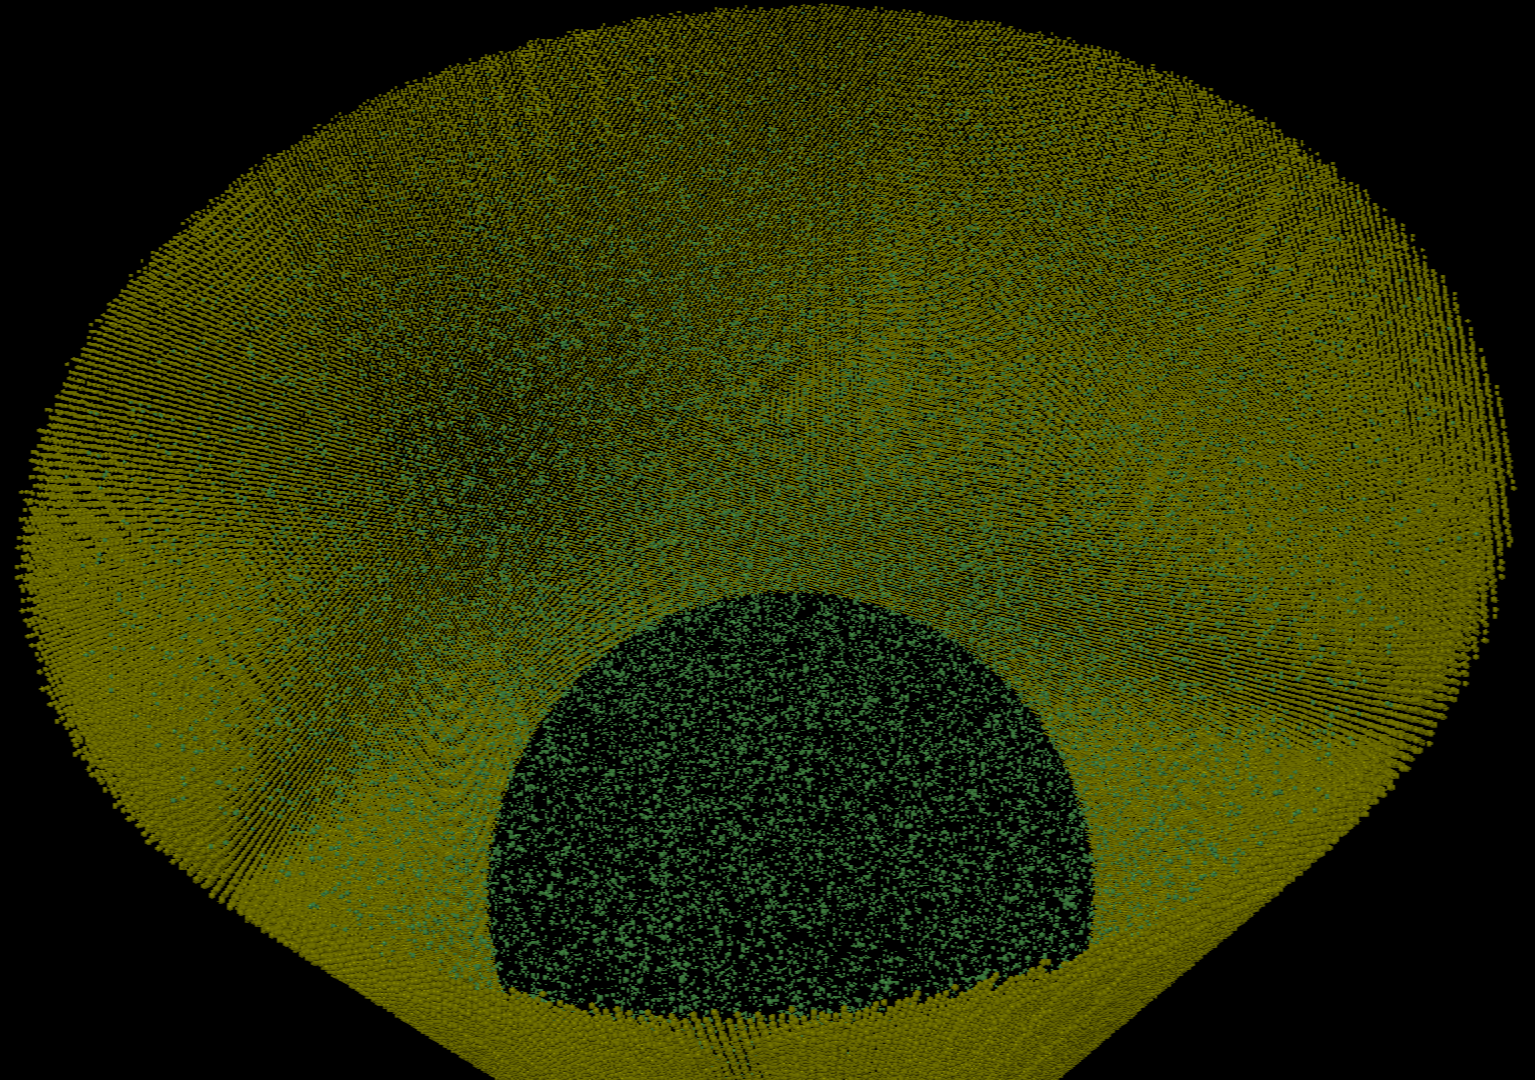
\includegraphics[width=0.8\textwidth, trim=0cm 0cm 0cm 0cm, clip]{MD/figures/md_cylinder.png}
\end{center}
\caption{The final cylinder we used to simulate gas to validate the Knudsen correction factor for the permeability (see section \ref{sec:knudsen_correction}). Here the yellow atoms are the solid wall (with a harmonic oscillator potential on each atom, keeping the atoms in place), and the green atoms are the gas. Since we have used a cut-off radius $r_\text{cut}=2.5\sigma$, we have removed the solid atoms outside the radius $r+2.5\sigma$. This visualization is done with the tool discussed and developed in chapter \ref{chap:particle_visualizer}.}
\label{fig:md_cylinder}
\end{figure}
Once we have the cylinder, we can choose the density yielding a desired Knudsen number
\begin{align}
	\rho_n(\text{Kn}) = \frac{1}{\sqrt 2 \pi d^2 \text{Kn}L},
\end{align}
where we have used $d=$\unit{3.62}{\angstrom} as we did in DSMC. The flow is induced in the same way as we did in DSMC (explained in section \ref{sec:dsmc_pressure}), where we can, given a pressure difference $\Delta P$, accelerate the atoms inside the cylinder according to equation \eqref{eq:acceleration_to_pressure_difference}
\begin{align*}
	g = \frac{\Delta P}{\rho_m\Delta x}.
\end{align*}
Here, $\Delta x$ is the system length in the flow direction, $L_z$. We have chosen a pressure difference equal to $0.2P_0$, where $P_0=\rho_nk_BT$ being the ideal gas pressure. We can then for each Knudsen number induce flow and measure the permeability. The system reached an equilibrium state before we sampled for $500000$ timesteps. In figure \ref{fig:md_permeability}, we have plotted the measured permeabilities for different Knudsen numbers with the Knudsen corrected analytical solution
\begin{align}
	\label{eq:cylinder_knudsen_corrected}
	k_a = [1 + \alpha(\text{Kn})\text{Kn}]\left[1 + {4\text{Kn}\over 1 + \text{Kn}}\right] {r^2\over 8}.
\end{align}
The left figure, using a logarithmic $x$-axis shows that the permeabilities in the lower range of the Knudsen numbers are predicted very by the theory. The right figure shows that the permeabilities in the whole range, two orders of magnitues, follows the expression in equation \eqref{eq:cylinder_knudsen_corrected}. For the high Knudsen numbers, we see an increase in the statistical noise which is explained by the fact that a high Knudsen number is obtained by a low density which gives a low number of atoms. In order to get better statistics, we would need to run the simulation for a longer time.
\begin{figure}[h]
\begin{center}
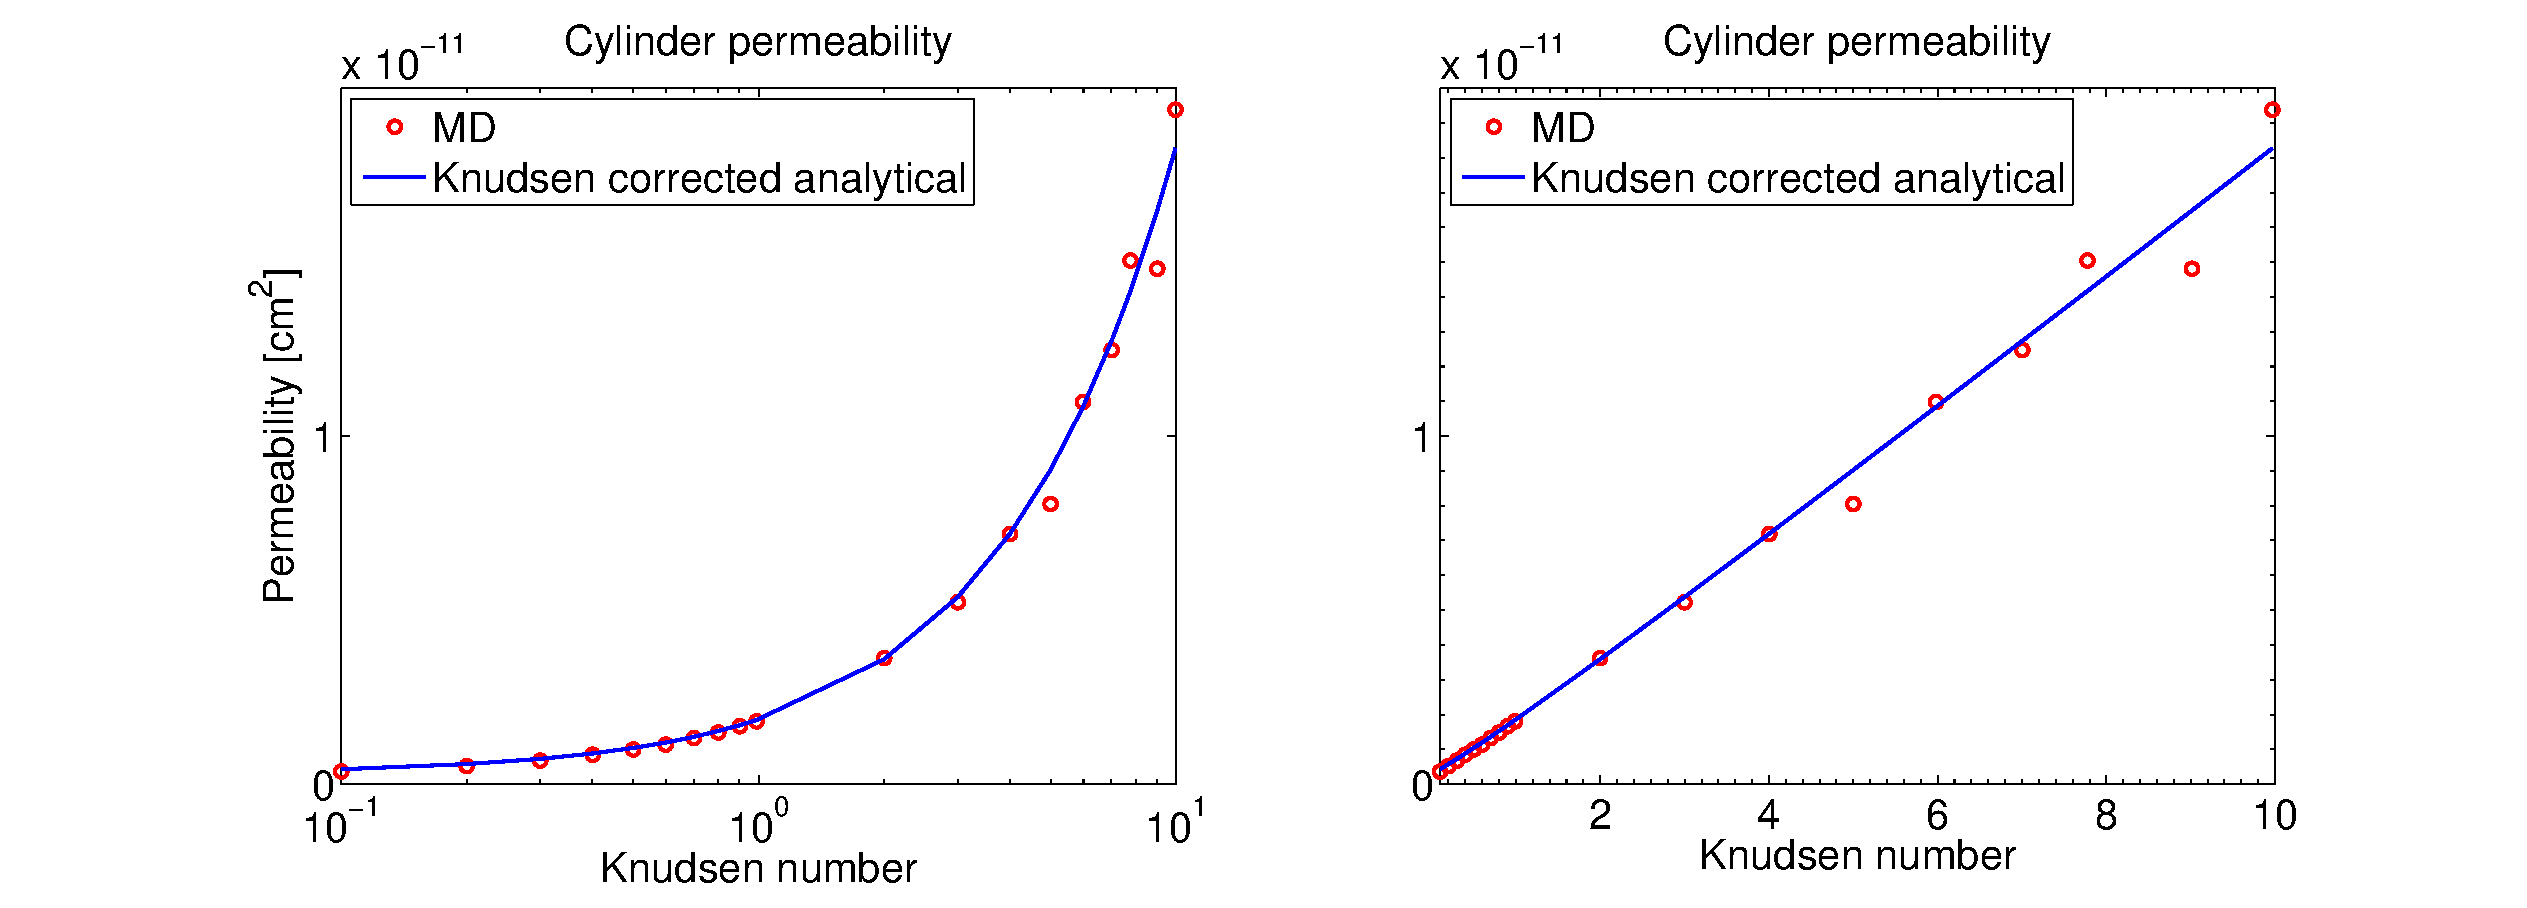
\includegraphics[width=1.0\textwidth, trim=0cm 0cm 0cm 0cm, clip]{MD/figures/permeability_cylinder.eps}
\end{center}
\caption{Permeabilities for Knudsen numbers in the range $0.1$ to $10.0$ in a cylinder with radius $r=$\unit{151}{\angstrom}. The left figure has a logarithmic $x-$axis to emphasize the good prediction in the lower Knudsen range. The right figure shows that the MD code produces results according to the Knudsen corrected permeability for a cylinder in equation \eqref{eq:cylinder_knudsen_corrected} in the entire range. The increased statistical noise is explained by that for large Knudsen numbers, the number of gas atoms is low.}
\label{fig:md_permeability}
\end{figure}
  \end{chapter}  
\end{part}

\begin{part}{Visualization}
  Whenever scientists perform an experiment in the lab or on a computer, they need to study the information outcome of the experiment. This could be the positions of some particles, the temperature of a gas or maybe the color of a fluid. Once we have this information, we need to represent it in a way that is useful for understanding the results. We often put numbers in a table or plot them as a graph. This is an extremely powerful ways to look at data and we can learn a lot by seeing how two or more variables are dependent of each other. It is convenient to introduce a general term, \textit{visualization}, which is just a visual representation of information (maybe not \textit{any} visual representation. Numbers in a table might be excluded.) One could say that a world map is a representation of the geometrical information describing how the continents are connected. The graph of some data is a relation between two or more variables. The output result from any computer simulation or experiment is information that can be visualized in some way.\\
There already exists a lot of software that can be used to visualize data in different ways. For particle simulations one can for example use \textit{VMD}\footnote{\url{http://www.ks.uiuc.edu/Research/vmd/}} or \textit{Ovito}\footnote{\url{http://www.ovito.org/}}. Both of these are great tools allowing us to visualize the time trajectories of atoms or particles. There are two drawbacks that have motivated the author to write a visualization tool from scratch.\\
In both VMD and Ovito, the way we navigate with the camera is inspired by other 3d software like 3ds Max, Maya and Blender where the camera is pointing towards a point whereas the mouse controls the position of the camera on the surface of a sphere centered in point. If we want to follow the movement of a single particle, this way of controlling the camera is inconvenient. We would like to control the camera in the way a space ship is controlled in a game, like in a first person shooter game. Here the mouse controls the direction the camera is looking and the camera position is controlled by the keyboard.\\
In addition, there are performance drawbacks with both programs where we have noticed that medium sized datasets (number of particles $\approx 1\e{6}$) give a frame rate that makes it very difficult to navigate around in the system. Also, the geometry of the DSMC code cannot be visualized in VMD or Ovito since these are particle visualizers only and the geometry is represented as a scalar field (the voxels from section \ref{sec:dsmc_complex_geometries}). To be able to solve these problems, we have implemented our own visualizer using OpenGL. In this chapter, we first give a brief introduction to OpenGL in section \ref{sec:opengl} explaining its basic ideas. We go through the concepts of vertices, primitives and how colors and textures are linearly interpolated from the values of the vertices. In section \ref{sec:opengl_coordinate_transformations} we discuss the three different coordinate spaces (model space, view space and projection space) that are used in the rendering. Vertex Buffer Objects are briefly explained in section \ref{sec:opengl_vbo} before we go through the sequence of shaders in the rendering pipeline in section \ref{sec:opengl_rendering_pipeline}. Note that this is not a complete introduction of OpenGL. Only the basic concepts that are required to understand how we have made the visualization tools are covered.
  \begin{chapter}{OpenGL}
    \label{chap:opengl}
    \section{What is OpenGL?}
\label{sec:opengl}
OpenGL (Open Graphics Library) is an open source graphics library providing an application programming interface (API) to communicate with a graphics processing unit (GPU) in order to get hardware-accelerated \textit{rendering}. Rendering is the process of generating an image from \textit{models} in an \textit{environment}. These models contain information about the geometry and associated textures. A model is typically represented by a set of points, triangles or some other set of \textit{primitives}. Before discussing the model, we should explain what a primitive is.
\subsection{Primitive}
In OpenGL, the primitive decides how to interpret a set of vertices. The same set of vertices may be interpreted, hence rendered, very different on the screen. Three points can be used to draw three single points, a triangle or a part of a rectangle among other different geometries. To illustrate this idea, in figure \ref{fig:opengl_primitives}, the four vertices $\{(0,0), (0,1), (1,1), (1,0)\}$ have been rendered with the primitives \textit{GL\_POINTS}, \textit{GL\_LINES}, \textit{GL\_TRIANGLES}, \textit{GL\_QUADS} and \textit{GL\_TRIANGLE\_STRIP}. The rendered objects are of course very different depending on the primitive. 
\begin{figure}[h]
\begin{center}
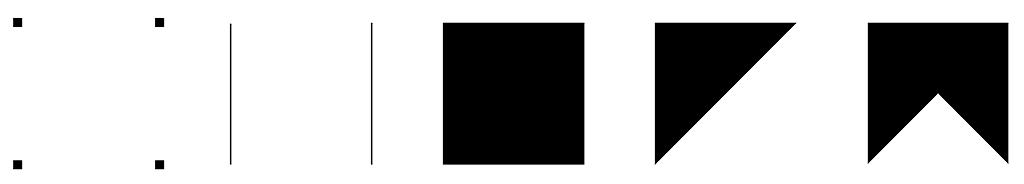
\includegraphics[width=\textwidth, trim=0cm 0cm 0cm 0cm, clip]{opengl/figures/primitives.png}
\end{center}
\caption{The vertices $\{(0,0), (0,1), (1,1), (1,0)\}$ have been rendered as the primitives (from left) \textit{GL\_POINTS}, \textit{GL\_LINES}, \textit{GL\_TRIANGLES}, \textit{GL\_QUADS} and \textit{GL\_TRIANGLE\_STRIP}. We see that the final rendered geometrical objects are quite different for the different primitives.}
\label{fig:opengl_primitives}
\end{figure}
When using for example the \textit{GL\_TRIANGLES}, OpenGL interprets groups of three vertices as one triangle. In the case of \textit{GL\_QUADS}, it will of course use groups of four vertices to define the renderable object. All of the primitives (except the \textit{GL\_POINTS}) form one or more two dimensional surfaces that are colored from either the interpolated values between the vertices or from a texture map which we now will explain.
\subsection{Color interpolation}
\label{sec:opengl_color_interpolation}
When creating a primitive consisting of $N$ vertices we can color each vertex $\vec r_i$ with an RGBA vector
\begin{align}
	\vec c_i = (r_i, g_i, b_i, \alpha_i)
\end{align}
where the components are the red, green, blue and alpha values for vertex $i$. The first three components defines the color whereas the last component is the transparency. In between the $N$ vertices, there are a lot of points that do not have a defined color value. OpenGL assigns colors to these inner points by \textit{linearly interpolating} the color values of the vertices. Any point $\vec p$ in a triangle defined by the three vertices $\vec p_a, \vec p_b$ and $\vec p_c$ can be uniquely specified by using \textit{barycentric coordinates} which is a set of three numbers $(a,b,c)$ in the range $[0,1]$, normalized so that $a+b+c=1$. \todo{cite the opengl specification} Once we have these coordinates, the point $\vec p$ in the global coordinate system (in which the vertices $\vec p_i$ are defined) is found as
\begin{align}
	\vec p = a\vec p_a + b\vec p_b + c\vec p_c.
\end{align}
The barycentric coordinates are found through
\begin{align}
	a = \frac{A(\vec p, \vec p_b, \vec p_c)}{A(\vec p_a, \vec p_b, \vec p_c)}, \qquad b = \frac{A(\vec p, \vec p_a, \vec p_c)}{A(\vec p_a, \vec p_b, \vec p_c)}, \qquad c = \frac{A(\vec p, \vec p_a, \vec p_b)}{A(\vec p_a, \vec p_b, \vec p_c)}.
\end{align}
We then use the barycentric coordinates as the weights in the linear interpolation so that the color at a point $\vec p$ is given as
\begin{align}
	\vec c(\vec p) = a\vec c_a + b\vec c_b + c\vec c_c,
\end{align}
where $\vec c(\vec p_i)$ is the color we gave the vertex at $\vec p_i$. In figure \ref{fig:opengl_color_interpolation} we see how the colors are interpolated from the three values at the triangle vertices.
\begin{figure}[h]
\begin{center}
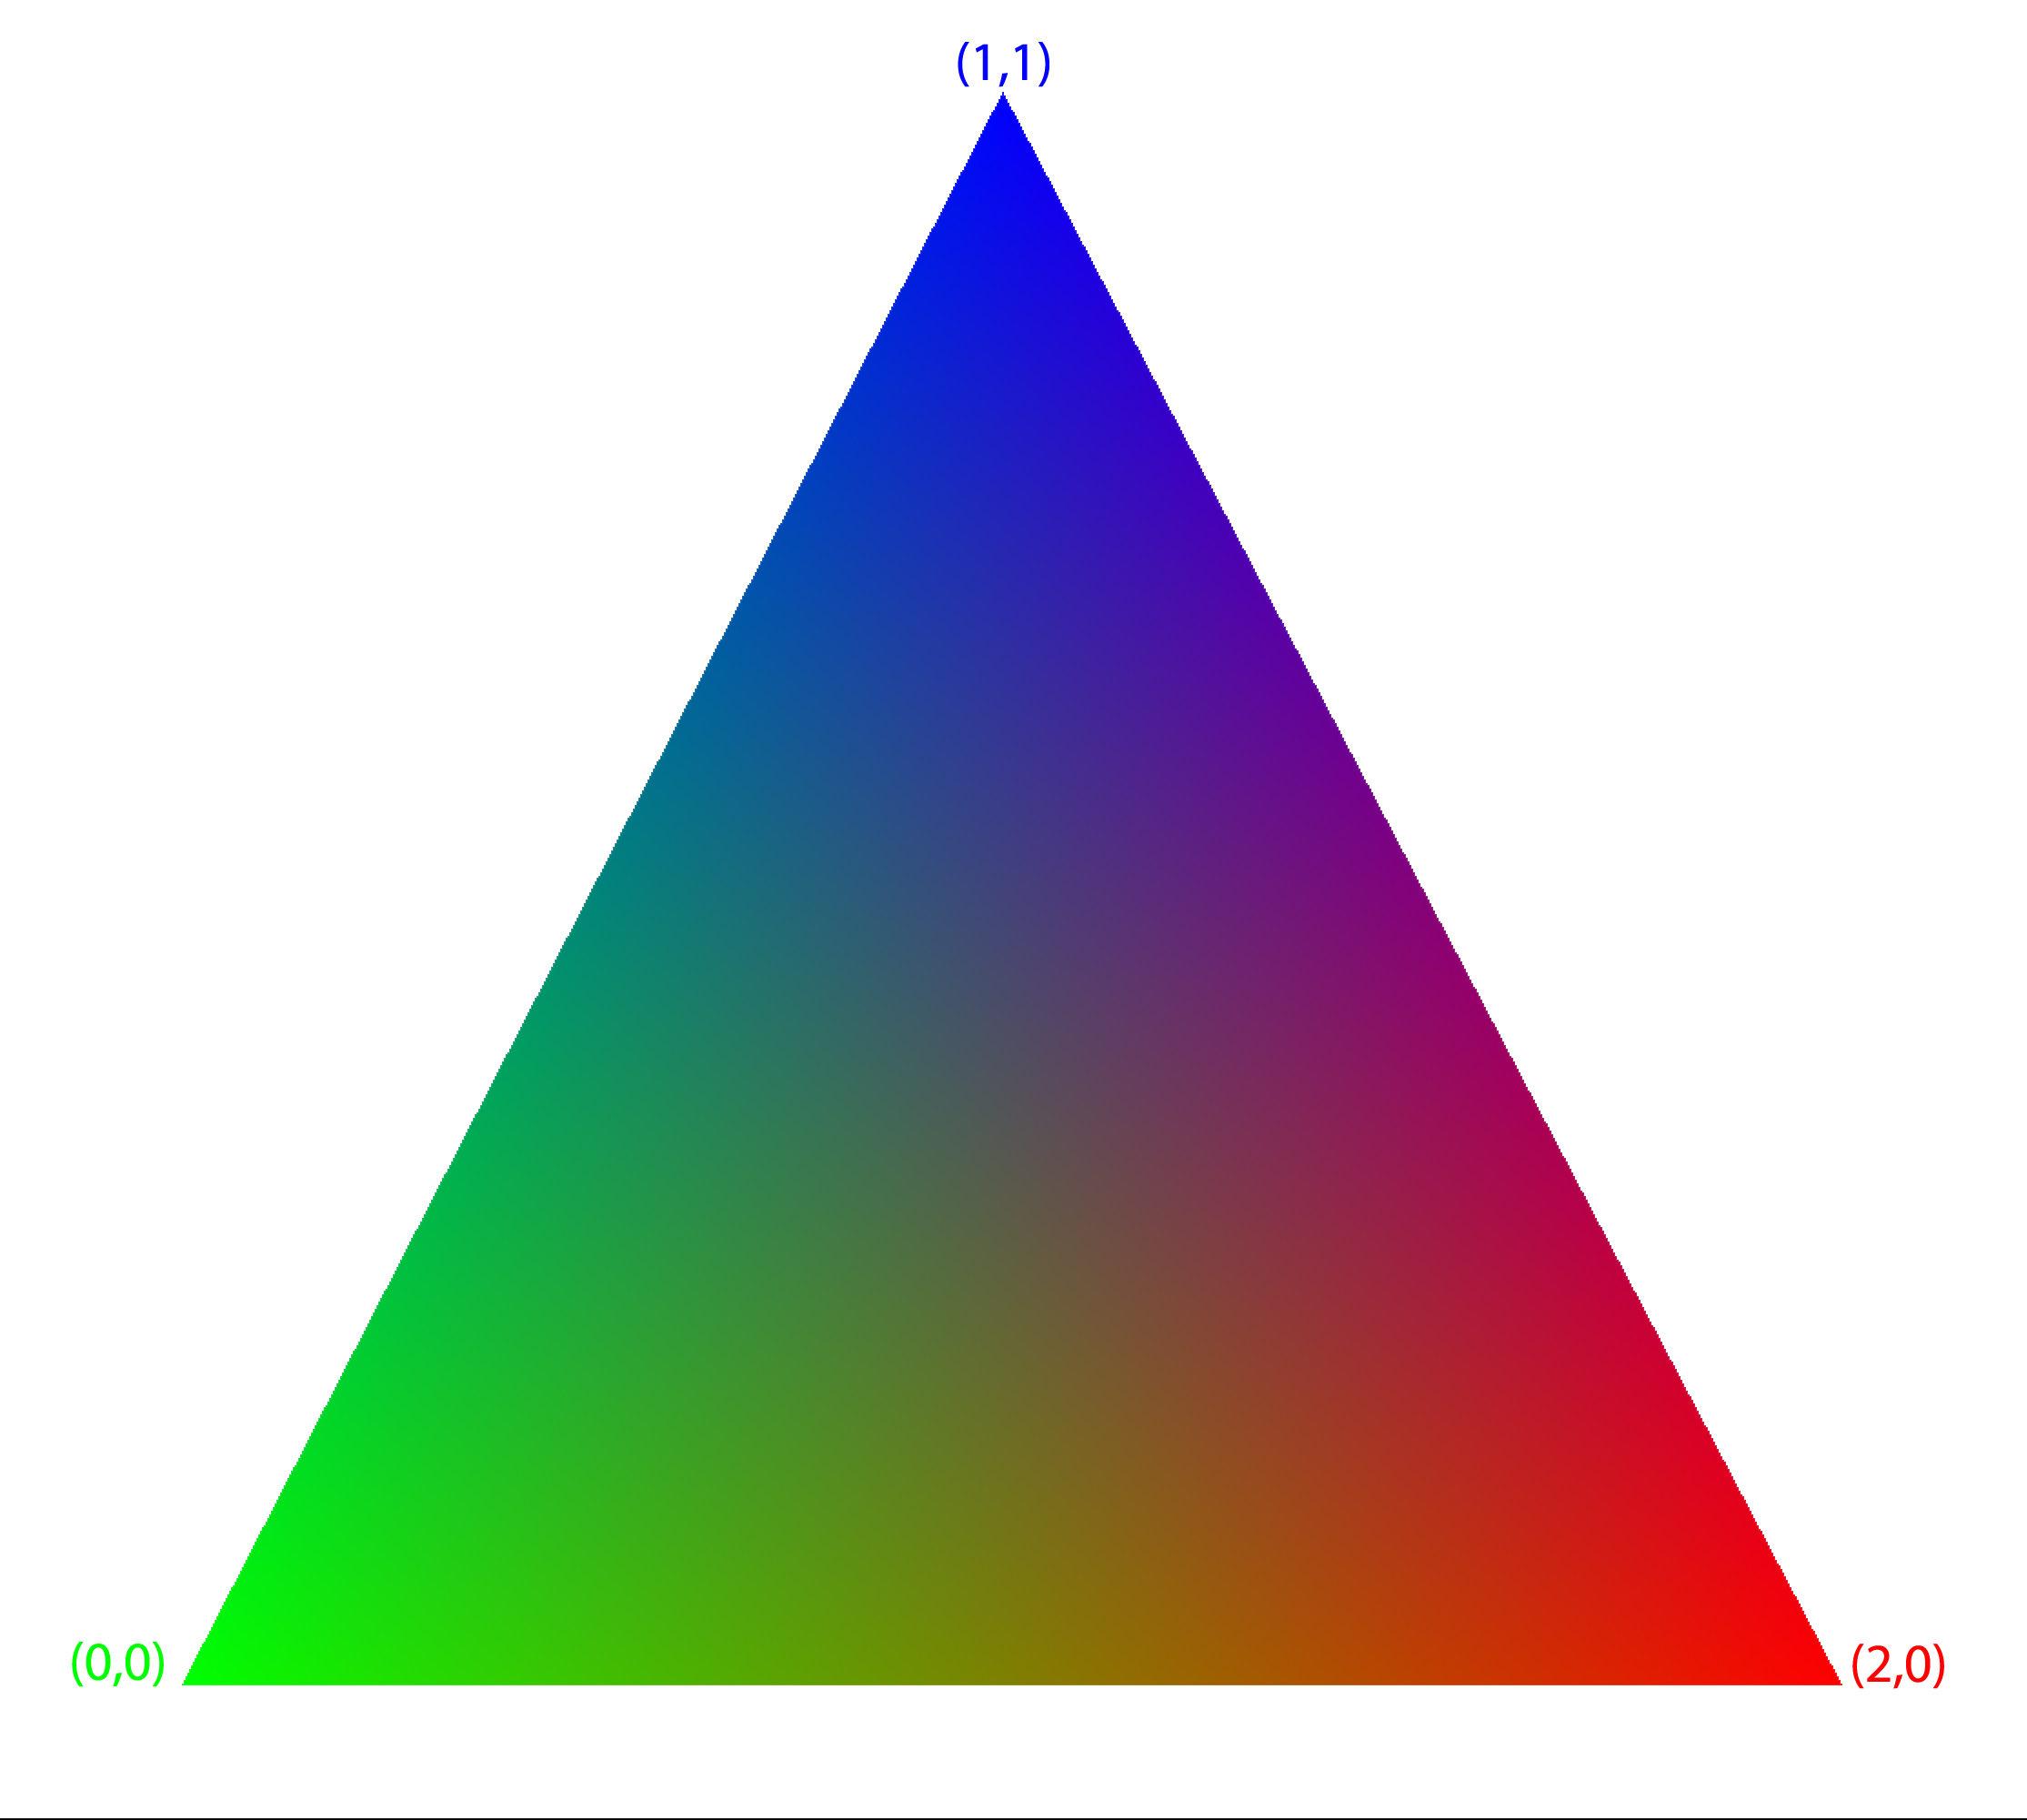
\includegraphics[width=\textwidth, trim=0cm 0cm 0cm 0cm, clip]{opengl/figures/color_interpolation.png}
\end{center}
\caption{The three vertices $\{(0,0), (1,1), (2,0)\}$ colored green, blue and red, forms a triangle where the inner points of the triangle is colored by the interpolation between the three vertices.}
\label{fig:opengl_color_interpolation}
\end{figure}
\subsection{Textures}
\label{sec:opengl_texture_interpolation}
Instead of using the colors specified per vertex, we can upload a texture (for example an image) to the graphics card so that the GPU can use that as the source of the color (this can be combined with the color values as we will see soon). The texture consists of $m\times n$ pixels where each pixel has a color $\vec c_t$. Each vertex $i$ of the triangle is assigned a \textit{local texture coordinate} 
\begin{align}
	\vec t_i = (t_x, t_y),
\end{align}
where $t_x, t_y \in [0,1]$. This gives the mapping to the \textit{global texture coordinates} (the actual pixel coordinates) $\vec t^* = (t_x^*, t_y^*)$ where 
\begin{align}
	\nonumber
	t_x^* &= m\cdot t_x\\
	t_y^* &= n\cdot t_y,
\end{align}
where we have added the asterisk on the global coordinates since we will mostly use the local ones. Since each pixel $\vec t$ (remember these are the local coordinates) in the texture has a color value $\vec c_t(\vec t)$, we can find the color $\vec c(\vec p)$ of a point $\vec p$ within the triangle by interpolating the local texture coordinates as we interpolated the colors. Remember that the point $\vec p$ has barycentric coordinates $(a,b,c)$, so the local texture coordinates $\vec t$ are found by
\begin{align}
	\vec t(\vec p) =  a\vec t_a + b\vec t_b + c\vec t_c,
\end{align}
where $\vec t_i$ is the local texture coordinate assigned to vertex $i$. The color of this point $\vec p$ is then simply
\begin{align}
	\vec c(\vec p) = \vec c_t[\vec t(\vec p)].
\end{align}
In figure \ref{fig:opengl_texture_interpolation} we have illustrated how the texture interpolation works. In the left figure, the texture is mapped with  texture coordinates corresponding to the coordinates of the triangle vertices. In the figure to the right we have a skewed mapping making the image look skewed.
\begin{figure}[h]
\begin{center}
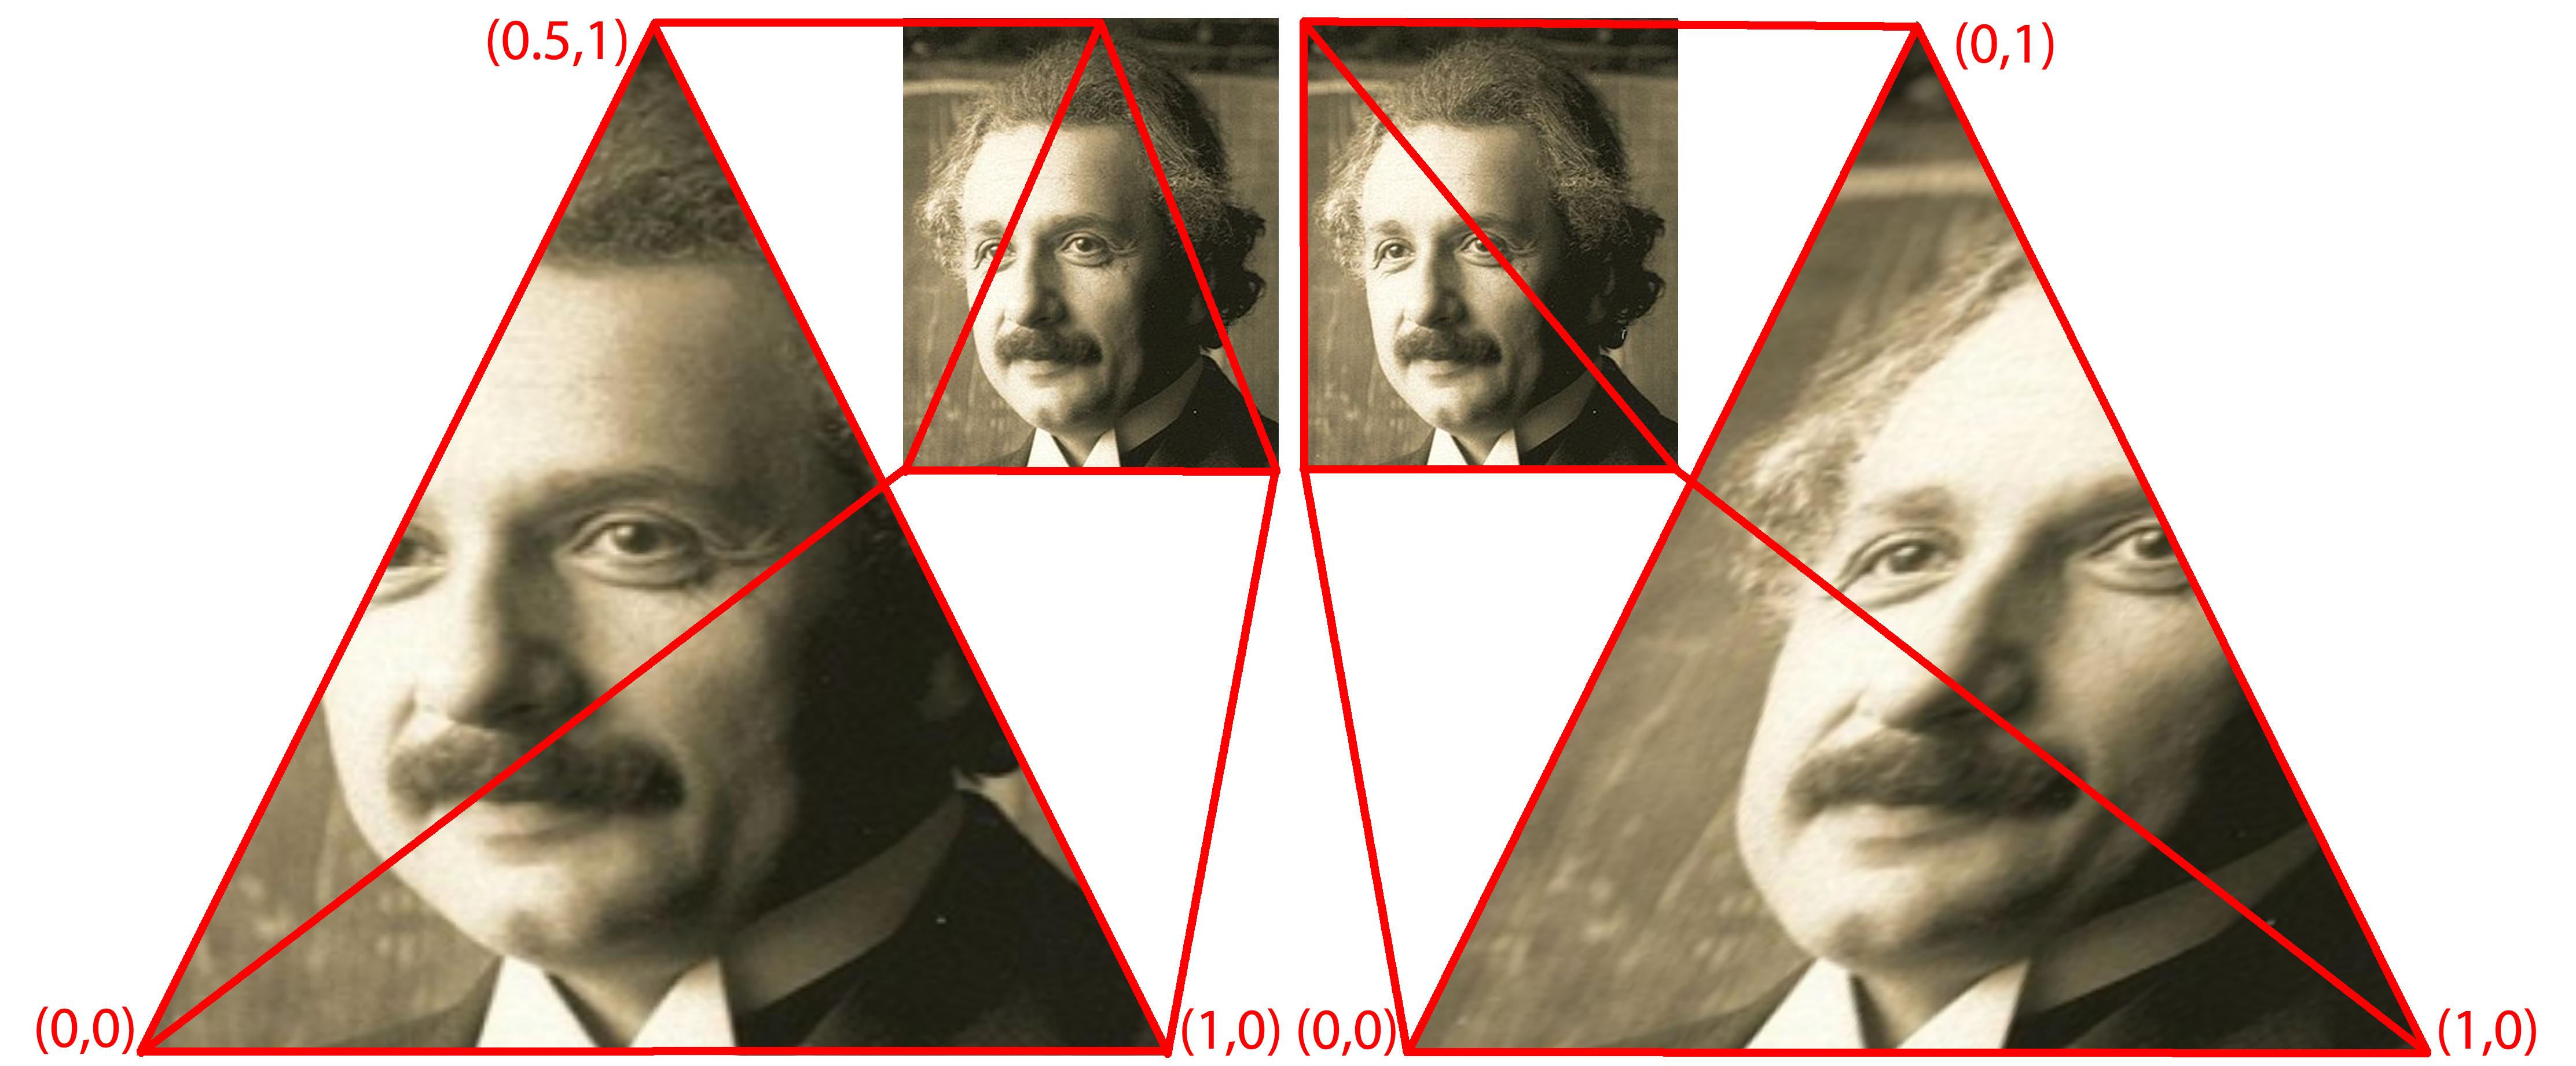
\includegraphics[width=\textwidth, trim=0cm 0cm 0cm 0cm, clip]{opengl/figures/texture_interpolation.png}
\end{center}
\caption{Showing how texture interpolation works. Left: the three vertices $\{(0,0), (1,1), (2,0)\}$ are assigned the local texture coordinates $\{(0,0), (0.5,1), (1,0)\}$ where we see how the texture are transformed onto the triangle . Right: the three vertices $\{(0,0), (1,1), (2,0)\}$ are assigned the local texture coordinates $\{(0,0), (0,1), (1,0)\}$ where we see that the texture on the triangle is skewed because of the transformation. Note that the coordinates in the figure at the vertices are the texture coordinates, not the coordinates of the vertices.}
\label{fig:opengl_texture_interpolation}
\end{figure}
We can of course combine both these methods (colors and textures) by applying both a texture coordinate \textit{and} a color value to each vertex. OpenGL will then render an image where the rendered color $\vec C$ becomes
\begin{align}
	\label{eq:opengl_combining_colors_textures}
	\vec C(\vec p) = \vec c_t[\vec t(\vec p)] \odot \vec c(\vec p),
\end{align}
where $\odot$ is the element-wise multiplication operator defined as
\begin{align}
	(\vec a \odot \vec b)_i = a_i\cdot b_i,
\end{align}
where $\vec a,\vec b \in \mathbb{R}^N$ and $d_i$ is the $i$'th component of some vector $\vec d$. In figure \ref{fig:color_and_texture} we have combined both the color and the texture giving a triangle with the same image of Albert Einstein colored in the same way as the triangle in figure \ref{fig:opengl_color_interpolation}.
\begin{figure}[h]
\begin{center}
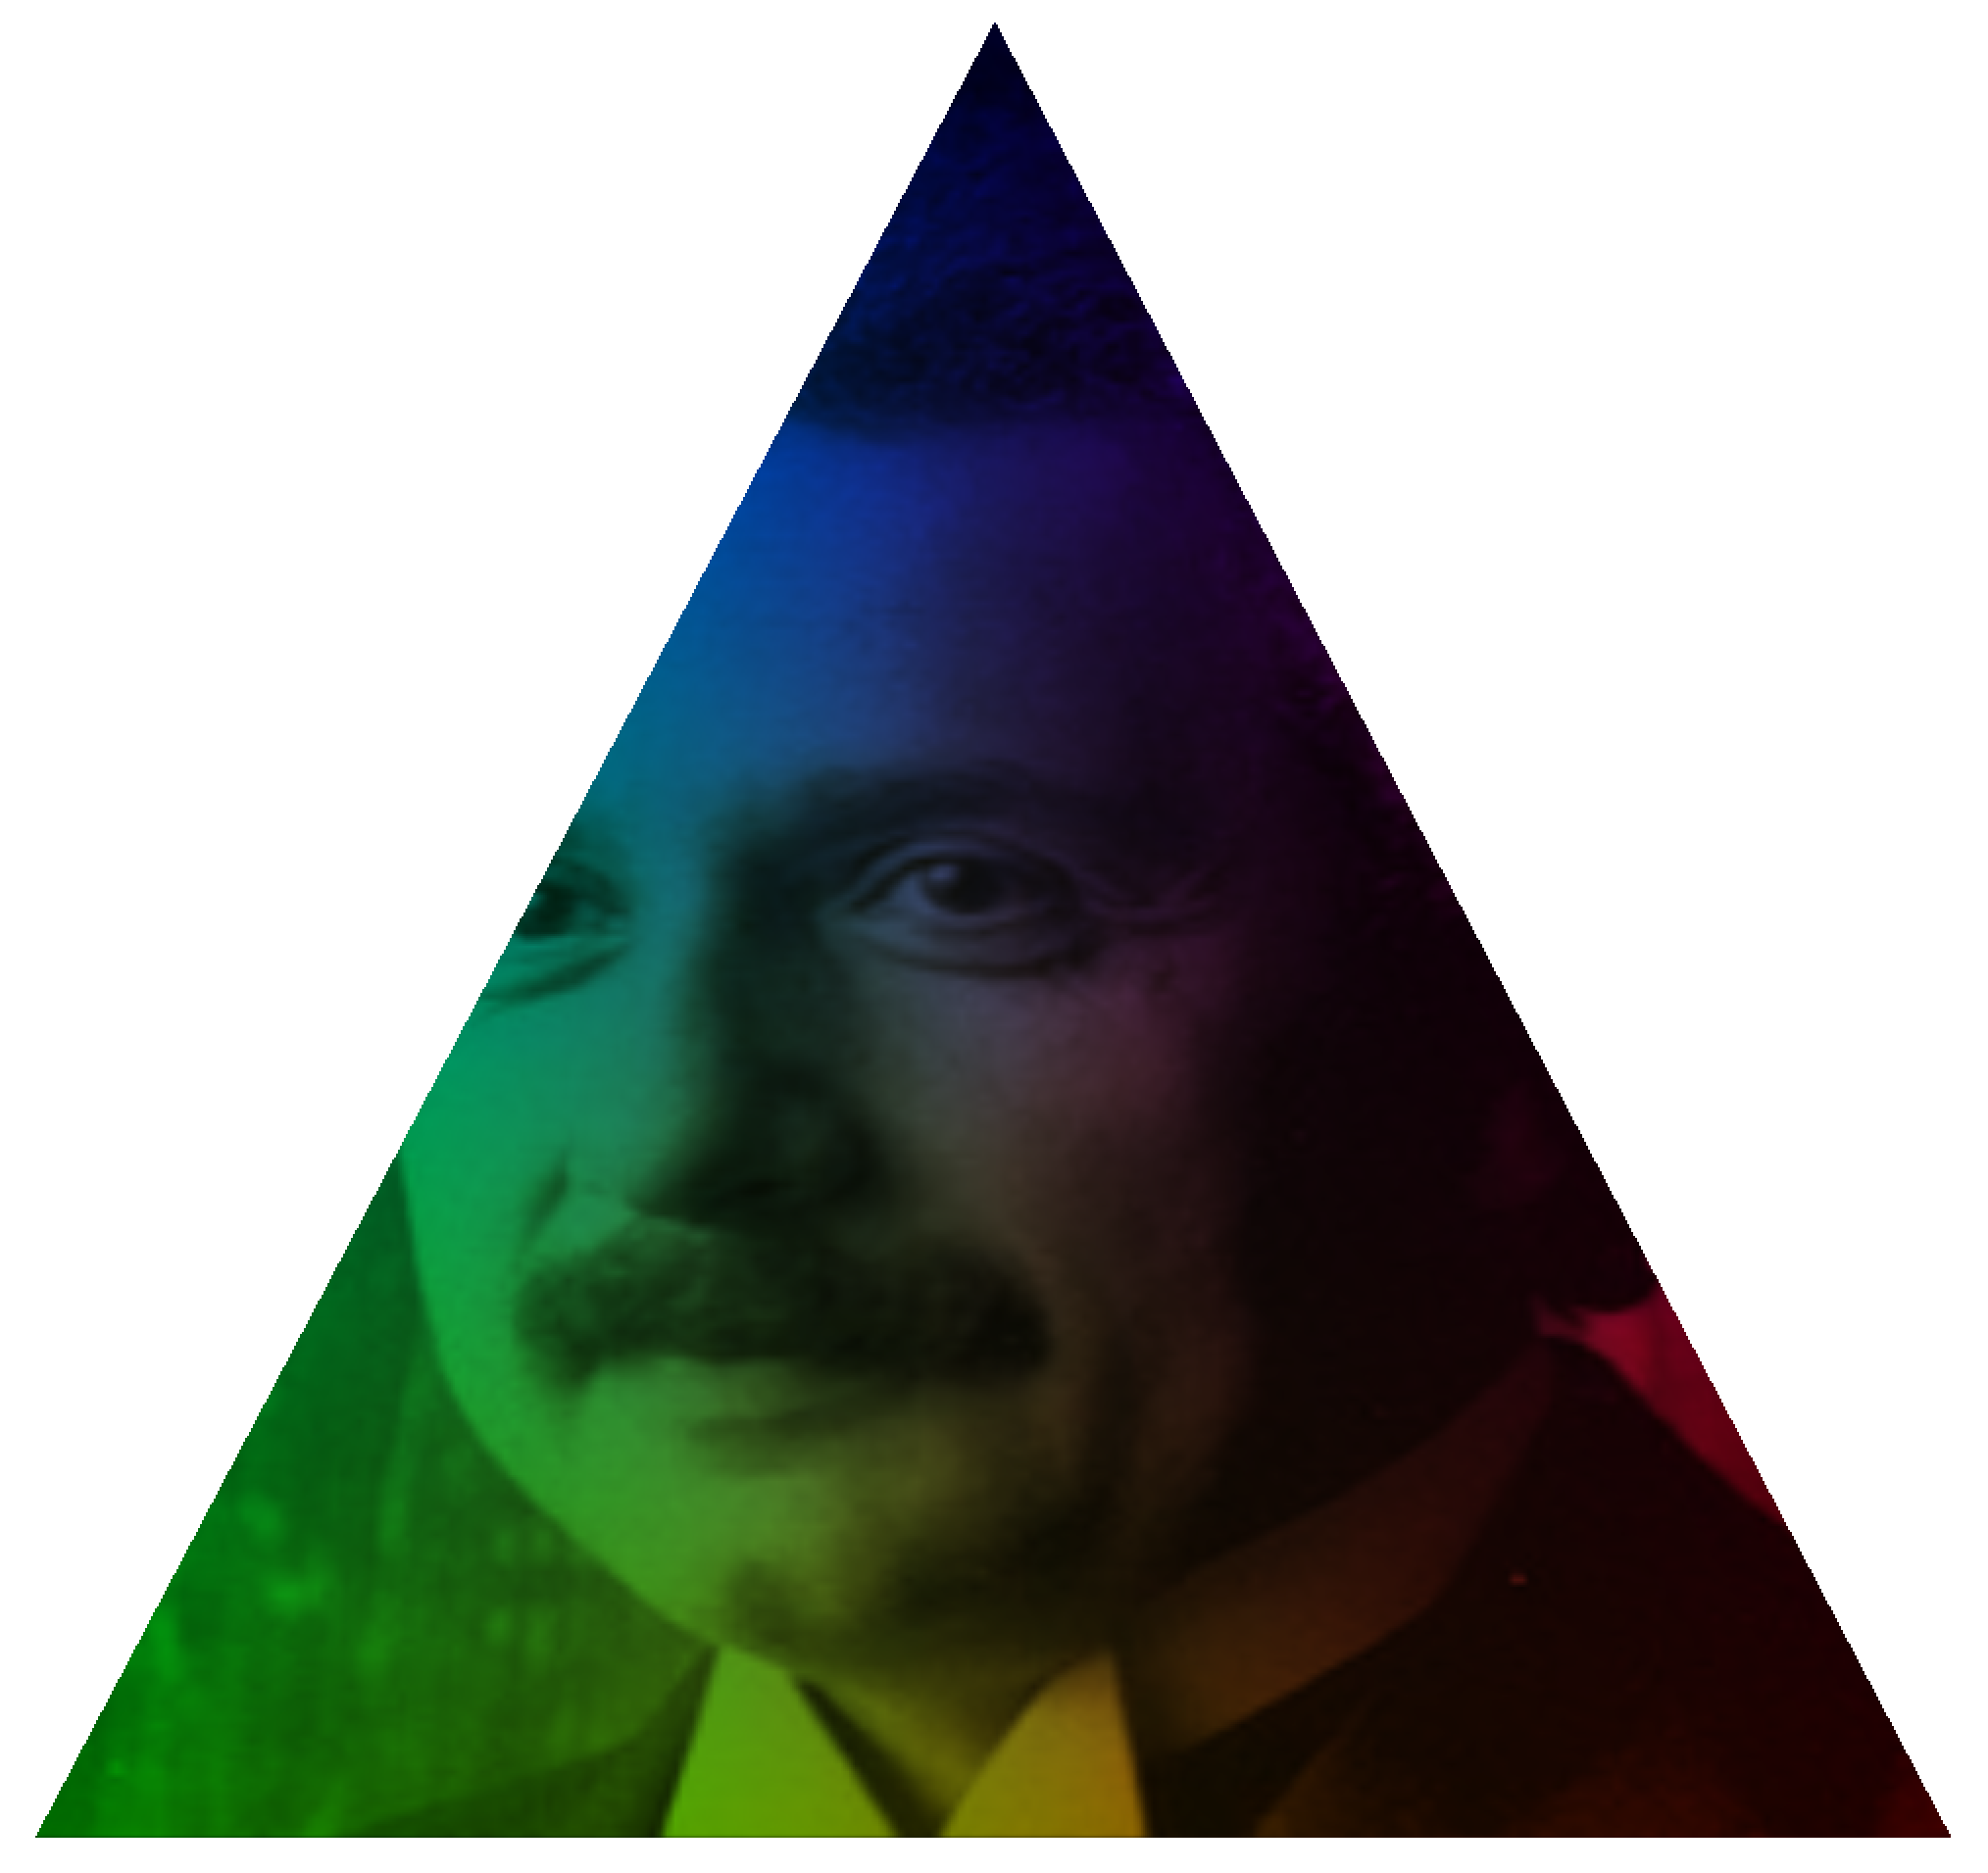
\includegraphics[width=\textwidth, trim=0cm 0cm 0cm 0cm, clip]{opengl/figures/color_and_texture.png}
\end{center}
\caption{We can combine both colors and textures to color points within a triangle according to equation \eqref{eq:opengl_combining_colors_textures}. Here we have used the same colors as in figure \ref{fig:opengl_color_interpolation} and the texture of Albert Einstein in figure \ref{fig:opengl_texture_interpolation}.}
\label{fig:color_and_texture}
\end{figure}
\subsection{Model}
\label{sec:opengl_model}
A model of an object contains all the information fully defining how a geometric object looks like without any effects from the environment such as light or distortions from a water surface. The model is fully described by a set $\mathcal{M}$ containing primitive objects $\mathcal{P}$, each having 
\begin{itemize}
	\item a vertex array,
	\item the primitive type,
	\item a color array,
	\item a texture id,
	\item a local texture coordinate array, and
	\item a normal vector array.
\end{itemize}
We have discussed the array of vertices, the primitive, the color and texture coordinate arrays (remember, one color and/or one texture coordinate per vertex). We also need the id (which is just an int variable) allowing us to tell the GPU which texture it should apply to this primitive object. In addition, we can assign a \textit{normal vector} to each vertex which can be used to create realistic lighting and other effects. It's time for an example of a model.\\
Say we want a model of a die. A die is a cube with six faces. The model $\mathcal M$ would then contain six primitive objects $\mathcal P_i$, each having an array of four vertices. The primitive type would be \textit{GL\_QUADS} where the color of course could be your favorite. We need to upload six textures (one face has one dot, another face has two dots etc) which gives us six different texture id's. The local texture coordinate array is simply the four corners of the unit square whereas the normal vectors should point outwards from the cube. In figure \ref{fig:opengl_die} we haved used this technique to draw a red die.
\begin{figure}[h]
\begin{center}
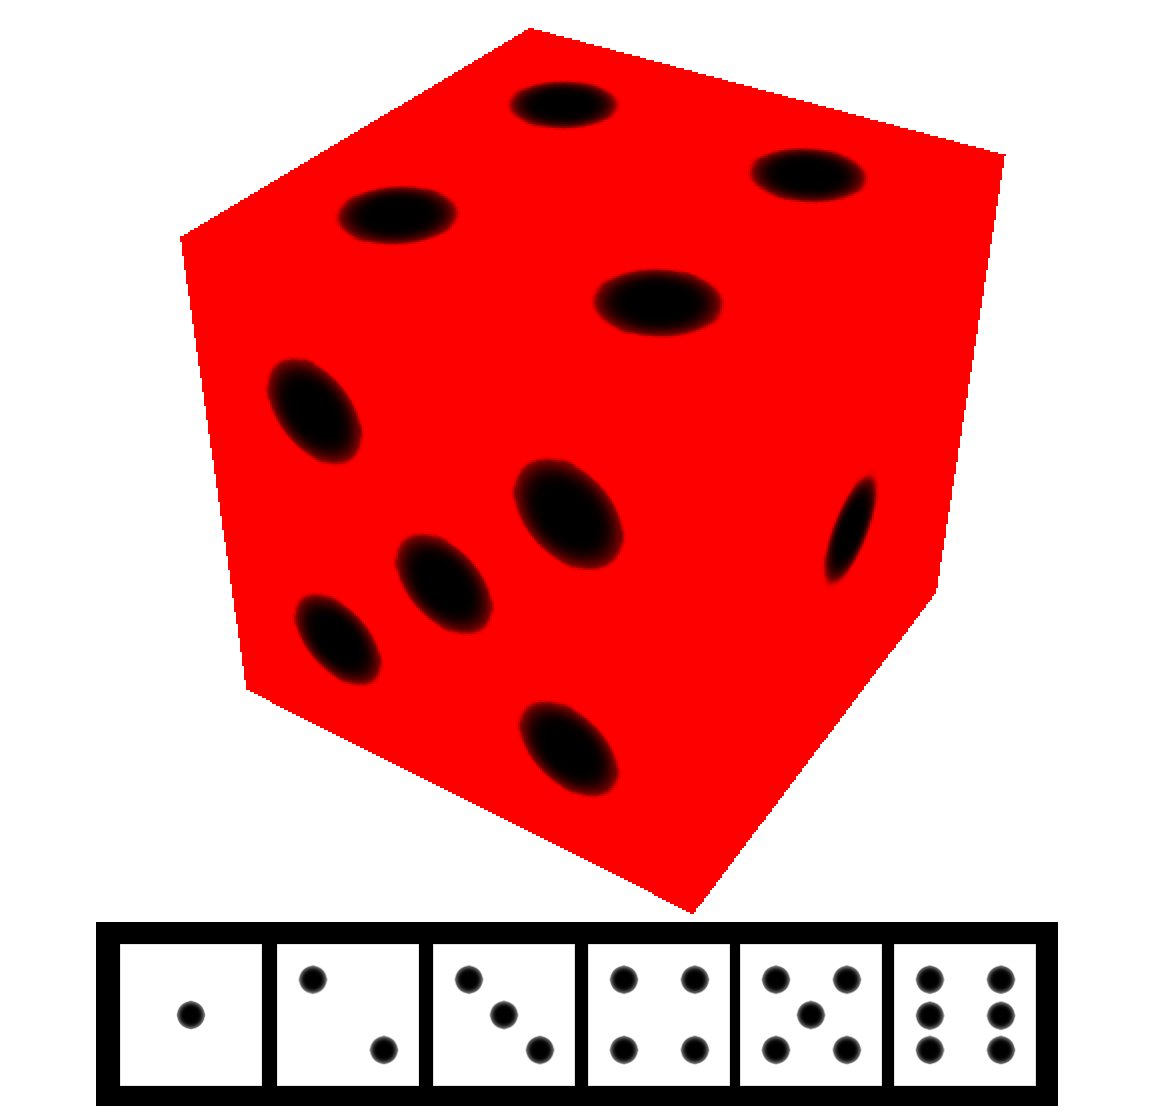
\includegraphics[width=\textwidth, trim=0cm 0cm 0cm 0cm, clip]{opengl/figures/die.png}
\end{center}
\caption{Drawing a die using the technique described in subsection \ref{sec:opengl_model}. The color was chosen to be red whereas each of the six faces were assigned one of the textures in the black box.}
\label{fig:opengl_die}
\end{figure}
    \section{Vertex Buffer Objects}
\label{sec:opengl_vbo}
A Vertex Buffer Object (VBO) is a feature in OpenGL that allows the user to upload an array of vertices to the graphics card which can be used for fast rendering. This could for example be a set of positions, colors or normal vectors. Once this data is uploaded to the GPU, we can render the model described by the VBO in very few function calls. First, we ask the GPU to give us a buffer identifier (which is just an int) that we will use when we work with the VBO (uploading new data or using the data). Then we tell the GPU to allocate enough memory to store our vertices before we copy the data from the main memory to the graphics card.
    \section{Rendering pipeline}
\label{sec:opengl_rendering_pipeline}
\todo{Explain that the shaders are run in massive parallel}
Now that we know what a VBO is, we are ready to render the objects described by a set of VBOs on the screen. First we activate the data we want to render by telling the graphics card what VBO identifier represents the positions, colors, normal vectors and texture coordinates. Then we ask the GPU to render the activated data as the primitive the vertices represent (we know if the vertices should be rendered as triangles, quads or lines). The data then goes through what's called the \textit{rendering pipeline} which is a set of programs (they are called shaders) on the GPU that processes the data, going from the vertices to the actual colors on each of the pixels on your monitor. In this section we discuss the different steps in the rendering pipeline that are relevant to describe the visualization tools developed by the author. In figure \ref{fig:opengl_rendering_pipeline} we have illustrated the rendering pipeline containig the stages that we have used. 
\begin{figure}[h]
\begin{center}
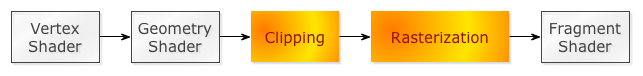
\includegraphics[width=\textwidth, trim=0cm 0cm 0cm 0cm, clip]{opengl/figures/pipeline.png}
\end{center}
\caption{Diagram of the OpenGL rendering pipeline. The gray boxes are shader steps (the shader programs can be written by the user). Each vertex is processed in the vertex shader before it is sent to the geometry shader that can create zero or more vertices based on the input vertex. Each vertex is then analyzed in the clipping program that removes vertices that cannot be rendered. The rasterization program creates a two dimensional image of every triangle so that the fragment shader can merge everything to color values per pixel on the screen. Not that the full pipeline contains more steps, but these are the relevant stages for understanding what our visualization tool does.}
\label{fig:opengl_rendering_pipeline}
\end{figure}
\subsection{Uniforms, ins and outs}
\label{sec:opengl_uniforms}
\subsection{Vertex shader}
The vertex shader is executed once per vertex in the input VBOs. It specifies which input vertex that is to be interpreted as the position, color, normal vector and/or texture coordinate if they are specified. The input position vertex is usually in the model space which are local coordinates for this specific object. A typical vertex shader applies the Model View Projection matrix on the vertex, transforming it from the model space to the projection space which often is assumed in the later pipeline stages. The latter may be done on the geometry shader instead if a three dimensional object is created at that stage.
\subsection{Geometry shader}
Each vertex from the vertex shader is a part of a primitive (such as \textit{GL\_POINTS} or \textit{GL\_TRIANGLES}). A geometry shader takes a primitive (i.e. a set of vertices, each processed by the vertex shader) as input and outputs zero or more primitives that may be of another type than the input primitive. A typical use is to describe a geometrical object (this could be a sphere or a tube) on the geometry shader so that the input primitive is just one single vertex; the position. This significantly reduces the memory and bandwidth usage on the GPU which usually gives great performance improvements.\\
The geometry shader can also be run in \textit{instancing mode} which means that the shader program is run a given number of time per vertex with an invocation id given. If a particle system obeys periodic boundary conditions, we can for example use the geometry shader instancing to add 26 periodic copies of the system making the system look larger than it is. 
\subsection{Clipping}
After the geometry shader has decided which primitives we want rendered, some of the vertices may not be visible on the screen. They can be behind the camera, too far to the right or in some way outside the camera view. When we in the final stages (the fragment shader) are going to decide colors on every pixels, we don't need to compute primitives that does not contribute to the final image. This is called clipping and is a very simple process to perform in the projection space. All vertices outside the clip volume (the volume that will be rendered) will be discarded and not computed at the rasterization stage.
\subsection{Rasterization}
The rasterization program will for each primitive determine which pixels that are a part of the primitive. Each active pixel will have interpolated colors and texture coordinates as described in subsection \ref{sec:opengl_texture_interpolation} before we reach the fragment shader, the final stage in the rendering pipeline.
\subsection{Fragment shader}
The fragment shader is executed one time \textit{per pixel} for each of the primitives that contributes to that pixel. 
  \end{chapter}
  
  \begin{chapter}{Advanced particle visualizer}
    \label{chap:particle_visualizer}
    With our newly acquired knowledge about OpenGL and learned how we can use the API to render objects on the screen, we have everything we need to develop our own visualization tools that can handle datasets from both MD and DSMC. As we now should be well aware of, the state of a system with $N$ particles is described by the $3N$ particle positions and the $3N$ velocity components. If we save this information every timestep of a simulation, we can use it to render a time series, an animation of the trajectories of all the particles. We will render the particles as spheres, but areg oing to cheat a bit. An actual sphere rendered in OpenGL would need to be composed of many triangles forming the spherical shape. To be able to render a smooth sphere, we would need more than 100 triangles \textit{per sphere} as we will see in section \ref{sec:vis_billboards}. We will apply a trick used in computer games for years. Instead of rendering spheres, we use something called \textit{billboards}, which is a rectangle with an \textit{image} (a texture) of a sphere, always pointing towards the camera. In section \ref{sec:vis_billboards}, we explain how we effectively can create and render billboards with the goemetry shader on the GPU. If the particle system has periodic symmetry (both MD and DSMC use periodic boundary conditions), we can also use the geometry shader to render copies of the system, making the illusion that the system is larger than it really is.\\
When we visualize a dataset from a DSMC simulation, we should, in addition to the particle positions, render the surface geometry (which, as we remember from section \ref{sec:dsmc_complex_geometries}, is a voxelized scalar field). We will then be able to see the surface the particles collide with which will make it easier to understand their behavior. In section \ref{sec:marching_cubes}, we discuss the so-called \textit{marching cubes} algorithm, which allows us to create a set of renderable triangles from the isosurface of a scalar field (the points where the scalar field values intersect some value).\\
We conclude the chapter by explaining how such a program was extended to render 3D images on an Oculus Rift\footnote{The Oculus Rift is a virtual reality headset displaying a stereoscopic rendering giving realistic 3D effects. The Rift has head tracking, allowing the user to tilt and rotate the head so he/she can look around in the virtual world.} in section \ref{sec:oculus_rift}. The same rendering technique was used to visualize the particles in 3D on a 3D TV.
    \section{Billboards}
\label{sec:vis_billboards}
We could in principle create a spherical shape by connecting triangles and/or other primitives as illustrated in figure \ref{fig:visualization_glut_spheres}. The figure contains two spheres with different numbers of primitives. We need a substantial number of primitives to get a shape that looks like a sphere (200 in the left sphere in the figure), but we can cheat a bit, by instead rendering something that \textit{looks} like a sphere
\begin{figure}[h]
\begin{center}
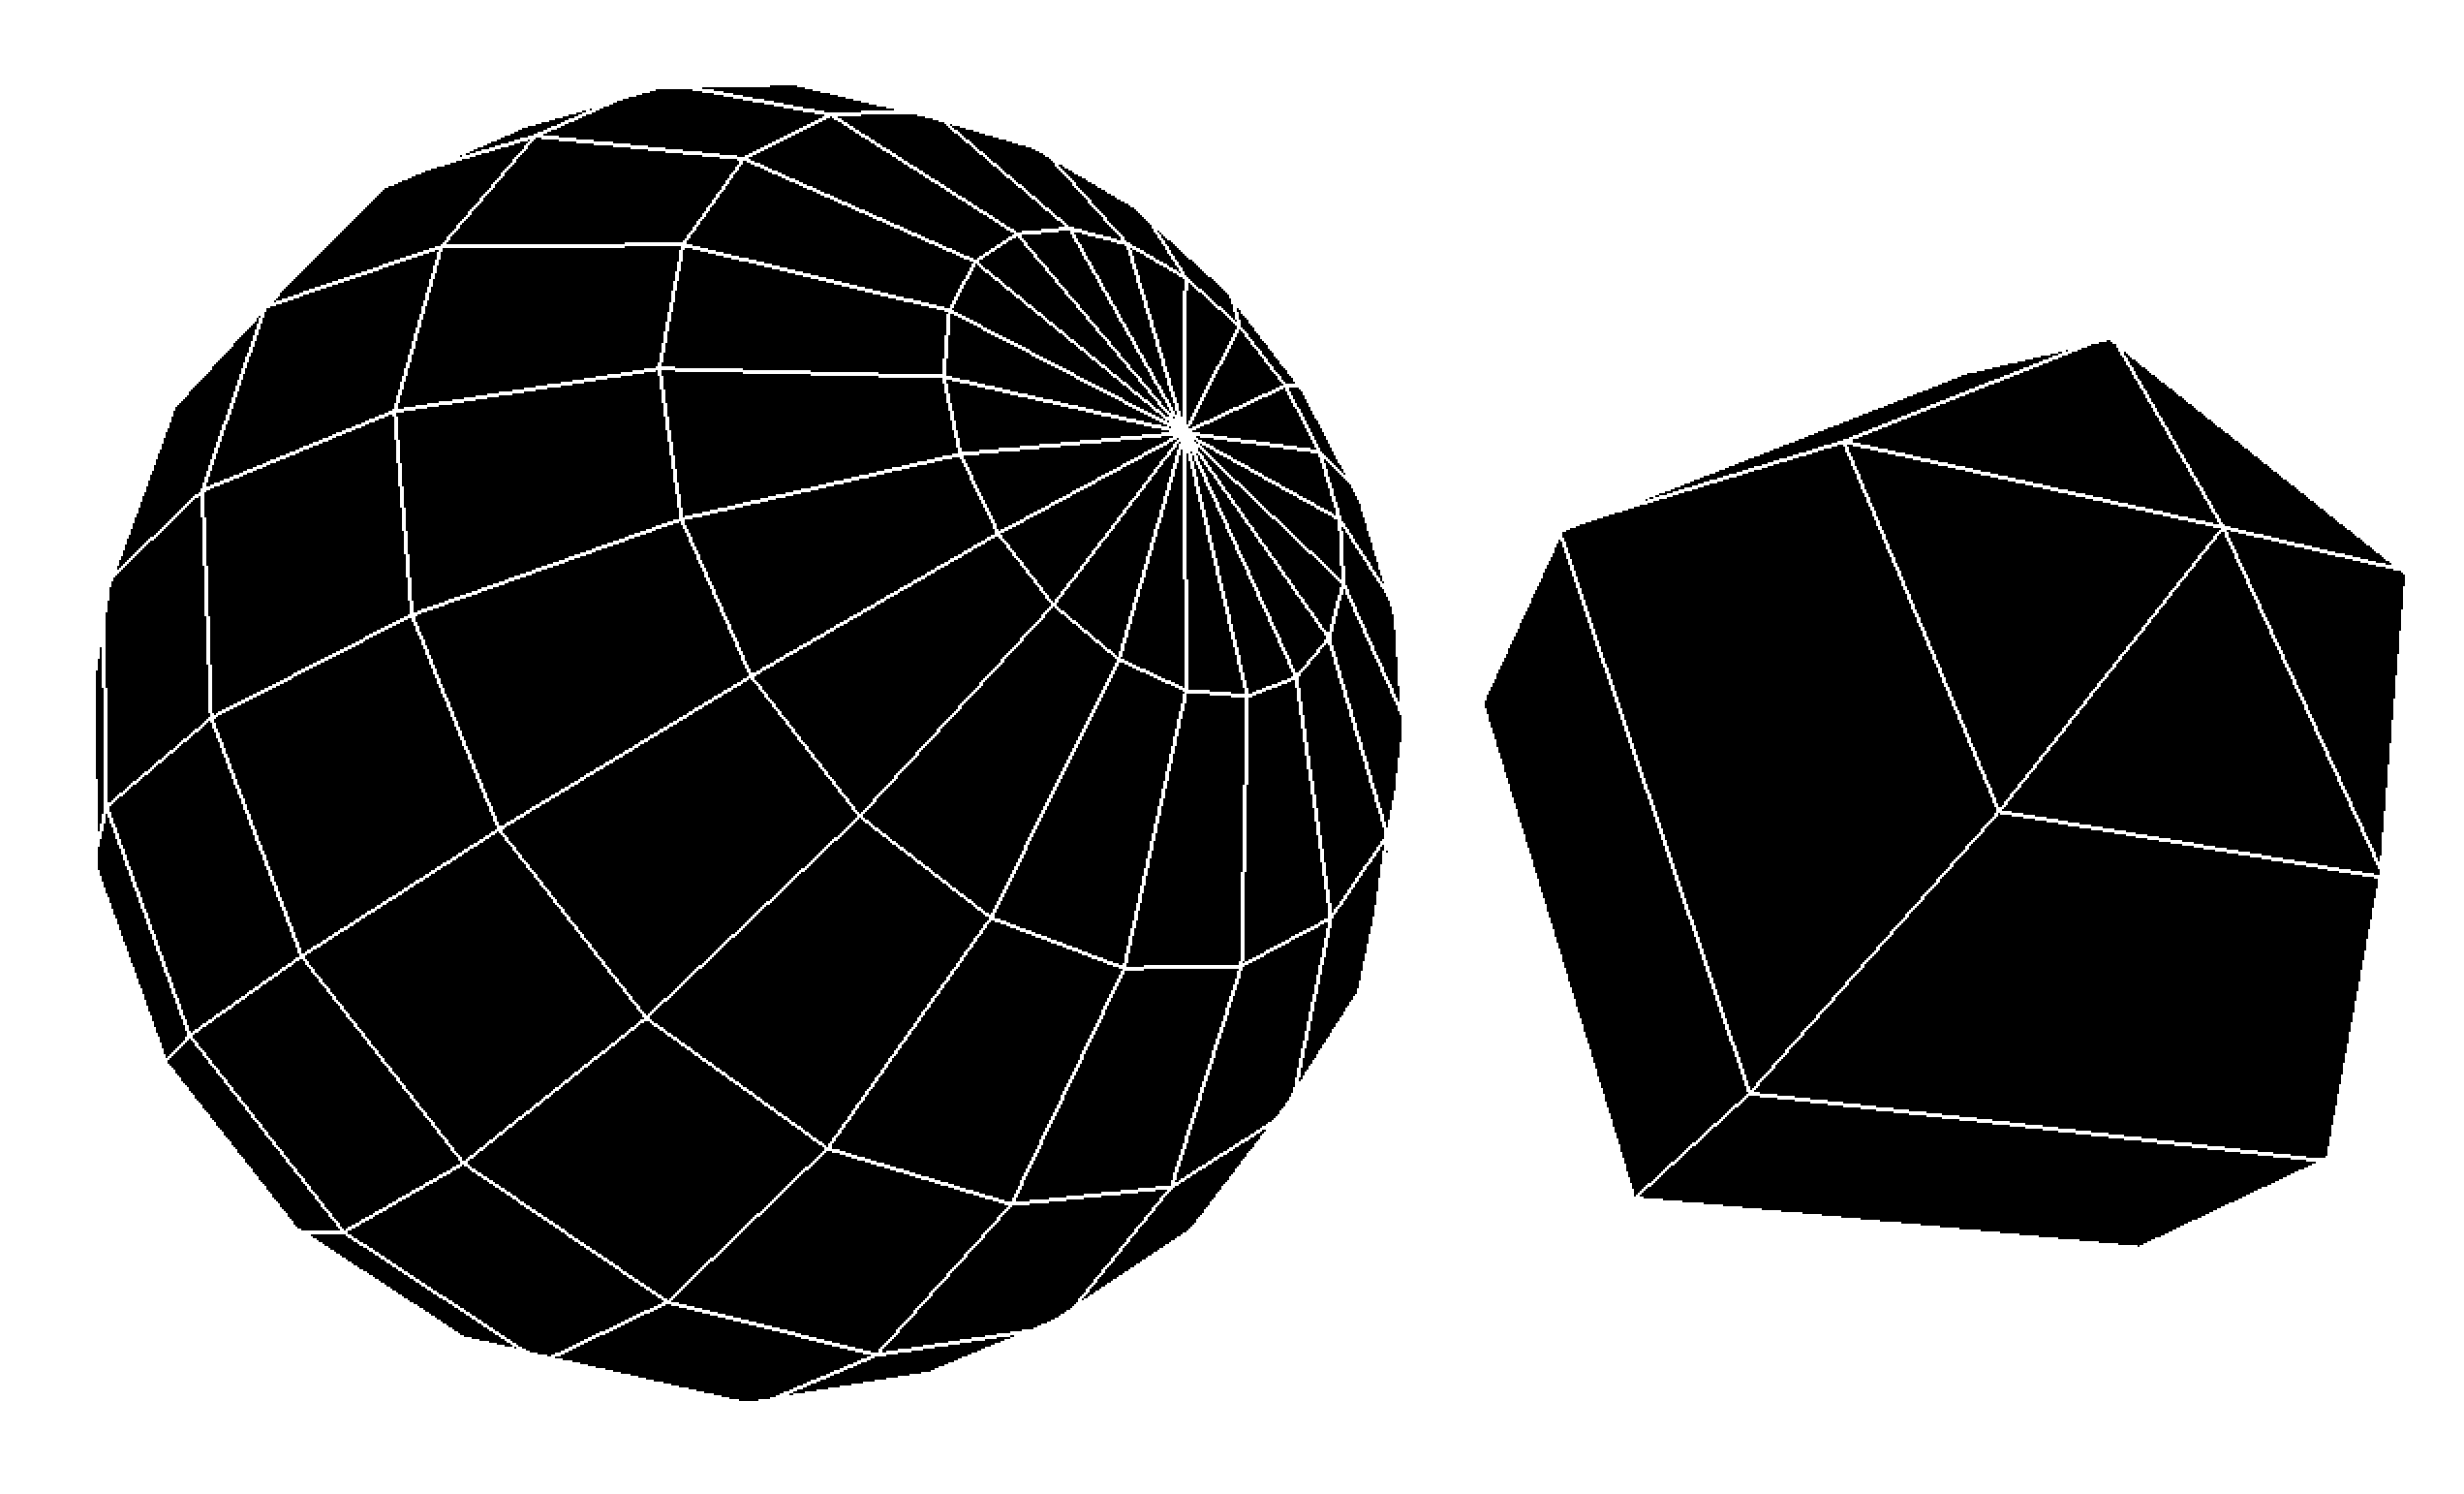
\includegraphics[width=0.8\textwidth, trim=0cm 0cm 0cm 0cm, clip]{visualization/figures/glut_spheres.png}
\end{center}
\caption{A sphere can be created by connecting triangles and/or other primitives. The sphere to the left is made of 200 primitives whereas the one to the right is made of 25 primitives. It is clear that we need a certain number, more than 25, of primitives before we are convinced that the object should represent a sphere.}
\label{fig:visualization_glut_spheres}
\end{figure}
A billboard is, as the name suggests, a rectangle filled with a texture, always pointing towards the camera. The texture is going to be a circle (a sphere does indeed look like a circle when rendered on the screen anyway). It is quite easy to render such a rectangle with OpenGL, we already have a primitive called \textit{GL\_QUADS} which is exactly what we need. The only thing we need to do is provide four vertices, the corners in the rectangle, and give each vertex a texture coordinate. The four vertices $\vec v_i$ can be calculated from one single vertex $\vec r$, the particle position, by
\begin{align}
	\label{eq:vis_vertices_billboard}
	\vec v_1 &= \vec r + (-\Delta x, -\Delta y)\\
	\nonumber
	\vec v_2 &= \vec r + (-\Delta x, \Delta y)\\
	\nonumber
	\vec v_3 &= \vec r + (\Delta x, \Delta y)\\
	\nonumber
	\vec v_4 &= \vec r + (\Delta x, -\Delta y),
\end{align}
where ($L_x = 2\Delta x, L_y = 2\Delta y$) is the size of the billboard, see figure \ref{fig:visualization_billboard_vertices}.
\begin{figure}[h]
\begin{center}
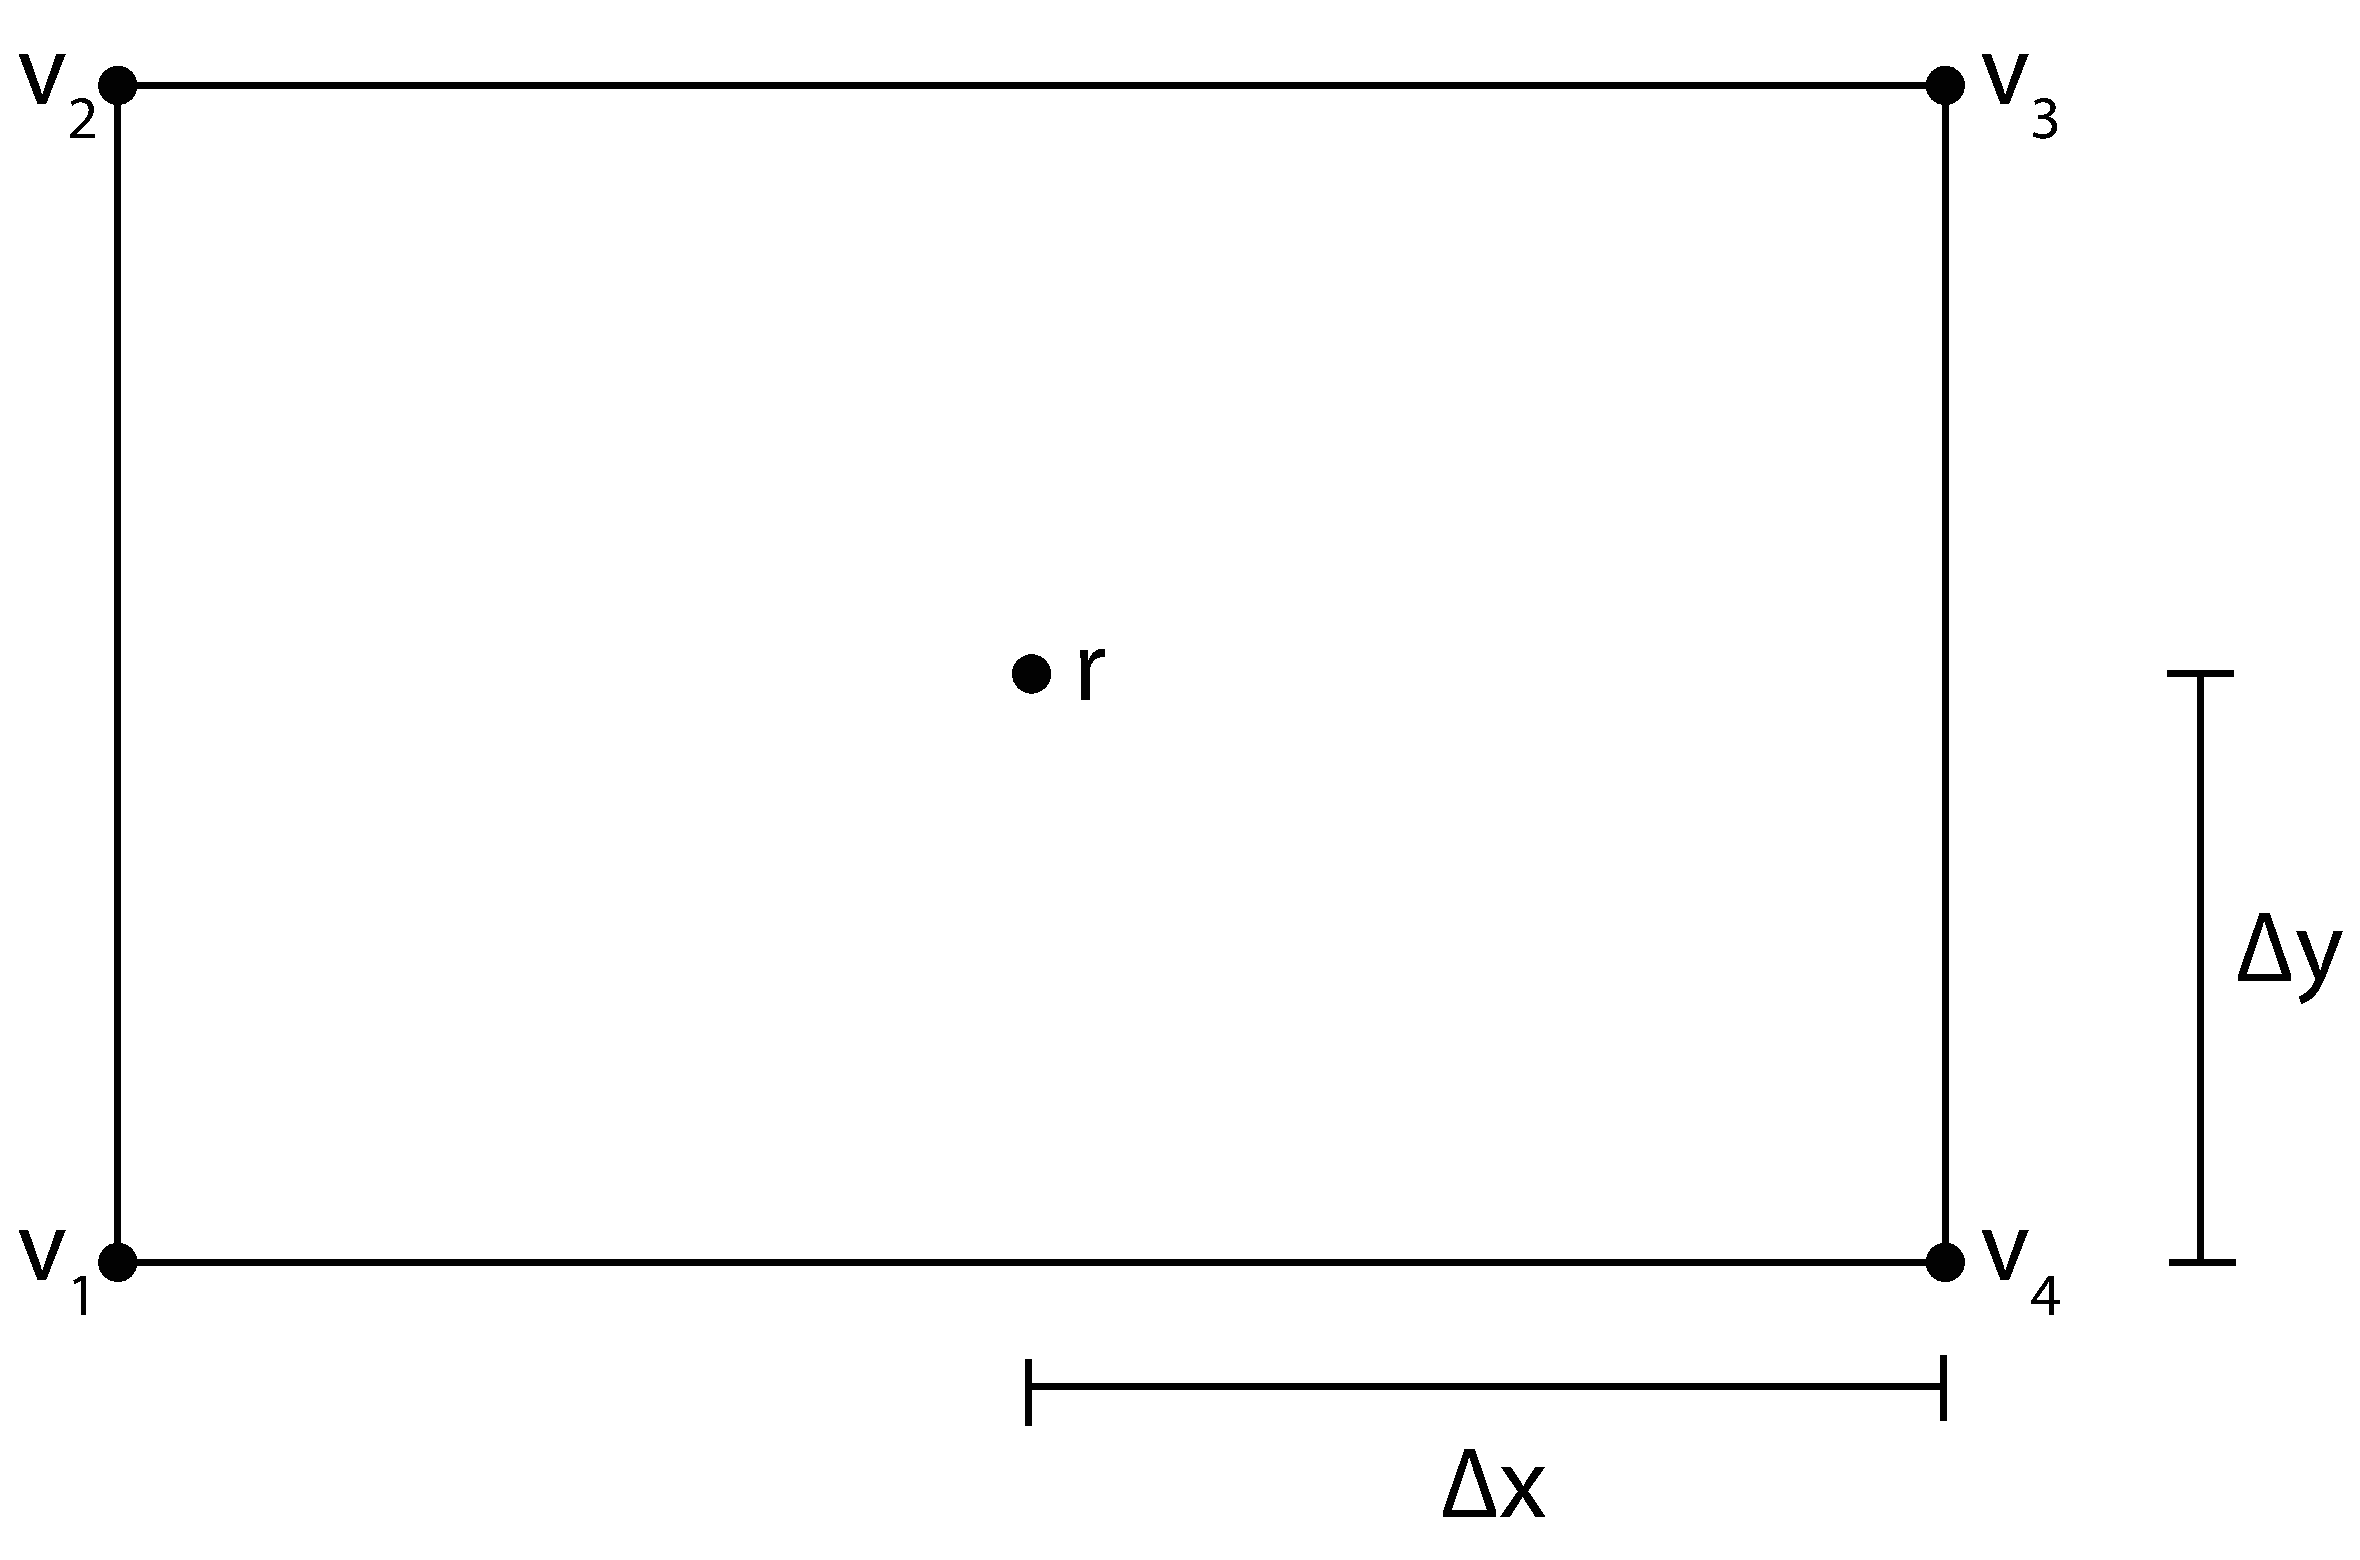
\includegraphics[width=0.7\textwidth, trim=0cm 0cm 0cm 0cm, clip]{visualization/figures/billboard.eps}
\end{center}
\caption{A billboard is made of four vertices $\vec v_1, \vec v_2, \vec v_3$ and $\vec v_4$ that can be calculated from one vertex $\vec r$ (equation \eqref{eq:vis_vertices_billboard}).}
\label{fig:visualization_billboard_vertices}
\end{figure}
This is already what Ovito does\footnote{See the source code at \url{http://www.ovito.org/index.php/download2}}, but we are going to improve this even more. Instead of computing the four vertices and uploading these as \textit{GL\_QUADS} to the GPU, we will only upload the positions of the particles, and exploit the geometry shader to create the billboard vertices on the GPU.\\
Before we start visualizing the data, all timesteps of a simulation are uploaded as VBO's on the GPU so that we don't need to upload data every frame. The VBO is rendered as \textit{GL\_POINTS} so each vertex represents the center position of a particle. We will now follow a single vertex through the pipeline
\subsection{The pipeline}
The VBO can now be seen as one OpenGL model containing the positions of all the particles. The vertices are then in the \textit{model space}. Every single vertex starts its life in the pipeline by going into the vertex shader. The vertex shader is pretty simple in this case, it just transforms the input vertex from the model space to the projection space as we can see in listing \ref{lst:simplevertexshaderbillboard}.
\begin{lstlisting}[caption=billboard\_vertex\_shader.glsl, label=lst:simplevertexshaderbillboard, 
#version 330\n"
uniform mat4 qt_ModelViewProjectionMatrix;
in vec4 qt_Vertex;
void main(void)
{
    gl_Position = qt_ModelViewProjectionMatrix * qt_Vertex;
}
\end{lstlisting}
This position is then sent to the geometry shader as an instance of the \textit{GL\_POINTS} primitive. The geometry shader will, from that single vertex (the position, now in the projection space), create and emit \textit{four} vertices that are displaced from the input vertex as explained in equation \eqref{eq:vis_vertices_billboard} and figure \ref{fig:visualization_billboard_vertices}. The size of the billboard is available as a uniform variable (as explained in subsection \ref{sec:opengl_uniforms}) in the geometry shader. If we want to visualize particles with different sizes (e.g. two atom types with different atomic radii), we just render different VBO's with the corresponding size. We want the four vertices to form a rectangle pointing towards the camera, so the operation in equation \eqref{eq:vis_vertices_billboard} should be done in the view space (here the $z$-direction is orthogonal on the camera plane which forms the $xy$-plane). Since the position vertex now is in the projection space, we should transform the four displacement vectors to the projection space by applying the \textit{qt_ProjectionMatrix} before we add them together. We then set the texture coordinate (the local coordinate in the texture image) on each vertex and emit it with the \textit{EmitVertex()} function. The algorithm might be easier to understand with a code example, see listing \ref{lst:simplegeometryshaderbillboard}.
\begin{lstlisting}[caption=billboard\_geometry\_shader.glsl, label=lst:simplegeometryshaderbillboard, language=GLSL]
#version 400
layout( points ) in;
layout( triangle_strip, max_vertices = 4 ) out;
uniform mat4 qt_ProjectionMatrix;
uniform vec2 size;
out vec2 texCoord;

void main(void) {
    vec4 pos = gl_in[0].gl_Position;
    gl_Position = pos + qt_ProjectionMatrix*vec4(-size.x, -size.y, 0.0, 0.0);
    texCoord = vec2(0.0, 0.0);
    EmitVertex();
    gl_Position = pos + qt_ProjectionMatrix*vec4(-size.x, size.y, 0.0, 0.0);
    texCoord = vec2(0.0, 1.0);
    EmitVertex();
    gl_Position = pos + qt_ProjectionMatrix*vec4(size.x, -size.y, 0.0, 0.0);
    texCoord = vec2(1.0, 0.0);
    EmitVertex();
    gl_Position = pos + qt_ProjectionMatrix*vec4(size.x, size.y, 0.0, 0.0);
    texCoord = vec2(1.0, 1.0);
    EmitVertex();
    EndPrimitive();
}
\end{lstlisting}
This is done with every single position vertex in the VBO (once per particle per frame) and all the output primitives from the geometry shader will be rasterized, clipped and texture coordinates are interpolated into the fragment shader that is run once per pixel per visible primitive. Before we discuss the fragment shader, we should take a look at the texture that each billboard will have.\\
We didn't lie before, we will use a circle that actually is a real sphere rendered in the 3D modeling program Blender\footnote{See \url{http://www.blender.org/} for details}. With some lighting, we get this nice shiny effect making the \"spheres\" look more interesting. This texture is shown in figure \ref{fig:visualization_billboard_texture}, where we also see that all the pixels outside the circles are transparent. This is very important so that we can discard these contributions in the fragment shader.
\begin{figure}[h]
\begin{center}
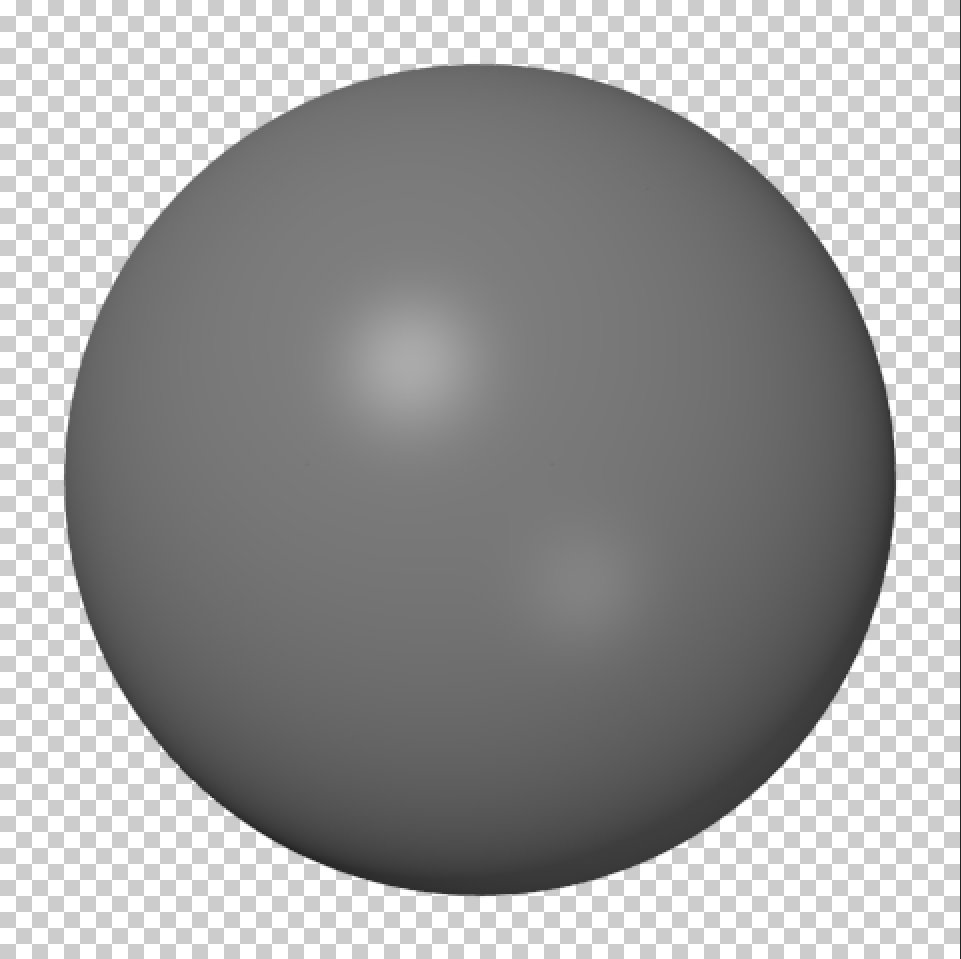
\includegraphics[width=0.7\textwidth, trim=0cm 0cm 0cm 0cm, clip]{visualization/figures/texture_transparent.png}
\end{center}
\caption{The texture used on the billboards is a circle which is a real sphere rendered with Blender. Notice that the pixels outside the circle are transparent. This allows us to discard these texture pixels in the fragment shader.}
\label{fig:visualization_billboard_texture}
\end{figure}
The fragment shader will then get an interpolated texture coordinate as input which we will use to look up which value this pixel gets from the texture. Now is the time for another detail, the color of the particles. Again we assume that all particles have the same color, so as the size variable, it is available as a uniform variable. The final pixel color is then found by equation \eqref{eq:opengl_combining_colors_textures}
\begin{align}
	\vec C(\vec p) = \vec c_t[\vec t(\vec p)] \odot \vec c(\vec p).
\end{align}
The fragment shader code is shown in listing \ref{lst:simplefragmentshaderbillboard} with the final rendering result in figure \ref{fig:visualization_billboard_md}. In this rendered image, we also added light effects making atoms that are far away from the camera appear darker. This increases the feeling of depth which clarifies the pore structures.
\begin{lstlisting}[caption=billboard\_fragment\_shader.glsl, label=lst:simplefragmentshaderbillboard, language=GLSL]
#version 330
uniform vec4 color;
uniform sampler2D qt_Texture0;
in vec2 texCoord;
out vec4 MyFragColor;

void main(void) {
    MyFragColor  = texture2D(qt_Texture0, texCoord.st);
    MyFragColor  = MyFragColor * color;
    if(MyFragColor.a < 0.9999) {
        discard;
    }
}

\end{lstlisting}

\begin{figure}[h]
\begin{center}
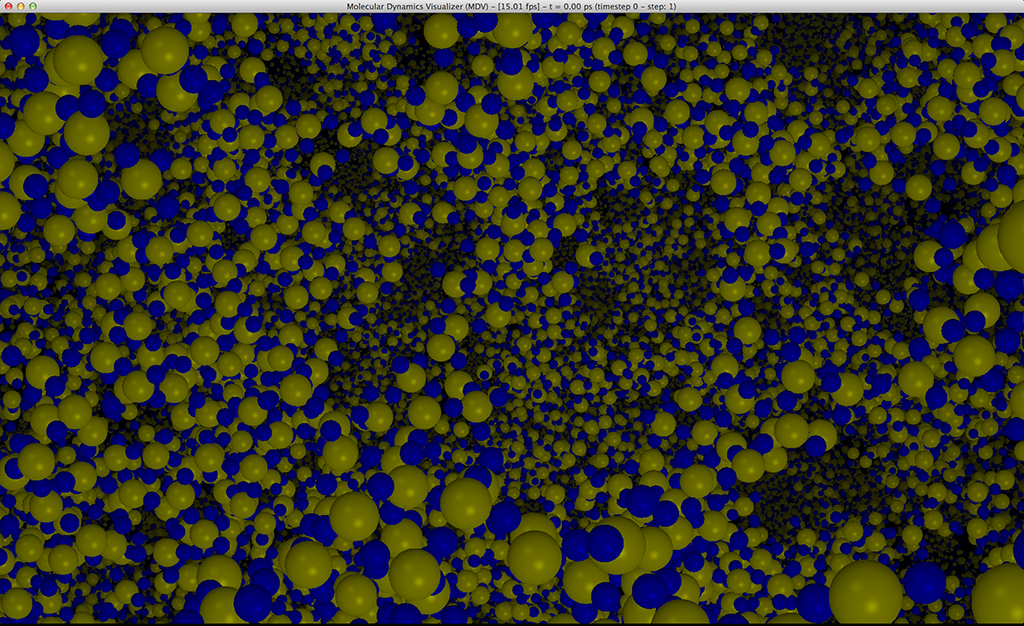
\includegraphics[width=\textwidth, trim=0cm 0cm 0cm 0cm, clip]{visualization/figures/billboards_md_visualization.png}
\end{center}
\caption{The final rendering result with an MD simulation using billboards. In the rendering, light effects are added to increase the depth feeling clarifying the pore structure. This system is a nanoporous SiO2 system simulated with the REMD22 code developed at USC.}
\label{fig:visualization_billboard_md}
\end{figure}

\subsection{Periodic copies}

    \section{Marching cubes}
\label{sec:marching_cubes}
The geometry in DSMC is represented as voxels as we discussed in section \ref{sec:dsmc_complex_geometries}. They form a scalar field with values zero for empty voxels, and non-zero for filled voxels. The surface of the geometry is where the values of the scalar field \textit{changes} from zero to a non-zero value. This defines the \textit{iso-surface}, i.e. a surface where all the values on one side is zero, and non-zero on the other side. If we find a way to visualize this iso-surface, it will coincide with where the DSMC particles collide. We then need to create some primitives (in this case triangles) that are connected to each other forming a the full iso-surface. Luckily for us, such an algorithm exists and is called \textit{marching cubes}.

Marching cubes is an algorithm used to generate a set of connected triangles from the iso-surface of a scalar field. The method was presented in a paper published in 1987 and has been widely used in medical visualizations of CT and MRI scans\cite{wiki:marching_cubes}. Assuming that the scalar field is discretized in space, each point (vertex) either has a value larger than some chosen iso-value, or a smaller value. Given a cube consisting of eight of these vertices, there exists $2^{8}=256$ unique combinations (each vertex has two possibilities). Because of symmetries (a cube with only one vertex being larger than the iso-value has through rotations 8 different configurations that really are the same configuration), this set can be reduced to 15. In figure \ref{fig:vis_marching_cubes}, we see the 15 unique configurations and the corresponding triangles in each configuration.
\begin{figure}[h]
\begin{center}
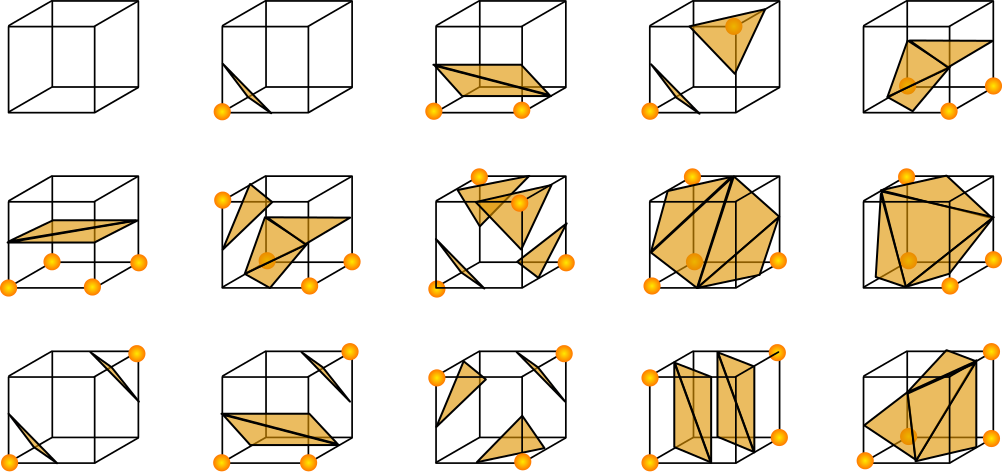
\includegraphics[width=\textwidth, trim=0cm 0cm 0cm 0cm, clip]{visualization/figures/marching_cubes.png}
\end{center}
\caption{A cube consisting of eight vertices, each having a value smaller or larger than a given iso-value has $2^8=256$ different combinations. This number can due to symmetries be reduced to 15 as we see here. (Image from \url{http://en.wikipedia.org/wiki/File:MarchingCubes.svg}, accessed 20 March, 2014.)}
\label{fig:vis_marching_cubes}
\end{figure}
For a given cube, the 8 vertex values (one or zero) can be represented as the bits in an 8-bit integer. The final value of this integer is then the index of a precomputed table containing a list of all triangles needed for that configuration. Well, the authors thought the 15 combinations would be enough, but it turns out that with these 15 configurations, there exists cases where the surface gets holes. This is topologically incorrect (the surface should not have any holes). This problem was solved in 1995 by using a larger set with 33 unique configurations which spans out the full configuration space \cite{chernyaev1995marching}.

Since the geometry in DSMC model is described by a scalar field with values zero, one and two, we can choose iso-value of one and use the marching cube algorithm to generate triangles we can render on the GPU. \todo{finish me}
    \section{Gallery}
    %\section{Oculus Rift}
\label{sec:oculus_rift}
  \end{chapter}
\end{part}

\begin{part}{Conclusion and discussion}
\begin{chapter}{Summary and conclusion}
\section{Summary}
After having explained and discussed all models and the results we have gathered during our work, it is convenient to briefly summarize the whole thesis. The main physical problem we discussed in the beginning was shale gas extraction. In the fracking process, the gas is released from everywhere in the shales through small pore networks, small channels with diameter from a few nanometers and up. Standard hydrodynamics breaks down at this scale because of non-continuum effects in addition to slip velocity, so we needed a model allowing us to study gas dynamics at this scale. In chapter \ref{chap:kinetic_theory} we briefly discussed statistical mechanics and kinetic theory, and used this to derive the Boltzmann equation, the mean free path and the mean collision time. These results were used to justify the assumptions the DSMC model in chapter \ref{chap:dsmc}. We explained how the model was implemented in chapter \ref{chap:dsmc_implementation}. With the parallel implementation and the voxel-based representation of arbitrary geometries, we managed to achieve the first two goals in subsections \ref{goal:dsmc_1} and \ref{goal:dsmc_2}.\\
In chapter \ref{chap:dsmc_results}, we discussed the simulations we performed with both model validation, performance tests and permeability analysis. We confirmed that the Knudsen correction from section \ref{sec:knudsen_correction} predicted the permeability very well for cylinders with a well defined Knudsen number. In the case of packed spheres, where the Knudsen number is less obvious how one would define due to statistical spread in the geometrical formation of the spheres, we found that an expectation value of the pore size could be used to find what we called an estimated Knudsen number (see appendix \ref{app:knudsen_number_packed_spheres}). We were able to predict the permeability to the correct order of magnitude, but the geometrical statistical spread was reflected through a spread in the final measured permeability. The ratio between the largest measured permeabilities and the smallest ones were a factor two or more, which greatly affects the economic outcome of gas extraction.\\
We then moved on to discuss MD with an introduction to the model in chapter \ref{chap:md}. The numerical implementation was explained in detail in chapter \ref{chap:md_implementation}. We also introduced a new model for simulating fluids confined by a solid that both interacted with realistic atomic forces and remained a solid with the initial geometry by adding a harmonic oscillator potential on the atoms. The rather short chapter with results (a lot of the discussions on concepts were already done in the DSMC results chapter), chapter \ref{chap:md_results}, showed that the parallel implementation scaled satisfactory up to at least one thousand processors. We also ran the MD program to measure the permeability in a cylinder for different Knudsen numbers, just like we did with DSMC. By simulating a similar system, but with a model based on different physical fundaments, this is a good way to validate the Knudsen correction for both different length scales and a large range of Knudsen numbers. In MD, the cylinder was 30 times smaller than in DSMC, with results confirming that the Knudsen correction works very well also for pores as small as 15 nanometers. With this, the goals in subsections \ref{goal:md_1} and \ref{goal:knudsen} were achieved. We will get back to the Knudsen correction in the discussion section below. We did not manage to implement the water-silica potential in MD as we wanted to do in subsection \ref{goal:md_2}. This would allow us to study flow in more realistic systems than with the Lennard-Jones potential we used.
\\
In the last part of the thesis, the custom 3d visualization tool, we first gave an introduction to OpenGL and its purpose in chapter \ref{chap:opengl}. We discussed the basics of graphics programming as well as the more advanced, important parts of the rendering pipeline that allowed us to develop an extremely efficient visualization program to visualize large particle data sets where tens of million atoms can be rendered realtime with a good framerate. This was possible by using billboards and geometry shaders, explained in chapter \ref{chap:particle_visualizer} with a final show-off gallery in the very last section \ref{sec:vis_gallery}. We have then obtained the goal in subsection \ref{goal:vis}.
\section{Discussion}
We have used two fundamentally different models to study flow in similar systems. MD is an atomic model computing forces between every atom whereas DSMC is a stochastic particle model based on statistical mechanics. Studying a physical problem this way has a great strength; when two models with different assumptions agree on the results, we have, to a greater extent, reasons to trust them than if it was just one model. But in any model, we make assumptions, and these may produce wrong answers. The main reason to use DSMC rather than MD is of course the reduced computational cost. The more physics you include in a model, the more computational expensive it is. This leads to the fundamental problem we always meet with before choosing a model - what is the physical problem, and what are the relevant phenomena?\\
A complete model of shale gas extraction should include physics describing both the gas production in the nanometer pores as well as the large scale flow from the fractures into the drilling hole. Today we do not have any good models covering the huge range in length scales and time scales. The models we have studied have indeed shown promising results predicting permeabilities in nanopores, but there might be other important effects we have not included in the models. For example, if the surfaces inside the pores have a non-zero net charge, it could significantly affect the fluid flow and the permeability. The model we used to create a solid in MD used a harmonic oscillator potential to keep the atoms at approximately the same position as they started. While this model includes realistic atomic forces and vibrations inside the solid, deformations and fracturing is impossible since the atoms are forced in the original formation.\\
It is assumed that the gas is trapped both inside already existing pores as well as adsorbed onto the organic material inside the shales. The rate of desorption from the organic material may require additional models releasing the gas from the organic material to the fracture network. It is needless to say that the models we have used are not complete in any sense. \\
From the theoretical perspective, we used the Knudsen correction to predict permeabilities in geometries with a closed form solution for the permeability at the no-slip scale - the absolute permeability. If we work with a geometry without a known absolute permeability, we can measure this in the high density limit and still use the Knudsen correction to predict permeabilities for dilute gases. The correction factor is a function of the Knudsen number, which is a well defined quantity in simple geometries like a cylinder. However, for more complicated geometries like the packed spheres, the Knudsen number should rather be seen as a distribution than one single number. It is possible, as we discuss in appendix \ref{app:knudsen_number_packed_spheres}, to calculate a distribution of Knudsen numbers providing both the mean value and the standard deviation which may be used to develop a \textit{stochastic} Knudsen correction based on the original model. 
\section{Rap}
Our thugged-out asses have used two fundamentally different models ta study flow up in similar systems. MD be a atomic model computin forces between every last muthafuckin atom whereas DSMC be a stochastic particle model based on statistical mechanics. Right back up in yo muthafuckin ass. Studyin a physical problem dis way has a pimped out strength; when two models wit different assumptions smoke on tha thangs up in dis biatch, our crazy asses have, ta a pimped outer extent, reasons ta trust dem than if dat shiznit was just one model. But up in any model, we make assumptions, n' these may produce wack lyrics. Da main reason ta use DSMC rather than MD iz of course tha reduced computationizzle cost. This points up a blingin fact; tha mo' physics you include up in a model, tha mo' computationizzle high-rollin' it is. This leadz ta tha fundamenstrual problem we always hook up before choosin a model; what tha fuck is tha physical problem, n' what tha fuck is tha relevant phenomena?

A complete model of shale gas extraction should include physics describin both tha gas thang up in tha nanometer pores as well as tha big-ass scale flow from tha fractures tha fuck into tha drillin hole. Todizzle our phat asses aint gots any phat models coverin dis big-ass range up in length scalez n' time scales. On tha larger scale, we use continuum mechanics whereas tha smalla scale requires models like MD or DSMC. On tha smallest scale there be nuff muthafuckin alternatives ta these two. Other ghettofab methodz is tha lattice Boltzmann (LB), dissipatizzle particle dynamics (DPD), which both can simulate larger systems fo' lager times. But again, a gangbangin' fasta model probably includes less physics fo' realz. A comparison between DSMC n' these models would be interesting.

Both models our crazy asses have studied have indeed shown promisin thangs up in dis biatch, calculatin permeabilitizzles up in nanopores up in agreement wit tha Knudsen erection yo, but there might be other blingin effects we aint included up in tha models. Right back up in yo muthafuckin ass. Such effects is probably not incorporated up in tha Knudsen erection either yo, but could become evident up in a experiment. Validation of a model aint necessarily a validation of tha assumptions. For example, if tha surfaces inside tha pores gotz a non-zero net charge, it could hella affect tha fluid flow n' tha permeability. We can incorporate dis up in MD by rockin a mo' advanced potential. It aint nuthin but tha nick nack patty wack, I still gots tha bigger sack. Da model we used ta create a solid up in MD used a harmonic oscillator potential ta keep tha atoms at approximately tha same posizzle as they started, keepin tha geometrical form of tha solid. Y'all KNOW dat shit, muthafucka! While dis model includes realistic atomic forces n' vibrations inside tha solid, deformations n' fracturin is now impossible since tha atoms is forced up in tha original gangsta formation.

It be also assumed dat tha gas is trapped both inside already existin pores as well as adsorbed onto tha organic material inside tha shales. Da rate of desorption from tha organic material may require additionizzle models releasin tha gas from tha organic material ta tha fracture network. These is just a gangbangin' few yo, but blingin remarks bout tha limitationz of tha models. Well shiiiit, it is needless ta say dat they is not complete up in any sense. Even if they \textit{were} complete, if they calculated both gas thang n' flow from tha smallest pores tha fuck into tha fracture network, we would not be even close ta a cold-ass lil complete model of a shale reservoir. Shiiit, dis aint no joke. Da couplin between different length scalez - multi scale physics - is still a unsolved problem up in physical science.

From tha theoretical perspective, we used tha Knudsen erection ta predict permeabilitizzles up in geometries wit a cold-ass lil closed form solution fo' tha absolute permeabilitizzle all up in tha no-slip scale. If we work wit a geometry without a known absolute permeability, we can measure dis up in tha high densitizzle limit, n' still use tha Knudsen erection ta predict permeabilitizzles fo' dilute gases. Da erection factor be a gangbangin' function of tha Knudsen number, which be a well defined quantitizzle up in simple geometries like a cold-ass lil cylinder n' shit. But fuck dat shiznit yo, tha word on tha street is dat fo' mo' fucked up geometries like tha packed spheres, tha Knudsen number should rather be peeped as a gangbangin' finger-lickin' distribution than one single number n' shit. Well shiiiit, it is possible, as our phat asses say shit bout up in appendix \ref{app:knudsen_number_packed_spheres}, ta calculate a gangbangin' finger-lickin' distribution of Knudsen numbers providin both tha mean value n' tha standard deviation which may be used ta pimp a \textit{stochastic} Knudsen erection based on tha original gangsta model. By obtainin statistical shiznit bout tha geometry of a real shale reservoir, such a theory could up in principle enable our asses ta do a economical risk analysis based on tha permeabilitizzle distribution. I aint talkin' bout chicken n' gravy biatch. 
\section{Future work}
No matter how much work we do, new ideas pop our minds faster than we manage to complete the old ones. During the past months, through everything we have learned, both ideas about extensions to the models and applications have emerged. First of all, as we discussed in section \ref{sec:dsmc_steady_state}, our analysis of whether or not the system has reached a steady state is inadequate. New, automatic methods should be incorporated by, in several regions (for example by using the collision cells in DSMC), looking at expectation values and the variance of physical quantities such as momentum, energy and temperature. Even with a more advanced analysis of if the steady state is reached or not, reaching a steady state may take a long time. In the benchmark we performed and discussed in section \ref{sec:dsmc_parallelization_performance}, 512 processors used 545 seconds to proceed 500 timesteps with one billion particles. If the system requires 100k timesteps to reach a steady state, this would require 15k cpu hours just to reach the steady state. With DSMC, it may be possible to use a smaller number of particles (that is, increase the number of effective atoms per simulated particle) while the system reaches a steady state. Then, before the sampling, increase the total number of particles by distributing a number of particles with the velocities and densities computed from the previous simulation, equilibrating this state before starting the sampling.\\
A detailed study of how the Cercignani-Lampis collision model from section \ref{sec:surface_interactions} affects the permeability would also be a interesting and important work. Here one could for example also use the Lennard-Jones MD model to fire single atoms towards a surface and gather a distribution to compare with the Cercignani-Lampis model.\\
With the voxelization model of the surface we developed in section \ref{sec:dsmc_complex_geometries} a few questions quickly arise. What are the effects of the discretization of the geometry? A real, smooth surface does indeed look different than a jagged surface composed by voxels. With this representation, the effective surface area is increased which could affect the flow. A detailed study of these effects should be carried out. Such a representation also requires a lot of memory as the memory requirement scales as $O(N^3)$. To save memory, we can use a sparse voxel octree representation. If a larger group of voxels all share the same value, only one, larger voxel is saved in memory, representing all the smaller voxels.\\
For a large number of processors, the amount of work each processor is assigned may not be equal to all the others. This means that a processor that is computing only half the work than another processor, it will spend 50$\%$ of its time waiting for the other processors to finish. The solution to this is known as load balancing. An analysis of the system prior to the simulation may distribute the amount of work not by dividing the system into equal \textit{total volumes}, but equal \textit{pore volumes} in which the particles are. The amount of work is proportional to the number of particles a processor has.\\


Large system state preparation
Diffusion on the matrix
Deformations and fracking
Permeability of real materials
\end{chapter}
\end{part}
%---------------------------------------------------------------------------------------
% Appendices
%---------------------------------------------------------------------------------------
\begin{part}{Appendices}
\begin{appendices}
\chapter{Knudsen number of a packed spheres system}
\label{app:knudsen_number_packed_spheres}
If we want to use the Knudsen correction factor (equation \eqref{eq:knudsen_correction}) to predict permeabilities in a nanoporous system consisting of packed spheres, we need to derive some statistical properties of the system giving us enough information to calculate the expected Knudsen number. Now, consider a volume $V$ consisting of $N$ points (sphere centers) placed randomly and independently in the system. Note that this allows spheres with radius $r$ to overlap. The density of points is of course given by
\begin{align}
	\label{eq:packed_sphere_density}
	n = \frac{N}{V}.
\end{align}
The probability of placing a sphere center in a volume $v$ is $v/V$, yielding the probability of \textit{not} placing a sphere center in that same volume $(1 - v/V)$. If we now place $N$ such points, the probability $P_0(N)$ of not having placed \textit{any} points in that volume is given by
\begin{align}
	P_0(N) = \left[1 - \frac{nv}{N}\right]^N,
\end{align}
where we have used that $v/V = nv/nV = nv/N$ using equation \eqref{eq:packed_sphere_density}. In the limit where $N\rightarrow\infty$ and $V\rightarrow\infty$, keeping the density $n$ and $v$ constant, the probability approaches
\begin{align}
	P_0 = \lim_{N\rightarrow\infty}\left[1 - \frac{nv}{N}\right]^N = \exp(-nv).
\end{align}
We can use this to compute the probability of finding \textit{no} sphere centers within a distance $l$ from a point
\begin{align}
	\label{eq:packed_sphere_p0}
	P_0(l) = \exp\left(-\frac{4n\pi}{3}l^3\right),
\end{align}
where we just used the volume of a sphere $v=4/3\pi l^3$. This is the cumulative probability distribution of finding \textit{no} sphere centers within a distance $l$, so the inverse problem, the probability of finding \textit{at least one} sphere center at some distance $x<l$ is now easy to calculate 
\begin{align}
	P(x<l) = 1 - \exp\left(-\frac{4n\pi}{3}l^3\right).
\end{align}
This is also a cumulative distribution function which we can differentiate to find the probability distribution of distances $l$
\begin{align}
	\label{eq:packed_sphere_probability_number_density}
	p(l) = 4\pi n l^2 \exp\left(-\frac{4n\pi}{3}l^3\right).
\end{align}
$p(l)\dm l$ is the probability of finding a sphere center within the range $[l, l+\dm l)$. In this calculation, we are only interested in the distribution of distances $l$ \textit{given that we are not inside any spheres}. So we define a new distribution function
\begin{align}
	q(l) = \left\{\begin{array}{l l}
			0 & \text{if $l<r$},\\
			Mp(l) & \text{if $l\geq r$},
			\end{array}\right.
\end{align}
where $M$ is the normalization constant for $q(l)$ (the area must be less than one now since we removed all the points from zero to $r$). We find $M$ by integrating
\begin{align}
	1 &= M\int\limits_0^\infty q(l)\dm l = M\int\limits_r^\infty p(l)\dm l\\
	&= M4\pi n\int\limits_r^\infty l^2 \exp\left(-\frac{4n\pi}{3}l^3\right) \dm l\\
	&= M\exp\left(-\frac{4n\pi}{3}r^3\right),
\end{align}
which gives $M=\exp\left(\frac{4n\pi}{3}r^3\right)$. Avoiding the points being inside the spheres is of course the same as choosing only the points that are in the pore space. The probability of randomly choosing such a point is actually the porosity $\phi$ (remember, the porosity is pore space volume divided by total volume). It is found by using equation \eqref{eq:packed_sphere_p0}
\begin{align}
	\label{eq:packed_sphere_porosity}
	\phi = \exp\left(-\frac{4n\pi}{3}r^3\right),
\end{align}
which we recognize as $M^{-1}$. We can then rewrite $q(l)$
\begin{align}
	q(l) = \left\{\begin{array}{l l}
			0 & \text{if $l<r$},\\
			4n\pi\phi^{-1} l^2 \exp\left(-\frac{4n\pi}{3}l^3\right) & \text{if $l\geq r$}.
			\end{array}\right.
\end{align}
Now it would be interesting to find the average distance to the sphere centers. It is found by calculating
\begin{align}
	\langle l\rangle &= \int\limits_r^\infty lq(l) \dm l = \frac{4n\pi}{\phi}\int\limits_r^\infty l^3 \exp\left(-\frac{4n\pi}{3}l^3\right) \dm l \\
	\label{eq:packed_sphere_average_distance}
	&= \sqrt[3]{\frac{3}{4n\pi}}\frac{1}{\phi}\Gamma\left(\frac{4}{3}, \frac{4n\pi}{3}r^3\right),
\end{align}
where $\Gamma(a,x)$ is the incomplete gamma function defined as
\begin{align}
	\Gamma(a,x) = \int\limits_x^\infty t^{a-1}\exp(-t)\dm t.
\end{align}
We can use equation \eqref{eq:packed_sphere_porosity} to replace the dependency of the number density $n$ with the porosity $\phi$ and sphere radius $r$ by solving for $n$ 
\begin{align}
	n = \frac{3}{4\pi r^3} \ln\phi^{-1},
\end{align}
and then insert this into equation \eqref{eq:packed_sphere_average_distance} to obtain
\begin{align}
	\langle l(r,\phi) \rangle = \frac{r}{\phi}\left[\ln\phi^{-1}\right]^{-\frac{1}{3}}\Gamma\left(\frac{4}{3},\ln\phi^{-1}\right).
\end{align}
What we really want is the distances to the \textit{surfaces} of the spheres, $d=(l-r)$ which is easy to find
\begin{align}
	\langle d(r,\phi)\rangle &= \langle l(r,\phi)\rangle - r = \frac{r}{\phi}\left[\ln\phi^{-1}\right]^{-\frac{1}{3}}\Gamma\left(\frac{4}{3},\ln\phi^{-1}\right) - r\\
	&= r\left[\phi^{-1}\left[\ln\phi^{-1}\right]^{-\frac{1}{3}}\Gamma\left(\frac{4}{3},\ln\phi^{-1}\right) - 1\right].
\end{align}
In the expression for the Knudsen number ($\text{Kn}=\lambda/L$), we will use this quantity instead of $L$ as our best estimate, or average value, of the channel diameter. We then define the estimated Knudsen number $\text{Kn($r,\phi$)}^*$ as
\begin{align}
	\text{Kn($r,\phi$)}^* &= \frac{\lambda}{\langle l(r,\phi)\rangle}\\
	\label{eq:packed_sphere_estimated_knudsen}
	&= \frac{\lambda}{r\left[\phi^{-1}\left[\ln\phi^{-1}\right]^{-\frac{1}{3}}\Gamma\left(\frac{4}{3},\ln\phi^{-1}\right) - 1\right]}.
\end{align}
\chapter{The Liouville operator and time integrators}
\label{app:liouville}
The derivation of time integrator schemes are usually done in a mathematical sense using Taylor expansions. Given a Taylor expansion $f(x+h) = f(x) + hf'(x) + h^2/2f''(x) + ...$, we often truncate at some term, yielding a truncation error $O(h^n)$. In physics, there are other properties of a system of which the error doesn't scale as the truncation error. A typical example is the energy of a particle system. Two different time integrators may have the same truncation error, but have very different long term behavior if one has a drift in the energy whereas the other doesn't.\\
There are other properties that might be difficult to measure through a mathematical analysis of the Taylor expansion that may be more important than the truncation error itself. In the Hamiltonian formulation of classical mechanics, we obtain the equations of motion through the energy operator $\vec H = \vec T + \vec V$, where $\vec T$ and $\vec V$ are operators measuring the kinetic and potential energy. Using the physical description of a system can help developing better integration schemes. \\
In this chapter we will address the equations of motion by using the Liouville operator to derive a way to create time integration schemes. We start by looking at the phase space coordinates and define the Liouville operator in section \ref{sec:liouville_operator}. We then define the time evolution operator and split the Liouville operator into two operators; one operator acting on the positions and one acting on the momenta.  These operators do not commute, so we use the Trotter identity to introduce time discretization and derive the Velocity Verlet algorithm, which is the one used in the Molecular Dynamics code. We then do an analysis of the mathematical error to find the local error (which is the same as the truncation error) in section \ref{sec:velocity_verlet_error}. This derivation is done as in \cite{frenkel2001understanding}. In section \ref{sec:multiple_timestep_schemes} we use the Liouville formulation to derive a multiple timestep integration scheme that can be used if the Molecular Dynamics system consists of both light and heavy atoms. Light atoms like hydrogen need a small timestep in order to accurately integrate vibrations of high frequency, whereas the heavier atoms tolerate a higher timestep. 
\section{Liouville operator}
\label{sec:liouville_operator}
The physical system consists of $N$ particles, each having three positions and three momenta defining the phase space point $(\vec r, \vec p)$. Now assume some function of these variables $f(\vec r(t), \vec p(t)) = f(t)$ (the function is indirectly a function of time) that has the time derivative
\begin{align}
	\dot f(t) = \dot {\vec r}\frac{\partial f(t)}{\partial \vec r} + \dot {\vec p}\frac{\partial f(t)}{\partial \vec p} \equiv \liouville f(t),
\end{align}
where we have defined the Liouville operator
\begin{align}
	\liouville = \dot{\vec r}\frac{\partial }{\partial \vec r} + \dot{\vec p}\frac{\partial }{\partial \vec p}.
\end{align}
This allows us to define the time evolution operator $\hat{\mathcal U}(t)$
\begin{align}
	\label{eq:liouville_time_evolution}
	f(t) = \hat{\mathcal U}(t)f(0) = e^{\liouville t}f(0),
\end{align}
which is easily verified
\begin{align}
	\dot f(t) = \liouville \left[e^{\liouville t}f(0)\right] = \liouville f(t).
\end{align}
If we now split the Liouville operator into two parts
\begin{align}
	\liouville = \liouviller + \liouvillep,
\end{align}
so that
\begin{align}
	\liouviller = \dot{\vec r(0)}\frac{\partial }{\partial \vec r}.
\end{align}
Let us see what this operator can do if we insert it into equation \eqref{eq:liouville_time_evolution} and expand the exponential
\begin{align}
	f(t) &= \exp\left(\liouviller t\right) f(0)\\
	&= \exp\left(\dot{\vec r}t\frac{\partial }{\partial \vec r}\right)f(0)\\
	&= \sum_{n=0}^\infty \frac{(\dot{\vec r}(0)t)^n}{n!}\frac{\partial^n}{\partial \vec r^n} f(0)\\
	&= f\left[\left(\vec r(0) + \dot{\vec r}(0)t\right), \vec p(0)\right].
\end{align}
It does just what we expect it to do, it is a displacement operator, moving the points in the phase space according to their time derivative. The momentum Liouville operator does of course exactly the same, so that by applying the total time evolution operator, we do indeed get
\begin{align}
	f(t) &= e^{\liouville t}f(0) = f\left[\left(\vec r(0) + \dot{\vec r}(0)t\right), \left(\vec p(0) + \dot{\vec p}(0)t\right)\right].
\end{align}
If we were to use this in a simulation, we normally do not apply the full operator at the same time, we might first treat the positions, then the momenta. So ideally, we would want to first apply one operator, then the next one
\begin{align}
	e^{\liouville} = e^{\liouvillep + \liouviller} \neq e^{\liouvillep}e^{\liouviller},
\end{align}
but this is not the case since the operators do necessarily commute. However, for two operators $\vec A$ and $\vec B$, we can use the \textit{Trotter identity}\cite{frenkel2001understanding}
\begin{align}
	e^{A + B} = \lim_{N\rightarrow\infty}\left(e^{A/2M}e^{B/M}e^{A/2M}\right)^N,
\end{align}
which can be truncated
\begin{align}
	e^{A + B} = \left(e^{A/2N}e^{B/N}e^{A/2N}\right)^Ne^{O(1/N^2)}.
\end{align}
This can be used to derive different time integrator schemes. We will now derive the Velocity Verlet scheme which is used in the Molecular Dynamics code.
\section{Derivation of the Velocity Verlet algorithm}
The truncated Trotter identity is neat, we can replace $A$ with the $\liouvillep$ and $B$ with $\liouviller$
\begin{align}
	\frac{\liouvillep}{M} &\equiv \Delta t\dot{\vec p}(0)\frac{\partial}{\partial \vec p}\\
	\frac{\liouviller}{M} &\equiv \Delta t\dot{\vec r}(0)\frac{\partial}{\partial \vec r}
\end{align}
defining the timestep $\Delta t = t/N$. The truncated time evolution operator now reads
\begin{align}
	\hat {\mathcal U} (t) = \left(e^{\liouvillep \Delta t/2}e^{\liouviller \Delta t}e^{\liouvillep \Delta t/2}\right)^N
\end{align}
where we identify one timestep iteration
\begin{align}
	\hat {\mathcal U} (\Delta t) = e^{\liouvillep \Delta t/2}e^{\liouviller \Delta t}e^{\liouvillep \Delta t/2}.
\end{align}
If we now apply this operator on $f(0)$, we first apply the rightmost operator
\begin{align}
	e^{\liouvillep \Delta t/2}f\left[\vec p(0), \vec r(0)\right] = f\left\{\vec r(0), \left[\vec p(0) + \frac{\Delta t}{2}\dot{\vec p}(0)\right] \right\},
\end{align}
before applying $\exp(\liouviller t)$
\begin{align}
	e^{\liouviller t}f\left\{\vec r(0), \left[\vec p(0) + \frac{\Delta t}{2}\dot{\vec p}(0)\right] \right\}\\
	= f\left\{\left[\vec r(0) + \Delta t \dot{\vec r}(\Delta t/2)\right], \left[\vec p(0) + \frac{\Delta t}{2}\dot{\vec p}(0)\right] \right\}.
\end{align}
Our last operator gives the final result
\begin{align}
	f\left\{\left[\vec r(0) + \Delta t \dot{\vec r}(\Delta t/2)\right], \left[\vec p(0) + \frac{\Delta t}{2}\dot{\vec p}(0) + \frac{\Delta t}{2}\dot{\vec p}(\Delta t)\right] \right\}.
\end{align}
These steps can be summarized as one usually does with time integrators
\begin{align}
	\vec v(\Delta t/2) &= \vec v(0) + \frac{\vec F(0)}{m}\frac{\Delta t}{2}\\
	\vec r(\Delta t) &= \vec r(0) + \vec v(\Delta t/2)\Delta t\\
	\vec v(\Delta t) &= \vec v(\Delta t/2) + \frac{\vec F(\Delta t)}{m}\frac{\Delta t}{2},
\end{align}
where we have replaced $\dot{\vec p}$ with the equivalent $(\vec F/m)$ and $\dot{\vec r}$ with $\vec v$ which is valid if the forces can be calculated from the position. These steps are called the Velocity Verlet algorithm and has, as we now will see, an error $O(\Delta t^3)$.

\section{Truncation error}
\label{sec:velocity_verlet_error}
During one timestep iteration, we approximate the Liouville operator
\begin{align}
	e^{\liouville \Delta t} \approx e^{\liouvillep \Delta t/2}e^{\liouviller \Delta t}e^{\liouvillep \Delta t/2} = e^{\liouville \Delta t + \hat{\vec \epsilon}},
\end{align}
where we have introduced the \textit{error operator} $\hat{\vec \epsilon}$ that represents our truncation error. These are linear operators on which we can use the Campbell-Baker-Hausdorff expansion of general, non-commuting linear operators
\begin{align}
	e^{\lambda\hat{\vec A}}e^{\lambda\hat{\vec B}} = e^{\lambda\hat{\vec A} + \lambda\hat{\vec B} + \frac{\lambda^2}{2}[\hat{\vec A},\hat{\vec B}] + \frac{\lambda^3}{12}[\hat{\vec A},[\hat{\vec A},\hat{\vec B}]] + \frac{\lambda^3}{12}[\hat{\vec B},[\hat{\vec A},\hat{\vec B}]] + ...}
\end{align}
together with 
\begin{align}
	e^{\oper A}e^{\oper B} = e^{\oper B + [\oper A,\oper B] + \frac{1}{2!}[\oper A,[\oper A,\oper B]] + \frac{1}{3!}[\oper A,[\oper A,[\oper A,\oper B]]] + ...}e^{\oper A}
\end{align}
to find the leading term in $\hat{\vec \epsilon}$
\begin{align}
	-(\Delta t)^3\left(\frac{1}{24}[\liouviller, [\liouviller, \liouvillep]] + \frac{1}{12}[\liouvillep, [\liouviller, \liouvillep]]\right),
\end{align}
where we see that $\Delta t^3$ is the local truncation error in the Velocity Verlet algorithm. 
\section{Multiple timestep integration schemes}
\label{sec:multiple_timestep_schemes}
We will now address a situation that may occur in an advanced Molecular Dynamics simulation. Let's say we will simulate a system with several atom types, like silica and water. In such a system, we have both hydrogen, oxygen and silicon, which all may feel the appearance of all the other atom types. Hydrogen atoms are 28 times lighter than silicon. A consequence of this is that hydrogen will have much higher velocities than the other atom types, they will typically vibrate very quickly in the water molecules. This will require a much smaller timestep than those of the silicon and oxygen atoms would need. Long range forces like the Coulomb force are other examples of interactions that are accurate with higher timesteps. We will now use the Liouville formulation to derive a scheme that will allow multiple timesteps.\\
Again we split the Liouville operator into the sum of operators. \todo{Derive this.}
\chapter{Workflow and Python scripting}
When we are running simulations to study flow in nanoporous media, one single experiment consists of more than just starting the program and waiting for the result. A typical simulation scheme could be
\begin{enumerate}
	\item Prepare geometry
	\item Initialize system
	\item Reach a steady state
	\item Sample statistics.
\end{enumerate}
Some of these steps aren't even performed by the same c++ program, so we have developed a scripting framework in Python wrapping all the functionality from the different c++ programs into one scripting framework. This simplifies the workflow all the way from the very idea of some physical problem to running the simulation to study it. In this appendix we will discuss the Python framework and show the workflow of how to study problem, from idea to simulation, using DSMC.
\section{From idea to simulation}
\subsection{Create the geometry}
The program package we have developed is an excellent tool to study flow of dilute gases in complex nanoporous media. So what we usually do is to come up with the idea of some interesting geometry to study. This could either be a real sample dataset, a mathematical description or some other creative way to create the geometry. An example could be the packed spheres discussed in section \ref{sec:dsmc_packed_spheres_results} where each sphere is placed out randomly inside the volume defined by the $N_x\times N_y \times N_z$ voxel grid. All the voxels within a given distance (the sphere radius) from the sphere center are marked as solid voxels. Any other geometry can made with this technique with the code in the \textit{complexgeometry.cpp} file. 
\subsection{Initialize system}
Once we have the geometry of the system we would like to study, we need to insert gas particles inside the system. The gas could in principle have different densities based on position or other properties, but in this thesis we are placing the particles uniformly in the pore volume, i.e. in voxels marked as empty. We choose velocities from the Maxwell-Boltzmann distribution (equation \eqref{eq:maxwell_boltzmann_distribution}) so that the gas has the temperature we want.
\subsection{Reach a steady state}
Now that we have our gas particles inside the (possibly) complex geometry, we want to apply a pressure gradient inducing flow. In the beginning, all the particles are (on average) at rest, so we should wait until we have reached a steady state before we start sampling statistics. Methods to determine whether or not a system has reached a steady state was discussed in section \ref{sec:dsmc_steady_state}. 
\subsection{Sample statistics}
If we assume that the system finally has reached a steady state, we can start measuring the physical quantities discussed in section \ref{sec:dsmc_measuring_physical_quantities}. The main focus in this thesis has been to study the permeability for different geometries. 
\subsection{The run script - example.py}
Finally, after having defined all the steps in our scheme, we can gather everything into one single Python script. This example script shows how to perform all the steps discussed above. 
\begin{lstlisting}[caption=example.py, label=lst:dsmc_example_script, language=Python]
	from dsmcconfig import *
	from dsmc_unit_converter import *
	from dsmc_geometry_config import *
	nx = 2 # Number of processors in x-direction
	ny = 2 # Number of processors in y-direction
	nz = 2 # Number of processors in z-direction
	program = DSMC(dt=0.001, nx=nx, ny=ny, nz=nz)
	dsmc = program.compile(name="main")
	geometry = DSMC_geometry(program)
	unit_converter = DSMC_unit_converter(program)
	
	# Save geometry files to this directory
	geometry.binary_output_folder = "../geometries/example_geometry/"
	program.world = geometry.binary_output_folder
	
	# Set the dimensionality of the voxel grid
	geometry.num_voxels_x = 128
	geometry.num_voxels_y = 128
	geometry.num_voxels_z = 128
	
	#geometry.create_cylinders(radius=0.05, num_cylinders_per_dimension = 4)
	geometry.create_packed_spheres(radius = 0.02, spheres_type = 1, wanted_porosity = 0.5)
	
	# Specify the array size (maximum number of particles)
	program.max_molecules_per_node = 1.5e6
	
	# Set system size (in micro meters)
	program.Lx = 1
	program.Ly = 1
	program.Lz = 1
	
	# Select density (Kn = mean_free_path / length)
	program.density = unit_converter.density_from_knudsen_number(knudsen_number=1.0, length=program.Ly)
	
	# Prepare a new simulation, delete old files
	program.reset()
	
	# Select how many atoms each particle represents
	program.atoms_per_molecule = 1
	
	# Set the number of collision cells
	program.set_number_of_cells(geometry, particles_per_cell=100)
	
	# Initialize gas particles
	program.prepare_new_system()
	program.run(dsmc)
	
	# Apply pressure gradient
	program.apply_pressure_gradient_percentage(factor=2.0)
	
	# Select low statistics measuring interval
	program.statistics_interval = 10000
	# Select num timesteps to reach steady state
	program.timesteps = 500000
	
	program.create_config_file()
	program.run(dsmc)
	
	# Select high statistics measuring interval
	program.statistics_interval = 100
	# Select num timesteps to sample
	program.timesteps = 100000
	
	program.create_config_file()
	program.run(dsmc)
}
\end{lstlisting}
\section{The Python framework}
\chapter{Physical units}
The choice of units does of course not change the physical behavior. It is only a scaling of the the physical quantities so that their numerical values become more convenient. For example, it is common to choose a unit of length $L_0$ so that one unit of length is a typical value in the physical system. There are however only a few \textit{free} choices of units of which the other units follow from. In this appendix, we discuss the choices of units in both the MD and DSMC simulations and derive the other units.
\section{Choice of units in MD}
Here we use the so-called MD units. A convenient consequence of these units are that the parameters and masses in the Lennard-Jones force can be factored out which gives simpler calculations. The units we choose are
\begin{align}
	\text{Length } L_0 &= \unit{3.405\e{-10}}{\meter},\\
	\text{Mass } m_0 &= \unit{1.66053886\e{-27}}{\kilogram},\\
	\text{Energy } E_0 &= \unit{1.65088\e{-21}}{\joule},\\
	\text{Boltzmann constant } k_B^* &= 1.0.
\end{align}
\section{Choice of units in DSMC}
In DSMC, we use the same initial units as in MD, but with another unit of length since the systems normally are a few orders of magnitude larger. Here we use
\begin{align}
	\text{Length } L_0 &= \unit{1.0\e{-6}}{\meter},\\
	\text{Mass } m_0 &= \unit{1.66053886\e{-27}}{\kilogram},\\
	\text{Energy } E_0 &= \unit{1.65088\e{-21}}{\joule},\\
	\text{Boltzmann constant } k_B^* &= 1.0.
\end{align}
Note that the mass, energy and the Boltzmann constant are equal in both MD and DSMC. 
\section{Derivation of the other units}
The other units can be derived from the four basis units through relations like $E=mc^2$ and $P=F/A$. Together, these physical formulas form a set of equations that can be solved for each physical quantity. We find the time unit $t_0$ through $E=mc^2$
\begin{align}
	E0 = m_0\frac{L_0^2}{t_0^2}\\
	t_0 = L_0\sqrt\frac{m_0}{E_0}.
\end{align}
The force unit $F_0$ is found by using Newton's second law
\begin{align}
	F_0 = \frac{m_0L_0}{t_0^2} = \frac{E_0}{L_0}
\end{align}
We find the temperature $T_0$ by using that we chose the Boltzmann constant to be 1.0, which gives
\begin{align}
	T_0 = \frac{E_0}{k_B}.
\end{align}
The pressure is found through $P=F/A$ \todo{check this}
\begin{align}
	P_0 = \frac{F_0}{L_0^2} = \frac{E_0}{L_0^3}.
\end{align}
Now we have all all the conversion factors between SI units and MD/DSMC units. The programs are written so that all input values and internal variables are in the MD/DSMC units, but we have a simple unit converter script that can transform any physical value both to and from SI units. The conversion script can be found in listing \ref{lst:dsmcunitconverter}.
\begin{lstlisting}[caption=dsmcUnitConverter.py, label=lst:dsmcunitconverter, language=Python]
from dsmcconfig import *
from math import sqrt, pi

class DSMC_unit_converter:
	def __init__(self, dsmc):
		self.dsmc = dsmc
		self.m0 = 1.66053886e-27  # si
		self.L0 = 1e-6            # si
		self.E0 = 1.65088e-21     # si
		self.kb = 1.3806503e-23   # si

		self.t0 = self.L0*sqrt(self.m0/self.E0)
		self.F0 = self.E0/self.L0
		self.T0 = self.E0/self.kb
		self.P0 = self.m0/(self.t0**2*self.L0)
		self.v0 = self.L0/self.t0
		self.a0 = self.v0/self.t0
		self.visc0 = self.P0*self.t0
		self.diff0 = self.L0**2/self.t0
		self.perm0 = self.L0**2
		self.number_density0 = 1.0/(self.L0**3)

	def pressure_to_si(self, P): 
		return P*self.P0

	def pressure_from_si(self, P): 
		return P/self.P0

	def temperature_to_si(self, T):
		return T*self.T0

	def temperature_from_si(self, T):
		return T/self.T0
	
	# All the other physical quantities can be calculated like this.
\end{lstlisting}
\chapter{Derivation of heat up in Molecular Dynamics}
\label{sec:pressure_derivation}
A substizzle up in a Molecular Dynamics simulation do not generally satisfy tha ideal gas equation of state. Da heat has tha general form
\begin{align}
    P = k_B T\sum_{m=1}^\infty \rho_n^mB_m(T),
\end{align}
where tha functions $B_m(t)$ is called tha virial coefficients wit $B_1(T) = 1$, yieldin tha ideal gas heat \cite{ravndal2008statmech}. Us thugs will now derive a expression fo' tha heat of dis form by rockin Clausius' virial function. I aint talkin' bout chicken n' gravy biatch fo' realz. Assume dat our crazy asses have tha positionz of all atoms, $\vec r$, n' define 
\begin{align}
    W(\vec r) = \sum_{n=1}^N \vec r_n \cdot \vec F_n^\text{TOT},
\end{align}
where $\vec F_n^\text{TOT}$ is tha total force actin on atom $n$, includin external forces. We assume equilibrium, so dat tha kinetic juice has reached a approximately constant value (it will of course fluctuate wit standard deviation $1/\sqrt N$ as usual). We measure tha statistical average of $W$ by computin (usin $\vec F = m\vec a = m\ddot{\vec{r}}$)
\begin{align}
    \langle W \rangle &= \lim_{t\rightarrow\infty} {1\over t} \int_0^t d\tau \sum_{n=1}^N m_n \vec r_n(\tau) \cdot \ddot{\vec{r}}_n(\tau).
\end{align}
Integratin by parts gives
\begin{align}
    \label{eq:virial_and_equi}
    \langle W \rangle &= -\lim_{t\rightarrow\infty} {1\over t} \int_0^t d\tau \sum_{i=1}^N m_i |\vec{\dot r}_i(\tau)|^2 = -2\langle E_k \rangle = -3Nk_bT,
\end{align}
by rockin equipartition. I aint talkin' bout chicken n' gravy biatch. Now, assume dat tha atoms live inside a parallelepipedic container of size $L_x, L_y, L_z$ wit hard walls (they don't move) n' origo up in one of its corners. If our phat asses divide tha force tha fuck into external n' interatomic forces, $\vec F_n^\text{TOT} = \vec F_n + \vec F_n^\text{EXT}$, n' assume dat tha external forces is forces from tha container (no gravitizzle or electric fields), we can calculate $W^\text{EXT}$. Da atoms near tha walls apply a heat on tha wall $P = F/A$ fo' realz. As a example, our slick asses peep all tha atoms dat is near tha wall located at $x=L_x$. Da virial function gives
\begin{align}
    W^\text{EXT}_x = \sum_{n=1}^{N_x}\vec r_n\cdot \vec F_n^\text{EXT},
\end{align}
where $n$ now sums over all atoms dat is near tha container wall at $x=L_x$. Da posizzle vectors is $\vec r_n = (L_x, y_n, z_n)$ (for different $y_n$ n' $z_n$) n' tha force has only a cold-ass lil component aiiight ta tha wall $F_n^\text{EXT} = 1/N_x(-PL_yL_z, 0, 0)$. We then get
\begin{align}
    W^\text{EXT}_x = -L_xPL_yL_z = -PV,
\end{align}
and by bustin tha same fo' tha other dimensions, we get
\begin{align}
    W = -3PV.
\end{align}
Insertin dis result tha fuck into \eqref{eq:virial_and_equi} yields
\begin{align}
    \left\langle \sum_{n=1}^N \vec r_n \cdot \vec F_n\right\rangle - 3PV = -3Nk_bT
\end{align}
which can be rearranged to
\begin{align}
    PV = Nk_bT - \frac{1}{3}\left\langle \sum_{n=1}^N \vec r_n \cdot \vec F_n\right\rangle.
\end{align}
Usin dis result, we can define tha pressure
\begin{align}
    \label{eq:pressure_in_md}
    P = \rho_n k_bT - \frac{1}{3V}\left\langle \sum_{n=1}^N \vec r_n \cdot \vec F_n\right\rangle,
\end{align}
where $\rho_n$ is tha number density.
\end{appendices}
\end{part}
%---------------------------------------------------------------------------------------
% Bibliography
%---------------------------------------------------------------------------------------
\printbibliography
\end{document}